%! Author = wys
%! Date = 2020/9/23

% Preamble
\documentclass[twoside,10pt,AutoFakeBold,AutoFakeSlant]{book}

% Packages
\usepackage{xeCJK}       % 中文支持
\usepackage{indentfirst} % 首段缩进
\usepackage{listings}    % 代码环境
\usepackage{enumitem}    % 列表环境
\usepackage{graphicx}    % 插图
\usepackage{amsmath}     % 某个包依赖
\usepackage[colorlinks,breaklinks,linktoc=page,allcolors=linkcolor]{hyperref} % 交叉引用
\usepackage{xcolor}      % 颜色
\usepackage[font={it}]{caption}     % 设置图表和代码文件标题
\usepackage[numbered]{bookmark}     % 设置书签
\usepackage[pagestyles,clearempty]{titlesec}   % 设置页眉和\part格式
\usepackage[a4paper,left=2cm,right=2cm,bottom=3.67cm]{geometry} % 设置页边距

\setCJKmainfont[ItalicFont=楷体,BoldItalicFont=楷体]{宋体}    % 设置中文正文字体
\setCJKmonofont{宋体}                                        % 设置中文等宽字体
\setmainfont{Times New Roman}                               % 设置英文正文字体
\setmonofont[ItalicFont={Noto Sans Mono}]{Noto Sans Mono}   % 设置英文等宽字体

\linespread{1.4}    % 设置行距
\CJKsetecglue{\,}   % 设置中英文间的空格

\setlist{nosep}     % 设置列表垂直间距为0
\setlist[enumerate,itemize]{leftmargin=*,listparindent=1em} % 设置列表项缩进

\titleclass{\part}{top}     % Part后不换页
\titleformat{\part}{\raggedright\Huge\bfseries}{Part \thepart}{1em}{\\[0.7em]} % 设置Part标题格式
\titlespacing*{\part}{0pt}{0pt}{40pt}   % 设置Part后间距

\newpagestyle{front}{               % 自定义页眉格式
\sethead[\thepage][][\chaptertitle] % 偶数页页眉格式
{\chaptertitle}{}{\thepage}         % 奇数页页眉格式
\headrule                           % 页眉下水平分隔线
}

\newpagestyle{main}{        % 自定义页眉格式
\sethead[\thepage][][Chapter \thechapter: \quad \chaptertitle] % 偶数页页眉格式
{\thesection \quad \sectiontitle}{}{\thepage}   % 奇数页页眉格式
\headrule                   % 页眉下水平分隔线
}

\definecolor{linkcolor}{RGB}{187, 92, 226}      % 定义链接颜色
\definecolor{stringcolor}{RGB}{255, 77, 156}    % 定义代码字符串颜色

\lstset{    % 设置代码环境格式
basicstyle  =   \ttfamily\footnotesize, % 字体大小
breaklines  =   true,                   % 允许折行
keywordstyle=   \color{blue},           % 关键字样式
language    =   [11]C++,                % 编程语言
stringstyle =   \color{stringcolor},    % 字符串样式
commentstyle=   \color{gray}\itshape,   % 注释样式
frameround  =   tttt,                   % 圆角边框
rulecolor   =   \color{lightgray},      % 边框颜色
escapechar  =   `,                      % 逃逸字符
}

\newcommand\inputcodefile[1]{        % 自定义代码文件格式
\lstinputlisting[
frame       = single,   % 单边框
xleftmargin = 13pt,     % 左侧缩进
xrightmargin= 13pt,     % 右侧缩进
title       = #1,       % 标题格式
]{../code/#1}           % 文件路径
}

\lstnewenvironment{blacklisting}    % 全黑代码环境,用于代码输出
{\lstset{keywordstyle=\color{black},stringstyle=\color{black},commentstyle=\color{black}}}
{}

% Document
\begin{document}
    \frontmatter
    \setcounter{secnumdepth}{0}
    \pagestyle{front}
    \phantomsection
    \pdfbookmark[0]{目录}{\indexname}
    \tableofcontents

    \chapter{前言}
这本书在以下两个方面是一个实验:
\begin{itemize}
    \item 我在没有一位作为共同作者的核心语言专家的直接帮助下写出了
    这本覆盖语言特性的深入书籍。当然,我还是可以向他们请教问题的,并且我确实这么做了。
    \item 我自己在Leanpub上出版了这本书并按需印刷。
    也就是说,这本书是一步一步完成的,
    并且一旦有值得出新版本的重要改进,我就会发表一个新的版本。
\end{itemize}

美妙的事情是:
\begin{itemize}
    \item 你可以学习到一位经验丰富的应用程序员对新语言特性的看法。
    这样的程序员可以感觉到新特性可能导致的问题,并提出一些相关的问题来帮助你理解
    这个特性的设计和它在实际编程中能起到的效果。
    \item 当我还在学习和写作时你就已经可以从我关于C++17的经验中受益了。
\end{itemize}
然而,你们也是这个实验不可缺少的一部分。
所以请帮帮我:请提供关于缺陷、错误、解释的不够好的特性或者有偏差的内容的反馈。
这样我们就都能从这些改进中收益了。


\section{本书的版本}
因为这本书是以增量更新的方式编写的,下面是这本书“发布”的历史(最新的放在最前):
\begin{itemize}
    \item \textbf{2019-12-20}:根据读者的反馈修复了很多小问题
    \item \textbf{2019-09-06}:完成了校对工作
    \item \textbf{2019-08-20}:根据读者的反馈和校对过程修正了一些问题,发布了\textbf{第一个印刷版本}
    \item \textbf{2019-08-11}:新增了信号处理器相关的保证
    \item \textbf{2019-08-10}:新增了和C11的兼容性
    \item \textbf{2019-07-07}:新增了移除和废弃的特性
    \item \textbf{2019-07-06}:改进了字符串视图章节
    \item \textbf{2019-07-04}:新增了共享指针的改进
    \item \textbf{2019-06-28}:校对过程中更新和修正了很多内容
    \item \textbf{2019-05-31}:新增了\texttt{chrono}扩展、\texttt{noexcept}扩展、\texttt{constexpr}扩展
    \item \textbf{2019-05-30}:根据反馈和评论修复了大量问题
    \item \textbf{2019-05-29}:修复了超对齐堆内存章节中的问题
    \item \textbf{2019-05-12}:超对齐堆内存章节中新增了“placement \texttt{new}”
    \item \textbf{2019-05-02}:新增了\texttt{\_\_cplusplus}的新值
    \item \textbf{2019-04-26}:新增了所有的新类型特征和\texttt{std::invoke()}
    \item \textbf{2019-04-24}:新增了\texttt{std::launder()}的动机和问题
    \item \textbf{2019-04-24}:新增了关联/无序容器的\texttt{merge()}
    \item \textbf{2019-04-23}:发布了一个带有一些修正和改进的\textbf{新的电子版本}
    \item \textbf{2019-04-23}:接受了\texttt{create\_directory()}的一个标准修正
    \item \textbf{2019-04-22}:新增了(unordered) map的\texttt{try\_emplace()}和\texttt{insert\_or\_assign()}
    \item \textbf{2019-04-21}:新增了string的\texttt{data()}
    \item \textbf{2019-03-28}:新增了所有新(并行)STL算法的详细描述
    \item \textbf{2019-03-18}:添加了\texttt{uncaught\_exceptions()}
    \item \textbf{2019-03-10}:根据读者的反馈修复了大量问题
    \item \textbf{2019-02-14}:新增了\texttt{accumulate()}、\texttt{reduce()}、\texttt{transform\_reduce()}
    \item \textbf{2019-02-12}:新增了\texttt{for\_each\_n()}算法
    \item \textbf{2019-02-12}:新增了\texttt{sample()}算法
    \item \textbf{2019-02-11}:新增了\texttt{clamp()}工具函数
    \item \textbf{2019-02-03}:新增了执行策略和并行算法的列表
    \item \textbf{2019-02-02}:新增了\texttt{to\_chars()}和\texttt{from\_chars()}的双向支持
    \item \textbf{2019-01-11}:新增了并行算法中带有性能测量的新示例
    \item \textbf{2018-12-26}:新增了\texttt{std::variant<>}实现多态
    \item \textbf{2018-12-25}:新增了用于结构化绑定的\texttt{std::tie()}
    \item \textbf{2018-12-24}:新增了Boyer-Moore(-Horspool)搜索器
    \item \textbf{2018-11-24}:新增了泛型\texttt{size()}、\texttt{empty()}、\texttt{data()}
    \item \textbf{2018-10-14}:发布了一个带有一些修正和改进的\textbf{新的电子版本}
    \item \textbf{2018-08-14}:新增了多态内存资源(pmr)
    \item \textbf{2018-08-07}:新增了\texttt{as\_const()}
    \item \textbf{2018-07-15}:完成了文件系统库章节
    \item \textbf{2018-05-30}:新增了\texttt{scoped\_lock}和\texttt{shared\_mutex}
    \item \textbf{2018-05-29}:新增了\texttt{is\_always\_lock\_free()}和硬件相关的大小
    \item \textbf{2018-05-28}:新增了带有占位符的可变参数模板
    \item \textbf{2018-05-27}:新增了不完全类型的容器支持
    \item \textbf{2018-05-11}:新增了关联和无序容器的节点句柄
    \item \textbf{2018-05-11}:新增了第一个完全受支持的在文件系统中使用并行算法的示例
    \item \textbf{2018-04-04}:开始有关(新的)并行算法的初步介绍
    \item \textbf{2018-04-03}:改进了\texttt{std::optional<>}章节、新增了更多关于文件系统库的内容
    \item \textbf{2018-03-15}:发布了一个带有一些修正的\textbf{新的电子版本}
    \item \textbf{2018-01-12}:发布了一个带有一些修正和改进的\textbf{新的电子版本}
    \item \textbf{2018-01-11}:新增了新的属性特性
    \item \textbf{2018-01-03}:新增了新的属性
    \item \textbf{2018-01-02}:新增了处理超对齐数据的\texttt{new}和\texttt{delete}
    \item \textbf{2017-12-25}:发布了一个带有一些修正和改进的\textbf{新的电子版本}
    \item \textbf{2017-12-24}:新增了异常声明变为类型的一部分
    \item \textbf{2017-12-23}:新增了UTF-8字符字面量的\texttt{u8}前缀
    \item \textbf{2017-12-22}:新增了十六进制浮点数字面数量
    \item \textbf{2017-12-15}:发布了\textbf{第一个电子版本}
\end{itemize}


\section{致谢}
首先我想感谢你们,C++社区。是你们让这本书成为了可能。
新特性的巧妙设计、很有帮助的反馈和好奇心是让C++向一门成功语言进化的基础。
特别地,感谢你们告诉我和向我解释的所有问题,感谢你们给出的反馈。

我也特别感谢所有审阅了这本书草稿或相应幻灯片的人,感谢你们提供的宝贵反馈和说明。
这些审阅显著提高了这本书的质量,并且再一次证明了好的东西需要许多“智者”的参与。
到目前为止(列表还在增长中),非常感谢Roland Bock、Marshall Clow、Matthew Dodkins、
Javier Estrada、Andreas Fertig、Bartlomiej Filipek、Davis Herring、Tom Honermann、
Thomas、Köppe、Daniel Krügler、Graham Haynes、Austin McCartney、Alex Nash、
Billy O’Neal、Paul Reilly、Barry Revzin、Vittorio Romeo、David Sankel、Tim Song、
Zachary Turner和Tony Van Eerd。

另外,我还想再感谢C++社区和C++标准委员会中的每一个人。
除了为新的语言和库特性做出的努力之外,这些专家们还花费了很多很多时间来
向我解释和讨论他们的工作,他们是如此的耐心和热情。

特别感谢\LaTeX 社区设计出这一套优秀的排版系统,
也特别感谢Frank Mittelbach解决了我的\LaTeX 的问题(这些问题几乎都是我的错误导致的)。

最后,非常感谢我的校对Tracey Duffy,他付出了巨大的努力来把我的“德式英语”改写为本地英语。
    \chapter{译者序}
这是我翻译的第一本英文资料。
去年刚读完Nicolai M. Josuttis的《C++标准库》(第二版)中文版之后,
感觉意犹未尽,想再寻找一些有关最新C++标准的书籍,机缘巧合之下发现了本书。

当时之所以会想到翻译这本书,主要有三个原因:
\begin{itemize}
    \item 一是太过无聊,无所事事。
    \item 二是我阅读英文的速度比较慢,如果能翻译成中文,那么以后再次查阅就可以节省很多时间。
    \item 三是当时国内大部分C++书籍都只到C++11,很少有这种讲述最新标准的书籍,就想着翻译之后分享给大家一起学习。
\end{itemize}

那个时候这本书还没有完成,我用了近一个月把当时已经有的所有章节翻译完,并以markdown格式
发布在了github上,随后就因为学业繁忙无暇再顾及这件事。

今年9月底时候意外发现这本书已经完成了,于是就想着翻译一下新增的章节。
但在阅读完整版的第一章时发现和原来相比有很多修改的地方,所以决定干脆重新翻译,
恰好当时又想学习一下\LaTeX,所以就决定用\LaTeX 重新翻译了。

在重新翻译的过程中,因为对\LaTeX 不是很熟悉,所以前前后后遇到了不计其数的问题。
这导致重新翻译的速度变慢了很多,持续了接近两个月。
为了达到接近于原版的排版效果,我把所有相关的\LaTeX 宏包的文档都查了个遍,
也在知乎、简书、stackoverflow等地方解决了很多疑难杂症。
这让我再一次相信学习\LaTeX 这种实践类知识的最佳方式就是实践。

在翻译的过程中我不仅学到了很多新的特性,而且还纠正了很多以前不清楚的地方
或者理解有偏差的地方。希望阅读本书的你也能有所收获。

\begin{flushright}
    ——MeouSker77\\
    2020.11.29
\end{flushright}


\section{致谢}
感谢batkiz(\url{https://github.com/batkiz})在去年和今年都帮忙校对了部分章节。

也感谢在github上star、fork、issue的读者,你们对本译文的关注也是我能坚持下去的动力之一。

    \chapter{关于本书}
C++17是现代C++编程中的下一个版本,最新版本的gcc、clang和Visual C++都至少已经部分支持它。
尽管迁移到C++17并不像迁移到C++11一样是一个巨大的变化,但C++17也包含了非常多很小但却很有价值的语言和库特性。
它们再一次改变了我们使用C++编程的方式,无论是对应用程序员还是提供基础库的程序员来说都是如此。

这本书将会展现出C++17中所有的新的语言和库特性。
除了用例子展示这些特性的使用之外,本书还将覆盖这些特性的动机和背景信息。
像我的其他书一样,这本书也将专注于这些新特性在实践中的应用,
并演示这些特性如何影响我们的日常编程和如何在项目中受益于这些特性。

\section{阅读前须知}\label{须知}
为了尽可能的从这本书中获益,你应该已经对C++非常熟悉,最好是熟悉C++11和/或C++14。
然而,你不需要是专家。
我的目标是让本书的内容能被平均水平的C++程序员理解,不需要知道所有最新特性的细节。
你应该熟悉类和继承的概念、能使用C++标准库里的一些组件例如IOstream和容器来编写C++程序。
你还应该熟悉“现代C++”的基本特性,例如\texttt{auto}、\texttt{decltype}、move语义和lambda。

我将讨论基本的特性并在需要时审查一些细微的问题,即使这些问题并不直接和C++17相关。
这样能确保本书对专家和中级程序员也有一些作用。

注意我通常会使用花括号这种现代的初始化方式(C++11引入的\emph{统一初始化(uniform initialization)}):
\begin{lstlisting}
    int i{42};
    std::string s{"hello"};
\end{lstlisting}
这种被称为\emph{列表初始化(list initialization)}的初始化方式有一个优势是
可以用于基础类型、类类型、聚合体类型(\hyperref[ch4]{C++17中进行了扩展})、
枚举类型(\hyperref[ch8.3]{C++17中添加了相应的新特性})和\texttt{auto},
还可以检测到窄化(例如,用一个浮点值初始化一个\texttt{int})。
如果花括号为空,那么将调用每个(子)对象的默认构造函数,基础类型会被初始化为
\texttt{0/false/nullptr}。\footnote{唯一的例外是原子类型(类型\texttt{std::atomic<>}),
即使是列表初始化也不能保证正确的初始化它们。这个问题在C++20中有希望修复。}

\section{本书的整体结构}
这本书覆盖了C++17引入的\emph{所有}变化。
既包括影响应用程序员日常编程的那些语言和库特性,
也包括那些用于编写复杂的(基础)库实现的特性。
然而,更一般的情况和相关示例会放在前面。

不同的章节被分成若干组,除了最先介绍的语言特性可能会被后面的库特性使用之外,
这样分组并没有什么深层的原因。
理论上,你可以以任意顺序阅读这些章节。
如果会用到其他章节的特性,那么将会有相应的交叉引用。

结果是,这本书包括以下部分:
\begin{itemize}
    \item \textbf{Part \uppercase\expandafter{\romannumeral 1}}覆盖了新的非模板语言特性。
    \item \textbf{Part \uppercase\expandafter{\romannumeral 2}}覆盖了用于模板泛型编程的新的语言特性。
    \item \textbf{Part \uppercase\expandafter{\romannumeral 3}}介绍了新的标准库组件。
    \item \textbf{Part \uppercase\expandafter{\romannumeral 4}}覆盖了现有标准库组件的扩展和修改。
    \item \textbf{Part \uppercase\expandafter{\romannumeral 5}}覆盖了为专家例如基础库程序员设计的语言和库特性。
    \item \textbf{Part \uppercase\expandafter{\romannumeral 6}}包含了有关C++17的一些通用的提示。
\end{itemize}

\section{如何阅读本书}
根据我的经验,学习一个新东西的最佳方法是阅读示例。因此,你可以在这本书中找到很多示例。
有些只是用来说明一个抽象概念的几行代码,有些是提供了具体应用的完整程序。
后者将会有一个注释来说明包含有源码的文件名。
你可以在这本书的网站\url{http://www.cppstd17.com}中找到这些源码文件。

\section{错误术语}
注意我经常讨论程序错误。
如果没有特殊的提示,术语\emph{错误(error)}或者一个类似于
\begin{lstlisting}
    ... // ERROR
\end{lstlisting}
的注释意味着这是一个编译期错误。
相应的代码不能通过编译(在使用一个符合标准的编译器的情况下)。

如果我使用术语\emph{运行时错误(runtime error)},那么程序可以编译但不能正确工作
或者会导致未定义行为(也就是说,它可能会也可能不会有预期行为)。

\section{C++17标准}
最初的C++标准发布于1998年,之后在2003年由一份\emph{技术勘误(technical corrigendum)}进行修正,
里面提供了很多对最初标准的微小修正和说明。这个“旧C++标准”被称为C++98或者C++03。

“现代C++”的世界开始于C++11,在C++14中进行了扩展。
国际C++标准委员会现在致力于每三年提出一个新标准。
这样做会导致添加特性的时间变少,但能更快速的把变化带给广大的编程社区。
因此,大型特性的添加需要消耗更多的时间,甚至可能会横跨多个标准。

C++17只是下一个标准,并不是革命性的标准,但它带来了非常多的改进和扩展。

当编写这本书时,C++17已经被主流编译器至少部分支持。
然而,像通常一样,这些编译器在对新语言特性的支持上有很大不同。
有一些可以编译本书中大多数甚至是全部的代码,而另外一些可能只能处理一个子集。
然而,我希望这个问题可以早点解决,因为世界各处的程序员们需要他们的编译期供应商对标准的支持。

\section{示例代码和附加信息}
你可以在本书的网站中找到所有的示例代码和有关本书的更多信息,网址是:\\
\hspace*{2em}\url{http://www.cppstd17.com}

\section{反馈}
我非常欢迎你们的有建设性的意见——不管是负面的还是正面的。
我非常努力地工作希望能带给你想要的东西来让本书成为一本优秀的书籍。
然而,有时我不得不停止书写,然后进行审阅和调整来“发布新版本”。
你们可能会发现错误、不一致、还可以改进的内容、或者完全丢失的话题。
你们的反馈将给我一个机会来修复这些错误,然后在这本书的网站上通知所有读者这个修正,
并改进以后的任何修订或新版本。

联系我的最佳方式是电子邮件。你可以在这本书的网站:\\
\hspace*{2em}\url{http://www.cppstd17.com}\\
上找到我的电子邮件地址。

请确保你有这本书的最新版本(记住它是以增量方式编写和发布的)并在反馈时给出该版本的发布日期。
当前的发布日期是\textbf{2019-12-20}。

非常感谢。


    \mainmatter
    \setcounter{secnumdepth}{2}
    \pagestyle{main}


    \part{基本语言特性}\label{part1}
    这一部分介绍了C++17中新的核心语言特性,但不包括那些专为泛型编程(即模板)设计的特性。
    这些新增的特性对于应用程序员的日常编程非常有用,因此每一个使用C++17的C++程序员都应该了解它们。

    专为模板编程设计的新的核心语言特性在\autoref{part2}中介绍。

    \chapter{结构化绑定}\label{ch1}
结构化绑定允许你用一个对象的元素或成员同时实例化多个实体。

例如,假设你定义了一个有两个不同成员的结构体:
\begin{lstlisting}
    struct MyStruct {
        int i = 0;
        std::string s;
    };

    MyStruct ms;
\end{lstlisting}
你可以通过如下的声明直接把该结构体的两个成员绑定到新的变量名:
\begin{lstlisting}
    auto [u, v] = ms;
\end{lstlisting}
这里,变量\texttt{u}和\texttt{v}的声明方式称为\emph{结构化绑定}。
某种程度上可以说它们\emph{解构了}用来初始化的对象(有些观点称它们为\emph{解构声明})。

下列每一种声明方式都是支持的:
\begin{lstlisting}
    auto [u2, v2] {ms};
    auto [u3, v3] (ms);
\end{lstlisting}
结构化绑定对于返回结构体或者数组的函数来说非常有用。例如,考虑一个返回结构体的函数:
\begin{lstlisting}
    MyStruct getStruct() {
        return MyStruct{42, "hello"};
    }
\end{lstlisting}
你可以直接把返回的数据成员赋值给两个新的局部变量:
\begin{lstlisting}
    auto [id, val] = getStruct();  // id和val分别是返回结构体的i和s成员
\end{lstlisting}
这个例子中,\texttt{id}和\texttt{val}分别是返回结构体中的\texttt{i}和\texttt{s}成员。
它们的类型分别是\texttt{int}和\texttt{std::string},可以被当作两个不同的对象来使用:
\begin{lstlisting}
    if (id > 30) {
        std::cout << val;
    }
\end{lstlisting}
这么做的好处是可以直接访问成员。
另外,把值绑定到能体现语义的变量名上,可以使代码的可读性更强。\footnote{感谢Zachary Turner指出这一点}

下面的代码演示了使用结构化绑定带来的显著改进。
在不使用结构化绑定的情况下遍历\texttt{std::map<>}的元素需要这么写:
\begin{lstlisting}
    for (const auto& elem : mymap) {
        std::cout << elem.first << ": " << elem.second << '\n';
    }
\end{lstlisting}
map的元素的类型是key和value组成的\texttt{std::pair}类型,
该类型的两个成员分别是\texttt{first}和\texttt{second}。
在上边的例子中我们必须使用成员的名字来访问key和value,而通过使用结构化绑定,
能大大提升代码的可读性:
\begin{lstlisting}
    for (const auto& [key, val] : mymap) {
        std::cout << key << ": " << val << '\n';
    }
\end{lstlisting}
上面的例子中我们可以使用准确体现语义的变量名直接访问每个元素的key和value成员。

\section{细说结构化绑定}
为了理解结构化绑定,必须意识到这里面其实有一个隐藏的匿名对象。
结构化绑定时引入的新变量名其实都指向这个匿名对象的成员/元素。

\subsubsection{绑定到一个匿名实体}
如下初始化的精确行为:
\begin{lstlisting}
    auto [u, v] = ms;
\end{lstlisting}
等价于我们用\texttt{ms}初始化了一个新的实体\texttt{e},
并且让结构化绑定中的\texttt{u}和\texttt{v}变成\texttt{e}的成员的别名,类似于如下定义:
\begin{lstlisting}
    auto e = ms;
    aliasname u = e.i;
    aliasname v = e.s;
\end{lstlisting}
这意味着\texttt{u}和\texttt{v}仅仅是\texttt{ms}的一份本地拷贝的成员的别名。
然而,我们没有为\texttt{e}声明一个名称,因此我们不能直接访问这个匿名对象。
注意\texttt{u}和\texttt{v}并不是\texttt{e.i}和\texttt{e.s}的引用(而是它们的别名)。
\texttt{decltype(u)}的结果是成员\texttt{i}的类型,
\texttt{declytpe(v)}的结果是成员\texttt{s}的类型。
因此:
\begin{lstlisting}
    std::cout << u << ' ' << v << '\n';
\end{lstlisting}
会打印出\texttt{e.i}和\texttt{e.s}(分别是\texttt{ms.i}和\texttt{ms.s}的拷贝)。

\texttt{e}的生命周期和结构化绑定的生命周期相同,当结构化绑定离开作用域时\texttt{e}也会被自动销毁。
另外,除非使用了引用,否则修改用于初始化的变量并不会影响结构化绑定引入的变量(反过来也一样):
\begin{lstlisting}
    MyStruct ms{42, "hello"};
    auto [u, v] = ms;
    ms.i = 77;
    std::cout << u;     // 打印出42
    u = 99;
    std::cout << ms.i;  // 打印出77
\end{lstlisting}
在这个例子中\texttt{u}和\texttt{ms.i}有不同的内存地址。

当使用结构化绑定来绑定返回值时,规则是相同的。如下初始化
\begin{lstlisting}
    auto [u, v] = getStruct();
\end{lstlisting}
的行为等价于我们用\texttt{getStruct()}的返回值初始化了一个新的实体\texttt{e},
之后结构化绑定的\texttt{u}和\texttt{v}变成了\texttt{e}的两个成员的别名,类似于如下定义:
\begin{lstlisting}
    auto e = getStruct();
    aliasname u = e.i;
    aliasname v = e.s;
\end{lstlisting}
也就是说,结构化绑定绑定到了一个\emph{新的}实体\texttt{e}上,而不是直接绑定到了返回值上。

匿名实体\texttt{e}同样遵循通常的内存对齐规则,结构化绑定的每一个变量都会根据相应成员的类型进行对齐。

\subsubsection{使用修饰符}
我们可以在结构化绑定中使用修饰符,例如\texttt{const}和引用,这些修饰符会作用在匿名实体\texttt{e}上。
通常情况下,作用在匿名实体上和作用在结构化绑定的变量上的效果是一样的,但有些时候又是不同的(见下文)。

例如,我们可以把一个结构化绑定声明为\texttt{const}引用:
\begin{lstlisting}
    const auto& [u, v] = ms;    // 引用,因此u/v指向ms.i/ms.s
\end{lstlisting}
这里,匿名实体被声明为\texttt{const}引用,
而\texttt{u}和\texttt{v}分别是这个引用的成员\texttt{i}和\texttt{s}的别名。
因此,对\texttt{ms}的成员的修改会影响到\texttt{u}和\texttt{v}的值:
\begin{lstlisting}
    ms.i = 77;          // 影响u的值
    std::cout << u;     // 打印出77
\end{lstlisting}
如果声明为非\texttt{const}引用,你甚至可以间接地修改用于初始化的对象的成员:
\begin{lstlisting}
    MyStruct ms{42, "hello"};
    auto& [u, v] = ms;      // 被初始化的实体是ms的引用
    ms.i = 77;              // 影响到u的值
    std::cout << u;         // 打印出77
    u = 99;                 // 修改了ms.i
    std::cout << ms.i;      // 打印出99
\end{lstlisting}
如果一个结构化绑定是引用类型,而且是对一个临时对象的引用,那么和往常一样,
临时对象的生命周期会被延长到结构化绑定的生命周期:
\begin{lstlisting}
    MyStruct getStruct();
    ...
    const auto& [a, b] = getStruct();
    std::cout << "a: " << a << '\n';    // OK
\end{lstlisting}

\subsubsection{修饰符并不是作用在结构化绑定引入的变量上}
修饰符会作用在新的匿名实体上,而不是结构化绑定引入的新的变量名上。事实上,如下代码中:
\begin{lstlisting}
    const auto& [u, v] = ms;    // 引用,因此u/v指向ms.i/ms.s
\end{lstlisting}
\texttt{u}和\texttt{v}都\emph{不是}引用,只有匿名实体\texttt{e}是一个引用。
\texttt{u}和\texttt{v}分别是\texttt{ms}对应的成员的类型,
只不过变成了\texttt{const}的(因为你不能修改常量引用的成员)。
根据我们的推导,\texttt{decltype(u)}是\texttt{const int},
\texttt{decltype(v)}是\texttt{const std::string}。

当指明对齐时也是类似:
\begin{lstlisting}
    alignas(16) auto [u, v] = ms;   // 对齐匿名实体,而不是v
\end{lstlisting}
这里,我们对齐了匿名实体而不是\texttt{u}和\texttt{v}。
这意味着\texttt{u}作为第一个成员会按照16字节对齐,但\texttt{v}不会。

因此,即使使用了\texttt{auto}结构化绑定也不会发生\emph{类型退化(decay)}
\footnote{术语\emph{decay}是指当参数按值传递时发生的类型转换,
例如原生数组会转换为指针,顶层修饰符例如\texttt{const}和引用会被忽略。}。
例如,如果我们有一个原生数组组成的结构体:
\begin{lstlisting}
    struct S {
        const char x[6];
        const char y[3];
    };
\end{lstlisting}
那么如下声明之后:
\begin{lstlisting}
    S s1{};
    auto [a, b] = s1;    // a和b的类型是结构体成员的精确类型
\end{lstlisting}
这里\texttt{a}的类型仍然是\texttt{const char[6]}。
再次强调,\texttt{auto}关键字应用在匿名实体上,这里匿名实体整体并不会发生类型退化。
这和用\texttt{auto}初始化新对象不同,如下代码中会发生类型退化:
\begin{lstlisting}
    auto a2 = a;    // a2的类型是a的退化类型
\end{lstlisting}

\subsubsection{move语义}
move语义也遵循之前介绍的规则,如下声明:
\begin{lstlisting}
    MyStruct ms = { 42, "Jim" };
    auto&& [v, n] = std::move(ms);     // 匿名实体是ms的右值引用
\end{lstlisting}
这里\texttt{v}和\texttt{n}指向的匿名实体是\texttt{ms}的右值引用,
同时\texttt{ms}仍持有值:
\begin{lstlisting}
    std::cout << "ms.s: " << ms.s << '\n';  // 打印出"Jim"
\end{lstlisting}
然而,你可以对指向\texttt{ms.s}的\texttt{n}进行移动赋值:
\begin{lstlisting}
    std::string s = std::move(n);           // 把ms.s移动到s
    std::cout << "ms.s: " << ms.s << '\n';  // 打印出未定义的值
    std::cout << "n:    " << n << '\n';     // 打印出未定义的值
    std::cout << "s:    " << s << '\n';     // 打印出"Jim"
\end{lstlisting}
像通常一样,值被移动走的对象处于一个值未定义但却有效的状态。因此可以打印它们的值,
但不要对打印出的值做任何假设。\footnote{对于\texttt{string}来说,
值被移动走之后一般是处于空字符串的状态,但并不保证这一点。}

上面的例子和直接用\texttt{ms}被移动走的值进行结构化绑定有些不同:
\begin{lstlisting}
    MyStruct ms = {42, "Jim" };
    auto [v, n] = std::move(ms);    // 新的匿名实体持有从ms处移动走的值
\end{lstlisting}
这里新的匿名实体是用\texttt{ms}被移动走的值来初始化的。因此,\texttt{ms}已经失去了值:
\begin{lstlisting}
    std::cout << "ms.s: " << ms.s << '\n';  // 打印出未定义的值
    std::cout << "n:    " << n << '\n';     // 打印出"Jim"
\end{lstlisting}
你可以继续用\texttt{n}进行移动赋值或者给\texttt{n}赋予新值,但已经不会再影响到\texttt{ms.s}了:
\begin{lstlisting}
    std::string s = std::move(n);   // 把n移动到s
    n = "Lara";
    std::cout << "ms.s: " << ms.s << '\n';  // 打印出未定义的值
    std::cout << "n:    " << n << '\n';     // 打印出"Lara"
    std::cout << "s:    " << s << '\n';     // 打印出"Jim"
\end{lstlisting}

\section{结构化绑定的适用场景}
理论上讲,结构化绑定适用于任何有\texttt{public}数据成员的结构体、
C风格数组和“类似元组(tuple-like)的对象”:
\begin{itemize}
    \item 对于所有非静态数据成员都是\texttt{public}的\textbf{结构体和类},
    你可以把每一个成员绑定到一个新的变量名上。
    \item 对于\textbf{原生数组},你可以把数组的每一个元素都绑定到新的变量名上。
    \item 对于任何类型,你可以使用\textbf{tuple-like API}来绑定新的名称,
    无论这套API是如何定义“元素”的。对于一个类型\emph{type}这套API需要如下的组件:
    \begin{itemize}
        \item \texttt{std::tuple\_size<type>::value}要返回元素的数量。
        \item \texttt{std::tuple\_element<idx, type>::type}
        要返回第\texttt{idx}个元素的类型。
        \item 一个全局或成员函数\texttt{get<idx>()}要返回第\texttt{idx}个元素的值。
    \end{itemize}
\end{itemize}
标准库类型\texttt{std::pair<>}、\texttt{std::tuple<>}、\texttt{std::array<>}
就是提供了这些API的例子。
如果结构体和类提供了tuple-like API,那么将会使用这些API进行绑定,而不是直接绑定数据成员。

在任何情况下,结构化绑定中声明的变量名的数量都必须和元素或数据成员的数量相同。
你不能跳过某个元素,也不能重复使用变量名。然而,你可以使用非常短的名称例如\texttt{'\_'}
(有的程序员喜欢这个名字,有的讨厌它,但注意全局命名空间不允许使用它),
但这个名字在同一个作用域只能使用一次:
\begin{lstlisting}
    auto [_, val1] = getStruct();   // OK
    auto [_, val2] = getStruct();   // ERROR:变量名_已经被使用过
\end{lstlisting}
目前还不支持嵌套化的结构化绑定。

下一小节将详细讨论结构化绑定的使用。

\subsection{结构体和类}
上面几节里已经介绍了对只有\texttt{public}成员的结构体和类使用结构化绑定的方法,
一个典型的应用是直接对包含多个数据的返回值使用结构化绑定
(例如,见\hyperref[insert节点句柄]{以节点句柄为参数的\texttt{insert()}})。
然而有一些边缘情况需要注意。

注意要使用结构化绑定需要继承时遵循一定的规则。所有的非静态数据成员必须在同一个类中定义
(也就是说,这些成员要么是全部直接来自于最终的类,要么是全部来自同一个父类):
\begin{lstlisting}
    struct B {
        int a = 1;
        int b = 2;
    };

    struct D1 : B {
    };
    auto [x, y] = D1{};     // OK

    struct D2 : B {
        int c = 3;
    };
    auto [i, j, k] = D2{};  // 编译期ERROR
\end{lstlisting}
注意只有当\texttt{public}成员的顺序保证是固定的时候你才应该使用结构化绑定。
否则如果\texttt{B}中的\texttt{int a}和\texttt{int b}的顺序发生了变化,
\texttt{x}和\texttt{y}的值也会随之变化。为了保证固定的顺序,
C++17为一些标准库结构体(例如\hyperref[insert节点句柄]{\texttt{insert\_return\_type}})
定义了成员顺序。

联合还不支持使用结构化绑定。

\subsection{原生数组}
下面的代码用C风格数组的两个元素初始化了\texttt{x}和\texttt{y}:
\begin{lstlisting}
    int arr[] = { 47, 11 };
    auto [x, y] = arr;  // x和y是arr中的int元素的拷贝
    auto [z] = arr;     // ERROR:元素的数量不匹配
\end{lstlisting}
注意这是C++中少数几种原生数组会按值拷贝的场景之一。

只有当数组的长度已知时才可以使用结构化绑定。
数组作为按值传入的参数时不能使用结构化绑定,因为数组会\emph{退化(decay)}为相应的指针类型。

注意C++允许通过引用来返回带有大小信息的数组,结构化绑定可以应用于返回这种数组的函数:
\begin{lstlisting}
    auto getArr() -> int(&)[2]; // getArr()返回一个原生int数组的引用
    ...
    auto [x, y] = getArr();     // x和y是返回的数组中的int元素的拷贝
\end{lstlisting}
你也可以对\texttt{std::array}使用结构化绑定,这是通过下一节要讲述的tuple-like API来实现的。

\subsection{\texttt{std::pair}, \texttt{std::tuple}和\texttt{std::array}}
结构化绑定机制是可拓展的,你可以为任何类型添加对结构化绑定的支持。
标准库中就为\texttt{std::pair<>}、\texttt{std::tuple<>}、
\texttt{std::array<>}添加了支持。

\subsubsection{\texttt{std::array}}
例如,下面的代码为\texttt{getArray()}返回的\texttt{std::array<>}中的四个元素绑定了
新的变量名\texttt{a},\texttt{b},\texttt{c},\texttt{d}:
\begin{lstlisting}
    std::array<int, 4> getArray();
    ...
    auto [a, b, c, d] = getArray(); // a,b,c,d是返回值的拷贝中的四个元素的别名
\end{lstlisting}
这里\texttt{a},\texttt{b},\texttt{c},\texttt{d}被绑定到\texttt{getArray()}返回的
\texttt{std::array}类型的元素上。

使用非临时变量的\texttt{non-const}引用进行绑定,还可以进行修改操作。例如:
\begin{lstlisting}
    std::array<int, 4> stdarr { 1, 2, 3, 4 };
    ...
    auto& [a, b, c, d] = stdarr;
    a += 10;    // OK:修改了stdarr[0]

    const auto& [e, f, g, h] = stdarr;
    e += 10;    // ERROR:引用指向常量对象

    auto&& [i, j, k, l] = stdarr;
    i += 10;    // OK:修改了stdarr[0]

    auto [m, n, o, p] = stdarr;
    m += 10;    // OK:但是修改的是stdarr[0]的拷贝
\end{lstlisting}
然而像往常一样,我们不能用临时对象(prvalue)初始化一个非 \texttt{const}引用:
\begin{lstlisting}
    auto& [a, b, c, d] = getArray();    // ERROR
\end{lstlisting}

\subsubsection{\texttt{std::tuple}}
下面的代码将\texttt{a},\texttt{b},\texttt{c}初始化为\texttt{getTuple()}返回的
\texttt{std::tuple<>}的拷贝的三个元素的别名:
\begin{lstlisting}
    std::tuple<char, float, std::string> getTuple();
    ...
    auto [a, b, c] = getTuple();    // a,b,c的类型和值与返回的tuple中相应的成员相同
\end{lstlisting}
其中\texttt{a}的类型是\texttt{char},\texttt{b}的类型是\texttt{float},
\texttt{c}的类型是\texttt{std::string}。

\subsubsection{\texttt{std::pair}}
作为另一个例子,考虑如下对关联/无序容器的\texttt{insert()}成员的返回值进行处理的代码:
\begin{lstlisting}
    std::map<std::string, int> coll;
    auto ret = coll.insert({"new", 42});
    if (!ret.second) {
        // 如果插入失败,使用ret.first处理错误
        ...
    }
\end{lstlisting}
通过使用结构化绑定来代替返回的\texttt{std::pair<>}对象的\texttt{first}和
\texttt{second}成员,代码的可读性大大增强:
\begin{lstlisting}
    auto [pos, ok] = coll.insert({"new", 42});
    if (!ok) {
        // 如果插入失败,用pos处理错误
        ...
    }
\end{lstlisting}
注意在这种场景中,C++17中提供了一种使用\hyperref[ch2]{带初始化的\texttt{if}语句}
来进行改进的方法。

\subsubsection{为\texttt{pair}和\texttt{tuple}的结构化绑定赋予新值}\label{ch1.2.3.4}
在声明了一个结构化绑定之后,你通常不能同时修改所有绑定的变量,
因为结构化绑定只能一起声明但不能一起使用。然而,如果被赋的值可以赋给一个\texttt{std::pair<>}或\texttt{std::tuple<>} ,你可以使用\texttt{std::tie()}
把值一起赋给所有变量。例如:
\begin{lstlisting}
    std::tuple<char, float, std::string> getTuple();
    ...
    auto [a, b, c] = getTuple();    // a,b,c的类型和值与返回的tuple相同
    ...
    std::tie(a, b, c) = getTuple(); // a,b,c的值变为新返回的tuple的值
\end{lstlisting}
这种方法可以被用来处理返回多个值的循环,例如\hyperref[ch24.1.2]{在循环中使用搜索器}:
\begin{lstlisting}
    std::boyer_moore_searcher bmsearch{sub.begin(), sub.end()};
    for (auto [beg, end] = bmsearch(text.begin(), text.end());
         beg != text.end();
         std::tie(beg, end) = bmsearch(end, text.end())) {
        ...
    }
\end{lstlisting}

\section{为结构化绑定提供Tuple-Like API}
你可以通过提供\emph{tuple-like API}为任何类型添加对结构化绑定的支持,
就像标准库为\texttt{std::pair<>}、\texttt{std::tuple<>}、\texttt{std::array<>}做的一样:

\subsubsection{支持只读结构化绑定}
下面的例子演示了怎么为一个类型\texttt{Customer}添加结构化绑定支持,
类的定义如下:
\inputcodefile{lang/customer1.hpp}
我们可以用如下代码添加tuple-like API:
\inputcodefile{lang/structbind1.hpp}
这里,我们为顾客的三个属性定义了tuple-like API,并映射到三个getter(也可以自定义其他映射):
\begin{itemize}
    \item 顾客的名(first name)是\texttt{std::string}类型
    \item 顾客的姓(last name)是\texttt{std::string}类型
    \item 顾客的消费金额是\texttt{long}类型
\end{itemize}
属性的数量被定义为\texttt{std::tuple\_size}模板函数对\texttt{Customer}类型的特化版本:
\begin{lstlisting}
    template<>
    struct std::tuple_size<Customer> {
        static constexpr int value = 3; // 我们有3个属性
    };
\end{lstlisting}
属性的类型被定义为\texttt{std::tuple\_element}的特化版本:
\begin{lstlisting}
    template<>
    struct std::tuple_element<2, Customer> {
        using type = long;              // 最后一个属性的类型是long
    };
    template<std::size_t Idx>
    struct std::tuple_element<Idx, Customer> {
        using type = std::string;       // 其他的属性都是string
    };
\end{lstlisting}
第三个属性的类型是\texttt{long},被定义为\texttt{Idx}为2时的完全特化版本。
其他的属性类型都是\texttt{std::string},被定义为部分特化版本(优先级比全特化版本低)。
这里声明的类型就是结构化绑定时\texttt{decltype}返回的类型。

最后,我们在和类\texttt{Customer}同级的命名空间中定义了函数\texttt{get<>()}的
重载版本作为getter\footnote{C++17标准也允许把\texttt{get<>()}函数定义为成员函数,
但这可能只是一个疏忽,因此不应该这么用}:
\begin{lstlisting}
    template<std::size_t> auto get(const Customer& c);
    template<> auto get<0>(const Customer& c) { return c.getFirst(); }
    template<> auto get<1>(const Customer& c) { return c.getLast(); }
    template<> auto get<2>(const Customer& c) { return c.getValue(); }
\end{lstlisting}
在这种情况下,我们有一个主函数模板的声明和针对所有情况的全特化版本。

注意函数模板的全特化版本必须使用和声明时相同的类型(包括返回值类型都必须完全相同)。
这是因为我们只是提供特化版本的“实现”,而不是新的声明。下面的代码将不能通过编译:
\begin{lstlisting}
    template<std::size_t> auto get(const Customer& c);
    template<> std::string get<0>(const Customer& c) { return c.getFirst(); }
    template<> std::string get<1>(const Customer& c) { return c.getLast(); }
    template<> long get<2>(const Customer& c) { return c.getValue(); }
\end{lstlisting}
通过使用新的\hyperref[ch10]{编译期\texttt{if}语句特性},我们可以把\texttt{get<>()}函数的实现
\label{编译期if实现get<>}
合并到一个函数里:
\begin{lstlisting}
    template<std::size_t I> auto get(const Customer& c) {
        static_assert(I < 3);
        if constexpr (I == 0) {
            return c.getFirst();
        }
        else if constexpr (I == 1) {
            return c.getLast();
        }
        else {  // I == 2
            return c.getValue();
        }
    }
\end{lstlisting}
有了这个API,我们就可以为类型\texttt{Customer}使用结构化绑定:
\inputcodefile{lang/structbind1.cpp}
如下初始化之后:
\begin{lstlisting}
    auto [f, l, v] = c;
\end{lstlisting}
像之前的例子一样,\texttt{Customer c}被拷贝到一个匿名实体。
当结构化绑定离开作用域时匿名实体也被销毁。

另外,对于每一个绑定\texttt{f}、\texttt{l}、\texttt{v},
它们对应的\texttt{get<>()}函数都会被调用。
因为定义的\texttt{get<>}函数返回类型是\texttt{auto},所以这3个getter会返回成员的拷贝,
这意味着结构化绑定的变量的地址不同于\texttt{c}中成员的地址。
因此,修改\texttt{c}的值并不会影响绑定变量(反之亦然)。

使用结构化绑定等同于使用\texttt{get<>()}函数的返回值,因此:
\begin{lstlisting}
    std::cout << "f/l/v:    " << f << ' ' << l << ' ' << v << '\n';
\end{lstlisting}
只是简单的输出变量的值(并不会再次调用getter函数)。另外
\begin{lstlisting}
    std::string s{std::move(f)};
    l = "Waters";
    v += 10;
    std::cout << "f/l/v:    " << f << ' ' << l << ' ' << v << '\n';
\end{lstlisting}
这段代码修改了绑定变量的值。

因此,这段程序通常有如下输出:
\begin{blacklisting}
    f/l/v:    Tim Starr 42
    f/l/v:     Waters 52
    c:        Tim Starr 42
    s:        Tim
\end{blacklisting}
第二行的输出依赖于被move的string的值,一般情况下是空串,但也有可能是其他有效的值。

你也可以在迭代一个元素类型为\texttt{Customer}的\texttt{vector}时使用结构化绑定:
\begin{lstlisting}
    std::vector<Customer> coll;
    ...
    for (const auto& [first, last, val] : coll) {
        std::cout << first << ' ' << last << ": " << val << '\n';
    }
\end{lstlisting}
在这个循环中,因为使用了\texttt{const auto\&}所以不会有\texttt{Customer}被拷贝。
然而,结构化绑定的变量初始化时会调用\texttt{get<>()}函数返回姓和名的拷贝。
之后,循环体内的输出语句中使用了结构化绑定的变量,不需要再次调用getter。
最后在每一次迭代结束的时候,拷贝的字符串会被销毁。

注意对绑定变量使用\texttt{decltype}会推导出变量自身的类型,
不会受到匿名实体的类型修饰符的影响。也就是说这里\texttt{decltype(first)}的类型是
\texttt{const std::string}而不是引用。

\subsubsection{支持可写结构化绑定}
实现tuple-like API时可以返回\texttt{non-const}引用,这样结构化绑定就带有写权限。
设想类\texttt{Customer}提供了读写成员的API\footnote{这个类的设计比较失败,
因为通过成员函数可以直接访问私有成员。然而用来演示怎么支持可写结构化绑定已经足够了。}:
\inputcodefile{lang/customer2.hpp}
为了支持读写,我们需要为常量和非常量引用定义重载的getter:
\inputcodefile{lang/structbind2.hpp}
注意你必须提供这3个版本的特化来处理常量对象、非常量对象、可移动对象
\footnote{标准库中还为\texttt{const\&\&}实现了第4个版本的\texttt{get<>()},
这么做是有原因的(见\url{https://wg21.link/lwg2485}),
但如果只是想支持结构化绑定则不是必须的。}。
为了能返回引用,你应该使用\texttt{decltype(auto)}作为返回类型
\footnote{\texttt{decltype(auto)}在C++14中引入,
它可以根据表达式的\hyperref[ch5.3.1]{值类型(value category)}来推导(返回)类型。
简单来说,将它设置为返回值类型之后引用会以引用返回,但临时值会以值返回。}。

这里我们又一次使用了\hyperref[ch10]{编译期\texttt{if}语句特性},
这可以让我们的getter的实现变得更加简单。如果没有这个特性,我们必须写出所有的全特化版本,例如:
\begin{lstlisting}
    template<std::size_t> decltype(auto) get(const Customer& c);
    template<std::size_t> decltype(auto) get(Customer& c);
    template<std::size_t> decltype(auto) get(Customer&& c);
    template<> decltype(auto) get<0>(const Customer& c) { return c.firstname(); }
    template<> decltype(auto) get<0>(Customer& c) { return c.firstname(); }
    template<> decltype(auto) get<0>(Customer&& c) { return c.firstname(); }
    template<> decltype(auto) get<1>(const Customer& c) { return c.lastname(); }
    template<> decltype(auto) get<1>(Customer& c) { return c.lastname(); }
    ...
\end{lstlisting}
再次强调,主函数模板声明必须和全特化版本拥有完全相同的签名(包括返回值)。
下面的代码不能通过编译:
\begin{lstlisting}
    template<std::size_t> decltype(auto) get(Customer& c);
    template<> std::string& get<0>(Customer& c) { return c.firstname(); }
    template<> std::string& get<1>(Customer& c) { return c.lastname(); }
    template<> long& get<2>(Customer& c) { return c.value(); }
\end{lstlisting}
你现在可以对\texttt{Customer}类使用结构化绑定了,并且还能通过绑定修改成员的值:
\inputcodefile{lang/structbind2.cpp}
程序的输出如下:
\begin{blacklisting}
    f/l/v:    Tim Starr 42
    f2/l2/v2: Ringo Starr 52
    c:        Ringo Starr 52
    s:        Tim
\end{blacklisting}

\section{后记}
结构化绑定由Herb Sutter、Bjarne Stroustrup、Gabriel Dos Reis在
\url{https://wg21.link/p0144r0}中首次提出,当时提议使用花括号而不是方括号。
最终被接受的是Jens Maurer发表于\url{https://wg21.link/p0217r3}的提案。
    \chapter{带初始化的\texttt{if}和\texttt{switch}语句}\label{ch2}
\texttt{if}和\texttt{switch}语句现在允许在条件表达式里添加一条初始化语句。

例如,你可以写出如下代码:
\begin{lstlisting}
    if (status s = check(); s != status::success) {
        return s;
    }
\end{lstlisting}
其中的初始化语句
\begin{lstlisting}
    status s = check();
\end{lstlisting}
初始化了\texttt{s},\texttt{s}将在整个\texttt{if}语句中有效(包括\texttt{else}分支里)。

\section{带初始化的\texttt{if}语句}\label{ch2.1}
在\texttt{if}语句的条件表达式里定义的变量将在整个\texttt{if}语句中有效
(包括\emph{then}部分和\emph{else}部分)。例如:
\begin{lstlisting}
    if (std::ofstream strm = getLogStrm(); coll.empty()) {
        strm << "<no data>\n";
    }
    else {
        for (const auto& elem : coll) {
            strm << elem << '\n';
        }
    }
    // strm不再有效
\end{lstlisting}
在整个\texttt{if}语句结束时\texttt{strm}的析构函数会被调用。

另一个例子是关于锁的使用,假设我们要在并发的环境中执行一些依赖某个条件的任务:
\begin{lstlisting}
    if (std::lock_guard<std::mutex> lg{collMutex}; !coll.empty()) {
        std::cout << coll.front() << '\n';
    }
\end{lstlisting}
这个例子中,如果使用\nameref{ch9},可以改写成如下代码:
\begin{lstlisting}
    if (std::lock_guard lg{collMutex}; !coll.empty()) {
        std::cout << coll.front() << '\n';
    }
\end{lstlisting}
上面的代码等价于:
\begin{lstlisting}
    {
        std::lock_guard<std::mutex> lg{collMutex};
        if (!coll.empty()) {
            std::cout << coll.front() << '\n';
        }
    }
\end{lstlisting}
细微的区别在于前者中\texttt{lg}在\texttt{if}语句的作用域之内定义,
和条件语句在相同的作用域。

注意这个特性的效果和传统\texttt{for}循环里的初始化语句完全相同。
上面的例子中为了让\texttt{lock\_guard}生效,必须在初始化语句里明确声明一个变量名,
否则它就是一个临时变量,会在创建之后就立即销毁。因此,初始化一个没有变量名的临时
\texttt{lock\_guard}是一个逻辑错误,因为当执行到条件语句时锁就已经被释放了:
\begin{lstlisting}
    if (std::lock_guard<std::mutex>{collMutex};     // 运行时ERROR
        !coll.empty()) {                            // 锁已经被释放了
        std::cout << coll.front() << '\n';          // 锁已经被释放了
    }
\end{lstlisting}
原则上讲,使用简单的\texttt{\_}作为变量名就已经足够了:
\begin{lstlisting}
    if (std::lock_guard<std::mutex> _{collMutex};   // OK,但是...
        !coll.empty()) {
        std::cout << coll.front() << '\n';
    }
\end{lstlisting}
你也可以同时声明多个变量,并且可以在声明时初始化:
\begin{lstlisting}
    if (auto x = qqq1(), y = qqq2(); x != y) {
        std::cout << "return values " << x << " and " << y << "differ\n";
    }
\end{lstlisting}
或者:
\begin{lstlisting}
    if (auto x{qqq1()}, y{qqq2()}; x != y) {
        std::cout << "return values " << x << " and " << y << "differ\n";
    }
\end{lstlisting}
另一个例子是向\texttt{map}或者\texttt{unordered map}插入元素。
你可以像下面这样检查是否成功:
\begin{lstlisting}
    std::map<std::string, int> coll;
    ...
    if (auto [pos, ok] = coll.insert({"new", 42}); !ok) {
        // 如果插入失败,用pos处理错误
        const auto& [key, val] = *pos;
        std::cout << "already there: " << key << '\n';
    }
\end{lstlisting}
这里,我们用了\nameref{ch1}给返回值的成员和\texttt{pos}指向的值的成员声明了新的名称,
而不是直接使用\texttt{first}和\texttt{second}成员。在C++17之前,相应的处理代码必须像下面这样写:
\begin{lstlisting}
    auto ret = coll.insert({"new", 42});
    if (!ret.second) {
        // 如果插入失败,用ret.first处理错误
        const auto& elem = *(ret.first);
        std::cout << "already there: " << elem.first << '\n';
    }
\end{lstlisting}
注意这个拓展也适用于\nameref{ch10}特性。

\section{带初始化的\texttt{switch}语句}\label{ch2.2}
通过使用带初始化的\texttt{switch}语句,我们可以在对条件表达式求值之前初始化一个对象/实体。

例如,我们可以先声明一个\nameref{ch20.2.3},然后再根据它的类别进行处理:
\begin{lstlisting}
    namespace fs = std::filesystem;
    ...
    switch (fs::path p{name}; status(p).type()) {
        case fs::file_type::not_found:
            std::cout << p << " not found\n";
            break;
        case fs::file_type::directory:
            std::cout << p << ":\n";
            for (const auto& e : std::filesystem::directory_iterator{p}) {
                std::cout << "- " << e.path() << '\n';
            }
            break;
        default:
            std::cout << p << " exists\n";
            break;
    }
\end{lstlisting}
这里,初始化的路径\texttt{p}可以在整个\texttt{switch}语句中使用。

\section{后记}
带初始化的\texttt{if}和\texttt{switch}语句由Thomas Köppe
在\url{https://wg21.link/p0305r0}中首次提出,一开始只是提到了扩展\texttt{if}语句。
最终被接受的是Thomas Köpped发表于\url{https://wg21.link/p0305r1}的提案。
    \chapter{内联变量}\label{ch3}
出于可移植性和易于整合的目的,在头文件中提供完整的类和库的定义是很重要的。
然而,在C++17之前,只有当这个库既不提供也不需要全局对象的时候才可以这样做。

自从C++17开始,你可以在头文件中以\texttt{inline}的方式\emph{定义}全局变量/对象:
\begin{lstlisting}
    class MyClass {
        inline static std::string msg{"OK"}; // OK(自C++17起)
        ...
    };

    inline MyClass myGlobalObj;  // 即使被多个CPP文件包含也OK
\end{lstlisting}
只要一个编译单元内没有重复的定义即可。此例中的定义即使被多个编译单元使用,
也会指向同一个对象。

\section{内联变量产生的动机}
在C++里不允许在类里初始化非常量静态成员:
\begin{lstlisting}
    class MyClass {
        static std::string msg{"OK"};   // 编译期ERROR
        ...
    };
\end{lstlisting}
可以在类定义的外部定义并初始化非常量静态成员,但如果被多个CPP文件同时包含的话又会引发新的错误:
\begin{lstlisting}
    class MyClass {
        static std::string msg;
        ...
    };
    std::string MyClass::msg{"OK"}; // 如果被多个CPP文件包含会导致链接ERROR
\end{lstlisting}
根据\emph{一次定义原则}(ODR),一个变量或实体的定义只能出现在一个编译单元内——
除非该变量或实体被定义为\texttt{inline}的。

即使使用预处理来进行保护也没有用:
\begin{lstlisting}
    #ifndef MYHEADER_HPP
    #define MYHEADER_HPP

    class MyClass {
        static std::string msg;
        ...
    };
    std::string MyClass::msg{"OK"}; // 如果被多个CPP文件包含会导致链接ERROR

    #endif
\end{lstlisting}
问题并不在于头文件是否可能被重复包含多次,而是两个不同的CPP文件都包含了这个头文件,
因而都定义了\texttt{MyClass::msg}。

出于同样的原因,如果你在头文件中定义了一个类的实例对象
也会出现相同的链接错误:
\begin{lstlisting}
    class MyClass {
        ...
    };
    MyClass myGlobalObject; // 如果被多个CPP文件包含会导致链接ERROR
\end{lstlisting}

\subsubsection{解决方法}
对于一些场景,这里有一些解决方法:
\begin{itemize}
    \item 你可以在一个\texttt{class/struct}的定义中初始化数字或枚举类型的常量静态成员:
    \begin{lstlisting}
    class MyClass {
        static const bool trace = false;    // OK,字面类型
        ...
    };
    \end{lstlisting}
    然而,这种方法只能初始化字面类型,例如基本的整数、浮点数、指针类型或者
    用常量表达式初始化了所有内部非静态成员的类,并且该类不能有用户自定义的或虚的析构函数。
    另外,如果你需要获取这个静态常量成员的地址(例如你想定义一个它的引用)的话
    那么你必须在那个编译单元内定义它并且不能在其他编译单元内再次定义。
    \item 你可以定义一个返回\texttt{static}的局部变量的内联函数:
    \begin{lstlisting}
    inline std::string& getMsg() {
        static std::string msg{"OK"};
        return msg;
    }
    \end{lstlisting}
    \item 你可以定义一个返回该值的\texttt{static}的成员函数:
    \begin{lstlisting}
    class MyClass {
        static std::string& getMsg() {
            static std::string msg{"OK"};
            return msg;
        }
        ...
    };
    \end{lstlisting}
    \item 你可以使用变量模板(自C++14起):
    \begin{lstlisting}
    template<typename T = std::string>
    T myGlobalMsg{"OK"};
    \end{lstlisting}
    \item 你可以为静态成员定义一个模板类:
    \begin{lstlisting}
    template<typename = void>
    class MyClassStatics
    {
        static std::string msg;
    };

    template<typename T>
    std::string MyClassStatics<T>::msg{"OK"};
    \end{lstlisting}
    然后继承它:
    \begin{lstlisting}
    class MyClass : public MyClassStatics<>
    {
        ...
    };
    \end{lstlisting}
\end{itemize}
然而,所有这些方法都会导致签名重载,可读性也会变差,使用该变量的方式也变得不同。
另外,全局变量的初始化可能会推迟到第一次使用时。
所以那些假设变量一开始就已经初始化的写法是不可行的(例如使用一个对象来监控整个程序的过程)。

\section{使用内联变量}
现在,使用了\texttt{inline}修饰符之后,即使定义所在的头文件被多个CPP文件包含,
也只会有一个全局对象:
\begin{lstlisting}
    class MyClass {
        inline static std::string msg{"OK"};    // 自从C++17起OK
        ...
    };

    inline MyClass myGlobalObj; // 即使被多个CPP文件包含也OK
\end{lstlisting}
这里使用的\texttt{inline}和函数声明时的\texttt{inline}有相同的语义:
\begin{itemize}
    \item 它可以在多个编译单元中定义,只要所有定义都是相同的。
    \item 它必须在每个使用它的编译单元中定义
\end{itemize}
将变量定义在头文件里,然后多个CPP文件再都包含这个头文件,就可以满足上述两个要求。
程序的行为就好像只有一个变量一样。

你甚至可以利用它在头文件中定义原子类型:
\begin{lstlisting}
    inline std::atomic<bool> ready{false};
\end{lstlisting}
像通常一样,当你定义\texttt{std::atomic}类型的变量时必须进行初始化。

注意你仍然必须确保在你初始化内联变量之前它们的类型必须是完整的。
例如,如果一个\texttt{struct}或者\texttt{class}有一个自身类型的\texttt{static}成员,
那么这个成员只能在类型声明之后再进行定义:
\begin{lstlisting}
    struct MyType {
        int value;
        MyType(int i) : value{i} {
        }
        // 一个存储该类型最大值的静态对象
        static MyType max;  // 这里只能进行声明
        ...
    };
    inline MyType MyType::max{0};
\end{lstlisting}
另一个使用内联变量的例子见\hyperref[ch30.4]{追踪所有\texttt{new}调用的头文件}。

\section{\texttt{constexpr static}成员现在隐含\texttt{inline}}\label{ch3.3}
对于静态成员,\texttt{constexpr}修饰符现在隐含着\texttt{inline}。
自从C++17起,如下声明\emph{定义}了静态数据成员\texttt{n}:
\begin{lstlisting}
    struct D {
        static constexpr int n = 5; // C++11/C++14: 声明
                                    // 自从C++17起: 定义
    }
\end{lstlisting}
和下边的代码等价:
\begin{lstlisting}
    struct D {
        inline static constexpr int n = 5;
    };
\end{lstlisting}
注意在C++17之前,你就可以只有声明没有定义。考虑如下声明:
\begin{lstlisting}
    struct D {
        static constexpr int n = 5;
    };
\end{lstlisting}
如果不需要\texttt{D::n}的定义的话只有上面的声明就够了,
例如当\texttt{D::n}以值传递时:
\begin{lstlisting}
    std::cout << D::n;          // OK,ostream::operator<<(int)只需要D::n的值
\end{lstlisting}
如果\texttt{D::n}以引用传递到一个非内联函数,并且该函数调用没有被优化掉的话,
该调用将会导致错误。例如:
\begin{lstlisting}
    int twice(const int& i);

    std::cout << twice(D::n);   // 通常会导致ERROR
\end{lstlisting}
这段代码违反了\emph{一次定义原则}(ODR)。如果编译器进行了优化,那么这段代码可能会像预期一样工作
也可能会因为缺少定义导致链接错误。如果不进行优化,那么几乎肯定会因为缺少\texttt{D::n}的定义而
导致错误。\footnote{感谢Richard Smith指出这一点。}
如果创建一个\texttt{D::n}的指针那么更可能因为缺少定义导致链接错误(但在某些编译模式下仍然可能正常编译):
\begin{lstlisting}
    const int* p = &D::n;       // 通常会导致ERROR
\end{lstlisting}
因此在C++17之前,你必须在一个编译单元内定义\texttt{D::n}:
\begin{lstlisting}
    constexpr int D::n;         // C++11/C++14: 定义
                                // 自从C++17起: 多余的声明(已被废弃)
\end{lstlisting}
现在当使用C++17进行构建时,类中的声明本身就成了定义,因此即使没有上边的定义,
上面的所有例子现在也都可以正常工作。上边的定义现在仍然有效但已经成了废弃的多余声明。

\section{内联变量和\texttt{thread\_local}}
通过使用\texttt{thread\_local}你可以为每个线程创建一个内联变量:
\begin{lstlisting}
    struct ThreadData {
        inline static thread_local std::string name;    // 每个线程都有自己的name
        ...
    };

    inline thread_local std::vector<std::string> cache; // 每个线程都有一份cache
\end{lstlisting}
作为一个完整的例子,考虑如下头文件:
\inputcodefile{lang/inlinethreadlocal.hpp}
你可以在包含\texttt{main()}的编译单元内使用它:
\inputcodefile{lang/inlinethreadlocal1.cpp}
你也可以在另一个定义了\texttt{foo()}函数的编译单元内使用这个头文件,
这个函数会在另一个线程中被调用:
\inputcodefile{lang/inlinethreadlocal2.cpp}
程序的输出如下:
\begin{blacklisting}
    main() begin:
    - gName: global
    - tName: tls
    - lName: local
    main() later:
    - gName: thread1 name
    - tName: thread1 name
    - lName: thread1 name
    foo() begin:
    - gName: thread1 name
    - tName: tls
    - lName: local
    foo() end:
    - gName: thread2 name
    - tName: thread2 name
    - lName: thread2 name
    main() end:
    - gName: thread2 name
    - tName: thread1 name
    - lName: thread1 name
\end{blacklisting}

\section{后记}
内联变量的动机起源于David Krauss的\url{https://wg21.link/n4147}提案,
之后由Hal Finkel和Richard Smith在\url{https://wg21.link/n4424}中首次提出。
最终被接受的是Hal Finkel和Richard Smith发表于\url{https://wg21.link/p0386r2}的提案。

    \chapter{聚合体扩展}\label{ch4}
C++有很多初始化对象的方法。其中之一叫做\emph{聚合体初始化(aggregate initialization)},
这是聚合体\footnote{聚合体指数组或者C风格的简单类,简单类要求没有用户定义的构造函数、
没有私有或保护的非静态数据成员、没有虚函数,另外在C++17之前,还要求没有继承。}
专有的一种初始化方法。
从C语言引入的初始化方式是用花括号括起来的一组值来初始化类:
\begin{lstlisting}
    struct Data {
        std::string name;
        double value;
    };

    Data x = {"test1", 6.778};
\end{lstlisting}
自从C++11起,你可以忽略等号:
\begin{lstlisting}
    Data x{"test1", 6.778};
\end{lstlisting}
自从C++17起,聚合体可以拥有基类。也就是说像下面这种从其他类派生出的子类也可以使用这种初始化方法:
\begin{lstlisting}
    struct MoreData : Data {
        bool done;
    }

    MoreData y{{"test1", 6.778}, false};
\end{lstlisting}
如你所见,聚合体初始化时可以用一个子聚合体初始化来初始化类中来自基类的成员。

另外,你甚至可以省略子聚合体初始化的花括号:
\begin{lstlisting}
    MoreData y{"test1", 6.778, false};
\end{lstlisting}
这样写将遵循嵌套聚合体初始化时的通用规则,你传递的实参被用来初始化哪一个成员取决于它们的顺序。

\section{扩展聚合体初始化的动机}
如果没有这个特性,那么所有的派生类都不能使用聚合体初始化,这意味着你要像下面这样定义构造函数:
\begin{lstlisting}
    struct Cpp14Data : Data {
        bool done;
        Cpp14Data (const std::string& s, double d, bool b) : Data{s, d}, done{b} {
        }
    };

    Cpp14Data y{"test1", 6.778, false};
\end{lstlisting}
现在我们不再需要定义任何构造函数就可以做到这一点。
我们可以直接使用嵌套花括号的语法来实现初始化,
如果给出了内层初始化需要的所有值就可以省略内层的花括号:
\begin{lstlisting}
    MoreData x{{"test1", 6.778}, false};    // 自从C++17起OK
    MoreData y{"test1", 6.778, false};      // OK
\end{lstlisting}
注意因为现在派生类也可以是聚合体,所以其他的一些初始化方法也可以使用:
\begin{lstlisting}
    MoreData u;     // OOPS:value/done未初始化
    MoreData z{};   // OK: value/done初始化为0/false
\end{lstlisting}
如果觉得这样很危险,可以使用成员初始值:
\begin{lstlisting}
    struct Data {
        std::string name;
        double value{0.0};
    };

    struct Cpp14Data : Data {
        bool done{false};
    };
\end{lstlisting}
或者,继续提供一个默认构造函数。

\section{使用聚合体扩展}
聚合体初始化的一个典型应用场景是对一个派生自C风格结构体并且添加了新成员的类进行初始化。例如:
\begin{lstlisting}
    struct Data {
        const char* name;
        double value;
    };

    struct CppData : Data {
        bool critical;
        void print() const {
            std::cout << '[' << name << ',' << value << "]\n";
        }
    };

    CppData y{{"test1", 6.778}, false};
    y.print();
\end{lstlisting}
这里,内层花括号里的参数被传递给基类\texttt{Data}。

注意你可以跳过初始化某些值。在这种情况下,跳过的成员将会进行默认初始化
(基础类型会被初始化为\texttt{0}、\texttt{false}或者\texttt{nullptr},类类型会默认构造)。
例如:
\begin{lstlisting}
    CppData x1{};           // 所有成员默认初始化为0值
    CppData x2{{"msg"}}     // 和{{"msg", 0.0}, false}等价
    CppData x3{{}, true};   // 和{{nullptr, 0.0}, true}等价
    CppData x4;             // 成员的值未定义
\end{lstlisting}
注意使用空花括号和不使用花括号完全不同:
\begin{itemize}
    \item \texttt{x1}的定义会把所有成员默认初始化为0值,
    因此字符指针\texttt{name}被初始化为\texttt{nullptr},
    \texttt{double}类型的\texttt{value}初始化为\texttt{0.0},
    \texttt{bool}类型的\texttt{flag}初始化为\texttt{false}。
    \item \texttt{x4}的定义没有初始化任何成员。所有成员的值都是未定义的。
\end{itemize}
你也可以从非聚合体派生出聚合体。例如:
\begin{lstlisting}
    struct MyString : std::string {
        void print() const {
            if (empty()) {
                std::cout << "<undefined>\n";
            }
            else {
                std::cout << c_str() << '\n';
            }
        }
    };

    MyString x{{"hello"}};
    MyString y{"world"};
\end{lstlisting}
注意这不是通常的具有多态性的\texttt{public}继承,因为\texttt{std::string}没有虚成员函数,
你需要避免混淆这两种类型。

你甚至可以从多个基类和聚合体中派生出聚合体:
\begin{lstlisting}
    template<typename T>
    struct D : std::string, std::complex<T>
    {
        std::string data;
    };
\end{lstlisting}
你可以像下面这样使用和初始化:
\begin{lstlisting}
    D<float> s{{"hello"}, {4.5, 6.7}, "world"}; // 自从C++17起OK
    D<float> t{"hello", {4.5, 6.7}, "world"};   // 自从C++17起OK
    std::cout << s.data;                        // 输出:"world"
    std::cout << static_cast<std::string>(s);   // 输出:"hello"
    std::cout << static_cast<std::complex<float>>(s);   //输出:(4.5,6.7)
\end{lstlisting}
内部嵌套的初值列表将按照继承时基类声明的顺序传递给基类。

这个新的特性也可以帮助我们用很少的代码定义\hyperref[ch14.1]{重载的\texttt{lambda}}。

\section{聚合体的定义}\label{ch4.3}
总的来说,在C++17中满足如下条件之一的对象被认为是\emph{聚合体}:
\begin{itemize}
    \item 是一个数组
    \item 或者是一个满足如下条件的\emph{类类型}(\texttt{class}、\texttt{struct}、\texttt{union}):
    \begin{itemize}
        \item 没有用户定义的和\texttt{explicit}的构造函数
        \item 没有使用\texttt{using}声明继承的构造函数
        \item 没有\texttt{private}和\texttt{protected}的非静态数据成员
        \item 没有\texttt{virtual}函数
        \item 没有\texttt{virtual, private, protected}的基类
    \end{itemize}
\end{itemize}
然而,要想使用聚合体初始化来\emph{初始化}聚合体,那么还需要满足如下额外的约束:
\begin{itemize}
    \item 基类中没有\texttt{private}或者\texttt{protected}的成员
    \item 没有\texttt{private}或者\texttt{protected}的构造函数
\end{itemize}
下一节就有一个因为不满足这些额外约束导致编译失败的例子。

C++17引入了一个\hyperref[ch21.2.0.1]{新的类型特征\texttt{is\_aggregate<>}}
来测试一个类型是否是聚合体:
\begin{lstlisting}
    template<typename T>
    struct D : std::string, std::complex<T> {
        std::string data;
    };
    D<float> s{{"hello"}, {4.5, 6.7}, "world"};         // 自从C++17起OK
    std::cout << std::is_aggregate<decltype(s)>::value; // 输出1(true)
\end{lstlisting}

\section{向后的不兼容性}
注意下面的例子不能再通过编译:
\inputcodefile{lang/aggr14.cpp}
在C++17之前,\texttt{Derived}不是聚合体。因此
\begin{lstlisting}
    Derived d1{};
\end{lstlisting}
会调用\texttt{Derived}隐式定义的默认构造函数,这个构造函数会调用基类\texttt{Base}的构造函数。
尽管基类的默认构造函数是\texttt{private}的,但在派生类的构造函数里调用它也是有效的,
因为派生类被声明为友元类。

自从C++17起,例子中的\texttt{Derived}是一个聚合体,所以它没有隐式的默认构造函数
(构造函数没有使用\texttt{using}声明继承)。因此,\texttt{d1}的初始化将是一个聚合体初始化,
如下表达式:
\begin{lstlisting}
    std::is_aggregate<Derived>::value
\end{lstlisting}
将返回\texttt{true}。

然而,因为基类有一个\texttt{private}的构造函数(见上一节)所以不能使用花括号来初始化。
这和派生类是否是基类的友元无关。

\section{后记}
聚合体初始化扩展由Oleg Smolsky在\url{https://wg21.link/n4404}中首次提出。
最终被接受的是Oleg Smolsky发表于\url{https://wg21.link/p0017r1}的提案。

类型特征\texttt{std::is\_aggregate<>}作为美国国家机构对C++17标准的一个注释引入
(见\url{https://wg21.link/lwg2911})。
    \chapter[强制省略拷贝或传递未实质化的对象]{强制省略拷贝或传递未实质化的对象
(Mandatory Copy Elision or Passing Unmaterialized Objects)}\label{ch5}
这一章的标题来自于以下两种视角:
\begin{itemize}
    \item 从技术上讲,C++17引入了一个新的规则:当以值传递或返回一个临时对象的时候必须
    省略对该临时对象的拷贝。
    \item 从效果上讲,我们实际上是传递了一个\emph{未实质化的对象(unmaterialized object)}。
\end{itemize}
接下来首先从技术上介绍这个特性,之后再介绍实际效果和术语\emph{materialization}。


\section{强制省略临时变量拷贝的动机}
自从第一次标准开始,C++就允许在某些情况下\emph{省略(elision)}拷贝操作,
即使这么做可能会影响程序的运行结果(例如,拷贝构造函数里的一条打印语句可能不会再执行)。
当用临时对象初始化一个新对象时就很容易出现这种情况,尤其是当一个函数以值传递或返回临时对象的时候。
例如:
\begin{lstlisting}
    class MyClass
    {
        ...
    };

    void foo(MyClass param) {   // param用传递进入的实参初始化
        ...
    }

    MyClass bar() {
        return MyClass{};       // 返回临时对象
    }

    int main()
    {
        foo(MyClass{});     // 传递临时对象来初始化param
        MyClass x = bar();  // 使用返回的临时对象初始化x
        foo(bar());         // 使用返回的临时对象初始化param
    }
\end{lstlisting}
然而,因为这种优化并不是强制性的,所以例子中的情况要求该对象必须有隐式或显式的拷贝/移动构造函数。
也就是说,尽管因为优化的原因大多数情况下并不会真的调用拷贝/移动函数,但它们必须存在。

因此,如果将上例中的\texttt{MyClass}类换成如下定义则上例代码将不能通过编译:
\begin{lstlisting}
    class MyClass
    {
      public:
        ...
        // 没有拷贝/移动构造函数的定义
        MyClass(const MyClass&) = delete;
        MyClass(MyClass&&) = delete;
        ...
    };
\end{lstlisting}
只要没有拷贝构造函数就足以产生错误了,
因为移动构造函数只有在没有用户声明的拷贝构造函数(或赋值操作符或析构函数)时才会隐式存在。
(上例中只需要将拷贝构造函数定义为\texttt{delete}的就不会再有隐式定义的移动构造函数)

自从C++17起用临时变量初始化对象时省略拷贝变成了强制性的。事实上,
之后我将会看到我们我们传递为参数或者作为返回值的临时变量将会被用来
\emph{实质化(materialize)}一个新的对象。
这意味着即使上例中的\texttt{MyClass}完全不允许拷贝,
示例代码也能成功编译。

然而,注意其他可选的省略拷贝的场景仍然是可选的,
这些场景中仍然需要一个拷贝或者移动构造函数。例如:
\begin{lstlisting}
    MyClass foo()
    {
        MyClass obj;
        ...
        return obj;     // 仍然需要拷贝/移动构造函数的支持
    }
\end{lstlisting}
这里,\texttt{foo()}中有一个具名的变量\texttt{obj}
(当使用它时它是\hyperref[ch5.3.1.1]{\emph{左值(lvalue)}})。
因此,\emph{具名返回值优化(named return value optimization)}(NRVO)会生效,
然而该优化仍然需要拷贝/移动支持。当\texttt{obj}是形参的时候也会出现这种情况:
\begin{lstlisting}
    MyClass bar(MyClass obj)    // 传递临时变量时会省略拷贝
    {
        ...
        return obj;     // 仍然需要拷贝/移动支持
    }
\end{lstlisting}
当传递一个临时变量(也就是\hyperref[ch5.3.1.1]{\emph{纯右值(prvalue)}})
作为实参时不再需要拷贝/移动,但如果返回这个参数的话仍然需要拷贝/
移动支持因为返回的对象是具名的。

作为变化的一部分,术语\nameref{ch5.3.1}的含义也做了很多修改和说明。


\section{强制省略临时变量拷贝的作用}
这个特性的一个显而易见的作用就是减少拷贝会带来更好的性能。
尽管很多主流编译器之前就已经进行了这种优化,但现在这一行为有了标准的\emph{保证}。
尽管移动语义能显著的减少拷贝开销,但如果直接不拷贝还是能带来很大的性能提升
(例如当对象有很多基本类型成员时移动语义还是要拷贝每个成员)。
另外这个特性可以减少输出参数的使用,转而直接返回一个值(前提是这个值直接在返回语句里创建)。

另一个作用是可以定义一个\emph{总是}可以工作的工厂函数,
因为现在它甚至可以返回不允许拷贝或移动的对象。
例如,考虑如下泛型工厂函数:
\inputcodefile{lang/factory.hpp}
这个工厂函数现在甚至可以用于\texttt{std::atomic<>}这种既没有拷贝又没有移动构造函数的类型:
\inputcodefile{lang/factory.cpp}
另一个效果就是对于移动构造函数被显式删除的类,现在也可以返回临时对象来初始化新的对象:
\begin{lstlisting}
    class CopyOnly {
    public:
        CopyOnly() {
        }
        CopyOnly(int) {
        }
        CopyOnly(const CopyOnly&) = default;
        CopyOnly(CopyOnly&&) = delete;  // 显式delete
    };

    CopyOnly ret() {
        return CopyOnly{};  // 自从C++17起OK
    }

    CopyOnly x = 42;        // 自从C++17起OK
\end{lstlisting}
在C++17之前\texttt{x}的初始化是无效的,因为\emph{拷贝初始化}(使用\texttt{=}初始化)
需要把\texttt{42}转换为一个临时对象,然后要用这个临时对象初始化\texttt{x}原则上需要移动构造函数,
尽管它可能不会被调用。(只有当移动构造函数\emph{不是}用户自定义时拷贝构造函数才能作为移动构造函数的
备选项)


\section{更明确的值类型体系}
用临时变量初始化新对象时强制省略临时变量拷贝的提议的一个副作用就是,
为了支持这个提议,\emph{值类型体系(value category)}进行了很多修改。

\subsection{值类型体系}\label{ch5.3.1}
C++中的每一个表达式都有值类型。这个类型描述了表达式的值可以用来做什么。

\subsubsection{历史上的值类型体系}\label{ch5.3.1.1}
C++以前只有从C语言继承而来的\emph{左值(lvalue)}和\emph{右值(rvalue)},根据赋值语句划分:
\begin{lstlisting}
    x = 42;
\end{lstlisting}
这里表达式\texttt{x}是\emph{左值}因为它可以出现在赋值等号的左边,\texttt{42}是\emph{右值}
因为它只能出现在表达式的右边。
然而,当ANSI-C出现之后事情就变得更加复杂了,因为如果\texttt{x}被声明为
\texttt{const int}的话它将不能出现在赋值号左边,但它仍然是一个(不能修改的)左值。

之后,C++11又引入了可移动的对象。
从语义上分析,可移动对象只能出现在赋值号右侧但它却可以被修改,
因为赋值号能移走它们的值。出于这个原因,类型\emph{到期值(xvalue)}被引入,
原来的右值被重命名为\emph{纯右值(prvalue)}。

\subsubsection{从C++11起的值类型体系}
自从C++11起,值类型的关系见\hyperref[f5.1]{图5.1}:
我们有了核心的值类型体系\emph{lvalue(左值)},
\emph{prvalue(纯右值)}(“pure rvalue”)和\emph{xvalue(到期值)}(“eXpiring value”)。
复合的值类型体系有\emph{glvalue(广义左值)}(“generalized lvalue”,
它是\emph{lvalue}和\emph{xvalue}的复合)
和\emph{rvalue(右值)}(\emph{xvalue}和\emph{prvalue}的复合)。

\begin{figure}[htb]
    \centering
    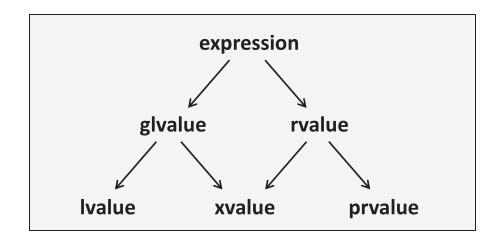
\includegraphics[scale=0.8]{../imgs/05.1.png}
    \caption{从C++11起的值类型体系}
    \label{f5.1}
\end{figure}

\emph{\textbf{lvalue(左值)}}的例子有:
\begin{itemize}
    \item 只含有单个变量、函数或成员的表达式
    \item 只含有字符串字面量的表达式
    \item 内建的一元\texttt{*}运算符(解引用运算符)的结果
    \item 一个返回lvalue(左值)引用(\emph{type\&})的函数的返回值
\end{itemize}
\emph{\textbf{prvalue(纯右值)}}的例子有:
\begin{itemize}
    \item 除字符串字面量和用户自定义字面量之外的字面量组成的表达式
    \item 内建的一元\texttt{\&}运算符(取地址运算符)的运算结果
    \item 内建的数学运算符的结果
    \item 一个返回值的函数的返回值
    \item 一个lambda表达式
\end{itemize}
\emph{\textbf{xvalue(到期值)}}的例子有:
\begin{itemize}
    \item 一个返回rvalue(右值)引用(\emph{type\&\&})的函数的返回值
    (尤其是\texttt{std::move()}的返回值)
    \item 把一个对象转换为rvalue(右值)引用的操作的结果
\end{itemize}
简单来讲:
\begin{itemize}
    \item 所有用作表达式的变量名都是\emph{lvalue(左值)}。
    \item 所有用作表达式的字符串字面量是\emph{lvalue(左值)}。
    \item 所有其他的字面量(\texttt{4.2, true, nullptr})是\emph{prvalue(纯右值)}。
    \item 所有临时对象(尤其是以值返回的对象)是\emph{prvalue(纯右值)}。
    \item \texttt{std::move()}的结果是一个\emph{xvalue(到期值)}
\end{itemize}
例如:
\begin{lstlisting}
    class X {
    };
    X v;
    const X c;

    void f(const X&);   // 接受任何值类型
    void f(X&&);        // 只接受prvalue和xvalue,但是相比上边的版本是更好的匹配

    f(v);               // 给第一个f()传递了一个可修改lvalue
    f(c);               // 给第一个f()传递了不可修改的lvalue
    f(X());             // 给第二个f()传递了一个prvalue
    f(std::move(v));    // 给第二个f()传递了一个xvalue
\end{lstlisting}
值得强调的一点是严格来讲glvalue(广义左值)、prvalue(纯右值)、xvalue(到期值)是描述表达式的术语
而\emph{不是}描述值的术语(这意味着这些术语其实是误称)。例如,一个变量自身并不是左值,
只含有这个变量的表达式才是左值:
\begin{lstlisting}
    int x = 3;  // 这里,x是一个变量,不是一个左值
    int y = x;  // 这里,x是一个左值
\end{lstlisting}
在第一条语句中,\texttt{3}是一个纯右值,用它初始化了变量(不是左值)\texttt{x}。
在第二条语句中,\texttt{x}是一个左值(该表达式的求值结果指向一个包含有数值\texttt{3}的对象)。
左值\texttt{x}被转换为一个纯右值,然后用来初始化\texttt{y}。

\subsection{自从C++17起的值类型体系}
C++17再次明确了值类型体系,现在的值类型体系如\hyperref[f5.2]{图5.2}所示:

\begin{figure}[htb]
    \begin{center}
        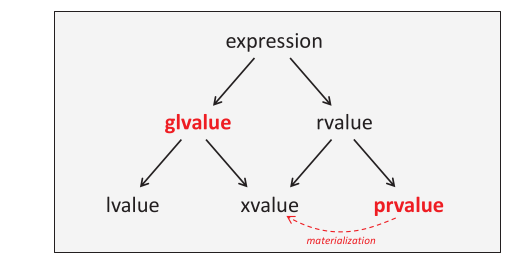
\includegraphics[scale=0.8]{../imgs/05.2.png}
        \caption{自从C++17起的值类型体系}
        \label{f5.2}
    \end{center}
\end{figure}

理解值类型体系的关键是现在广义上来说,我们只有两种类型的表达式:
\begin{itemize}
    \item \textbf{glvaue:} 描述对象或函数\emph{位置}的表达式
    \item \textbf{prvalue:} 用于\emph{初始化}的表达式
\end{itemize}
而\textbf{xvalue}可以认为是一种特殊的位置,它代表一个资源可以被回收利用的对象
(通常是因为该对象的生命周期即将结束)。

C++17引入了一个新的术语:(临时对象的)\emph{实质化(materialization)},
目前prvalue就是一种临时对象。
因此,\emph{临时对象实质化转换(temporary materialization conversion)}
是一种prvalue到xvalue的转换。

在任何情况下prvalue出现在需要glvalue(lvalue或者xvalue)的地方都是有效的,
此时会创建一个临时对象并用该prvalue来初始化(注意prvalue主要就是用来初始化的值)。
然后该prvalue会被临时创建的xvalue类型的临时对象替换。因此上面的例子严格来讲是这样的:
\begin{lstlisting}
    void f(const X& p); // 接受一个任何值类型体系的表达式
                        // 但实际上需要一个glvalue
    f(X());             // 传递了一个prvalue,该prvalue实质化为xvalue
\end{lstlisting}
因为这个例子中的\texttt{f()}的形参是一个引用,所以它需要glvaue类型的实参。
然而,表达式\texttt{X()}是一个prvalue。此时“临时变量实质化”规则会产生作用,
表达式\texttt{X()}会“转换为”一个xvalue类型的临时对象。

注意实质化的过程中并没有创建新的/不同的对象。左值引用\texttt{p}仍然\emph{绑定到}
xvalue和prvalue,尽管后者现在会转换为一个xvalue。

因为prvalue不再是对象而是可以被用来初始化对象的表达式,
所以当使用prvalue来初始化对象时不再需要prvalue是可移动的,
进而省略临时变量拷贝的特性可以完美实现。
我们现在只需要简单的传递初始值,然后它会被自动\emph{实质化}来初始化新对象。
\footnote{感谢Richard Smith和Graham Haynes指出这一点}


\section{未实质化的返回值传递}
所有以值返回临时对象(prvalue)的过程都是在传递未实质化的返回值:
\begin{itemize}
    \item 当我们返回一个非字符串字面量的字面量时:
    \begin{lstlisting}
    int f1() {  // 以值返回int
        return 42;
    }
    \end{lstlisting}
    \item 当我们用\texttt{auto}或类型名作为返回类型并返回一个临时对象时:
    \begin{lstlisting}
    auto f2() { // 以值返回退化的类型
        ...
        return MyType{...};
    }
    \end{lstlisting}
    \item 当使用\texttt{decltype(auto)}作为返回类型并返回临时对象时:
    \begin{lstlisting}
    decltype(auto) f3() {   // 返回语句中以值返回临时对象
        ...
        return MyType{...}
    }
    \end{lstlisting}
\end{itemize}

注意当初始化表达式(此处是返回语句)是一个创建临时对象(prvalue)的表达式时
\texttt{decltype(auto)}将会推导出值类型。因为我们在这些场景中都是以值返回一个prvalue,
所以我们完全不需要任何拷贝/移动。


\section{后记}
用临时变量初始化时强制省略拷贝由Richard Smith在\url{https://wg21.link/p0135r0}中首次提出。
最终被接受的是Richard Smith发表于\url{https://wg21.link/p0135r1}的提案。
    \chapter{lambda表达式扩展}\label{ch6}
C++11引入的lambda和C++14引入的泛型lambda是一个很大的成功。
它允许我们将函数作为参数传递,这让我们能更轻易的指明一种行为。

C++17扩展了lambda表达式的应用场景:
\begin{itemize}
    \item 在常量表达式中使用(也就是在编译期间使用)
    \item 在需要当前对象的拷贝时使用(例如,当在不同的线程中调用lambda时)
\end{itemize}


\section{\texttt{constexpr} lambda}
自从C++17起,lambda表达式会尽可能的隐式声明\texttt{constexpr}。
也就是说,任何只使用有效的编译期上下文
(例如,只有字面量,没有静态变量,没有虚函数,没有\texttt{try/catch},
没有\texttt{new/delete}的上下文)的lambda都可以被用于编译期。

例如,你可以使用一个lambda表达式计算参数的平方,并将计算结果用作\texttt{std::array<>}的大小,
即使这是一个编译期的参数:
\begin{lstlisting}
    auto squared = [](auto val) {   // 自从C++17起隐式constexpr
        return val*val;
    };
    std::array<int, squared(5)> a;  // 自从C++17起OK => std::array<int, 25>
\end{lstlisting}
使用编译期上下文中不允许的特性将会使lambda失去成为\texttt{constexpr}的能力,
不过你仍然可以在运行时上下文中使用lambda:
\begin{lstlisting}
    auto squared2 = [](auto val) {  // 自从C++17起隐式constexpr
        static int calls = 0;       // OK,但会使该lambda不能成为constexpr
        ...
        return val*val;
    };
    std::array<int, squared2(5)> a;     // ERROR:在编译期上下文中使用了静态变量
    std::cout << squared2(5) << '\n';   // OK
\end{lstlisting}
为了确定一个lambda是否能用于编译期,你可以将它声明为\texttt{constexpr}:
\begin{lstlisting}
    auto squared3 = [](auto val) constexpr {  // 自从C++17起OK
        return val*val;
    };
\end{lstlisting}
如果指明返回类型的话,语法看起来像下面这样:
\begin{lstlisting}
    auto squared3i = [](int val) constexpr -> int {  // 自从C++17起OK
        return val*val;
    };
\end{lstlisting}
关于\texttt{constexpr}函数的规则也适用于lambda:如果一个lambda在运行时上下文中使用,
那么相应的函数体也会在运行时才会执行。

然而,如果在声明了\texttt{constexpr}的lambda内使用了编译期上下文中不允许的特性
将会导致编译错误:\footnote{不允许出现在编译期上下文中的特性有:静态变量、虚函数、
\texttt{try/catch}、\texttt{new/delete}等。}
\begin{lstlisting}
    auto squared4 = [](auto val) constexpr {
        static int calls = 0;  // ERROR:在编译期上下文中使用了静态变量
        ...
        return val*val;
    };
\end{lstlisting}
一个隐式或显式的\texttt{constexpr} lambda的函数调用符也是\texttt{constexpr}。
也就是说,如下定义:
\begin{lstlisting}
    auto squared = [](auto val) {   // 从C++17起隐式constexpr
        return val*val;
    };
\end{lstlisting}
将会被转换为如下\emph{闭包类型(closure type)}:
\begin{lstlisting}
    class CompilerSpecificName {
    public:
        ...
        template<typename T>
        constexpr auto operator() (T val) const {
            return val*val;
        }
    };
\end{lstlisting}
注意,这里生成的闭包类型的函数调用运算符自动声明为\texttt{constexpr}。
自从C++17起,如果lambda被显式或隐式地定义为\texttt{constexpr},
那么生成的函数调用运算符将自动是\texttt{constexpr}。

注意如下定义:
\begin{lstlisting}
    auto squared1 = [](auto val) constexpr {  // 编译期lambda调用
        return val*val;
    };
\end{lstlisting}
和如下定义:
\begin{lstlisting}
    constexpr auto squared2 = [](auto val) {  // 编译期初始化squared2
        return val*val;
    };
\end{lstlisting}
是不同的。

第一个例子中如果(只有)lambda是\texttt{constexpr}那么它可以被用于编译期,
但是\texttt{squared1}可能直到运行期才会被初始化,
这意味着如果静态初始化顺序很重要那么可能导致问题
(例如,可能会导致\emph{static initialization order fiasco})。
如果用lambda初始化的闭包对象是\texttt{constexpr},那么该对象将在程序开始时就初始化,
但lambda可能还是只能在运行时使用。因此,可以考虑使用如下定义:
\begin{lstlisting}
    constexpr auto squared = [](auto val) constexpr {
        return val*val;
    };
\end{lstlisting}

\subsection{使用\texttt{constexpr} lambda}
这里有一个使用\texttt{constexpr} lambda的例子。
假设我们有一个字符序列的哈希函数,这个函数迭代字符串的每一个字符反复更新哈希值:
\footnote{djb2算法的源码见\url{http://www.cse.yorku.ca/~oz/hash.html}。}
\begin{lstlisting}
    auto hashed = [](const char* str) {
        std::size_t hash = 5381;        // 初始化哈希值
        while (*str != '\0') {
            hash = hash * 33 ^ *str++;  // 根据下一个字符更新哈希值
        }
        return hash;
    };
\end{lstlisting}
使用这个lambda,我们可以在编译期初始化不同字符串的哈希值,并定义为枚举:
\begin{lstlisting}
    enum Hashed { beer = hashed("beer"),
                  wine = hashed("wine"),
                  water = hashed("water"), ... };   // OK,编译期哈希
\end{lstlisting}
我们也可以在编译期计算\texttt{case}标签:
\begin{lstlisting}
    switch (hashed(argv[1])) {  // 运行时哈希
        case hashed("beer"):    // OK,编译期哈希
            ...
            break;
        case hashed("wine"):
            ...
            break;
        ...
    }
\end{lstlisting}
注意,这里我们将在编译期调用\texttt{case}标签里的\texttt{hashed},
而在运行期间调用\texttt{switch}表达式里的\texttt{hashed}。

如果我们使用编译期lambda初始化一个容器,那么编译器优化时很可能在编译期就计算出容器的初始值
(这里使用了\hyperref[ch9.2.6.3]{\texttt{std::array}的类模板参数推导}):
\begin{lstlisting}
    std::array arr{ hashed("beer"),
                    hashed("wine"),
                    hashed("water") };
\end{lstlisting}
你甚至可以在\texttt{hashed}函数里联合使用另一个\texttt{constexpr} lambda。
设想我们把\texttt{hashed}里根据当前哈希值和下一个字符值更新哈希值的逻辑定义为一个参数:
\begin{lstlisting}
    auto hashed = [](const char* str, auto combine) {
        std::size_t hash = 5381;            // 初始化哈希值
        while (*str != '\0') {
            hash = combine(hash, *str++);   // 用下一个字符更新哈希值
        }
        return hash;
    };
\end{lstlisting}
这个lambda可以像下面这样使用:
\begin{lstlisting}
    constexpr std::size_t hv1{hashed("wine", [](auto h, char c) {return h*33 + c;})};
    constexpr std::size_t hv2{hashed("wine", [](auto h, char c) {return h*33 ^ c;})};
\end{lstlisting}
这里,我们在编译期通过改变更新逻辑初始化了两个不同的\texttt{"wine"}的哈希值。
两个\texttt{hashed}都是在编译期调用。


\section{向lambda传递\texttt{this}的拷贝}
当在非静态成员函数里使用lambda时,你不能隐式获取对该对象成员的使用权。
也就是说,如果你不捕获\texttt{this}的话你将不能在lambda里使用该对象的任何成员
(即使你用\texttt{this->}来访问也不行):
\begin{lstlisting}
    class C {
    private:
        std::string name;
    public:
        ...
        void foo() {
            auto l1 = [] { std::cout << name << '\n'; };        // ERROR
            auto l2 = [] { std::cout << this->name << '\n'; };  // ERROR
            ...
        }
    };
\end{lstlisting}
在C++11和C++14里,你可以通过值或引用捕获\texttt{this}:
\begin{lstlisting}
    class C {
    private:
        std::string name;
    public:
        ...
        void foo() {
            auto l1 = [this] { std::cout << name << '\n'; };    // OK
            auto l2 = [=] { std::cout << name << '\n'; };       // OK
            auto l3 = [&] { std::cout << name << '\n'; };       // OK
            ...
        }
    };
\end{lstlisting}
然而,问题是即使是用拷贝的方式捕获\texttt{this}实质上获得的也是引用
(因为只会拷贝\texttt{this}\emph{指针})。当lambda的生命周期比该对象的生命周期更长的时候,
调用这样的函数就可能导致问题。比如一个极端的例子是在lambda中开启一个新的线程来完成某些任务,
调用新线程时正确的做法是传递整个对象的拷贝来避免并发和生存周期的问题,而不是传递该对象的引用。
另外有时候你可能只是简单的想向lambda传递当前对象的拷贝。

自从C++14起有了一个解决方案,但可读性和实际效果都比较差:
\begin{lstlisting}
    class C {
    private:
        std::string name;
    public:
        ...
        void foo() {
            auto l1 = [thisCopy=*this] { std::cout << thisCopy.name << '\n'; };
            ...
        }
    };
\end{lstlisting}
例如,当使用了\texttt{=}或者\texttt{\&}捕获了其他对象的时候你可能会在不经意间使用\texttt{this}:
\begin{lstlisting}
    auto l1 = [&, thisCopy=*this] {
        thisCopy.name = "new name";
        std::cout << name << '\n'; // OOPS:仍然使用了原来的name
    };
\end{lstlisting}
自从C++17起,你可以通过\texttt{*this}显式地捕获当前对象的拷贝:
\begin{lstlisting}
    class C {
    private:
        std::string name;
    public:
        ...
        void foo() {
            auto l1 = [*this] { std::cout << name << '\n'; };
            ...
        }
    };
\end{lstlisting}
这里,捕获\texttt{*this}意味着该lambda生成的闭包将存储当前对象的一份\emph{拷贝}。

你仍然可以在捕获\texttt{*this}的同时捕获其他对象,只要没有多个\texttt{this}的矛盾:
\begin{lstlisting}
    auto l2 = [&, *this] { ... };       // OK
    auto l3 = [this, *this] { ... };    // ERROR
\end{lstlisting}
这里有一个完整的例子:
\inputcodefile{lang/lambdathis.cpp}
lambda里捕获了\texttt{*this},所以传递进lambda的是一份拷贝。
因此,即使在\texttt{d}被销毁之后使用捕获的对象也没有问题。

如果我们使用\texttt{[this]}、\texttt{[=]}或者\texttt{[\&]}捕获\texttt{this},
那么新线程将会陷入未定义行为,因为当线程中打印\texttt{name}的时候将会使用一个已经销毁的
对象的成员。


\section{以常量引用捕获}
通过使用一个新的库工具,现在也可以\nameref{ch25.2.1}。


\section{后记}
\texttt{constexpr} lambda由Faisal Vali、Ville Voutilainen和Gabriel Dos Reis在
\url{https://wg21.link/n4487}中首次提出。
最终被接受的是Faisal Vali、Jens Maurer、Richard Smith发表
于\url{https://wg21.link/p0170r1}的提案。

在lambda中捕获\texttt{*this}由H. Carter Edwards、Christian Trott、Hal Finkel、
Jim Reus、Robin Maffeo、Ben Sander\\
在\url{https://wg21.link/p0018r0}中首次提出。
最终被接受的是H. Carter Edwards、Daveed Vandevoorde、Christian Trott、Hal Finkel、
Jim Reus、Robin Maffeo、Ben Sander发表于\url{https://wg21.link/p0180r3}的提案。
    \chapter{新属性和属性特性}\label{ch7}
自从C++11起,就可以指明\emph{属性(attributes)}(允许或者禁用某些警告的注解)。
C++17引入了新的属性,还扩展了属性的使用场景,这样可以带来一些便利。


\section{\texttt{[[nodiscard]]}属性}\label{ch7.1}
新属性\texttt{[[nodiscard]]}可以鼓励编译器在某个函数的返回值未被使用时给出警告
(这并不意味着编译器一定要给出警告)。

\texttt{[[nodiscard]]}通常应该用于防止某些因为返回值未被使用导致的不当行为。
这些不当行为可能是(译者注:请配合下边的例子理解这些不当行为):
\begin{itemize}
    \item \textbf{内存泄露},例如返回值中含有动态分配的内存,但并未使用。
    \item \textbf{未知的或出乎意料的行为},例如因为没有使用返回值而导致了一些奇怪的行为。
    \item \textbf{不必要的开销},例如因为返回值没被使用而进行了一些无意义的行为。
\end{itemize}
这里有一些该属性发挥所用的例子:
\begin{itemize}
    \item 申请资源但自身并不释放,而是将资源返回等待其他函数释放的函数应该被标记为
    \texttt{[[nodiscard]]}。一个典型的例子是申请内存的函数,
    例如\texttt{malloc()}函数或者分配器的\texttt{allocate()}成员函数。

    然而,注意有些函数\emph{可能}会返回一个无需再处理的值。例如,程序员可能会用0字节调用C函数
    \texttt{realloc()}来释放内存,这种情况下的返回值无需之后调用\texttt{free()}函数释放。
    因此,如果把\texttt{realloc()}函数标记为\texttt{[[nodiscard]]}将会适得其反。
    \item 有时如果没有使用返回值将导致函数行为和预期不同,一个很好的例子是\texttt{std::async()}
    (C++11引入)。\texttt{std::async()}会在后台异步地执行一个任务并返回一个可以用来等待
    任务执行结束的句柄(也可以通过它获取返回值或者异常)。然而,如果返回值没有被使用的话该调用
    将变成同步的调用,因为在启动任务的语句结束之后未被使用的返回值的析构函数会立即执行,而析构
    函数会阻塞等待任务运行结束。因此,不使用返回值导致的结果与\texttt{std::async()}的目的
    完全矛盾。将\texttt{std::async()}标记为\texttt{[[nodiscard]]}可以让编译器给出警告。
    \item 另一个例子是成员函数\texttt{empty()},它的作用是检查一个对象(容器/字符串)是否
    为空。程序员经常误用该函数来“清空”容器(删除所有元素):
    \begin{lstlisting}
    cont.empty();
    \end{lstlisting}
    这种对\texttt{empty()}的误用并没有使用返回值,所以\texttt{[[nodiscard]]}可以检查出这种误用:
    \begin{lstlisting}
    class MyContainer {
        ...
    public:
        [[nodiscard]] bool empty() const noexcept;
        ...
    };
    \end{lstlisting}
    这里的属性标记可以帮助检查这种逻辑错误。
\end{itemize}
如果因为某些原因你不想使用一个被标记为\texttt{[[nodiscard]]}的函数的返回值,
你可以把返回值转换为\texttt{void}:
\begin{lstlisting}
    (void)coll.empty(); // 禁止[[nodiscard]]警告
\end{lstlisting}
注意如果成员函数被覆盖或者隐藏时基类中标记的属性不会被继承:
\begin{lstlisting}
    struct B {
        [[nodiscard]] int* foo();
    };

    struct D : B {
        int* foo();
    };

    B b;
    b.foo();        // 警告
    (void)b.foo();  // 没有警告

    D d;
    d.foo();        // 没有警告
\end{lstlisting}
因此你需要给派生类里相应的成员函数再次标记\texttt{[[nodiscard]]}
(除非有某些原因导致你不想在派生类里确保返回值必须被使用)。

你可以把属性标记在函数前的所有修饰符之前,也可以标记在函数名之后:
\begin{lstlisting}
    class C {
        ...
        [[nodiscard]] friend bool operator== (const C&, const C&);
        friend bool operator!= [[nodiscard]] (const C&, const C&);
    };
\end{lstlisting}
把属性放在\texttt{friend}和\texttt{bool}之间或者\texttt{bool}和\texttt{operator==}
之间是错误的。

尽管这个特性从C++17起引入,但它还没有在标准库中使用。因为这个提案出现的太晚了,所以最
需要它的\texttt{std::async()}也还没有使用它。不过这里讨论的所有例子,将在下一次C++标准
中实现(见C++20中通过的\url{https://wg21.link/p0600r1}提案)。

为了保证代码的可移植性,你应该使用\texttt{[[nodiscard]]}而不是一些不可移植的方案
(例如gcc和clang的\\
\texttt{[[gnu:warn\_unused\_result]]}或者Visual C++的\texttt{\_Check\_return\_})。

当\hyperref[ch30.2.2]{定义\texttt{new()}运算符}时,
你应该用\texttt{[[nodiscard]]}对该函数进行标记,
例如\hyperref[ch30.4]{定义一个追踪所有\texttt{new}调用的头文件}。


\section{\texttt{[[maybe\_unused]]}属性}
新的属性\texttt{[[maybe\_unused]]}可以避免编译器在某个变量未被使用时发出警告。
新的属性可以应用于类的声明、使用\texttt{typedef}或者\texttt{using}定义的类型、
一个变量、一个非静态数据成员、一个函数、一个枚举类型、一个枚举值等场景。

例如其中一个作用是定义一个可能不会使用的参数:
\begin{lstlisting}
    void foo(int val, [[maybe_unused]] std::string msg)
    {
    #ifdef DEBUG
        log(msg);
    #endif
        ...
    }
\end{lstlisting}
另一个例子是定义一个可能不会使用的成员:
\begin{lstlisting}
    class MyStruct {
        char c;
        int i;
        [[maybe_unused]] char makeLargerSize[100];
        ...
    };
\end{lstlisting}
注意你不能对一条语句应用\texttt{[[maybe\_unused]]}。
因此,你不能直接用\texttt{[[maybe\_unused]]}来抵消\\
\texttt{[[nodiscard]]}的作用:
\footnote{感谢Roland Bock指出这一点}
\begin{lstlisting}
    [[nodiscard]] void* foo();
    int main()
    {
        foo();                              // 警告:返回值没有使用
        [[maybe_unused]] foo();             // 错误:maybe_unused不允许出现在此
        [[maybe_unused]] auto x = foo();    // OK
    }
\end{lstlisting}


\section{\texttt{[[fallthrough]]}属性}
新的属性\texttt{[[fallthrough]]}可以避免编译器在\texttt{switch}语句中某一个标签
缺少\texttt{break}语句时发出警告。例如:
\begin{lstlisting}
    void commentPlace(int place)
    {
        switch (place) {
            case 1:
                std::cout << "very ";
                [[fallthrough]];
            case 2:
                std::cout << "well\n";
                break;
            default:
                std::cout << "OK\n";
                break;
        }
    }
\end{lstlisting}
这个例子中参数为1时将输出:
\begin{blacklisting}
    very well
\end{blacklisting}
\texttt{case 1}和\texttt{case 2}中的语句都会被执行。
注意这个属性必须被用作单独的语句,还要有分号结尾。
另外在\texttt{switch}语句的最后一个分支不能使用它。


\section{通用的属性扩展}
自从C++17起下列有关属性的通用特性变得可用:
\begin{enumerate}
    \item 属性现在可以用来标记命名空间。例如,你可以像下面这样弃用一个命名空间:
    \begin{lstlisting}
    namespace [[deprecated]] DraftAPI {
        ...
    }
    \end{lstlisting}
    这也可以应用于内联的和匿名的命名空间。
    \item 属性现在可以标记枚举子(枚举类型的值)。
    例如你可以像下面这样引入一个新的枚举值作为某个已有枚举值(并且现在已经被废弃)的替代:
    \begin{lstlisting}
    enum class City { Berlin = 0,
                      NewYork = 1,
                      Mumbai = 2,
                      Bombay [[deprecated]] = Mumbai,
                      ... };
    \end{lstlisting}
    这里\texttt{Mumbai}和\texttt{Bombay}代表同一个城市的数字码,但使用\texttt{Bombay}
    已经被标记为废弃的。注意对于枚举值,属性被放置在标识符\emph{之后}。
    \item 用户自定义的属性一般应该定义在自定义的命名空间中。现在可以使用\texttt{using}前缀
    来避免为每一个属性重复输入命名空间。也就是说,如下代码:
    \begin{lstlisting}
    [[MyLib::WebService, MyLib::RestService, MyLib::doc("html")]] void foo();
    \end{lstlisting}
    可以被替换为
    \begin{lstlisting}
    [[using MyLib: WebService, RestService, doc("html")]] void foo();
    \end{lstlisting}
    注意在使用了\texttt{using}前缀时重复命名空间将导致错误:
    \begin{lstlisting}
    [[using MyLib: MyLib::doc("html")]] void foo(); // ERROR
    \end{lstlisting}
\end{enumerate}


\section{后记}
三个新属性由Andrew Tomazos在\url{https://wg21.link/p0068r0}中首次提出。

\texttt{[[nodiscard]]}属性最终被接受的是Andrew Tomazos发表于
\url{https://wg21.link/p0189r1}的提案。
\texttt{[[maybe\_unused]]}属性最终被接受的是Andrew Tomazos发表于
\url{https://wg21.link/p0212r1}的提案。
\texttt{[[fallthrough]]}属性最终被接受的是Andrew Tomazos发表于
\url{https://wg21.link/p0188r1}的提案。

允许为命名空间和枚举值标记属性由Richard Smith在\url{https://wg21.link/n4196}中首次提出。
最终被接受的是Richard Smith发表于\url{https://wg21.link/n4266}的提案。

属性的\texttt{using}前缀由J. Daniel Garcia、Luis M. Sanchez、
Massimo Torquati、Marco Danelutto、Peter Sommerlad
在\url{https://wg21.link/p0028r0}中首次提出。
最终被接受的是J. Daniel Garcia和Daveed Vandevoorde发表于
\url{https://wg21.link/P0028R4}的提案。
    \chapter{其他语言特性}\label{ch8}
在C++17中还有一些微小的核心语言特性的变更,将在这一章中介绍。

\section{嵌套命名空间}\label{ch8.1}
自从2003年第一次提出,到现在C++标准委员会终于同意了以如下方式定义嵌套的命名空间:
\begin{lstlisting}
    namespace A::B::C {
        ...
    }
\end{lstlisting}
等价于:
\begin{lstlisting}
    namespace A {
        namespace B {
            namespace C {
                ...
            }
        }
    }
\end{lstlisting}
注意目前还没有对嵌套内联命名空间的支持。
这是因为\texttt{inline}是作用于最内层还是整个命名空间还有歧义(两种情况都很有用)。

\section{有定义的表达式求值顺序}\label{ch8.2}
许多C++书籍里的代码如果按照直觉来看似乎是正确的,但严格上讲它们有可能导致未定义的行为。
一个简单的例子是在一个字符串中替换多个子串:
\begin{lstlisting}
    std::string s = "I heard it even works if you don't believe";
    s.replace(0, 8, "").replace(s.find("even", 4, "sometimes")
                       .replace(s.find("you don't"), 9, "I");
\end{lstlisting}
通常的假设是前8个字符被空串替换,\texttt{"even"}被\texttt{"sometimes"}替换,
\texttt{"you don't"}被\texttt{"I"}替换。因此结果是:
\begin{blacklisting}
    it sometimes works if I believe
\end{blacklisting}
然而在C++17之前最后的结果实际上并没有任何保证。因为查找子串位置的\texttt{find()}
函数可能在需要它们的返回值之前的任意时刻调用,而不是像直觉中的那样从左向右按顺序执行表达式。
事实上,所有的\texttt{find()}调用可能在执行第一次替换之前就全部执行,因此结果变为:

\begin{blacklisting}
    it even worsometimesf youIlieve
\end{blacklisting}
其他的结果也是有可能的:
\begin{blacklisting}
    it sometimes workIdon’t believe
    it even worsometiIdon’t believe
\end{blacklisting}
作为另一个例子,考虑使用输出运算符打印几个相互依赖的值:
\begin{lstlisting}
    std::cout << f() << g() << h();
\end{lstlisting}
通常的假设是依次调用\texttt{f()}、\texttt{g()}、\texttt{h()}函数。
然而这个假设实际上是错误的。\texttt{f()}、\texttt{g()}、\texttt{h()}有可能以任意顺序调用,
当这三个函数的调用顺序会影响返回值的时候可能就会出现奇怪的结果。

作为一个具体的例子,直到C++17之前,下面代码的行为都是未定义的:
\begin{lstlisting}
    i = 0;
    std::cout << ++i << ' ' << --i << '\n';
\end{lstlisting}
在C++17之前,它\emph{\textbf{可能}}会输出\texttt{1 0},但也可能输出\texttt{0 -1}
或者\texttt{0 0},这和变量\texttt{i}是\texttt{int}还是用户自定义类型无关(不过对于基本类型,
编译器一般会在这种情况下给出警告)。

为了解决这种未定义的问题,C++17标准重新定义了\emph{一些}运算符的的求值顺序,
因此这些运算符现在有了固定的求值顺序:
\begin{itemize}
    \item 对于运算
    \begin{lstlisting}
    e1 `\textbf{[}` e2 `\textbf{]}`
    e1 `\textbf{.}` e2
    e1 `\textbf{.*}` e2
    e1 `\textbf{->*}` e2
    e1 `\textbf{<<}` e2
    e1 `\textbf{>>}` e2
    \end{lstlisting}
    \emph{e1}现在保证一定会在\emph{e2}之前求值,因此求值顺序是从左向右。
    然而,注意同一个函数调用中的不同参数的计算顺序仍然是未定义的。也就是说:
    \begin{lstlisting}
    e1.f(a1, a2, a3);
    \end{lstlisting}
    中的\texttt{e1.f}保证会在\texttt{a1}、\texttt{a2}、\texttt{a3}之前求值。
    但\texttt{a1}、\texttt{a2}、\texttt{a3}的求值顺序仍是未定义的。
    \item 所有的赋值运算
    \begin{lstlisting}
    e2 `\textbf{=}` e1
    e2 `\textbf{+=}` e1
    e2 `\textbf{*=}` e1
    ...
    \end{lstlisting}
    中右侧的\emph{e1}现在保证一定会在左侧的\emph{e2}之前求值。
    \item 最后,类似于如下的\texttt{new}表达式
    \begin{lstlisting}
    `\textbf{new}` Type(e)
    \end{lstlisting}
    中保证内存分配的操作在对\emph{e}求值之前发生。
    新的对象的初始化操作保证在第一次使用该对象之前完成。
\end{itemize}
所有这些保证适用于所有基本类型和自定义类型。

因此,自从C++17起
\begin{lstlisting}
    std::string s = "I heard it even works if you don't believe";
    s.replace(0, 8, "").replace(s.find("even"), 4, "always")
                       .replace(s.find("don't believe"), 13, "use C++17");
\end{lstlisting}
保证将会把\texttt{s}的值修改为:
\begin{blacklisting}
    it always works if you use C++17
\end{blacklisting}
因为现在每个\texttt{find()}之前的替换操作都保证
会在对该\texttt{find()}表达式求值之前完成。

另一个例子,如下语句:
\begin{lstlisting}
    i = 0;
    std::cout << ++i << ' ' << --i << '\n';
\end{lstlisting}
对于任意类型的\texttt{i}都保证输出是\texttt{1 0}。

然而,其他大多数运算符的运算顺序仍然是未知的。例如:
\begin{lstlisting}
    i = i++ + i;    // 仍然是未定义的行为
\end{lstlisting}
这里,最右侧的\texttt{i}可能在\texttt{i}自增之前求值也可能在自增之后求值。

新的表达式求值顺序的另一个应用是定义一个在参数之前\hyperref[ch11.2.1]{插入空格的函数}。

\subsubsection{向后的不兼容性}
新的有定义的求值顺序可能会影响现有程序的输出。例如,考虑如下程序:
\inputcodefile{lang/evalexcept.cpp}
因为这个程序中的\texttt{vector<>}只有4个元素,因此在\texttt{print10elems()}的循环中
使用无效的索引调用\texttt{at()}时将会抛出异常:
\begin{lstlisting}
    std::cout << "value: " << v.at(i) << "\n";
\end{lstlisting}
在C++17之前,输出可能是:
\begin{blacklisting}
    value: 7
    value: 14
    value: 21
    value: 28
    EXCEPTION: ...
\end{blacklisting}
因为\texttt{at()}允许在输出\texttt{"value: "}之前调用,
所以当索引错误时可以跳过开头的\texttt{"value: "}输出。
\footnote{较旧版本的GCC或者Visual C++的行为就是这样的。}

自从C++17以后,输出保证是:
\begin{blacklisting}
    value: 7
    value: 14
    value: 21
    value: 28
    value: EXCEPTION: ...
\end{blacklisting}
因为现在\texttt{"value: "}的输出保证在\texttt{at()}调用之前。

\section{更宽松的用整型初始化枚举值的规则}\label{ch8.3}
对于一个有固定底层类型的枚举类型变量,自从C++17开始可以用一个整型值直接进行列表初始化。
这可以用于带有明确类型的无作用域枚举和所有有作用域的枚举,因为它们都有默认的底层类型:
\begin{lstlisting}
    // 指明底层类型的无作用域枚举类型
    enum MyInt : char { };
    MyInt i1{42};       // 自从C++17起OK(C++17以前ERROR)
    MyInt i2 = 42;      // 仍然ERROR
    MyInt i3(42);       // 仍然ERROR
    MyInt i4 = {42};    // 仍然ERROR

    // 带有默认底层类型的有作用域枚举
    enum class Weekday { mon, tue, wed, thu, fri, sat, sun };
    Weekday s1{0};      // 自从C++17起OK(C++17以前ERROR)
    Weekday s2 = 0;     // 仍然ERROR
    Weekday s3(0);      // 仍然ERROR
    Weekday s4 = {0};   // 仍然ERROR
\end{lstlisting}
如果\texttt{Weekday}有明确的底层类型的话结果完全相同:
\begin{lstlisting}
    // 带有明确底层类型的有作用域枚举
    enum class Weekday : char { mon, tue, wed, thu, fri, sat, sun };
    Weekday s1{0};      // 自从C++17起OK(C++17以前ERROR)
    Weekday s2 = 0;     // 仍然ERROR
    Weekday s3(0);      // 仍然ERROR
    Weekday s4 = {0};   // 仍然ERROR
\end{lstlisting}
对于\emph{没有}明确底层类型的无作用域枚举类型(没有\texttt{class}的\texttt{enum}),
你仍然不能使用列表初始化:
\begin{lstlisting}
    enum Flag { bit1=1, bit2=2, bit3=4 };
    Flag f1{0};     // 仍然ERROR
\end{lstlisting}
注意列表初始化不允许窄化,所以你不能传递一个浮点数:
\begin{lstlisting}
    enum MyInt : char { };
    MyInt i5{42.2}; // 仍然ERROR
\end{lstlisting}
一个定义新的整数类型的技巧是简单的定义一个以某个已有整数类型作为底层类型的枚举类型,
就像上面例子中的\texttt{MyInt}一样。
这个特性的动机之一就是为了支持这个技巧,如果没有这个特性,在不进行转换的情况下将无法初始化新的对象。

事实上自从C++17起标准库提供的\nameref{ch18}就直接使用了这个特性。

\section{修正\texttt{auto}类型的列表初始化}\label{ch8.4}
自从在C++11中引入了花括号\emph{统一}初始化之后,
每当使用\texttt{auto}代替明确类型进行列表初始化时就会出现一些和直觉不一致的结果:
\begin{lstlisting}
    int x{42};       // 初始化一个int
    int y{1, 2, 3};  // ERROR
    auto a{42};      // 初始化一个std::initializer_list<int>
    auto b{1, 2, 3}; // OK:初始化一个std::initializer_list<int>
\end{lstlisting}
这些\emph{直接}使用列表初始化(没有使用=)时的不一致行为现在已经被修复了。
因此如下代码的行为变成了:
\begin{lstlisting}
    int x{42};       // 初始化一个int
    int y{1, 2, 3};  // ERROR
    auto a{42};      // 现在初始化一个int
    auto b{1, 2, 3}; // 现在ERROR
\end{lstlisting}
注意这是一个\textbf{破坏性的更改(breaking change)},因为它可能导致很多代码的行为在
无声无息中发生改变。因此,支持了这个变更的编译器现在即使在C++11模式下也会启用这个变更。
对于主流编译器,接受这个变更的版本分别是Visual Studio 2015,g++5,clang3.8。

注意当使用\texttt{auto}进行\emph{拷贝列表初始化}(使用了=)时仍然是初始化一个
\texttt{std::initializer\_list<>}:
\begin{lstlisting}
    auto c = {42};      // 仍然初始化一个std::initializer_list<int>
    auto d = {1, 2, 3}; // 仍然OK:初始化一个std::initializer_list<int>
\end{lstlisting}
因此,现在直接初始化(没有=)和拷贝初始化(有=)之间又有了显著的不同:
\begin{lstlisting}
    auto a{42};     // 现在初始化一个int
    auto c = {42};  // 仍然初始化一个std::initializer_list<int>
\end{lstlisting}
这也是更推荐使用直接列表初始化(没有=的花括号初始化)的原因之一。

\section{十六进制浮点数字面量}\label{ch8.5}
C++17允许指定十六进制浮点数字面量(有些编译器甚至在C++17之前就已经支持)。
当需要一个精确的浮点数表示时这个特性非常有用(如果直接用十进制的浮点数字面量不保证
存储的实际精确值是多少)。

例如:
\inputcodefile{lang/hexfloat.cpp}
程序通过使用已有的和新增的十六进制浮点记号定义了不同的浮点数值。
新的记号是一个以2为基数的科学记数法记号:
\begin{itemize}
    \item 有效数字/尾数用十六进制书写
    \item 指数部分用十进制书写,表示乘以2的n次幂
\end{itemize}
例如\texttt{0xAp2}的值为40($10\times2^2$)。这个值也可以被写作\texttt{0x1.4p+5},
也就是$1.25\times32$(0.4是十六进制的分数,等于十进制的0.25,$2^5=32$)。

程序的输出如下:
\begin{blacklisting}
    dec:     16  hex: 0x1p+4
    dec:     10  hex: 0x1.4p+3
    dec:     40  hex: 0x1.4p+5
    dec:      5  hex: 0x1.4p+2
    dec:      5  hex: 0x1.4p+2
    dec: 100000  hex: 0x1.86ap+16
    dec: 100000  hex: 0x1.86ap+16
    dec: 49.625  hex: 0x1.8dp+5
\end{blacklisting}
就像上例展示的一样,十六进制浮点数的记号很早就存在了,
因为输出流使用的\texttt{std::hexfloat}操作符自从C++11起就已经存在了。

\section{UTF-8字符字面量}\label{ch8.6}
自从C++11起,C++就已经支持以\texttt{u8}为前缀的UTF-8字符串字面量。
然而,这个前缀不能用于字符字面量。C++17修复了这个问题,所以现在可以这么写:
\begin{lstlisting}
    auto c = u8'6'; // UTF-8编码的字符6
\end{lstlisting}
在C++17中,\texttt{u8'6'}的类型是\texttt{char},在C++20中可能会变为\texttt{char8\_t},
因此这里使用\texttt{auto}会更好一些。

通过使用该前缀现在可以保证字符值是UTF-8编码。你可以使用所有的7位的US-ASCII字符,
这些字符的UTF-8表示和US-ASCII表示完全相同。
也就是说,\texttt{u8'6'}也是有效的以7位US-ASCII表示的字符'6'
(也是有效的ISO Latin-1、ISO-8859-15、基本Windows字符集中的字符)。
\footnote{ISO Latin-1的正式命名为ISO-8859-1,而为了包含欧元符号€引入的字符集
ISO-8859-15也被命名为ISO Latin-9。}
通常情况下你的源码字符被解释为US-ASCII或者UTF-8的结果是一样的,所以这个前缀并不是必须的。
\texttt{c}的值永远是\texttt{54}(十六进制\texttt{36})。

这里给出一些背景知识来说明这个前缀的必要性:对于源码中的字符和字符串字面量,
C++标准化了你可以使用的字符而不是这些字符的值。这些值取决于\emph{源码字符集}。
当编译器为源码生成可执行程序时它使用\emph{运行字符集}。源码字符集几乎总是7位的
US-ASCII编码,而运行字符集通常是相同的。这意味着在任何C++程序中,所有相同的字符和字符串字面量
(不管有没有\texttt{u8}前缀)总是有相同的值。

然而,在一些特别罕见的场景中并不是这样的。例如,在使用EBCDIC字符集的旧的IBM机器上,字符'6'
的值将是246(十六进制为F6)。在一个使用EBCDIC字符集的程序中上面的字符\texttt{c}的值将是
246而不是54,如果在UTF-8编码的平台上运行这个程序可能会打印出字符ö,这个字符在ISO/IEC 8859-x
编码中的值为246.在这种情况下,这个前缀就是必须的。

注意\texttt{u8}只能用于单个字符,并且该字符的UTF-8编码必须只占一个字节。一个如下的初始化:
\begin{lstlisting}
    char c = u8'ö';
\end{lstlisting}
是不允许的,因为德语的曲音字符ö的UTF-8编码是两个字节的序列,分别是195和182(十六进制为C3 B6)。

因此,字符和字符串字面量现在接受如下前缀:
\begin{itemize}
    \item u8用于单字节US-ASCII和UTF-8编码
    \item u用于两字节的UTF-16编码
    \item U用于四字节的UTF-32编码
    \item L用于没有明确编码的宽字符,可能是两个或者四个字节
\end{itemize}

\section{异常声明作为类型的一部分}\label{ch8.7}
自从C++17之后,异常处理声明变成了函数类型的一部分。也就是说,如下的两个函数的类型是不同的:
\begin{lstlisting}
    void fMightThrow();
    void fNoexcept() noexcept;  // 不同类型
\end{lstlisting}
在C++17之前这两个函数的类型是相同的。这样的一个问题就是如果把一个可能抛出异常的函数赋给
一个保证不抛出异常的函数指针,那么调用时有可能会抛出异常:
\footnote{这样看起来好像是一个错误,但至少之前g++的确允许这种行为。}
\begin{lstlisting}
    void (*fp)() noexcept;  // 指向不抛异常的函数的指针
    fp = fNoexcept;         // OK
    fp = fMightThrow;       // 自从C++17起ERROR
\end{lstlisting}
把一个不会抛出异常的函数赋给一个可能抛出异常的函数指针仍然是有效的:
\begin{lstlisting}
    void (*fp2)();      // 指向可能抛出异常的函数的指针
    fp2 = fNoexcept;    // OK
    fp2 = fMightThrow;  // OK
\end{lstlisting}
因此,如果程序中只使用了没有\texttt{noexcept}声明的函数指针,那么将不会受该特性影响。
但请注意现在不能再违反函数指针中的\texttt{noexcept}声明(这可能会善意的破坏现有的程序)。

重载一个签名完全相同只有异常声明不同的函数是不允许的(就像不允许重载只有返回值不同的函数一样):
\begin{lstlisting}
    void f3();
    void f3() noexcept;     // ERROR
\end{lstlisting}
注意其他的规则不受影响。例如,你仍然不能忽略基类中的\texttt{noexcept}声明:
\begin{lstlisting}
    class Base {
    public:
        virtual void foo() noexcept;
        ...
    };

    class Derived : public Base {
    public:
        void foo() override;    // ERROR:不能重载
        ...
    };
\end{lstlisting}
这里,派生类中的成员函数\texttt{foo()}和基类中的\texttt{foo()}类型不同所以不能重载。
这段代码不能通过编译,即使没有\texttt{override}修饰符代码也不能编译,因为我们不能用
更宽松的异常声明重载。

\subsubsection{使用传统的异常声明}
当使用传统的\texttt{noexcept}声明时,函数的是否抛出异常取决于条件为true还是false:
\begin{lstlisting}
    void f1();
    void f2() noexcept;
    void f3() noexcept(sizeof(int)<4);  // 和f1()或f2()的类型相同
    void f4() noexcept(sizeof(int)>=4); // 和f3()的类型不同
\end{lstlisting}
这里\texttt{f3()}的类型取决于条件的值:
\begin{itemize}
    \item 如果\texttt{sizeof(int)}返回4或者更大,签名等价于
    \begin{lstlisting}
    void f3() noexcept(false); // 和f1()类型相同
    \end{lstlisting}
    \item 如果\texttt{sizeof(int)}返回的值小于4,签名等价于
    \begin{lstlisting}
    void f3() noexcept(true);  // 和f2()类型相同
    \end{lstlisting}
\end{itemize}
因为\texttt{f4()}的异常条件和\texttt{f3()}的恰好相反,所以\texttt{f3()}和\texttt{f4()}
的类型总是不同(也就是说,它们一定是一个可能抛异常,另一个不可能抛异常)。

旧式的不抛异常的声明仍然有效但自从C++11起就被废弃:
\begin{lstlisting}
    void f5() throw();  // 和void f5() noexcept等价但已经被废弃
\end{lstlisting}
带参数的动态异常声明不再被支持(自从C++11起被废弃):
\begin{lstlisting}
    void f6() throw(std::bad_alloc); // ERROR:自从C++17起无效
\end{lstlisting}

\subsubsection{对泛型库的影响}
将\texttt{noexcept}做为类型的一部分意味着会对泛型库产生一些影响。例如,下面的代码
直到C++14是有效的,但从C++17起不能再通过编译:
\inputcodefile{lang/noexceptcalls.cpp}
问题在于自从C++17起\texttt{f1()}和\texttt{f2()}的类型不再相同,
因此在实例化模板函数\texttt{call()时}编译器无法推导出类型\texttt{T},

自从C++17起,你需要指定两个不同的模板参数来通过编译:
\begin{lstlisting}
    template<typename T1, typename T2>
    void call(T1 op1, T2 op2)
    {
        op1();
        op2();
    }
\end{lstlisting}
现在如果你想重载所有可能的函数类型,那么你需要重载的数量将是原来的两倍。
例如,对于标准库类型特征\texttt{std::is\_function<>}的定义,
主模板的定义如下,该模板用于匹配\texttt{T}不是函数的情况:
\begin{lstlisting}
    // 主模板(匹配泛型类型T不是函数的情况):
    template<typename T> struct is_function : std::false_type { };
\end{lstlisting}
该模板从\hyperref[ch33.2]{\texttt{std::false\_type}}派生,
因此\texttt{is\_function<T>::value}对任何类型\texttt{T}都会返回\texttt{false}。

对于任何\emph{是}函数的类型,存在从\hyperref[ch33.2]{\texttt{std::true\_type}}
派生的部分特化版,因此成员\texttt{value}总是返回\texttt{true}:
\begin{lstlisting}
    // 对所有函数类型的部分特化版
    template<typename Ret, typename... Params>
    struct is_function<Ret (Params...)> : std::true_type { };

    template<typename Ret, typename... Params>
    struct is_function<Ret (Params...) const> : std::true_type { };

    template<typename Ret, typename... Params>
    struct is_function<Ret (Params...) &> : std::true_type { };

    template<typename Ret, typename... Params>
    struct is_function<Ret (Params...) const &> : std::true_type { };
    ...
\end{lstlisting}
在C++17之前该特征总共有24个部分特化版本:因为函数类型可以用\texttt{const}
和\texttt{volatile}修饰符修饰,另外还可能有左值引用(\&)或右值引用(\&\&)修饰符,
还需要重载可变参数列表的版本。

现在在C++17中部分特化版本的数量变为了两倍,因为还需要为所有版本添加一个带\texttt{noexcept}
修饰符的版本:
\begin{lstlisting}
    ...
    // 对所有带有noexcept声明的函数类型的部分特化版本
    template<typename Ret, typename... Params>
    struct is_function<Ret (Params...) noexcept> : std::true_type { };

    template<typename Ret, typename... Params>
    struct is_function<Ret (Params...) const noexcept> : std::true_type { };

    template<typename Ret, typename... Params>
    struct is_function<Ret (Params...) & noexcept> : std::true_type { };

    template<typename Ret, typename... Params>
    struct is_function<Ret (Params...) const & noexcept> : std::true_type { };
    ...
\end{lstlisting}
那些没有实现\texttt{noexcept}重载的库可能在需要使用带有
\texttt{noexcept}的函数的场景中不能通过编译了。

\section{单参数\texttt{static\_assert}}\label{ch8.8}
自从C++17起,以前\texttt{static\_assert()}要求的用作错误信息的参数变为可选的了。
也就是说现在断言失败时输出的诊断信息完全依赖平台的实现。例如:
\begin{lstlisting}
    #include <type_traits>

    template<typename t>
    class C {
        // 自从C++11起OK
        static_assert(std::is_default_constructible<T>::value,
                      "class C: elements must be default-constructible");

        // 自从C++17起OK
        static_assert(std::is_default_constructible_v<T>);
        ...
    };
\end{lstlisting}
不带错误信息参数的新版本静态断言的示例也使用了\nameref{ch21.1}。

\section{预处理条件\texttt{\_\_has\_include}}\label{ch8.9}
C++17扩展了预处理,增加了一个检查某个头文件是否可以被包含的宏。例如:
\begin{lstlisting}
    #if __has_include(<filesystem>)
    #  include <filesystem>
    #  define HAS_FILESYSTEM 1
    #elif __has_include(<experimental/filesystem>)
    #  include <experimental/filesystem>
    #  define HAS_FILESYSTEM 1
    #  define FILESYSTEM_IS_EXPERIMENTAL 1
    #elif __has_include("filesystem.hpp")
    #  include "filesystem.hpp"
    #  define HAS_FILESYSTEM 1
    #  define FILESYSTEM_IS_EXPERIMENTAL 1
    #else
    #  define HAS_FILESYSTEM 0
    #endif
\end{lstlisting}
当相应的\texttt{\#include}指令有效时\texttt{\_\_has\_include(...)}会被求值为1。
其他的因素都不会影响结果(例如,相应的头文件是否已被包含过并不影响结果)。

另外,虽然求值为真可以说明相应的头文件确实存在但不能保证它的内容符合预期。
它的内容可能是空的或者无效的。

\texttt{\_\_has\_include}是一个纯粹的预处理指令。
所以不能将它用作源码里的条件表达式:
\begin{lstlisting}
    if (__has_include(<filesystem>)) {  // ERROR
    }
\end{lstlisting}

\section{后记}
\hyperref[ch8.1]{嵌套命名空间定义}由Jon Jagger于2003年在
\url{https://wg21.link/n1524}中首次提出。
Robert Kawulak于2014年在\url{https://wg21.link/n4026}中提出了新的提案。
最终被接受的是Robert Kawulak和Andrew Tomazos发表于\url{https://wg21.link/n4230}的提案。

\nameref{ch8.2}由Gabriel Dos Reis、Herb Sutter、Jonathan Caves在
\url{https://wg21.link/n4228}中首次提出。最终被接受的是Gabriel Dos Reis、
Herb Sutter和Jonathan Caves发表于\url{https://wg21.link/p0145r3}的提案。

\nameref{ch8.3}由Gabriel Dos Reis在\url{https://wg21.link/p0138r0}中首次提出。
最终被接受的是Gabriel Dos Reis发表于\url{https://wg21.link/p0138r2}的提案。

\nameref{ch8.4}由Ville Voutilainen在\url{https://wg21.link/n3681}以及
\url{https://wg21.link/3912}中首次提出。\texttt{auto}列表初始化最终的修正由
James Dennett在\url{https://wg21.link/n3681}提出。

\nameref{ch8.5}由Thomas Köppe在\url{https://wg21.link/p0245r0}中首次提出。
最终被接受的是Thomas Köppe发表于\url{https://wg21.link/p0245r1}的提案。

\nameref{ch8.6}是由Richard Smith在\url{https://wg21.link/n4197}中首次提出。
最终被接受的是Richard Smith发表于\url{https://wg21.link/n4267}的提案。

\nameref{ch8.7}由Jens Maurer在\url{https://wg21.link/n4320}中首次提出。
最终被接受的是Jens Maurer发表于\url{https://wg21.link/p0012r1}的提案。

\nameref{ch8.8}被接受的是Walter E. Brown发表于\url{https://wg21.link/n3928}的提案。

\hyperref[ch8.9]{预处理语句\texttt{\_\_has\_include()}}由Clark Nelson和Richard Smith在
\url{https://wg21.link/p0061r0}的某一部分中首次提出。
最终被接受的是Clark Nelson和Richard Smith发表于\url{https://wg21.link/p0061r1}的提案。



    \part{模板特性}\label{part2}
    这一部分介绍了C++17为泛型编程(即模板)提供的新的语言特性。

    我们首先从类模板参数推导开始,这一特性只影响模板的使用。之后的章节会介绍为编写泛型代码
    (函数模板,类模板,泛型库等)的程序员提供的新特性。

    \chapter{类模板参数推导}\label{ch9}
在C++17之前,你必须明确指出类模板的所有参数。
例如,你不可以省略下面的\texttt{double}:
\begin{lstlisting}
    std::complex<double> c{5.1, 3.3};
\end{lstlisting}
也不可以省略下面代码中的第二个\texttt{std::mutex}:
\begin{lstlisting}
    std::mutex mx;
    std::lock_guard<std::mutex> lg(mx);
\end{lstlisting}
自从C++17起必须指明类模板参数的限制被放宽了。
通过使用\emph{类模板参数推导(class template argument deduction)}(CTAD),
只要编译器能根据初始值\emph{推导出}所有模板参数,那么就可以不指明参数。

例如:
\begin{itemize}
    \item 你现在可以这么声明:
    \begin{lstlisting}
    std::complex c{5.1, 3.3};   // OK:推导出std::complex<double>
    \end{lstlisting}
    \item 你现在可以这么写:
    \begin{lstlisting}
    std::mutex mx;
    std::lock_guard lg{mx};     // OK:推导出std::lock_guard<std::mutex>
    \end{lstlisting}
    \item 你现在甚至可以让容器来推导元素类型:
    \begin{lstlisting}
    std::vector v1 {1, 2, 3};            // OK:推导出std::vector<int>
    std::vector v2 {"hello", "world"};   // OK:推导出std::vector<const char*>
    \end{lstlisting}
\end{itemize}

\section{使用类模板参数推导}
只要能根据初始值推导出所有模板参数就可以使用类模板参数推导。
推导过程支持所有方式的初始化(只要保证初始化是有效的):
\begin{lstlisting}
    std::complex c1{1.1, 2.2};  // 推导出std::complex<double>
    std::complex c2(2.2, 3.3);  // 推导出std::complex<double>
    std::complex c3 = 3.3;      // 推导出std::complex<double>
    std::complex c4 = {4.4};    // 推导出std::complex<double>
\end{lstlisting}
因为\texttt{std::complex}只需要一个参数就可以初始化并推导出模板参数\texttt{T}:
\begin{lstlisting}
    namespace std {
        template<typename T>
        class complex {
            constexpr complex(const T&re = T(), const T& im = T());
            ...
        }
    };
\end{lstlisting}
所以\texttt{c3}和\texttt{c4}可以正确初始化。
对于如下声明:
\begin{lstlisting}
    std::complex c1{1.1, 2.2};
\end{lstlisting}
编译器会查找到构造函数:
\begin{lstlisting}
    constexpr complex(const T& re = T(), const T& im = T());
\end{lstlisting}
并调用。因为两个参数都是\texttt{double}类型,因此编译器会推导出\texttt{T}就是
\texttt{double}并生成如下代码:
\begin{lstlisting}
    complex<double>::complex(const double& re = double(), const double& im = double());
\end{lstlisting}
注意推导的过程中模板参数必须没有歧义。也就是说,如下初始化代码不能通过编译:
\begin{lstlisting}
    std::complex c5{5, 3.3};    // ERROR:尝试将T推导为int和double
\end{lstlisting}
像通常的模板一样,推导模板参数时不会使用隐式类型转换。

也可以对可变参数模板使用类模板参数推导。例如,对于一个如下定义的\texttt{std::tuple}:
\begin{lstlisting}
    namespace std {
        template<typename... Types>
        class tuple {
        public:
            constexpr tuple(const Types&...);
            ...
        };
    };
\end{lstlisting}
如下声明:
\begin{lstlisting}
    std::tuple t{42, 'x', nullptr};
\end{lstlisting}
将推导出类型\texttt{std::tuple<int, char, std::nullptr\_t>}。

你也可以推导非类型模板参数。
例如,我们可以根据传入的参数同时推导数组的元素类型和元素数量:
\begin{lstlisting}
    template<typename T, int SZ>
    class MyClass {
    public:
        MyClass (T(&)[SZ]) {
            ...
        }
    };

    MyClass mc("hello");    // 推导出T为const char,SZ为6
\end{lstlisting}
这里我们推导出\texttt{SZ}为\texttt{6},因为传入的字符串字面量有6个字符。
\footnote{注意构造函数里以引用作为参数是必须的。
否则根据语言规则传入的字符数组将会退化为指针,然后将无法推导出\texttt{SZ}。}

你甚至可以推导\hyperref[ch14.1]{用作基类的lambda}来实现重载
或者推导\hyperref[ch13.1]{\texttt{auto}模板参数}。

\subsection{默认以拷贝方式推导}\label{ch9.1.1}
类模板参数推导过程中会首先尝试以拷贝的方式初始化。
例如,首先初始化一个只有一个元素的\texttt{std::vector}:
\begin{lstlisting}
    std::vector v1{42};         // 一个元素的vector<int>
\end{lstlisting}
然后使用这个vector初始化另一个vector,推导时会解释为创建一个拷贝:
\begin{lstlisting}
    std::vector v2{v1};         // v2也是一个std::vector<int>
\end{lstlisting}
而不是创建一个只有一个元素的\texttt{vector<vector<int>>}。

这个规则适用于所有形式的初始化:
\begin{lstlisting}
    std::vector v2{v1};         // v2也是vector<int>
    std::vector v3(v1);         // v3也是vector<int>
    std::vector v4 = {v1};      // v4也是vector<int>
    auto v5 = std::vector{v1};  // v5也是vector<int>
\end{lstlisting}
注意这是花括号初始化总是把列表中的参数作为元素这一规则的一个例外。
如果你传递一个只有一个vector的初值列来初始化另一个vector,
你将得到一个传入的vector的拷贝。然而,如果用多于一个元素的初值列来初始化的话
就会把传入的参数作为元素并推导出其类型作为模板参数(因为这种情况下无法解释为创建拷贝):
\begin{lstlisting}
    std::vector vv{v1, v2};     // vv是一个vector<vector<int>>
\end{lstlisting}
这引出了一个问题就是对可变参数模板使用类模板参数推导时会发生什么:
\begin{lstlisting}
    template<typename... Args>
    auto make_vector(const Args&... elems) {
        return std::vector{elem...};
    }

    std::vector<int> v{1, 2, 3};
    auto x1 = make_vector(v, v); // vector<vector<int>>
    auto x2 = make_vector(v);    // vector<int>还是vector<vector<int>>?
\end{lstlisting}
目前不同的编译器会有不同的行为,这个问题还在讨论之中。

\subsection{推导lambda的类型}
通过使用类模板参数推导,我们可以用lambda的类型(确切的说是lambda生成的\emph{闭包类型})
作为模板参数来实例化类模板。例如我们可以提供一个泛型类,对一个任意回调函数进行包装并统计调用次数:
\inputcodefile{tmpl/classarglambda.hpp}
这里构造函数获取一个回调函数并进行包装,这样在初始化时会把参数的类型推导为\texttt{CB}。
例如,我们可以使用一个lambda作为参数来初始化一个对象:
\begin{lstlisting}
    CountCalls sc{[](auto x, auto y) { return x > y; }};
\end{lstlisting}
这意味着排序准则\texttt{sc}的类型将被推导为\texttt{CountCalls<}\emph{TypeOfTheLambda}
\texttt{>}。这样,我们可以统计出排序准则被调用的次数:
\begin{lstlisting}
    std::sort(v.begin(), v.end(),   // 排序区间
              std::ref(sc));        // 排序准则
    std::cout << "sorted with " << sc.count() << " calls\n";
\end{lstlisting}
这里包装过后的lambda被用作排序准则。注意这里必须要传递引用,否则\texttt{std::sort()}将会
获取\texttt{sc}的拷贝作为参数,计数时只会修改该拷贝内的计数器。

然而,我们可以直接把包装后的lambda传递给\texttt{std::for\_each()},
因为该算法(非并行版本)最后会返回传入的回调函数,以便于获取回调函数最终的状态:
\begin{lstlisting}
    auto fo = std::for_each(v.begin(), v.end(), CountCalls{[](auto i) {
                                                    std::cout << "elem: " << i << '\n';
                                                }});
    std::cout << "output with " << fo.count() << " calls\n";
\end{lstlisting}
输出将会如下(排序准则调用次数可能会不同,因为\texttt{sort()}的实现可能会不同):
\begin{blacklisting}
    sorted with 39 calls
    elem: 19
    elem: 17
    elem: 13
    elem: 11
    elem: 9
    elem: 7
    elem: 5
    elem: 3
    elem: 2
    output with 9 calls
\end{blacklisting}
如果计数器是原子的,你也可以使用\hyperref[ch22]{并行算法}:
\begin{lstlisting}
    std::sort(std::execution::par, v.begin(), v.end(), std::ref(sc));
\end{lstlisting}

\subsection{没有类模板部分参数推导}
注意,不像函数模板,类模板不能只指明一部分模板参数,然后指望编译器去推导剩余的部分参数。
甚至使用\texttt{<>}指明空模板参数列表也是不允许的。例如:
\begin{lstlisting}
    template<typename T1, typename T2, typename T3 = T2>
    class C
    {
    public:
        C (T1 x = {}, T2 y = {}, T3 z = {}) {
            ...
        }
        ...
    };

    // 推导所有参数
    C c1(22, 44.3, "hi");   // OK:T1是int,T2是double,T3是const char*
    C c2(22, 44.3);         // OK:T1是int,T2和3是double
    C c3("hi", "guy");      // OK:T1、T2、T3都是const char*

    // 推导部分参数
    C<string> c4("hi", "my");   // ERROR:只有T1显式指明
    C<> c5(22, 44.3);           // ERROR:T1和T2都没有指明
    C<> c6(22, 44.3, 42);       // ERROR:T1和T2都没有指明

    // 指明所有参数
    C<string, string, int> c7;              // OK:T1、T2是string,T3是int
    C<int, string> c8(52, "my");            // OK:T1是int,T2、T3是string
    C<string, string> c9("a", "b", "c");    // OK:T1、T2、T3都是string
\end{lstlisting}
注意第三个模板参数有默认值,因此只要指明了第二个参数就不需要再指明第三个参数。

如果你想知道为什么不支持部分参数推导,这里有一个导致这个决定的例子:
\begin{lstlisting}
    std::tuple<int> t(42, 43);  // 仍然ERROR
\end{lstlisting}
\texttt{std::tuple}是一个可变参数模板,因此你可以指明任意数量的模板参数。
在这个例子中,并不能判断出只指明一个参数是一个错误还是故意的。

不幸的是,不支持部分参数推导意味着一个常见的编码需求并没有得到解决。
我们仍然不能简单的使用一个lambda作为关联容器的排序准则或者无序容器的hash函数:
\begin{lstlisting}
    std::set<Cust> coll([] (const Cust& x, const Cust& y) { // 仍然ERROR
                            return x.getName() > y.getName();
                        });
\end{lstlisting}
我们仍然必须指明lambda的类型。例如:
\begin{lstlisting}
    auto sortcrit = [] (const Cust& x, const Cust& y) {
                        return x.getName() > y.getName();
                    };
    std::set<Cust, decltype(sortcrit)> coll(sortcrit);      // OK
\end{lstlisting}
仅仅指明类型是不行的,因为容器初始化时会尝试用给出的lambda类型创建一个lambda。
但这在C++17中是不允许的,因为默认构造函数只有编译器才能调用。
在C++20中如果lambda不需要捕获任何东西的话这将成为可能。

\subsection{使用类模板参数推导代替快捷函数}\label{ch9.1.4}
原则上讲,通过使用类模板参数推导,我们可以摆脱已有的几个快捷函数模板,
这些快捷函数的作用其实就是根据传入的参数实例化相应的类模板。

一个明显的例子是\texttt{std::make\_pair()},它可以帮助我们避免指明传入参数的类型。
例如,在如下声明之后:
\begin{lstlisting}
    std::vector<int> v;
\end{lstlisting}
我们可以这样:
\begin{lstlisting}
    auto p = std::make_pair(v.begin(), v.end());
\end{lstlisting}
而不需要写:
\begin{lstlisting}
    std::pair<typename std::vector<int>::iterator, typename std::vector<int>::iterator>
        p(v.begin(), v.end());
\end{lstlisting}
现在这种场景已经不再需要\texttt{std::make\_pair()}了,我们可以简单的写为:
\begin{lstlisting}
    std::pair p(v.begin(), v.end());
\end{lstlisting}
或者:
\begin{lstlisting}
    std::pair p{v.begin(), v.end());
\end{lstlisting}

然而,从另一个角度来看\texttt{std::make\_pair()}也是一个很好的例子,
它演示了有时便捷函数的作用不仅仅是推导模板参数。
事实上\texttt{std::make\_pair()}会使传入的参数退化
(在C++03中以值传递,自从C++11起使用特征)。
这样会导致字符串字面量的类型(字符数组)被推导为\texttt{const char*}:
\begin{lstlisting}
    auto q = std::make_pair("hi", "world"); // 推导为指针的pair
\end{lstlisting}
这个例子中,\texttt{q}的类型为\texttt{std::pair<const char*, const char*>}。

使用类模板参数推导可能会让事情变得更加复杂。
考虑如下这个类似于\texttt{std::pair}的简单的类的声明:
\begin{lstlisting}
    template<typename T1, typename T2>
    struct Pair1 {
        T1 first;
        T2 second;
        Pair1(const T1& x, const T2& y) : first{x}, second{y} {
        }
    };
\end{lstlisting}
这里元素以引用传入,根据语言规则,当以引用传递参数时模板参数的类型不会退化。
因此,当调用:
\begin{lstlisting}
    Pair1 p1{"hi", "world"}; // 推导为不同大小的数组的pair,但是……
\end{lstlisting}
\texttt{T1}被推导为\texttt{char[3]},\texttt{T2}被推导为\texttt{char[6]}。
原则上讲这样的推导是有效的。然而,我们使用了\texttt{T1}和\texttt{T2}来声明成员
\texttt{first}和\texttt{second},因此它们被声明为:
\begin{lstlisting}
    char first[3];
    char second[6];
\end{lstlisting}
然而使用一个左值数组来初始化另一个数组是不允许的。它类似于尝试编译如下代码:
\begin{lstlisting}
    const char x[3] = "hi";
    const char y[6] = "world";
    char first[3] {x};  // ERROR
    char second[6] {y}; // ERROR
\end{lstlisting}
注意如果我们声明参数时以值传参就不会再有这个问题:
\begin{lstlisting}
    tempalte<typename T1, typename T2>
    struct Pair2 {
        T1 first;
        T2 second;
        Pair2(T1 x, T2 y) : first{x}, second{y} {
        }
    };
\end{lstlisting}
如果我们像下面这样创建新对象:
\begin{lstlisting}
    Pair2 p2{"hi", "world"};    // 推导为指针的pair
\end{lstlisting}
\texttt{T1}和\texttt{T2}都会被推导为\texttt{const char*}。

然而,因为\texttt{std::pair<>}的构造函数以引用传参,
所以下面的初始化正常情况下应该不能通过编译:
\begin{lstlisting}
    std::pair p{"hi", "world"}; // 看似会推导出不同大小的数组的pair,但是……
\end{lstlisting}
然而你,事实上它能通过编译,因为\texttt{std::pair<>}有\emph{推导指引},
我们将在下一小节讨论它。

\section{推导指引}\label{ch9.2}
你可以定义特定的\emph{推导指引}来给类模板参数添加新的推导或者修正构造函数定义的推导。
例如,你可以定义无论何时推导\texttt{Pair3}的模板参数,推导的行为都好像参数是以值传递的:
\begin{lstlisting}
    template<typename T1, typename T2>
    struct Pair3 {
        T1 first;
        T2 second;
        Pair3(const T1& x, const T2& y) : first{x}, second{y} {
        }
    };

    // 为构造函数定义的推导指引
    tempalte<typename T1, typename T2>
    Pair3(T1, T2) -> Pair3<T1, T2>;
\end{lstlisting}
在\texttt{->}的左侧我们声明了我们\emph{想要推导什么}。
这里我们声明的是使用两个以值传递且类型分别为\texttt{T1}和\texttt{T2}的对象
创建一个\texttt{Pair3}对象。
在\texttt{->}的右侧,我们定义了推导的结果。
在这个例子中,\texttt{Pair3}以类型\texttt{T1}和\texttt{T2}实例化。

你可能会说这是构造函数已经做到的事情。
然而,构造函数是以引用传参,两者是不同的。
一般来说,不仅是模板,所有以值传递的参数都会\emph{退化},而以引用传递的参数不会退化。
\emph{退化}意味着原生数组会转换为指针,并且顶层的修饰符例如\texttt{const}或者引用将会被忽略。

如果没有推导指引,对于如下声明:
\begin{lstlisting}
    Pair3 p3{"hi", "world"};
\end{lstlisting}
参数\texttt{x}的类型是\texttt{const char(\&)[3]},因此\texttt{T1}被推导为\texttt{char[3]},
参数\texttt{y}的类型是\texttt{const char(\&)[6]},因此\texttt{T2}被推导为\texttt{char[6]}。

有了推导指引后,模板参数就会退化。这意味着传入的数组或者字符串字面量会退化为相应的指针类型。
现在,如下声明:
\begin{lstlisting}
    Pair3 p3{"hi", "world"};
\end{lstlisting}
推导指引会发挥作用,因此会以值传参。因此,两个类型都会退化为\texttt{const char*},
然后被用作模板参数推导的结果。上面的声明和如下声明等价:
\begin{lstlisting}
    Pair3<const char*, const char*> p3{"hi", "world"};
\end{lstlisting}
注意构造函数仍然以引用传参。推导指引只和模板参数的推导相关,
它与推导出\texttt{T1}和\texttt{T2}之后实际调用的构造函数无关。

\subsection{使用推导指引强制类型退化}\label{ch9.2.1}
就像上一个例子展示的那样,重载推导规则的一个非常重要的用途就是确保模板参数\texttt{T}在
推导时发生\emph{退化}。考虑如下的一个经典的类模板:
\begin{lstlisting}
    template<typename T>
    struct C {
        C(const T&) {
        }
        ...
    };
\end{lstlisting}
这里,如果我们传递一个字符串字面量\texttt{"hello"},传递的类型将是
\texttt{const char(\&)[6]},因此\texttt{T}被推导为\texttt{char[6]}:
\begin{lstlisting}
    C x{"hello"};   // T被推导为char[6]
\end{lstlisting}
原因是当参数以引用传递时模板参数不会\emph{退化}为相应的指针类型。

通过使用一个简单的推导指引:
\begin{lstlisting}
    template<typename T> C(T) -> C<T>;
\end{lstlisting}
我们就可以修正这个问题:
\begin{lstlisting}
    C x{"hello"};   // T被推导为const char*
\end{lstlisting}
推导指引以值传递参数因此\texttt{"hello"}的类型\texttt{T}会退化为\texttt{const char*}。

因为这一点,任何构造函数里传递引用作为参数的模板类都需要一个相应的推导指引。
C++标准库中\hyperref[ch9.2.6]{为pair和tuple提供了相应的推导指引}。

\subsection{非模板推导指引}
推导指引并不一定是模板,也不一定应用于构造函数。例如,为下面的结构体添加的推导指引也是有效的:
\begin{lstlisting}
    template<typename T>
    struct S {
        T val;
    };

    S(const char*) -> S<std::string>;   // 把S<字符串字面量>映射为S<std::string>
\end{lstlisting}
这里我们创建了一个没有相应构造函数的推导指引。推导指引被用来推导参数\texttt{T},
然后结构体的模板参数就相当于已经被指明了。

因此,下面所有初始化代码都是正确的,并且都会把模板参数\texttt{T}推导为\texttt{std::string}:
\begin{lstlisting}
    S s1{"hello"};      // OK,等同于S<std::string> s1{"hello"};
    S s2 = {"hello"};   // OK,等同于S<std::string> s2 = {"hello"};
    S s3 = S{"hello"};  // OK,两个S都被推导为S<std::string>
\end{lstlisting}
因为传入的字符串字面量能隐式转换为\texttt{std::string},所以上面的初始化都是有效的。

注意聚合体需要列表初始化。下面的代码中参数推导能正常工作,
但会因为没有使用花括号导致初始化错误:
\begin{lstlisting}
    S s4 = "hello";     // ERROR:不能不使用花括号初始化聚合体
    S s5("hello");      // ERROR:不能不使用花括号初始化聚合体
\end{lstlisting}

\subsection{推导指引VS构造函数}
推导指引会和类的构造函数产生竞争。类模板参数推导时会根据重载情况选择最佳匹配的构造函数/推导指引。
如果一个构造函数和一个推导指引匹配优先级相同,那么将会优先使用推导指引。

考虑如下定义:
\begin{lstlisting}
    template<typename T>
    struct C1 {
        C1(const T&) {
        }
    };
    C1(int)->C1<long>;
\end{lstlisting}
当传递一个\texttt{int}时将会使用推导指引,因为根据重载规则它的匹配度更高。
\footnote{非模板函数的匹配度比模板函数更高,除非其他因素的影响更大。}
因此,\texttt{T}被推导为\texttt{long}:
\begin{lstlisting}
    C1 x1{42};  // T被推导为long
\end{lstlisting}
然而,如果我们传递一个\texttt{char},那么构造函数的匹配度更高(因为不需要类型转换),
这意味着\texttt{T}会被推导为\texttt{char}:
\begin{lstlisting}
    C1 x3{'x'}; // T被推导为char
\end{lstlisting}
在重载规则中,以值传参和以引用传参的匹配度相同的。
然而在相同匹配度的情况下将优先使用推导指引。
因此,通常会把推导指引定义为以值传参(这样做\hyperref[ch9.2.1]{还有类型退化的优点})。

\subsection{显式推导指引}
推导指引可以用\texttt{explicit}声明。
当出现\texttt{explicit}不允许的初始化或转换时这一条推导指引就会被忽略。例如:
\begin{lstlisting}
    template<typename T>
    struct S {
        T val;
    };

    explicit S(const char*) -> S<std::string>;
\end{lstlisting}
如果用拷贝初始化(使用\texttt{=})将会忽略这一条推导指引。
这意味着下面的初始化是无效的:
\begin{lstlisting}
    S s1 = {"hello"};       // ERROR(推导指引被忽略,因此是无效的)
\end{lstlisting}
直接初始化或者右侧显式推导的方式仍然有效:
\begin{lstlisting}
    S s2{"hello"};          // OK,等同于S<std::string> s2{"hello"};
    S s3 = S{"hello"};      // OK
    S s4 = {S{"hello"}};    // OK
\end{lstlisting}
另一个例子如下:
\begin{lstlisting}
    template<typename T>
    struct Ptr
    {
        Ptr(T) { std::cout << "Ptr(T)\n"; }
        template<typename U>
        Ptr(U) { std::cout << "Ptr(U)\n"; }
    };

    template<typename T>
    explicit Ptr(T) -> Ptr<T*>;
\end{lstlisting}
上面的代码会产生如下结果:
\begin{lstlisting}
    Ptr p1{42};     // 根据推导指引推导出Ptr<int*>
    Ptr p2 = 42;    // 根据构造函数推导出Ptr<int>
    int i = 42;
    Ptr p3{&i};     // 根据推导指引推导出Ptr<int**>
    Ptr p4 = &i;    // 根据构造函数推导出Ptr<int*>
\end{lstlisting}

\subsection{聚合体的推导指引}
泛型聚合体中也可以通过使用推导指引来支持类模板参数推导。例如,对于:
\begin{lstlisting}
    template<typename T>
    struct A {
        T val;
    };
\end{lstlisting}
在没有推导指引的情况下尝试使用类模板参数推导会导致错误:
\begin{lstlisting}
    A i1{42};       // ERROR
    A s1("hi");     // ERROR
    A s2{"hi"};     // ERROR
    A s3 = "hi";    // ERROR
    A s4 = {"hi"};  // ERROR
\end{lstlisting}
你必须显式指明参数的类型\texttt{T}:
\begin{lstlisting}
    A<int> i2{42};
    A<std::string> s5 = {"hi"};
\end{lstlisting}
然而,如果有如下推导指引的话:
\begin{lstlisting}
    A(const char*) -> A<std::string>;
\end{lstlisting}
你就可以像下面这样初始化聚合体:
\begin{lstlisting}
    A s2{"hi"};     // OK
    A s4 = {"hi"};  // OK
\end{lstlisting}
注意你仍然需要使用花括号(像通常的聚合体初始化一样)。
否则,类型\texttt{T}能成功推导出来,但初始化会错误:
\begin{lstlisting}
    A s1("hi");     // ERROR:T是string,但聚合体不能初始化
    A s3 = "hi";    // ERROR:T是string,但聚合体不能初始化
\end{lstlisting}
\hyperref[ch9.2.6.3]{\texttt{std::array}的推导指引}是一个有关聚合体推导指引的进一步的例子。

\subsection{标准推导指引}
C++17标准在标准库中引入了很多推导指引。

\subsubsection{pair和tuple的推导指引}\label{ch9.2.6}
正如在\hyperref[ch9.1.4]{推导指引的动机}中介绍的一样,\texttt{std::pair}需要推导指引来确保
类模板参数推导时会推导出\hyperref[ch9.2.1]{参数的退化类型}:
\footnote{最初的声明使用了\texttt{class}而不是\texttt{typename},
并把构造函数声明为条件\texttt{explicit}。}
\begin{lstlisting}
    namespace std {
        template<typename T1, typename T2>
        struct pair {
            ...
            constexpr pair(const T1& x, const T2& y);   // 以引用传参
            ...
        };
        template<typename T1, typename T2>
        pair(T1, T2) -> pair<T1, T2>;                   // 以值推导类型
    }
\end{lstlisting}
因此,如下声明:
\begin{lstlisting}
    std::pair p{"hi", "wrold"}; // 参数类型分别为const char[3]和const char[6]
\end{lstlisting}
等价于:
\begin{lstlisting}
    std::pair<const char*, const char*> p{"hi", "world"};
\end{lstlisting}
可变参数类模板\texttt{std::tuple}也使用了相同的方法:
\begin{lstlisting}
    namespace std {
        template<typename... Types>
        class tuple {
        public:
            constexpr tuple(const Types&...);   // 以引用传参
            template<typename... UTypes> constexpr tuple(UTypes&&...);
            ...
        };

        template<typename... Types>
        tuple(Types...) -> tuple<Types...>;     // 以值推导类型
    }
\end{lstlisting}
因此,如下声明:
\begin{lstlisting}
    std::tuple t{42, "hello", nullptr};
\end{lstlisting}
将会推导出\texttt{t}的类型为\texttt{std::tuple<int, const char*, std::nullptr\_t>}。

\subsubsection{从迭代器推导}
为了能够从表示范围的两个迭代器推导出元素的类型,
所有的容器类例如\texttt{std::vector<>}都有类似于如下的推导指引:
\begin{lstlisting}
    // 使std::vector<>能根据初始的迭代器推导出元素类型
    namespace std {
        template<typename Iterator>
        vector(Iterator, Iterator) -> vector<typename iterator_traits<Iterator>::value_type>;
    }
\end{lstlisting}
下面的例子展示了它的作用:
\begin{lstlisting}
    std::set<float> s;
    std::vector v1(s.begin(), s.end()); // OK,推导出std::vector<float>
\end{lstlisting}
注意这里必须使用圆括号来初始化。如果你使用花括号:
\begin{lstlisting}
    std::vector v2{s.begin(), s.end()}; // 注意:并不会推导出std::vector<float>
\end{lstlisting}
那么这两个参数将会被看作一个初值列的两个元素(根据重载规则初值列的优先级更高)。
因此,它等价于:
\begin{lstlisting}
    std::vector<std::set<float>::iterator> v2{s.begin(), s.end()};
\end{lstlisting}
这意味着我们初始化的vector有两个元素,第一个元素是一个指向首元素的迭代器,
第二个元素是指向尾后元素的迭代器。

另一方面,考虑:
\begin{lstlisting}
    std::vector v3{"hi", "world"};  // OK,推导为std::vector<const char*>
    std::vector v4("hi", "world");  // OOPS:运行时错误
\end{lstlisting}
\texttt{v3}的声明会初始化一个拥有两个元素的vector(两个元素都是字符串字面量),
\texttt{v4}的初始化会导致运行时错误,很可能会导致core dump。
问题在于字符串字面量被转换成为字符指针,也算是有效的迭代器。
因此,我们传递了两个\emph{不是}指向同一个对象的迭代器。换句话说,我们指定了一个无效的区间。
我们推导出了一个\texttt{std::vector<const char>},但是根据这两个字符串字面量在内存中的
位置关系,我们可能会得到一个\texttt{bad\_alloc}异常,
也可能会因为没有距离而得到一个core dump,
还有可能得到两个位置之间的未定义范围内的字符。

总而言之,使用花括号是最佳的初始化vector的\textbf{元素}的方法。
唯一的例外是传递单独一个vector(这时\hyperref[ch9.1.1]{会优先进行拷贝})。
当传递别的含义的参数时,使用圆括号会更好。

在任何情况下,对于像\texttt{std::vector<>}或其他STL容器一样拥有复杂的构造函数的类模板,
\textbf{强烈建议不要使用类模板参数推导},而是显式指明类型。

\subsubsection{\texttt{std::array<>}推导}\label{ch9.2.6.3}
有一个更有趣的例子是关于\texttt{std::array<>}的。
为了能够同时推导出元素的类型和数量:
\begin{lstlisting}
    std::array a{42, 45, 77};   // OK,推导出std::array<int, 3>
\end{lstlisting}
而定义了下面的推导指引(间接的):
\begin{lstlisting}
    // 让std::array<>推导出元素的数量(元素的类型必须相同):
    namespace std {
        template<typename T, typename... U>
        array(T, U...) -> array<enable_if_t<(is_same_v<T, U> && ...), T>, (1 + sizeof...(U))>;
    }
\end{lstlisting}
这个推导指引使用了\nameref{ch11}
\begin{lstlisting}
    (is_same_v<T, U> && ...)
\end{lstlisting}
来确保所有参数的类型相同。
\footnote{C++标准委员会讨论过这个地方是否应该允许隐式类型转换,最后决定采用保守的策略
(不允许隐式类型转换)。}
因此,下面的代码是错误的:
\begin{lstlisting}
    std::array a{42, 45, 77.7}; // ERROR:元素类型不同
\end{lstlisting}
注意类模板参数推导的初始化甚至可以\hyperref[ch28.5]{在编译期上下文中生效}:
\begin{lstlisting}
    constexpr std::array arr{0, 8, 15}; // OK,推导出std::array<int, 3>
\end{lstlisting}

\subsubsection{(Unordered) Map推导}
想让推导指引正常工作是非常困难的。
可以通过给关联容器
(\texttt{map}、\texttt{multimap}、\texttt{unordered\_map}、\texttt{unordered\_multimap})
定义推导指引来展示其复杂程度。

这些容器里元素的类型是
\texttt{std::pair<const }\emph{keytype}\texttt{, }\emph{valuetype}\texttt{>}。
这里\texttt{const}是必需的,因为元素的位置取决于key的值,这意味着如果能修改key的值的话
会导致容器内部陷入不一致的状态。

在C++17标准中为\texttt{std::map}:
\begin{lstlisting}
    namespace std {
        template<typename Key, typename T, typename Compare = less<Key>,
                 typename Allocator = allocator<pair<const Key, T>>>
        class map {
            ...
        };
    }
\end{lstlisting}
想出的第一个解决方案是,为如下构造函数:
\begin{lstlisting}
    map(initializer_list<pair<const Key, T>>, const Compare& = Compare(),
        const Allocator& = Allocator());
\end{lstlisting}
定义了如下的推导指引:
\begin{lstlisting}
    namespace std {
        template<typename Key, typename T, typename Compare = less<Key>,
                 typename Allocator = allocator<pair<const Key, T>>>
        map(initializer_list<pair<const Key, T>>, Compare = Compare(), Allocator = Allocator())
        -> map<Key, T, Compare, Allocator>;
    }
\end{lstlisting}
所有的参数都以值传递,因此这个推导指引允许传递的比较器和分配器
\hyperref[ch9.2.1]{像之前讨论的一样发生退化}。
然而,我们在推导指引中直接使用了和构造函数中完全相同的元素类型,
这意味着初值列的key的类型必须是\texttt{const}的。
因此,下面的代码不能工作
(如同Ville Voutilainen在\url{https://wg21.link/lwg3025}中指出的一样):
\begin{lstlisting}
    std::pair elem1{1, 2};
    std::pair elem2{3, 4};
    ...
    std::map m1{elem1, elem2};              // 原来的C++17推导指引会ERROR
\end{lstlisting}
这是因为\texttt{elem1}和\texttt{elem2}会被推导为\texttt{std::pair<int, int>},
而推导指引需要\texttt{pair}中的第一个元素是\texttt{const}的类型,所以不能成功匹配。
因此,你仍然要像下面这么写:
\begin{lstlisting}
    std::map<int, int> m1{elem1, elem2};    // OK
\end{lstlisting}
因此,推导指引中的\texttt{const}必须被删掉:
\begin{lstlisting}
    namespace std {
        template<typename Key, typename T, typename Compare = less<Key>,
                 typename Allocator = allocator<pair<const Key, T>>>
        map(initializer_list<pair<Key, T>>, Compare = Compare(), Allocator = Allocator())
        -> map<Key, T, Compare, Allocator>;
    }
\end{lstlisting}
然而,为了继续支持比较器和分配器的退化,我们还需要为\texttt{const} key类型的pair定义一个
重载版本。否则当传递一个\texttt{const} key类型的参数时将会使用构造函数来推导类型,
这样会导致传递\texttt{const} key和非\texttt{const} key参数时推导的结果会有细微的不同。

\subsubsection{智能指针没有推导指引}
注意C++标准库中某些你觉得应该有推导指引的地方实际上没有推导指引。

你可能会希望共享指针和独占指针有推导指引,这样你就不用写:
\begin{lstlisting}
    std::shared_ptr<int> sp{new int(7)};
\end{lstlisting}
而是直接写:
\begin{lstlisting}
    std::shared_ptr sp{new int(7)}; // 不支持
\end{lstlisting}
上边的写法是错误的,因为相应的构造函数是一个模板,
这意味着没有隐式的推导指引:
\begin{lstlisting}
    namespace std {
        template<typename T> class shared_ptr {
        public:
            ...
            template<typename Y> explicit shared_ptr(Y* p);
            ...
        };
    }
\end{lstlisting}
这里\texttt{Y}和\texttt{T}是不同的模板参数,
这意味着虽然能从构造函数推导出\texttt{Y},但不能推导出\texttt{T}。
这是一个为了支持如下写法的特性:
\begin{lstlisting}
    std::shared_ptr<Base> sp{new Derived(...)};
\end{lstlisting}
假如我们要提供推导指引的话,那么相应的推导指引可以简单的写为:
\begin{lstlisting}
    namespace std {
        template<typename Y> shared_ptr(Y*) -> shared_ptr<Y>;
    }
\end{lstlisting}
然而,这可能导致当分配数组时也会应用这个推导指引:
\begin{lstlisting}
    std::shared_ptr sp{new int[10]};    // OOPS:推导出shared_ptr<int>
\end{lstlisting}
就像经常在C++遇到的一样,我们陷入了一个讨厌的C问题:就是一个对象的指针和一个对象的数组
拥有或者退化以后拥有相同的类型。

这个问题看起来很危险,因此C++标准委员会决定不支持这么写。
对于单个对象,你仍然必须这样调用:
\begin{lstlisting}
    std::shared_ptr<int> sp1{new int};  // OK
    auto sp2 = std::make_shared<int>(); // OK
\end{lstlisting}
对于数组则要:
\begin{lstlisting}
    std::shared_ptr<std::string> p(new std::string[10],
                                   [] (std::string* p) {
                                       delete[] p;
                                   });
\end{lstlisting}
或者,使用\hyperref[ch28.2.1]{实例化原生数组的智能指针}的新特性,只需要:
\begin{lstlisting}
    std::shared_ptr<std::string[]> p{new std::string[10]};
\end{lstlisting}

\section{后记}
类模板参数推导由Michael Spertus于2007年在\url{https://wg21.link/n2332}中首次提出。
2013年Michael Spertus和David Vandevoorde在\url{https://wg21.link/n3602}中再次提出。
最终被接受的是Michael Spertus、Faisal Vali和Richard Smith发表
于\url{https://wg21.link/p0091r3}的提案,之后Michael Spertus、Faisal Vali和
Richard Smith在\url{https://wg21.link/p0512r0}中、
Jason Merrill在\url{https://wg21.link/p0620r0}中、\\
Michael Spertus和Jason Merrill在\url{https://wg21.link/p702r1}(作为C++17的缺陷报告)中
提出修改。

标准库中对类模板参数推导特性的支持由Michael Spertus、Walter E.Brown、Stephan T.Lavavej
在\url{https://wg21.link/p0433r2}和
\url{https://wg21.link/p0739r0}(作为C++17的缺陷报告)中添加。

    \chapter{编译期\texttt{if}语句}\label{ch10}
通过使用语法\texttt{if constexpr(...)},编译器可以计算编译期的条件表达式来在编译期决定使用
一个\texttt{if}语句的\emph{then}的部分还是\emph{else}的部分。其余部分的代码将会被丢弃,这意味着
它们甚至不会被生成。然而这并不意味着被丢弃的部分完全被忽略,
这些部分中的代码也会像没使用的模板一样进行语法检查。

例如:
\inputcodefile{tmpl/ifcomptime.hpp}
通过使用\texttt{if constexpr}我们在编译期就可以决定我们是简单返回传入的字符串、
对传入的数字调用\texttt{to\_string()}还是使用构造函数来把传入的参数转换为
\texttt{std::string}。无效的调用将被\emph{丢弃},因此下面的代码能够通过编译
(如果使用运行时\texttt{if}语句则不能通过编译):
\inputcodefile{tmpl/ifcomptime.cpp}

\section{编译期\texttt{if}语句的动机}
如果我们在上面的例子中使用运行时\texttt{if},下面的代码将永远不能通过编译:
\inputcodefile{tmpl/ifruntime.hpp}
这是因为模板在实例化时整个模板会作为一个整体进行编译。
然而\texttt{if}语句的条件表达式的检查是运行时特性。
即使在编译期就能确定条件表达式的值一定是\texttt{false},\emph{then}的部分也必须能通过编译。
因此,当传递一个\texttt{std::string}或者字符串字面量时,会因为\texttt{std::to\_string()}无效
而导致编译失败。此外,当传递一个数字值时,将会因为第一个和第三个返回语句无效而导致编译失败。

使用编译期\texttt{if}语句时,\emph{then}部分和\emph{else}部分中不可能被用到的部分将成为
\emph{丢弃的语句}:
\begin{itemize}
    \item 当传递一个\texttt{std::string}时,第一个\texttt{if}语句的\emph{else}部分将被丢弃。
    \item 当传递一个数字时,第一个\texttt{if}语句的\emph{then}部分和最后的\emph{else}部分将被丢弃。
    \item 当传递一个字符串字面量(类型为\texttt{const char*})时,第一和第二个\texttt{if}语句
    的\emph{then}部分将被丢弃。
\end{itemize}
因此,在每一个实例化中,无效的分支都会在编译时被丢弃,所以代码能成功编译。

注意被丢弃的语句并不是被忽略了。即使是被忽略的语句也必须符合正确的语法,
并且所有和模板参数无关的调用也必须正确。
事实上,模板编译的第一个阶段(\emph{定义期间})将会检查语法和所有与模板无关的名称是否有效。
所有的\texttt{static\_asserts}也必须有效,即使所在的分支没有被编译。

例如:
\begin{lstlisting}
    template<typename T>
    void foo(T t)
    {
        if constexpr(std::is_integral_v<T>) {
            if (t > 0) {
                foo(t-1);   // OK
            }
        }
        else {
            undeclared(t); // 如果未被声明且未被丢弃将导致错误
            undeclared();  // 如果未声明将导致错误(即使被丢弃也一样)
            static_assert(false, "no integral"); // 总是会进行断言(即使被丢弃也一样)
        }
    }
\end{lstlisting}
对于一个符合标准的编译器来说,上面的例子\emph{永远}不能通过编译的原因有两个:
\begin{itemize}
    \item 即使\texttt{T}是一个整数类型,如下调用:
    \begin{lstlisting}
    undeclared(); // 如果未声明将导致错误(即使被丢弃也一样)
    \end{lstlisting}
    如果该函数未定义时即使处于被丢弃的\emph{else}部分也会导致错误,因为这个调用并不依赖于模板参数。
    \item 如下断言
    \begin{lstlisting}
    static_assert(false, "no integral"); // 总是会进行断言(即使被丢弃也一样)
    \end{lstlisting}
    即使处于被丢弃的\emph{else}部分也总是会断言失败,因为它也不依赖于模板参数。
    一个使用编译期条件的静态断言没有这个问题:
    \begin{lstlisting}
    static_assert(!std::is_integral_v<T>, "no integral");
    \end{lstlisting}
\end{itemize}
注意有一些编译器(例如Visual C++ 2013和2015)并没有正确实现模板编译的两个阶段。
它们把第一个阶段(\emph{定义期间})的大部分工作推迟到了第二个阶段(\emph{实例化期间}),
因此有些无效的函数调用甚至一些错误的语法都可能通过编译。
\footnote{Visual C++正在一步步的修复这个错误的行为,然而可能需要指定编译选项例如
\texttt{/permissive-,因为这个修复可能会破坏现有的代码。}}

\section{使用编译期\texttt{if}语句}
理论上讲,只要条件表达式是编译期的表达式你就可以像使用运行期\texttt{if}一样使用编译期\texttt{if}。
你也可以混合使用编译期和运行期的\texttt{if}:
\begin{lstlisting}
    if constexpr (std::is_integral_v<std::remove_reference_t<T>>) {
        if (val > 10) {
            if constexpr (std::numeric_limits<char>::is_signed) {
                ...
            }
            else {
                ...
            }
        }
        else {
            ...
        }
    }
    else {
        ...
    }
\end{lstlisting}
注意你不能在函数体之外使用\texttt{if constexpr}。
因此,你不能使用它来替换预处理器的条件编译。

\subsection{编译期\texttt{if}的注意事项}
使用编译期\texttt{if}时可能会导致一些并不明显的后果。这将在接下来的小节中讨论。
\footnote{感谢Graham Haynes、Paul Reilly和Barry Revzin
提醒了我编译期\texttt{if}对这些方面的影响。}

\subsubsection{编译期\texttt{if}影响返回值类型}
编译期\texttt{if}可能会影响函数的返回值类型。例如,下面的代码总能通过编译,
但返回值的类型可能会不同:
\begin{lstlisting}
    auto foo()
    {
        if constexpr (sizeof(int) > 4) {
            return 42;
        }
        else [
            return 42u;
        }
    }
\end{lstlisting}
这里,因为我们使用了\texttt{auto},返回值的类型将依赖于返回语句,
而执行哪条返回语句又依赖于\texttt{int}的字节数:
\begin{itemize}
    \item 如果大于4字节,返回\texttt{42}的返回语句将会生效,因此返回值类型是\texttt{int}。
    \item 否则,返回\texttt{42u}的返回语句将生效,因此返回值类型是\texttt{unsigned int}。
\end{itemize}
这种情况下有\texttt{if constexpr}语句的函数可能返回完全不同的类型。
例如,如果我们不写\emph{else}部分,返回值将会是\texttt{int}或者\texttt{void}:
\begin{lstlisting}
    auto foo()  // 返回值类型可能是int或者void
    {
        if constexpr (sizeof(int) > 4) {
            return 42;
        }
    }
\end{lstlisting}
注意这里如果使用运行期\texttt{if}那么代码将永远不能通过编译,
因为推导返回值类型时会考虑到所有可能的返回值类型,因此推导会有歧义。

\subsubsection{即使在\emph{then}部分返回也要考虑\emph{else}部分}
运行期\texttt{if}有一个模式不能应用于编译期\texttt{if}:
如果代码在\emph{then}和\emph{else}部分都会返回,
那么在运行期\texttt{if}中你可以跳过\texttt{else}部分。
也就是说,
\begin{lstlisting}
    if (...) {
        return a;
    }
    else {
        return b;
    }
\end{lstlisting}
可以写成:
\begin{lstlisting}
    if (...) {
        return a;
    }
    return b;
\end{lstlisting}
但这个模式不能应用于编译期\texttt{if},因为在第二种写法里,
返回值类型将同时依赖于两个返回语句而不是依赖其中一个,这会导致行为发生改变。
例如,如果按照上面的示例修改代码,那么\emph{也许能也许不能}通过编译:
\begin{lstlisting}
    auto foo()
    {
        if constexpr (sizeof(int) > 4) {
            return 42;
        }
        return 42u;
    }
\end{lstlisting}
如果条件表达式为true(\texttt{int}大于4字节),编译器将会推导出两个不同的返回值类型,
这会导致错误。否则,将只会有一条有效的返回语句,因此代码能通过编译。

\subsubsection{编译期短路求值}
考虑如下代码:
\begin{lstlisting}
    template<typename T>
    constexpr auto foo(const T& val)
    {
        if constexpr(std::is_integral<T>::value) {
            if constexpr (T{} < 10) {
                return val * 2;
            }
        }
        return val;
    }
\end{lstlisting}
这里我们使用了两个编译期条件来决定是直接返回传入的值还是返回传入值的两倍。

下面的代码都能编译:
\begin{lstlisting}
    constexpr auto x1 = foo(42);    // 返回84
    constexpr auto x2 = foo("hi");  // OK,返回"hi"
\end{lstlisting}
运行时\texttt{if}的条件表达式会进行短路求值(当\texttt{\&\&}左侧为\texttt{false}时停止求值,
当\texttt{||}左侧为\texttt{true}时停止求值)。
这可能会导致你希望编译期\texttt{if}也会短路求值:
\begin{lstlisting}
    template<typename T>
    constexpr auto bar(const T& val)
    {
        if constexpr (std::is_integral<T>::value && T{} < 10) {
            return val * 2;
        }
        return val;
    }
\end{lstlisting}
然而,编译期\texttt{if}的条件表达式总是作为整体实例化并且必须整体有效,
这意味着如果传递一个不能进行\texttt{<10}运算的类型将不能通过编译:
\begin{lstlisting}
    constexpr auto x2 = bar("hi");  // 编译期ERROR
\end{lstlisting}
因此,编译期\texttt{if}在实例化时并不短路求值。
如果后边的条件的有效性依赖于前边的条件,那你需要把条件进行嵌套。
例如,你必须写成如下形式:
\begin{lstlisting}
    if constexpr (std::is_same_v<MyType, T>) {
        if constepxr (T::i == 42) {
            ...
        }
    }
\end{lstlisting}
而不是写成:
\begin{lstlisting}
    if constexpr (std::is_same_v<MyType, T> && T::i == 42) {
        ...
    }
\end{lstlisting}

\subsection{其他编译期\texttt{if}的示例}
\subsubsection{完美返回泛型值}
编译期\texttt{if}的一个应用就是先对返回值进行一些处理,再进行完美转发。
因为\texttt{decltype(auto)}不能推导为\texttt{void}(因为\texttt{void}是不完全类型),
所以你必须像下面这么写:
\inputcodefile{tmpl/perfectreturn.hpp}
函数的返回值类型可以推导为\texttt{void},
但\texttt{ret}的声明不能推导为\texttt{void},
因此必须把\texttt{op}返回\texttt{void}的情况单独处理。

\subsubsection{使用编译期\texttt{if}进行类型分发}
编译期\texttt{if}的一个典型应用是类型分发。在C++17之前,
你必须为每一个想处理的类型重载一个单独的函数。现在,有了编译期\texttt{if},
你可以把所有的逻辑放在一个函数里。

例如,如下的重载版本的\texttt{std::advance()}算法:
\begin{lstlisting}
    template<typename Iterator, typename Distance>
    void advance(Iterator& pos, Distance n) {
        using cat = std::iterator_traits<Iterator>::iterator_category;
        advanceImpl(pos, n, cat{}); // 根据迭代器类型进行分发
    }

    template<typename Iterator, typename Distance>
    void advanceImpl(Iterator& pos, Distance n, std::random_access_iterator_tag) {
        pos += n;
    }

    template<typename Iterator, typename Distance>
    void advanceImpl(Iterator& pos, Distance n, std::bidirectional_iterator_tag) {
        if (n >= 0) {
            while (n--) {
                ++pos;
            }
        }
        else {
            while (n++) {
                --pos;
            }
        }
    }

    template<typename Iterator, typename Distance>
    void advanceImpl(Iterator& pos, Distance n, std::input_iterator_tag) {
        while (n--) {
            ++pos;
        }
    }
\end{lstlisting}
现在可以把所有实现都放在同一个函数中:
\begin{lstlisting}
    template<typename Iterator, typename Distance>
    void advance(Iterator& pos, Distance n) {
        using cat = std::iterator_traits<Iterator>::iterator_category;
        if constexpr (std::is_convertible_v<cat, std::random_access_iterator_tag>) {
            pos += n;
        }
        else if constexpr (std::is_convertible_v<cat, std::bidirectional_access_iterator_tag>) {
            if (n >= 0) {
                while (n--) {
                    ++pos;
                }
            }
            else {
                while (n++) {
                    --pos;
                }
            }
        }
        else {  // input_iterator_tag
            while (n--) {
                ++pos;
            }
        }
    }
\end{lstlisting}
这里我们就像是有了一个编译期\texttt{switch},每一个\texttt{if constexpr}语句就像是一个
case。然而,注意例子中的两种实现还是有一处不同的:
\footnote{感谢Graham Haynes和Barry Revzin指出这一点。}
\begin{itemize}
    \item 重载函数的版本遵循\textbf{最佳匹配}语义。
    \item 编译期\texttt{if}的版本遵循\textbf{最先匹配}语义。
\end{itemize}
另一个类型分发的例子是\hyperref[编译期if实现get<>]{使用编译期\texttt{if}实现\texttt{get<>()}重载}
来实现结构化绑定接口。

第三个例子是在用作\hyperref[ch16.3.3.2]{\texttt{std::variant<>}访问器}
的泛型lambda中处理不同的类型。

\section{带初始化的编译期\texttt{if}语句}
注意编译期\texttt{if}语句也可以使用新的\hyperref[ch2]{带初始化}的形式。
例如,如果有一个\texttt{constexpr}函数\texttt{foo()},你可以这样写:
\begin{lstlisting}
    template<typename T>
    void bar(const T x)
    {
        if constexpr (auto obj = foo(x); std::is_same_v<decltype(obj), T>) {
            std::cout << "foo(x) yields same type\n";
            ...
        }
        else {
            std::cout << "foo(x) yields different type\n";
            ...
        }
    }
\end{lstlisting}
如果有一个参数类型也为\texttt{T}的\texttt{constexpr}函数\texttt{foo()},
你就可以根据\texttt{foo(x)}是否返回与\texttt{x}相同的类型来进行不同的处理。

如果要根据\texttt{foo(x)}返回的值来进行判定,那么可以写:
\begin{lstlisting}
    constexpr auto c = ...;
    if constexpr (constexpr auto obj = foo(c); obj == 0) {
        std::cout << "foo() == 0\n";
        ...
    }
\end{lstlisting}
注意如果想在条件语句中使用\texttt{obj}的值,
那么\texttt{obj}必须要声明为\texttt{constexpr}。

\section{在模板之外使用编译期\texttt{if}}
\texttt{if constexpr}可以在任何函数中使用,而并非仅限于模板。
只要条件表达式是编译期的,并且可以转换成\texttt{bool}类型。
然而,在普通函数里使用时\emph{then}和\emph{else}部分的所有语句都必须有效,
即使有可能被丢弃。

例如,下面的代码不能通过编译,因为\texttt{undeclared()}的调用必须是有效的,
即使\texttt{char}是有符号数导致\emph{else}部分被丢弃也一样:
\begin{lstlisting}
    #include <limits>

    template<typename T>
    void foo(T t);

    int main()
    {
        if constexpr(std::numeric_limits<char>::is_signed) {
            foo(42);        // OK
        }
        else {
            undeclared(42); // 未声明时总是ERROR(即使被丢弃)
        }
    }
\end{lstlisting}

下面的代码也永远不能成功编译,因为总有一个静态断言会失败:
\begin{lstlisting}
    if constexpr(std::numeric_limits<char>::is_signed) {
        static_assert(std::numeric_limits<char>::is_signed);
    }
    else {
        static_assert(!std::numeric_limits<char>::is_signed);
    }
\end{lstlisting}
在泛型代码之外使用编译期\texttt{if}的唯一好处是被丢弃的部分不会成为最终程序的一部分,
这将减小生成的可执行程序的大小。例如,在如下程序中:
\begin{lstlisting}
    #include <limits>
    #include <string>
    #include <array>

    int main()
    {
        if (!std::numeric_limits<char>::is_signed) {
            static std::array<std::string, 1000> arr1;
            ...
        }
        else {
            static std::array<std::string, 1000> arr2;
            ...
        }
    }
\end{lstlisting}
要么\texttt{arr1}要么\texttt{arr2}会成为最终可执行程序的一部分,
但不可能两者都是。
\footnote{即使不使用\texttt{constexpr}也可能实现相同的效果,
因为编译器可以优化掉永远不会被使用的代码。然而,如果使用了\texttt{constexpr},
那么这一行为将得到保证。}

\section{后记}
编译期\texttt{if}语句最初的灵感来自于Walter Bright、Herb Sutter、Andrei Alexandrescu
在\url{https://wg21.link/n3329}中以及
Ville Voutilainen在\url{https://wg21.link/n4461}中提出的\texttt{static if}特性。

在\url{https://wg21.link/p0128r0}中,Ville Voutilainen提出了这个特性并命名为
\texttt{constexpr\_if}(本章的特性由此得名)。
最终被接受的是Jens Maurer发表于\url{https://wg21.link/p0292r2}的提案。
    \chapter{折叠表达式}\label{ch11}
自从C++17起,有一个新的特性可以计算对参数包中的\emph{所有}参数应用一个二元运算符的结果。

例如,下面的函数将会返回所有参数的总和:
\begin{lstlisting}
    template<typename... T>
    auto foldSum (T... args) {
        return (... + args);    // ((arg1 + arg2) + arg3)...
    }
\end{lstlisting}
注意返回语句中的括号是折叠表达式的一部分,不能被省略。

如下调用:
\begin{lstlisting}
    foldSum(47, 11, val, -1);
\end{lstlisting}
会把模板实例化为:
\begin{lstlisting}
    return 47 + 11 + val + -1;
\end{lstlisting}
如下调用:
\begin{lstlisting}
    foldsum(std::string("hello"), "world", "!");
\end{lstlisting}
会把模板实例化为:
\begin{lstlisting}
    return std::string("hello") + "world" + "!";
\end{lstlisting}
注意折叠表达式里参数的位置很重要(可能看起来还有些反直觉)。如下写法:
\begin{lstlisting}
    (... + args)
\end{lstlisting}
会展开为:
\begin{lstlisting}
    ((arg1 + arg2) + arg3) ...
\end{lstlisting}
这意味着折叠表达式会以“后递增式”重复展开。你也可以写:
\begin{lstlisting}
    (args + ...)
\end{lstlisting}
这样就会以“前递增式”展开,因此结果会变为:
\begin{lstlisting}
    (arg1 + (arg2 + arg3)) ...
\end{lstlisting}

\section{折叠表达式的动机}
折叠表达式的出现让我们不必再用递归实例化模板的方式来处理参数包。
在C++17之前,你必须这么实现:
\begin{lstlisting}
    template<typename T>
    auto foldSumRec (T arg) {
        return arg;
    }
    template<typename T1, typename... Ts>
    auto foldSumRec (T1 arg1, Ts... otherArgs) {
        return arg1 + foldSumRec(otherArgs...);
    }
\end{lstlisting}
这样的实现不仅写起来麻烦,对C++编译器来说也很难处理。使用如下写法:
\begin{lstlisting}
    template<typename... T>
    auto foldSum (T... args) {
        return (... + args);    // arg1 + arg2 + arg3...
    }
\end{lstlisting}
能显著的减少程序员和编译器的工作量。

\section{使用折叠表达式}\label{ch11.2}
给定一个参数\emph{args}和一个操作符\emph{op},C++17允许我们这么写:
\begin{itemize}
    \item \emph{\textbf{一元左折叠}}\\
    \hspace*{2em}( \ldots \, \emph{\textbf{op} args} )\\
    将会展开为:\emph{((arg1 \textbf{op} arg2) \textbf{op} arg3) \textbf{op} \ldots}
    \item \emph{\textbf{一元右折叠}}\\
    \hspace*{2em}( \emph{args \textbf{op}} \ldots \,)\\
    将会展开为:\emph{arg1 \textbf{op} (arg2 \textbf{op} \ldots \, (argN-1 \textbf{op} argN))}
\end{itemize}
括号是必须的,然而,括号和省略号(\ldots)之间并不需要用空格分隔。

左折叠和右折叠的不同比想象中更大。例如,当你使用\textbf{+}时可能会产生不同的效果。
使用左折叠时:
\begin{lstlisting}
    template<typename... T>
    auto foldSumL(T... args) {
        return (... + args);    // ((arg1 + arg2) + arg3)...
    }
\end{lstlisting}
如下调用
\begin{lstlisting}
    foldSumL(1, 2, 3);
\end{lstlisting}
会求值为
\begin{lstlisting}
    ((1 + 2) + 3)
\end{lstlisting}
这意味着下面的例子能够通过编译:
\begin{lstlisting}
    std::cout << foldSumL(std::string("hello"), "world", "!") << '\n';  // OK
\end{lstlisting}
记住对字符串而言只有两侧至少有一个是\texttt{std::string}时才能使用\texttt{+}。
使用左折叠时会首先计算
\begin{lstlisting}
    std::string("hello") + "world"
\end{lstlisting}
这将返回一个\texttt{std::string},因此再加上字符串字面量\texttt{"!"}是有效的。

然而,如下调用
\begin{lstlisting}
    std::cout << foldSumL("hello", "world", std::string("!")) << '\n';  // ERROR
\end{lstlisting}
将不能通过编译,因为它会求值为
\begin{lstlisting}
    ("hello" + "world") + std::string("!");
\end{lstlisting}
然而把两个字符串字面量相加是错误的。

然而如果我们把实现修改为:
\begin{lstlisting}
    template<typename... T>
    auto foldSumR(T... args) {
        return (args + ...);    // (arg1 + (arg2 + arg3))...
    }
\end{lstlisting}
那么如下调用
\begin{lstlisting}
    foldSumR(1, 2, 3)
\end{lstlisting}
将求值为
\begin{lstlisting}
    (1 + (2 + 3))
\end{lstlisting}
这意味着下面的例子不能再通过编译:
\begin{lstlisting}
    std::cout << foldSumR(std::string("hello"), "world", "!") << '\n';  // ERROR
\end{lstlisting}
然而如下调用现在反而可以编译了:
\begin{lstlisting}
    std::cout << foldSumR("hello", "world", std::string("!")) << '\n';  // OK
\end{lstlisting}
在任何情况下,从左向右求值都是符合直觉的。
因此,更推荐使用左折叠的语法:
\begin{lstlisting}
    (... + args);       // 推荐的折叠表达式语法
\end{lstlisting}

\subsection{处理空参数包}\label{ch11.2.1}
当使用折叠表达式处理空参数包时,将遵循如下规则:
\begin{itemize}
    \item 如果使用了\texttt{\&\&}运算符,值为\texttt{true}。
    \item 如果使用了\texttt{||}运算符,值为\texttt{false}。
    \item 如果使用了逗号运算符,值为\texttt{void()}。
    \item 使用所有其他的运算符,都会引发格式错误
\end{itemize}
对于所有其他的情况,你可以添加一个初始值:
给定一个参数包\emph{args},一个初始值\emph{value},一个操作符\emph{op},
C++17允许我们这么写:
\begin{itemize}
    \item \emph{\textbf{二元左折叠}}\\
    \hspace*{2em}( \emph{value \textbf{op} \ldots \, \textbf{op} args} )\\
    将会展开为:\emph{(((value \textbf{op} arg1) \textbf{op} arg2) \textbf{op} arg3) \textbf{op} \ldots}
    \item \emph{\textbf{二元右折叠}}\\
    \hspace*{2em}( \emph{args \textbf{op} \ldots \, \textbf{op} value} )\\
    将会展开为:\emph{arg1 \textbf{op} (arg2 \textbf{op} \ldots \, (argN \textbf{op} value))}
\end{itemize}
省略号两侧的\emph{op}必须相同。

例如,下面的定义在进行加法时允许传递一个空参数包:
\begin{lstlisting}
    template<typename... T>
    auto foldSum (T... s) {
        return (0 + ... + s);   // 即使sizeof...(s)==0也能工作
    }
\end{lstlisting}
从概念上讲,不管\texttt{0}是第一个还是最后一个操作数应该和结果无关:
\begin{lstlisting}
    template<typename... T>
    auto foldSum (T... s) {
        return (s + ... + 0);   // 即使sizeof...(s)==0也能工作
    }
\end{lstlisting}
然而,对于一元折叠表达式来说,\hyperref[ch11.2]{不同的求值顺序比想象中的更重要}。
对于二元表达式来说,也更推荐左折叠的方式:
\begin{lstlisting}
    (val + ... + args);         // 推荐的二元折叠表达式语法
\end{lstlisting}
有时候第一个操作数是特殊的,比如下面的例子:
\label{输出任意个参数的print}
\begin{lstlisting}
    template<typename... T>
    void print (const T&... args)
    {
        (std::cout << ... << args) << '\n';
    }
\end{lstlisting}
这里,传递给\texttt{print()}的第一个参数输出之后将返回输出流,所以后面的参数可以继续输出。
其他的实现可能不能编译或者产生一些意料之外的结果。例如,
\begin{lstlisting}
    std::cout << (args << ... << '\n');
\end{lstlisting}
类似\texttt{print(1)}的调用可以编译,但会打印出1左移\texttt{'\textbackslash n'}位之后的值,
\texttt{'\textbackslash n'}的值通常是10,所以结果是1024。

注意在这个\texttt{print()}的例子中,两个参数之间没有输出空格字符。
因此,如果调用\texttt{print("hello", 42, "world")}将会打印出:
\begin{blacklisting}
    hello42world
\end{blacklisting}
为了用空格分隔传入的参数,
你需要一个辅助函数来确保除了第一个参数之外的剩余参数输出前都先输出一个空格。
例如,使用如下的模板\texttt{spaceBefore()}可以做到这一点:
\inputcodefile{tmpl/addspace.hpp}
这里,折叠表达式
\begin{lstlisting}
    (std::cout << ... << spaceBefore(args))
\end{lstlisting}
将会展开为:
\begin{lstlisting}
    std::cout << spaceBefore(arg1) << spaceBefore(arg2) << ...
\end{lstlisting}
因此,对于参数包中\texttt{args}的每一个参数,都会调用辅助函数,
在输出参数之前先输出一个空格到\texttt{std::cout}。
为了确保不会对第一个参数调用辅助函数,我们添加了额外的模板参数对第一个参数进行单独处理。

注意要想让参数包正确输出需要确保对每个参数调用\texttt{spaceBefore()}之前左侧的所有输出都已经完成。
得益于操作符\texttt{<<}的\nameref{ch8.2},自从C++17起将保证行为正确。

我们也可以使用lambda来在\texttt{print()}内定义\texttt{spaceBefore()}:
\begin{lstlisting}
    template<typename First, typename... Args>
    void print (const First& firstarg, const Args&... args) {
        std::cout << firstarg;
        auto spaceBefore = [](const auto& arg) {
            std::cout << ' ';
            return arg;
        };
        (std::cout << ... << spaceBefore(args)) << '\n';
    }
\end{lstlisting}
然而,注意默认情况下lambda以值返回对象,这意味着会创建参数的不必要的拷贝。
解决方法是显式指明返回类型为\texttt{const auto\&}或者\texttt{decltype(auto)}:
\begin{lstlisting}
    template<typename First, typename... Args>
    void print (const First& firstarg, const Args&... args) {
        std::cout << firstarg;
        auto spaceBefore = [](const auto& arg) -> const auto& {
            std::cout << ' ';
            return arg;
        };
        (std::cout << ... << spaceBefore(args)) << '\n';
    }
\end{lstlisting}
如果你不能把它们写在一个表达式里那么C++就不是C++了:
\begin{lstlisting}
    template<typename First, typename... Args>
    void print (const First& firstarg, const Args&... args) {
        std::cout << firstarg;
        (std::cout << ... << [] (const auto& arg) -> decltype(auto) {
                                 std::cout << ' ';
                                 return arg;
                             }(args)) << '\n';
    }
\end{lstlisting}
不过,一个更简单的实现\texttt{print()}的方法是使用一个lambda输出空格和参数,
然后在一元折叠表达式里使用它:
\footnote{感谢Barry Revzin指出这一点。}
\begin{lstlisting}
    template<typename First, typename... Args>
    void print(First first, const Args&... args) {
        std::cout << first;
        auto outWithSpace = [] (const auto& arg) {
                                std::cout << ' ' << arg;
                            };
        (... , outWithSpace(args));
        std::cout << '\n';
    }
\end{lstlisting}
通过使用新的\hyperref[ch13.1.1]{\texttt{auto}模板参数},我们可以使\texttt{print()}
变得更加灵活:可以把间隔符定义为一个参数,这个参数可以是一个字符、一个字符串或者其它任何可打印的类型。

\subsection{支持的运算符}
你可以对除了\texttt{.}、\texttt{->}、\texttt{[]}之外的所有二元运算符使用折叠表达式。

\subsubsection{折叠函数调用}
折叠表达式可以用于逗号运算符,这样就可以在一条语句里进行多次函数调用。
也就是说,你现在可以简单写出如下实现:
\begin{lstlisting}
    template<typename... Types>
    void callFoo(const Types&... args)
    {
        ...
        (... , foo(args));  // 调用foo(arg1),foo(arg2),foo(arg3),...
    }
\end{lstlisting}
来对所有参数调用函数\texttt{foo()}。

另外,如果需要支持移动语义:
\begin{lstlisting}
    template<typename... Types>
    void callFoo(Types&&... args)
    {
        ...
        (... , foo(std::forward<Types>(args))); // 调用foo(arg1),foo(arg2),...
    }
\end{lstlisting}

如果\texttt{foo()}函数返回的类型重载了逗号运算符,那么代码行为可能会改变。
为了保证这种情况下代码依然安全,你需要把返回值转换为\texttt{void}:
\begin{lstlisting}
    template<typename... Types>
    void callFoo(const Types&... args)
    {
        ...
        (... , (void)foo(std::forward<Types>(args))); // 调用foo(arg1),foo(arg2),...
    }
\end{lstlisting}
注意自然情况下,对于逗号运算符不管我们是左折叠还是右折叠都是一样的。
函数调用们总是会从左向右执行。如下写法:
\begin{lstlisting}
    (foo(args) , ...);
\end{lstlisting}
中的括号只是把后边的调用括在一起,因此首先是第一个\texttt{foo()}调用,
之后是被括起来的两个\texttt{foo()}调用:
\begin{lstlisting}
    foo(arg1) , (foo(arg2) , foo(arg3));
\end{lstlisting}
然而,因为逗号表达式的求值顺序通常是自左向右,所以第一个调用通常发生在括号里的两个调用之前,
并且括号里左侧的调用在右侧的调用之前。
\footnote{如果重载逗号运算符,你可以改变它的求值顺序,这可能影响左折叠和右折叠的求值顺序。}

不过,因为左折叠更符合自然的求值顺序,因此在使用折叠表达式进行多次函数调用时还是推荐使用左折叠。

\subsubsection{组合哈希函数}
另一个使用逗号折叠表达式的例子是组合哈希函数。可以用如下的方法完成:
\begin{lstlisting}
    template<typename T>
    void hashCombine (std::size_t& seed, const T& val)
    {
        seed ^= std::hash<T>()(val) + 0x9e3779b9 + (seed<<6) + (seed>>2);
    }

    template<typename... Types>
    std::size_t combinedHashValue (const Types&... args)
    {
        std::size_t seed = 0;               // 初始化seed
        (... , hashCombine(seed, args));    // 链式调用hashCombine()
        return seed;
    }
\end{lstlisting}
如下调用
\begin{lstlisting}
    combinedHashValue ("Hi", "World", 42);
\end{lstlisting}
函数中的折叠表达式将被展开为:
\begin{lstlisting}
    hashCombine(seed, "Hi"), (hashCombine(seed, "World"), hashCombine(seed, 42));
\end{lstlisting}
有了这些定义,我们现在可以轻易的定义出一个新的哈希函数,
并将这个函数用于某一个类型例如\texttt{Customer}的unordered set或unordered map:
\begin{lstlisting}
    sturct CustomerHash
    {
        std::size_t operator() (const Customer& c) const {
            return combinedHashValue(c.getFirstname(), c.getLastname(), c.getValue());
        }
    };

    std::unordered_set<Customer, CustomerHash> coll;
    std::unordered_map<Customer, std::string, CustomerHash> map;
\end{lstlisting}

\subsubsection{折叠基类的函数调用}
折叠表达式可以在更复杂的场景中使用。例如,你可以折叠逗号表达式来调用可变数量基类的成员函数:
\inputcodefile{tmpl/foldcalls.cpp}
这里
\begin{lstlisting}
    template<typename... Bases>
    class MultiBase : private Bases...
    {
        ...
    };
\end{lstlisting}
允许我们用可变数量的基类初始化对象:
\begin{lstlisting}
    MultiBase<A, B, C> mb;
\end{lstlisting}
之后,通过
\begin{lstlisting}
    (... , Bases::print());
\end{lstlisting}
这个折叠表达式将展开为调用每一个基类中的\texttt{print}。
也就是说,这条语句会被展开为如下代码:
\begin{lstlisting}
    (A::print(), B::print()), C::print();
\end{lstlisting}

\subsubsection{折叠路径遍历}
你也可以使用折叠表达式通过运算符\texttt{->*}遍历一个二叉树中的路径。
考虑下面的递归数据结构:
\inputcodefile{tmpl/foldtraverse.hpp}
这里,
\begin{lstlisting}
    (np ->* ... ->* paths)
\end{lstlisting}
使用了折叠表达式以\texttt{np}为起点遍历可变长度的路径,可以像下面这样使用这个函数:
\inputcodefile{tmpl/foldtraverse.cpp}
当调用
\begin{lstlisting}
    Node::traverse(root, Node::left, Node::right);
\end{lstlisting}
时折叠表达式将展开为:
\begin{lstlisting}
    root ->* Node::left ->* Node::right
\end{lstlisting}
结果等价于
\begin{lstlisting}
    root -> subLeft -> subRight
\end{lstlisting}

\subsection{使用折叠表达式处理类型}
通过使用类型特征,我们也可以使用折叠表达式来处理模板参数包(任意数量的模板类型参数)。
例如,你可以使用折叠表达式来判断一些类型是否相同:
\inputcodefile{tmpl/ishomogeneous.hpp}
类型特征\texttt{IsHomogeneous<>}可以像下面这样使用:
\begin{lstlisting}
    IsHomogeneous<int, MyType, decltype(42)>::value
\end{lstlisting}
这种情况下,折叠表达式将会展开为:
\begin{lstlisting}
    std::is_same_v<int, MyType> && std::is_same_v<int, decltype(42)>
\end{lstlisting}
函数模板\texttt{isHomogeneous<>()}可以像下面这样使用:
\begin{lstlisting}
    isHomogeneous(43, -1, "hello", nullptr)
\end{lstlisting}
在这种情况下,折叠表达式将会展开为:
\begin{lstlisting}
    std::is_same_v<int, int> && std::is_same_v<int, const char*> && is_same_v<int, std::nullptr_t>
\end{lstlisting}
像通常一样,运算符\texttt{\&\&}会短路求值(出现第一个\texttt{false}时就会停止运算)。

标准库里\hyperref[ch9.2.6.3]{\texttt{std::array<>}的推导指引}就使用了这个特性。

\section{后记}
折叠表达式由Andrew Sutton和Richard Smith在\url{https://wg21.link/n4191}中首次提出。
最终被接受的是Andrew Sutton和Richard Smith发表于\url{https://wg21.link/n4295}的提案。
之后对运算符\texttt{*、+、\&、|}处理空参数包的支持由Thibaut Le Jehan在
\url{https://wg21.link/p0036}中移除。

    \chapter{处理字符串字面量模板参数}\label{ch12}
一直以来,不同版本的C++标准一直在放宽模板参数的标准,C++17也是如此。
另外现在非类型模板参数的实参不需要再定义在使用处的外层作用域。

\section{在模板中使用字符串}
非类型模板参数只能是常量整数值(包括枚举)、对象/函数/成员的指针、对象或函数的左值引用、
\texttt{std::nullptr\_t}(\texttt{nullptr}的类型)。

对于指针,在C++17之前需要外部或者内部链接。然而,自从C++17起,可以使用无链接的指针。
然而,你仍然不能直接使用字符串字面量。例如:
\begin{lstlisting}
    template<const char* str>
    class Message {
        ...
    };

    extern const char hello[] = "Hello World!"; // 外部链接
    const char hello11[] = "Hello World!";      // 内部链接

    void foo()
    {
        Message<hello> msg;     // OK(所有C++标准)
        Message<hello11> msg11; // 自从C++11起OK

        static const char hello17[] = "Hello World!";   // 无链接
        Message<hello17> msg17; // 自从C++17起OK

        Message<"hi"> msgError; // ERROR
    }
\end{lstlisting}
也就是说自从C++17起你仍然需要至少两行才能把字符串字面量传给一个模板参数。
然而,你现在可以把第一行写在和实例化代码相同的作用域内。

这个特性还解决了一个不幸的约束:自从C++11起可以把一个指针作为模板实参:
\begin{lstlisting}
    template<int* p> struct A {
    };
    
    int num;
    A<&num> a;  // 自从C++11起OK
\end{lstlisting}
但不能用一个返回指针的编译期函数作为模板实参,然而现在可以了:
\begin{lstlisting}
    int num;
    ...
    constexpr int* pNum() {
        return &num;
    }
    A<pNum()> b;    // C++17之前ERROR,现在OK
\end{lstlisting}

\section{后记}
允许编译期常量求值结果作为非类型模板实参由Richard Smith在\url{https://wg21.link/n4198}中首次提出。
最终被接受的是Richard Smith发表于\url{https://wg21.link/n4268}的提案。
    \chapter[占位符类型作为模板参数]{占位符类型作为模板参数(例如\texttt{auto})}\label{ch13}
自从C++17起,你可以使用占位符类型(\texttt{auto}和\texttt{decltype(auto)})作为非类型模板参数的类型。
这意味着我们可以写出泛型代码来处理不同类型的非类型模板参数。

\section{使用\texttt{auto}模板参数}\label{ch13.1}
自从C++17起,你可以使用\texttt{auto}来声明非类型模板参数。例如:
\begin{lstlisting}
    template<auto N> class S {
        ...
    };
\end{lstlisting}
这允许我们为不同类型实例化非类型模板参数\texttt{N}:
\begin{lstlisting}
    S<42> s1;   // OK:S中N的类型是int
    S<'a'> s2;  // OK:S中N的类型是char
\end{lstlisting}
然而,你不能使用这个特性来实例化一些不允许作为模板参数的类型:
\begin{lstlisting}
    S<2.5> s3;  // ERROR:模板参数的类型不能是double
\end{lstlisting}
我们甚至还可以用指明类型的版本作为部分特化版:
\begin{lstlisting}
    template<int N> class S<N> {
        ...
    };
\end{lstlisting}
甚至还支持\nameref{ch9}。例如:
\begin{lstlisting}
    template<typename T, auto N>
    class A {
    public:
        A(const std::array<T, N>&) {
        }
        A(T(&)[N]) {
        }
        ...
    };
\end{lstlisting}
这个类可以推导出\texttt{T}的类型、\texttt{N}的类型、\texttt{N}的值:
\begin{lstlisting}
    A a2{"hello"};  // OK,推导为A<const char, 6>,N的类型是std::size_t

    std::array<double, 10> sa1;
    A a1{sa1};      // OK,推导为A<double, 10>,N的类型是std::size_t
\end{lstlisting}
你也可以修饰\texttt{auto},例如,可以确保参数类型必须是个指针:
\begin{lstlisting}
    template<const auto* P> struct S;
\end{lstlisting}
另外,通过使用可变参数模板,你可以使用多个不同类型的模板参数来实例化模板:
\begin{lstlisting}
    template<auto... VS> class HeteroValueList {
    };
\end{lstlisting}
也可以用多个相同类型的参数:
\begin{lstlisting}
    template<auto V1, decltype(V1)... VS> class HomoValueList {
    };
\end{lstlisting}
例如:
\begin{lstlisting}
    HeteroValueList<1, 2, 3> vals1;         // OK
    HeteroValueList<1, 'a', true> vals2;    // OK
    HomoValueList<1, 2, 3> vals3;           // OK
    HomoValueList<1, 'a', true> vals4;      // ERROR
\end{lstlisting}

\subsection{字符和字符串模板参数}\label{ch13.1.1}
这个特性的一个应用就是你可以定义一个既可能是字符也可能是字符串的模板参数。
例如,我们可以像下面这样改进\hyperref[输出任意个参数的print]{用折叠表达式输出任意数量参数}
的方法:
\inputcodefile{tmpl/printauto.hpp}
将默认的参数分隔符\texttt{Sep}设置为空格,我们可以实现和之前相同的效果:
\begin{lstlisting}
    template<auto Sep = ' ', typename First, typename... Args>
    void print (const First& firstarg, const Args&... args) {
        ...
    }
\end{lstlisting}
我们仍然可以像之前一样调用:
\begin{lstlisting}
    std::string s{"world"};
    print(7.5, "hello", s);      // 打印出:7.5 hello world
\end{lstlisting}
然而,通过把分隔符\texttt{Sep}参数化,我们也可以显示指明另一个字符作为分隔符:
\begin{lstlisting}
    print<'-'>(7.5, "hello", s); // 打印出:7.5-hello-world
\end{lstlisting}
甚至,因为使用了\texttt{auto},我们甚至可以传递被声明为无链接
的\hyperref[ch12]{字符串字面量}作为分隔符:
\begin{lstlisting}
    static const char sep[] = ", ";
    print<sep>(7.5, "hello", s); // 打印出:7.5, hello, world
\end{lstlisting}
另外,我们也可以传递任何其他可以用作模板参数的类型:
\begin{lstlisting}
    print<-11>(7.5, "hello", s); // 打印出:7.5-11hello-11world
\end{lstlisting}

\subsection{定义元编程常量}
\texttt{auto}模板参数特性的另一个应用是可以让我们更轻易的定义编译期常量。
\footnote{感谢Bryce Adelstein Lelbach提供这些例子。}
原本的下列代码:
\begin{lstlisting}
    template<typename T, T v>
    struct constant
    {
        static constexpr T value = v;
    };

    using i = constant<int, 42>;
    using c = constant<char, 'x'>;
    using b = constant<bool, true>;
\end{lstlisting}
现在可以简单的实现为:
\begin{lstlisting}
    template<auto v>
    struct constant
    {
        static constexpr auto value = v;
    };

    using i = constant<42>;
    using c = constant<'x'>;
    using b = constant<true>;
\end{lstlisting}
同样,原本的下列代码:
\begin{lstlisting}
    template<typename T, T... Elements>
    struct sequence {
    };

    using indexes = sequence<int, 0, 3, 4>;
\end{lstlisting}
现在可以简单的实现为:
\begin{lstlisting}
    template<auto... Elements>
    struct sequence {
    };

    using indexes = sequence<0, 3, 4>;
\end{lstlisting}
你现在甚至可以定义一个持有若干不同类型的值的编译期对象(类似于一个简单的tuple):
\begin{lstlisting}
    using tuple = sequence<0, 'h', true>;
\end{lstlisting}

\section{使用\texttt{auto}作为变量模板的参数}
你也可以使用\texttt{auto}作为模板参数来实现\emph{变量模板(variable templates)}。
\footnote{不要混淆了\emph{变量模板(variable templates)}和\emph{可变参数模板(variadic templates)},
前者是模板化的变量,后者是有任意数量参数的模板。}
例如,下面的声明定义了一个变量模板\texttt{arr},它的模板参数分别是元素的类型和数量:
\begin{lstlisting}
    template<typename T, auto N> std::array<T, N> arr;
\end{lstlisting}
在每个编译单元中,所有对\texttt{arr<int, 10>}的引用将指向同一个全局对象。
而\texttt{arr<long, 10>}和\texttt{arr<int, 10u>}将指向其他对象
(每一个都可以在所有编译单元中使用)。

作为一个完整的例子,考虑如下的头文件:
\inputcodefile{tmpl/vartmplauto.hpp}
这里,我们可以在一个编译单元内修改两个变量模板的不同实例:
\inputcodefile{tmpl/vartmplauto1.cpp}
另一个编译单元内可以打印这两个变量模板:
\inputcodefile{tmpl/vartmplauto2.cpp}
程序的输出将是:
\footnote{g++7有一个bug显示它的两个变量模板实质上是同一对象,这个bug在g++8里被修复。}
\begin{blacklisting}
    arr<int, 5>:  17 0 0 42 0
    arr<int, 5u>: 0 11 0 33 0
\end{blacklisting}
用同样的方式你可以声明一个任意类型的常量变量模板,类型可以通过初始值推导出来:
\begin{lstlisting}
    template<auto N> constexpr auto val = N; // 自从C++17起OK
\end{lstlisting}
之后可以像下面这样使用:
\begin{lstlisting}
    auto v1 = val<5>;       // v1 == 5,v1的类型为int
    auto v2 = val<true>;    // v2 == true,v2的类型为bool
    auto v3 = val<'a'>;     // v3 == 'a',v3的类型为char
\end{lstlisting}
这里解释了发生了什么:
\begin{lstlisting}
    std::is_same_v<decltype(val<5>), int>       // 返回false
    std::is_same_v<decltype(val<5>), const int> // 返回true
    std::is_same_v<decltype(v1), int>           // 返回true(因为auto会退化)
\end{lstlisting}

\section{使用\texttt{decltype(auto)}模板参数}
你现在也可以使用另一个占位类型\texttt{decltype(auto)}(C++14引入)作为模板参数。
注意,这个占位类型的推导有非常特殊的规则。根据\texttt{decltype}的规则,如果使用
\texttt{decltype(auto)}来推导\emph{表达式(expressions)}而不是变量名,
那么推导的结果将依赖于表达式的\hyperref[ch5.3.1]{值类型}:
\begin{itemize}
    \item prvalue(例如临时变量)推导出\emph{type}
    \item lvalue(例如有名字的对象)推导出\emph{type\&}
    \item xvalue(例如用\texttt{std::move()}标记的对象)推导出\emph{type\&\&}
\end{itemize}
这意味着你很容易就会把模板参数推导为引用,这可能导致一些令人惊奇的效果。

例如:
\inputcodefile{tmpl/decltypeauto.cpp}

\section{后记}
非类型模板参数的占位符类型最早由James Touton和Michael Spertus作
为\url{https://wg21.link/n4469}的一部分提出。
最终被接受的是James Touton和Michael Spertus发表
于\url{https://wg21.link/p0127r2}的提案。

    \chapter{扩展的using声明}\label{ch14}
using声明扩展之后可以支持逗号分隔的名称列表,这个特性也可以用于参数包。

例如,你现在可以这么写:
\begin{lstlisting}
    class Base {
    public:
        void a();
        void b();
        void c();
    };

    class Derived : private Base {
    public:
        using Base::a, Base::b, Base::c;
    };
\end{lstlisting}
在C++17之前,你需要使用3个using声明分别进行声明。

\section{使用变长的using声明}\label{ch14.1}
逗号分隔的using声明允许你在泛型代码中从可变数量的所有基类中派生同一种运算。

这项技术的一个很酷的应用是创建一个重载的lambda的集合。通过如下定义:
\inputcodefile{tmpl/overload.hpp}
你可以像下面这样重载两个lambda:\label{重载的两倍lambda}
\begin{lstlisting}
    auto twice = overload {
                     [](std::string& s) { s += s; },
                     [](auto& v) { v *= 2; }
                 };
\end{lstlisting}
这里,我们创建了一个\texttt{overload}类型的对象,并且提供了\hyperref[ch9]{推导指引}
来根据lambda的类型推导出\texttt{overload}的基类的类型。
还使用了\hyperref[ch4]{聚合体初始化}
来调用每个lambda生成的闭包类型的拷贝构造函数来初始化基类子对象。

上例中的using声明使得\texttt{overload}类型可以同时访问所有子类中的函数调用运算符。
如果没有这个using声明,两个基类会产生同一个成员函数\texttt{operator()}的重载,
这将会导致歧义。
\footnote{clang和Visual C++都不会把不同基类中不同类型的同名函数当作歧义处理,
所以这个例子中其实不需要\texttt{using}。然而,这段代码如果没有using声明的将不具备可移植性。}

最后,如果你传递一个字符串参数将会调用第一个重载,其他类型(操作符\texttt{*=}有效的类型)
将会调用第二个重载:
\begin{lstlisting}
    int i = 42;
    twice(i);
    std::cout << "i: " << i << '\n';    // 打印出:84
    std::string s = "hi";
    twice(s);
    std::cout << "s: " << s << '\n';    // 打印出:hihi
\end{lstlisting}
这项技术的另一个应用是\hyperref[ch16.3.3.4]{\texttt{std::variant}访问器}。

\section{使用变长using声明继承构造函数}
除了逐个声明继承构造函数之外,现在还支持如下的方式:
你可以声明一个可变参数类模板\texttt{Multi},让它继承每一个参数类型的基类:
\inputcodefile{tmpl/using2.hpp}
有了所有基类构造函数的using声明,你可以继承每个类型对应的构造函数。

现在,当使用不同类型声明\texttt{Multi<>}时:
\begin{lstlisting}
    using MultiISB = Multi<int, std::string, bool>;
\end{lstlisting}
你可以使用每一个相应的构造函数来声明对象:
\begin{lstlisting}
    MultiISB m1 = 42;
    MultiISB m2 = std::string("hello");
    MultiISB m3 = true;
\end{lstlisting}
根据新的语言规则,每一个初始化会调用匹配基类的相应构造函数和所有其他基类的默认构造函数。因此:
\begin{lstlisting}
    MultiISB m2 = std::string("hello");
\end{lstlisting}
会调用\texttt{Base<int>}的默认构造函数、\texttt{Base<std::string>}的字符串构造函数、
\texttt{Base<bool>}的默认构造函数。

理论上讲,你也可以通过如下声明来支持\texttt{Multi<>}进行赋值操作:
\begin{lstlisting}
    template<typename... Types>
    class Multi : private Base<Types>...
    {
        ...
        // 派生所有赋值运算符
        using Base<Types>::operator=...;
    };
\end{lstlisting}

\section{后记}
逗号分隔的using声明列表由Robert Haberlach在\url{https://wg21.link/p0195r0}中首次提出。
最终被接受的是Robert Haberlach和Richard Smith发表于\url{https://wg21.link/p0195r2}的提案。

关于继承构造函数有一些核心的问题。最终修复这些问题的是Richard Smith发表
于\url{https://wg21.link/n4429}的提案。

还有一个由Vicente J.Botet Escriba提出的提案。
除了lambda之外,它还支持重载普通函数、成员函数来实现泛型的\texttt{overload}函数。
然而,这个提议并没有进入C++17标准。详情请见\url{https://wg21.link/p0051r1}。


    \part{新的标准库组件}\label{part3}
    这一部分介绍C++17中新的标准库组件。

    \chapter{\texttt{std::optional<>}}\label{ch15}
在编程时,我们经常会遇到\emph{可能}会返回/传递/使用一个确定类型对象的场景。
也就是说,这个对象可能有一个确定类型的值也可能没有任何值。
因此,我们需要一种方法来模拟类似指针的语义:指针可以通过\texttt{nullptr}来表示\emph{没有值}。
解决方法是定义该对象的同时再定义一个附加的bool类型的值作为标志来表示该对象是否有值。
\texttt{std::optional<>}提供了一种类型安全的方式来实现这种对象。

可选对象所需的内存等于\emph{内含}对象的大小加上一个bool类型的大小。
因此,可选对象一般比内含对象大一个字节(可能还要加上内存对齐的空间开销)。
可选对象不需要分配堆内存,并且对齐方式和内含对象相同。

然而,可选对象并不是简单的等价于附加了bool标志的内含对象。
例如,在没有值的情况下,将不会调用内含对象的构造函数(通过这种方式,
没有默认构造函数的内含类型也可以处于有效的默认状态)。

和\texttt{std::variant<>}、\texttt{std::any}一样,可选对象有值语义。
也就是说,拷贝操作会被实现为\emph{深拷贝}:将创建一个新的独立对象,
新对象在自己的内存空间内拥有原对象的标记和内含值(如果有的话)的拷贝。
拷贝一个无内含值的\texttt{std::optional<>}的开销很小,
但拷贝有内含值的\texttt{std::optional<>}的开销约等于拷贝内含值的开销。
另外,\texttt{std::optional<>}对象也支持move语义。


\section{使用\texttt{std::optional<>}}
\texttt{std::optional<>}模拟了一个可以为空的任意类型的实例。
它可以被用作成员、参数、返回值等。

\subsection{可选的返回值}\label{ch15.1.1}
下面的示例程序展示了将\texttt{std::optional<>}用作返回值的一些功能:
\inputcodefile{lib/optional.cpp}
这段程序包含了一个\texttt{asInt()}函数来把传入的字符串转换为整数。
然而这个操作有可能会失败,因此把返回值定义为\texttt{std::optional<>},
这样我们可以返回\emph{“无整数值”}而不是约定一个特殊的\texttt{int}值,
或者向调用者抛出异常来表示失败。

因此,当转换成功时我们用\texttt{stoi()}返回的\texttt{int}初始化返回值并返回,
否则会返回\texttt{std::nullopt}来表明没有\texttt{int}值。

我们也可以像下面这样实现相同的行为:
\begin{lstlisting}
    std::optional<int> asInt(const std::string& s)
    {
        std::optional<int> ret; // 初始化为无值
        try {
            ret = std::stoi(s);
        }
        catch (...) {
        }
        return ret;
    }
\end{lstlisting}
在\texttt{main()}中,我们用不同的字符串调用了这个函数:
\begin{lstlisting}
    for (auto s : {"42", "  077", "hello", "0x33"} ) {
        // 尝试把s转换为int,并打印结果:
        std::optional<int> oi = asInt(s);
        ...
    }
\end{lstlisting}
对于返回的\texttt{std::optional<int>}类型的\texttt{oi},
我们可以判断它是否含有值(将该对象用作布尔表达式)并通过“解引用”的方式访问了该可选对象的值:
\begin{lstlisting}
    if (oi) {
        std::cout << "convert '" << s << "' to int: " << *oi << "\n";
    }
\end{lstlisting}
注意用字符串\texttt{"0x33"}调用\texttt{asInt()}将会返回\texttt{0},
因为\texttt{stoi()}不会以十六进制的方式来解析字符串。

还有一些别的方式来处理返回值,例如:
\begin{lstlisting}
    std::optional<int> oi = asInt(s);
    if (oi.has_value()) {
        std::cout << "convert '" << s << "' to int: " << oi.value() << "\n";
    }
\end{lstlisting}
这里使用了\texttt{has\_value()}来检查是否返回了一个值,
还使用了\texttt{value()}来访问值。\texttt{value()}比运算符\texttt{*}更安全:
当没有值时它会抛出一个异常。运算符\texttt{*}应该只用于已经确定含有值的场景,
否则程序将可能有未定义的行为。
\footnote{注意你可能不会注意到这个未定义的行为,
因为运算符\texttt{*}将会返回某个内存位置的值,这个值可能是有意义的。}

注意,我们现在可以使用新的类型\texttt{std::string\_view}和新的快捷函数\hyperref[ch31.2.1]
{\texttt{std::from\_chars()}}来\hyperref[改进asInt]{改进\texttt{asInt()}}。

\subsection{可选的参数和数据成员}
另一个使用\texttt{std::optional<>}的例子是传递可选的参数和
设置可选的数据成员:
\inputcodefile{lib/optionalmember.cpp}
类\texttt{Name}代表了一个由名、可选的中间名、姓组成的姓名。
成员\texttt{middle}被定义为可选的,当没有中间名时可以传递一个\texttt{std::nullopt},
这和中间名是空字符串是不同的状态。

注意和通常值语义的类型一样,最佳的定义构造函数的方式是以值传参,然后把参数的值移动到成员里。

注意\texttt{std::optional<>}改变了成员\texttt{middle}的值的使用方式。
直接使用\texttt{n.middle}将是一个布尔表达式,表示是否有中间名。
使用\texttt{*n.middle}可以访问当前的值(如果有值的话)。

另一个访问值的方法是使用成员函数\texttt{value\_or()},当没有值的时候可以指定一个备选值。
例如,在类\texttt{Name}里我们可以实现为:
\begin{lstlisting}
    std::cout << middle.value_or("");   // 打印中间名或空
\end{lstlisting}
然而,这种方式下,当没有值时名和姓之间将有两个空格而不是一个。


\section{\texttt{std::optional<>}类型和操作}
这一节详细描述\texttt{std::optional}类型和支持的操作。

\subsection{\texttt{std::optional<>}类型}
标准库在头文件\texttt{<optional>}中以如下方式定义了\texttt{std::optional<>}类:
\begin{lstlisting}
    namespace std {
        template<typename T> class optional;
    }
\end{lstlisting}
另外还定义了下面这些类型和对象:\label{nullopt}
\begin{itemize}
    \item \texttt{std::nullopt\_t}类型的\texttt{std::nullopt},作为可选对象无值时候的“值”。
    \item 从\texttt{std::exception}派生的\texttt{std::bad\_optional\_access}异常类,
    当无值时候访问值将会抛出该异常。
\end{itemize}
可选对象还使用了\texttt{<utility>}头文件中定义的\texttt{std::in\_place}对象
(类型是\texttt{std::in\_place\_t})来支持用多个参数初始化可选对象(见下文)。

\subsection{\texttt{std::optional<>}的操作}
表\hyperref[t15.1]{\texttt{std::optional}的操作}列出了\texttt{std::optional<>}的所有操作:
\begin{table}[htb]
    \centering
    \begin{tabular}{l|l}
        \hline
        \textbf{操作符}                & \textbf{效果}                   \\
        \hline
        \emph{构造函数}                 & 创建一个可选对象(可能会调用内含类型的构造函数也可能不会) \\
        \texttt{make\_optional<>()} & 创建一个用参数初始化的可选对象               \\
        \emph{析构函数}                 & 销毁一个可选对象                      \\
        \texttt{=}                  & 赋予一个新值                        \\
        \texttt{emplace()}          & 给内含类型赋予一个新值                   \\
        \texttt{reset()}            & 销毁值(使对象变为无值状态)                \\
        \texttt{has\_value()}       & 返回可选对象是否含有值                   \\
        转换为\texttt{bool}            & 返回可选对象是否含有值                   \\
        \texttt{*}                  & 访问内部的值(如果无值将会产生未定义行为)         \\
        \texttt{->}                 & 访问内部值的成员(如果无值将会产生未定义行为)       \\
        \texttt{value()}            & 访问内部值(如果无值将会抛出异常)             \\
        \texttt{value\_or()}        & 访问内部值(如果无值将返回参数的值)            \\
        \texttt{swap()}             & 交换两个对象的值                      \\
        \texttt{==、!=、<、<=、>、>=}    & 比较可选对象                        \\
        \texttt{hash<>}             & 计算哈希值的函数对象的类型                 \\
        \hline
    \end{tabular}
    \caption{\texttt{std::optional<>}的操作}
    \label{t15.1}
\end{table}

\subsubsection{构造函数}
特殊的构造函数允许你直接传递内含类型的值作为参数。
\begin{itemize}
    \item 你可以创建一个不含有值的可选对象。这种情况下,你必须指明内含的类型:
    \begin{lstlisting}
    std::optional<int> o1;
    std::optional<int> o2(std::nullopt);
    \end{lstlisting}
    这种情况下将不会调用内含类型的任何构造函数。
    \item 你可以传递一个值来初始化内含类型。得益于\nameref{ch9.2},你不需要再指明内含类型:
    \begin{lstlisting}
    std::optional o3{42};       // 推导出optional<int>
    std::optional o4{"hello"};  // 推导出optional<const char*>
    using namespace std::string_literals;
    std::optional o5{"hello"s}; // 推导出optional<string>
    \end{lstlisting}
    \item 为了用多个参数初始化可选对象,你必须传递一个构造好的对象或者添加\texttt{std::in\_place}
    作为第一个参数(这种情况下推导不出内含类型):
    \begin{lstlisting}
    std::optional o6{std::complex{3.0, 4.0}};
    std::optional<std::complex<double>> o7{std::in_place, 3.0, 4.0};
    \end{lstlisting}
    注意第二种方式避免了创建临时变量。通过使用这种方式,你甚至可以传递一个初值列加上其他参数:
    \begin{lstlisting}
    // 用lambda作为排序准则初始化set:
    auto sc = [] (int x, int y) {
                  return std::abs(x) < std::abs(y);
              };
    std::optional<std::set<int, decltype(sc)>> o8{std::in_place, {4, 8, -7, -2, 0, 5}, sc};
    \end{lstlisting}
    然而,只有当所有的初始值都和容器里元素的类型匹配时才可以这么写。否则,
    你必须显式传递一个\texttt{std::initializer\_list<>}:
    \begin{lstlisting}
    // 用lambda作为排序准则初始化set
    auto sc = [] (int x, int y) {
                  return std::abs(x) < std::abs(y);
              };
    std::optional<std::set<int, decltype(sc)>> o8{std::in_place,
                                                  std::initializer_list<int>{4, 5L}, sc};
    \end{lstlisting}
    \item 如果底层类型支持拷贝的话可选对象也可以拷贝(支持类型转换):
    \begin{lstlisting}
    std::optional o9{"hello"};          // 推导出optional<const char*>
    std::optional<std::string> o10{o9}; // OK
    \end{lstlisting}
    然而,注意如果内含类型本身可以用一个可选对象来构造,那么将会优先用可选对象构造内含对象,而不是拷贝:
    \footnote{感谢Tim Song指出这一点。}
    \begin{lstlisting}
    std::optional<int> o11;
    std::optional<std::any> o12{o11}; // o12内含了一个any对象,该对象的值是一个空的optional<int>
    \end{lstlisting}
\end{itemize}
注意还有一个快捷函数\texttt{make\_optional<>()},它可以用单个或多个参数初始化一个可选对象
(不需要再使用\texttt{in\_place}参数)。
像通常的\texttt{make...}函数一样,它的参数也会退化:
\begin{lstlisting}
    auto o13 = std::make_optional(3.0);     // optional<double>
    auto o14 = std::make_optional("hello"); // optional<const char*>
    auto o15 = std::make_optional<std::complex<double>>(3.0, 4.0);
\end{lstlisting}
然而,注意没有一个构造函数可以根据参数的值来判断是应该用某个值还是用\texttt{nullopt}
来初始化可选对象。这种情形下,只能使用运算符\texttt{?:}。
\footnote{感谢Roland Bock指出这一点。}
例如:
\begin{lstlisting}
    std::multimap<std::string, std::string> englishToGerman;
    ...
    auto pos = englishToGerman.find("wisdom");
    auto o16 = pos != englishToGerman.end() ? std::optional{pos->second} : std::nullopt;
\end{lstlisting}
这个例子中,根据\nameref{ch9},通过表达式\texttt{std::optional\{pos->second\}}能推导出
\texttt{o16}的类型是\texttt{std::optional<std::string>}。
类模板参数推导不能对单独的\texttt{std::nullopt}生效,但通过使用运算符\texttt{?:},
\texttt{std::nullopt}也会自动转换成\texttt{std::optional<string>}类型,
这是因为\texttt{?:}运算符的两个表达式必须有相同的类型。

\subsubsection{访问值}
为了检查一个可选对象是否有值,你可以调用\texttt{has\_value()}或者在bool表达式中使用它:
\begin{lstlisting}
    std::optional o{42};

    if (o) ...              // true
    if (!o) ...             // false
    if (o.has_value())...   // true
\end{lstlisting}
没有为可选对象定义I/O运算符,因为当可选对象无值时不确定应该输出什么:
\begin{lstlisting}
    std::cout << o;         // ERROR
\end{lstlisting}
要访问内部值可以使用指针语法。也就是说,通过运算符\texttt{*},你可以直接访问可选对象的内部值,
也可以使用\texttt{->}访问内部值的成员:
\begin{lstlisting}
    std::optional o{std::pair{42, "hello"}};
    auto p = *o;            // 初始化p为pair<int, string>
    std::cout << o->first;  // 打印出42
\end{lstlisting}
注意这些操作符都需要可选对象内含有值。在没有值的情况下这样使用会导致未定义行为:
\begin{lstlisting}
    std::optional<std::string> o{"hello"};

    std::cout << *o;    // OK:打印出"hello"
    o = std::nullopt;
    std::cout << *o;    // 未定义行为
\end{lstlisting}
注意在实践中第二个输出语句仍能正常编译并可能再次打印出\texttt{"hello"},
因为可选对象里底层值的内存并没有被修改。然而,你绝不应该依赖这一点。
如果你不知道一个可选对象是否有值,你必须像下面这样调用:
\begin{lstlisting}
    if (o) std::cout << *o;     // OK(可能输出为空字符串)
\end{lstlisting}
或者你可以使用\texttt{value()}成员函数来访问值,
当内部没有值时将抛出一个\texttt{std::bad\_optional\_access}异常:
\begin{lstlisting}
    std::cout << o.value();     // OK(无值时会抛出异常)
\end{lstlisting}
\texttt{std::bad\_optional\_access}直接派生自\texttt{std::exception}。

请注意\texttt{operator*}和\texttt{value()}都是返回内含对象的引用。
因此,当直接使用这些操作返回的临时对象时要小心。例如,对于一个返回可选字符串的函数:
\begin{lstlisting}
    std::optional<std::string> getString();
\end{lstlisting}
把它返回的可选对象的值赋给新对象总是安全的:
\begin{lstlisting}
    auto a = getString().value();           // OK:内含对象的拷贝或抛出异常
\end{lstlisting}
然而,直接使用返回值(或者作为参数传递)是麻烦的根源:
\begin{lstlisting}
    auto b = *getString();                  // ERROR:如果返回std::nullopt将会有未定义行为
    const auto& r1 = getString().value();   // ERROR:引用销毁的内含对象
    auto&& r2 = getString().value();        // ERROR:引用销毁的内含对象
\end{lstlisting}
使用引用的问题是:根据规则,引用会延长\texttt{value()}的返回值的生命周期,
\emph{而不是}\texttt{getString()}返回的可选对象的生命周期。
因此,\texttt{r1}和\texttt{r2}会引用不存在的值,使用它们将会导致未定义行为。

注意当使用范围\texttt{for}循环时很容易出现这个问题:
\begin{lstlisting}
    std::optional<std::vector<int>> getVector();
    ...
    for (int i : getVector().value()) {     // ERROR:迭代一个销毁的vector
        std::cout << i << '\n';
    }
\end{lstlisting}
注意迭代一个non-optional的\texttt{vector<int>}类型的返回值是可以的。
因此,不要盲目的把函数返回值替换为相应的可选对象类型。
(译者注:有点看不懂原文这里想表达什么意思,暂且就这么翻译。)

最后,你可以在获取值时针对无值的情况设置一个fallback值。
这通常是把一个可选对象写入到输出流的最简单的方式:
\begin{lstlisting}
    std::cout << o.value_or("NO VALUE");    // OK(没有值时写入NO VALUE)
\end{lstlisting}
然而,\texttt{value()}和\texttt{value\_or()}之间有一个需要考虑的差异:
\footnote{感谢Alexander Brockmöller指出这一点。}
\texttt{value\_or()}返回值,而\texttt{value()}返回引用。
这意味着如下调用:
\begin{lstlisting}
    std::cout << middle.value_or("");
\end{lstlisting}
和:
\begin{lstlisting}
    std::cout << o.value_or("fallback");
\end{lstlisting}
都会暗中分配内存,而\texttt{value()}永远不会。

然而,当在临时对象(rvalue)上调用\texttt{value\_or()}时,
将会\emph{移动}走内含对象的值并以值返回,而不是调用拷贝函数构造。
这是唯一一种能让\texttt{value\_or()}适用于move-only的类型的方法,
因为在左值(lvalue)上调用的\texttt{value\_or()}的重载版本需要内含对象可以拷贝。

因此,上面例子中效率最高的实现方式是:
\begin{lstlisting}
    std::cout << o ? o->c_str() : "fallback";
\end{lstlisting}
而不是:
\begin{lstlisting}
    std::cout << o.value_or("fallback");
\end{lstlisting}
\texttt{value\_or()}是一个能够更清晰地表达意图的接口,但开销可能会更大一点。

\subsubsection{比较}
你可以使用通常的比较运算符。操作数可以是可选对象、内含类型的对象、\texttt{std::nullopt}。
\begin{itemize}
    \item 如果两个操作数都是有值的对象,将会调用内含类型的相应操作符。
    \item 如果两个操作数都是没有值的对象,那么它们相等(\texttt{==、<=、>=}返回\texttt{true},
    其他比较返回\texttt{false})。
    \item 如果恰有一个操作数有值,那么无值的操作数小于有值的操作数。
\end{itemize}
例如:
\begin{lstlisting}
    std::optional<int> o0;
    std::optional<int> o1{42};

        o0 == std::nullopt  // 返回true
        o0 == 42            // 返回false
        o0 < 42             // 返回true
        o0 > 42             // 返回false
        o1 == 42            // 返回true
        o0 < o1             // 返回true
\end{lstlisting}
这意味着\texttt{unsigned int}类型的可选对象,甚至可能小于0:
\begin{lstlisting}
    std::optional<unsigned> uo;
        uo < 0              // 返回true
        uo < -42            // 返回true
\end{lstlisting}
对于\texttt{bool}类型的可选对象,也可能小于\texttt{false}:
\begin{lstlisting}
    std::optional<bool> bo;
        bo < false          // 返回true
\end{lstlisting}
为了让代码可读性更强,应该使用
\begin{lstlisting}
    if (!uo.has_value())
\end{lstlisting}
而不是
\begin{lstlisting}
    if (uo < 0)
\end{lstlisting}
可选对象和底层类型之间的混合比较也是支持的,前提是底层类型支持这种比较:
\begin{lstlisting}
    std::optional<int> o1{42};
    std::optional<double> o2{42.0};

    o2 == 42            // 返回true
    o1 == o2            // 返回true
\end{lstlisting}
如果底层类型支持隐式类型转换,那么相应的可选对象类型也会进行隐式类型转换。

注意可选的bool类型或原生指针可能会导致一些\hyperref[ch15.3.1]{奇怪的行为}。

\subsubsection{修改值}
赋值运算和\texttt{emplace()}操作可以用来修改值:
\begin{lstlisting}
    std::optional<std::complex<double>> o;  // 没有值
    std::optional ox{77};   // optional<int>,值为77

    o = 42;                 // 值变为complex(42.0, 0.0)
    o = {9.9, 4.4};         // 值变为complex(9.9, 4.4)
    o = ox;                 // OK,因为int转换为complex<double>
    o = std::nullopt;       // o不再有值
    o.emplace(5.5, 7.7);    // 值变为complex(5.5, 7.7)
\end{lstlisting}
赋值为\texttt{std::nullopt}会移除内含值,如果之前有值的话将会调用内含类型的析构函数。
你也可以通过调用\texttt{reset()}实现相同的效果:
\begin{lstlisting}
    o.reset();              // o不再有值
\end{lstlisting}
或者赋值为空的花括号:
\begin{lstlisting}
    o = {};                 // o不再有值
\end{lstlisting}
最后,我们也可以使用\texttt{operator*}来修改值,因为它返回的是引用。
然而,注意这种方式要求值必须存在:
\begin{lstlisting}
    std::optional<std::complex<double>> o;
    *o = 42;                // 未定义行为
    ...
    if (o) {
        *o = 88;            // OK:值变为complex(88.0, 0.0)
        *o = {1.2, 3.4};    // OK:值变为complex(1.2, 3.4)
    }
\end{lstlisting}

\subsubsection{move语义}
\texttt{std::optional<>}也支持move语义。如果你move了整个可选对象,
那么内部的状态会被拷贝,值会被move。因此,被move的可选对象仍保持原来的状态,但值变为未定义。

然而,你也可以单独把内含的值移进或移出。例如:
\begin{lstlisting}
    std::optional<std::string> os;
    std::string s = "a very very very long string";
    os = std::move(s);                  // OK,move
    std::string s2 = *os;               // OK,拷贝
    std::string s3 = std::move(*os);    // OK,move
\end{lstlisting}
注意在最后一次调用之后,\texttt{os}仍然含有一个字符串值,但就像值被移走的对象一样,
这个值是未定义的。因此,你可以使用它,但不要对它的值有任何假设。你也可以给它赋一个新的字符串。

另外注意有些重载版本会保证临时的可选对象被move。
\footnote{感谢Alexander Brockmöller指出这一点。}
考虑下面这个返回一个可选字符串的函数:
\begin{lstlisting}
    std::optional<std::string> func();
\end{lstlisting}
在这种情况下,下面的代码将会move临时可选对象的值:
\begin{lstlisting}
    std::string s4 = func().value();    // OK,move
    std::string s5 = *func();           // OK,move
\end{lstlisting}
可以通过重载相应成员函数的右值版本来保证上述的行为:
\begin{lstlisting}
    namespace std {
        template<typename T>
        class optional {
            ...
            constexpr T& operator*() &;
            constexpr const T& operator*() const&;
            constexpr T&& operaotr*() &&;
            constexpr const T&& operator*() const&&;
            constexpr T& value() &;
            constexpr const T& value() const&;
            constexpr T&& value() &&;
            constexpr const T&& value() const&&;
        };
    }
\end{lstlisting}
换句话说,你也可以像下面这样写:
\begin{lstlisting}
    std::optional<std::string> os;
    std::string s6 = std::move(os).value(); // OK,move
\end{lstlisting}

\subsubsection{哈希}
可选对象的哈希值就等于内含值的哈希值(如果有值的话)。

无值的可选对象的哈希值未定义。


\section{特殊情况}
一些特定的可选类型可能会导致特殊或意料之外的行为。

\subsection{bool类型或原生指针的可选对象}\label{ch15.3.1}
将可选对象用作bool值时使用比较运算符会有特殊的语义。
如果内含类型是\texttt{bool}或者指针类型的话这可能导致令人迷惑的行为。例如:
\begin{lstlisting}
    std::optional<bool> ob{false};  // 值为false
    if (!ob) ...                    // 返回false
    if (ob == false) ...            // 返回true

    std::optional<int*> op{nullptr};
    if (!op) ...                    // 返回false
    if (op == nullptr) ...          // 返回true
\end{lstlisting}

\subsection{可选对象的可选对象}
理论上讲,你可以定义可选对象的可选对象:
\begin{lstlisting}
    std::optional<std::optional<std::string>> oos1;
    std::optional<std::optional<std::string>> oos2 = "hello";
    std::optional<std::optional<std::string>> oos3{std::in_place, std::in_place, "hello"};

    std::optional<std::optional<std::complex<double>>> ooc{std::in_place, std::in_place, 4.2, 5.3};
\end{lstlisting}
你甚至可以通过隐式类型转换直接赋值:
\begin{lstlisting}
    oos1 = "hello";         // OK:赋新值
    ooc.emplace(std::in_place, 7.2, 8.3);
\end{lstlisting}
因为两层可选对象都可能没有值,
可选对象的可选对象允许你在内层无值或者在外层无值,这可能会导致不同的语义:
\begin{lstlisting}
    *oos1 = std::nullopt;   // 内层可选对象无值
    oos1 = std::nullopt;    // 外层可选对象无值
\end{lstlisting}
这意味着在处理这种可选对象的时候你必须特别小心:
\begin{lstlisting}
    if (!oos1) std::cout << "no value\n";
    if (oos1 && !*oos1) std::cout << "no inner value\n";
    if (oos1 && *oos1) std::cout << "value: " << **oos1 << '\n';
\end{lstlisting}
然而,从语义上来看,这只是一个有两种状态都代表无值的类型而已。
因此,带有两个bool值或\hyperref[ch16.2.1]{\texttt{monostate}}的\\
\nameref{ch16}将是一个更好的替代。

\section{后记}
可选对象由Fernando Cacciola于2005年在\url{https://wg21.link/n1878}中首次提出,
并指定Boost.Optional\\
作为参考实现。这个类因为Fernando Cacciola和Andrzej Krzemienski
的\url{https://wg21.link/n3793}提案而被Library Fundamentals TS采纳。

这个类因Beman Dawes和Alisdair Meredith发表于\url{https://wg21.link/p0220r1}
的提案而和其他组件一起被C++17标准采纳。

Tony van Eerd在发表于\url{https://wg21.link/n3765}和
\url{https://wg21.link/p0307r2}的提案中极大的改进了可选对象的比较运算的语义。
Vicente J. Botet Escriba在发表于\url{https://wg21.link/p0032r3}的提案中统一了
\texttt{std::optional}和\texttt{std::variant<>}以及\texttt{std::any}类的API。
Jonathan Wakely在\url{https://wg21.link/p0504r0}提案中
修正了\texttt{in\_place}标记类型的行为。

    \chapter{\texttt{std::variant<>}}\label{ch16}
通过\texttt{std::variant<>},C++标准库提供了一个新的\emph{联合}类型,
它最大的优势是提供了一种新的具有多态性的处理异质集合的方法。
也就是说,它可以帮助我们处理不同类型的数据,并且不需要公共基类和指针。


\section{\texttt{std::variant<>}的动机}
起源于C语言,C++也提供对\texttt{union}的支持,它的作用是持有一个值,
这个值的类型可能是指定的若干类型中的任意\emph{一个}。
然而,这项语言特性有一些缺陷:
\begin{itemize}
    \item 对象并不知道它们现在持有的值的类型。
    \item 因此,你不能持有非平凡类型,例如\texttt{std::string}(没有进行特殊处理的话)。
    \footnote{自从C++11起,理论上\texttt{union}可以拥有非平凡类型的成员,
    但你必须实现几个特定的成员函数例如拷贝构造函数和析构函数,因为你只能通过程序的逻辑
    来判断当前哪个成员是有效的。}
    \item 你不能从\texttt{union}派生。
\end{itemize}
通过\texttt{std::variant<>},C++标准库提供了一种\emph{可辨识的联合(closed discriminated union)}
(这意味着要指明一个可能的类型列表)
\begin{itemize}
    \item 当前值的类型已知
    \item 可以持有任何类型的值
    \item 可以从它派生
\end{itemize}
事实上,一个\texttt{std::variant<>}持有的值有若干\emph{候选项(alternative)},这些选项通常有不同的类型。
然而,两个不同选项的类型也有可能相同,这在多个类型相同的选项分别代表不同含义的时候很有用
(例如,可能有两个选项类型都是字符串,分别代表数据库中不同列的名称,
你可以知道当前的值代表哪一个列)。

\texttt{variant}所占的内存大小等于所有可能的底层类型中最大的再加上一个记录当前选项的固定内存开销。
不会分配堆内存。
\footnote{这一点和Boost.Variant不同,后者必须在堆里分配内存来确保当值改变时如果发生异常可以恢复。}

一般情况下,除非你指定了一个候选项来表示为空,否则\texttt{variant}不可能为空。然而,在非常罕见的情况下
(例如赋予一个不同类型新值时发生了异常),\texttt{variant}可能会变为没有值的状态。

和\texttt{std::optional<>}、\texttt{std::any}一样,\texttt{variant}对象是值语义。
也就是说,拷贝被实现为\emph{深拷贝},将会创建一个在自己独立的内存空间内存储有当前选项的值的新对象。
然而,拷贝\texttt{std::variant<>}的开销要比拷贝当前选项的开销稍微大一点,
这是因为\texttt{variant}必须找出要拷贝哪个值。另外,\texttt{variant}也支持move语义。


\section{使用\texttt{std::variant<>}}
下面的代码展示了\texttt{std::variant<>}的核心功能:
\inputcodefile{lib/variant.cpp}
成员函数\texttt{index()}可以用来指出当前选项的索引(第一个选项的索引是0)。

初始化和赋值操作都会查找最匹配的选项。如果类型不能精确匹配,
\hyperref[ch16.5]{可能会发生奇怪的事情}。

注意空variant、有引用成员的variant、有C风格数组成员的variant、
有不完全类型(例如\texttt{void})的variant都是不允许的。
\footnote{这些特性可能会在之后添加,但直到C++17还没有足够的经验来支持它们。}

variant没有空的状态。这意味着每一个构造好的variant对象,至少调用了一次构造函数。
默认构造函数会调用第一个选项类型的默认构造函数:
\begin{lstlisting}
    std::variant<std::string, int> var;     // => var.index()==0, 值==""
\end{lstlisting}
如果第一个类型没有默认构造函数,那么调用variant的默认构造函数将会导致编译期错误:
\begin{lstlisting}
    struct NoDefConstr {
        NoDefConstr(int i) {
            std::cout << "NoDefConstr::NoDefConstr(int) called\n";
        }
    };

    std::variant<NoDefConstr, int> v1;      // ERROR:不能默认构造第一个选项
\end{lstlisting}
辅助类型\texttt{std::monostate}提供了处理这种情况的能力,还可以用来模拟空值的状态。

\subsubsection{\texttt{std::monostate}}\label{ch16.2.1}
为了支持第一个类型没有默认构造函数的variant,C++标准库提供了一个特殊的辅助类:
\texttt{std::monostate}。\texttt{std::monostate}类型的对象总是处于相同的状态。
因此,比较它们的结果总是相等。它的作用是可以作为一个选项,当variant处于这个选项时表示
此variant\emph{没有其他任何类型的值}。

因此,\texttt{std::monostate}可以作为第一个选项类型来保证variant能默认构造。例如:
\begin{lstlisting}
    std::variant<std::monostate, NoDefConstr, int> v2;  // OK
    std::cout << "index: " << v2.index() << '\n';       // 打印出0
\end{lstlisting}
某种意义上,你可以把这种状态解释为variant为空的信号。
\footnote{理论上讲,\texttt{std::monostate}可以作为任意选项,而不是必须作为第一个选项。
然而,如果不是第一个选项的话就不能帮助variant进行默认构造。}

下面的代码展示了几种检测monostate的方法,也同时展示了variant的其他一些操作:
\begin{lstlisting}
    if (v2.index() == 0) {
        std::cout << "has monostate\n";
    }
    if (!v2.index()) {
        std::cout << "has monostate\n";
    }
    if (std::holds_alternative<std::monostate>(v2)) {
        std::cout << "has monostate\n";
    }
    if (std::get_if<0>(&v2)) {
        std::cout << "has monostate\n";
    }
    if (std::get_if<std::monostate>(&v2)) {
        std::cout << "has monostate\n";
    }
\end{lstlisting}
\texttt{get\_if<>()}的参数是一个指针,并在当前选项为\texttt{T}时返回一个指向当前选项的指针,
否则返回\texttt{nullptr}。这和\texttt{get<T>()}不同,后者获取variant的引用作为参数并在
提供的索引或类型正确时以值返回当前选项,否则抛出异常。

和往常一样,你可以赋予variant一个和当前选项类型不同的其他选项的值,
甚至可以赋值为\texttt{monostate}来表示为空:
\begin{lstlisting}
    v2 = 42;
    std::cout << "index: " << v2.index() << '\n';   // index:1

    v2 = std::monostate{};
    std::cout << "index: " << v2.index() << '\n';   // index: 0
\end{lstlisting}

\subsubsection{从variant派生}
你可以从variant派生。例如,你可以定义如下派生自\texttt{std::variant<>}的
\hyperref[ch4]{聚合体}:
\begin{lstlisting}
    class Derived : public std::variant<int, std::string> {
    };

    Derived d = {{"hello"}};
    std::cout << d.index() << '\n';         // 打印出:1
    std::cout << std::get<1>(d) << '\n';    // 打印出:hello
    d.emplace<0>(77);                       // 初始化为int,销毁string
    std::cout << std::get<0>(d) << '\n';    // 打印出:77
\end{lstlisting}


\section{\texttt{std::variant<>}类型和操作}
这一节详细描述了\texttt{std::variant<>}类型和操作。

\subsection{\texttt{std::variant<>}类型}
在头文件\texttt{variant},C++标准库以如下方式定义了类\texttt{std::variant<>}:
\begin{lstlisting}
    namespace std {
        template<typename... Types> class variant;
        // 译者注:此处原文的定义是
        // template<typename Types...> class variant;
        // 应是作者笔误
    }
\end{lstlisting}
也就是说,\texttt{std::variant<>}是一个\emph{可变参数(variadic)}类模板
(C++11引入的处理任意数量参数的特性)。

另外,还定义了下面的类型和对象:
\begin{itemize}
    \item 类模板\texttt{std::variant\_size}
    \item 类模板\texttt{std::variant\_alternative}
    \item 值\texttt{std::variant\_npos}
    \item 类型\texttt{std::monostate}
    \item 异常类\texttt{std::bad\_variant\_access},派生自\texttt{std::exception}
\end{itemize}
还有两个为variant定义的变量模板:\texttt{std::in\_place\_type<>}和\texttt{std::in\_place\_index<>}。
它们的类型分别是\texttt{std::in\_place\_type\_t}和
\texttt{std::in\_place\_index\_t},定义在头文件\texttt{<utility>}中。

\subsection{\texttt{std::variant<>}的操作}
表\hyperref[t16.1]{\texttt{std::variant}的操作}列出了\texttt{std::variant<>}的所有操作。
\begin{table}[htb]
    \centering
    \begin{tabular}{l|l}
        \hline
        \textbf{操作符}                        & \textbf{效果}                                \\
        \hline
        \emph{构造函数}                         & 创建一个variant对象(可能会调用底层类型的构造函数)              \\
        \emph{析构函数}                         & 销毁一个variant对象                              \\
        \texttt{=}                          & 赋新值                                        \\
        \texttt{emplace<T>()}               & 销毁旧值并赋一个\texttt{T}类型选项的新值                  \\
        \texttt{emplace<Idx>()}             & 销毁旧值并赋一个索引为\texttt{Idx}的选项的新值              \\
        \texttt{valueless\_by\_exception()} & 返回变量是否因为异常而没有值                             \\
        \texttt{index()}                    & 返回当前选项的索引                                  \\
        \texttt{swap()}                     & 交换两个对象的值                                   \\
        \texttt{==、!=、<、<=、>、>=}            & 比较variant对象                                \\
        \texttt{hash<>}                     & 计算哈希值的函数对象类型                               \\
        \texttt{holds\_alternative<T>()}    & 返回是否持有类型T的值                                \\
        \texttt{get<T>()}                   & 返回类型为\texttt{T}的选项的值                       \\
        \texttt{get<Idx>()}                 & 返回索引为\texttt{Idx}的选项的值                     \\
        \texttt{get\_if<T>()}               & 返回指向类型为\texttt{T}的选项的指针或\texttt{nullptr}   \\
        \texttt{get\_if<Idx>()}             & 返回指向索引为\texttt{Idx}的选项的指针或\texttt{nullptr} \\
        \texttt{visit()}                    & 对当前选项进行操作                                  \\
        \hline
    \end{tabular}
    \caption{\texttt{std::variant<>}的操作}
    \label{t16.1}
\end{table}

\subsubsection{构造函数}
默认情况下,variant的默认构造函数会调用第一个选项的默认构造函数:
\begin{lstlisting}
    std::variant<int, int, std::string> v1;     // 第一个int初始化为0,index()==0
\end{lstlisting}
选项被默认初始化,意味着基本类型会初始化为\texttt{0}、\texttt{false}、\texttt{nullptr}。

如果传递一个值来初始化,将会使用最佳匹配的类型:
\begin{lstlisting}
    std::variant<long, int> v2{42};
    std::cout << v2.index() << '\n';            // 打印出1
\end{lstlisting}
然而,如果有两个类型同等匹配会导致歧义:
\begin{lstlisting}
    std::variant<long, long> v3{42};            // ERROR:歧义
    std::variant<int, float> v4{42.3};          // ERROR:歧义
    std::variant<int, double> v5{42.3};         // OK
    std::variant<int, long double> v6{42.3};    // ERROR:歧义

    std::variant<std::string, std::string_view> v7{"hello"};                // ERROR:歧义
    std::variant<std::string, std::string_view, const char*> v8{"hello"};   // OK
    std::cout << v8.index() << '\n';                                        // 打印出2
\end{lstlisting}
为了传递多个值来调用构造函数初始化,你必须使用\texttt{in\_place\_type}或者
\texttt{in\_place\_index}标记:
\begin{lstlisting}
    std::variant<std::complex<double>> v9{3.0, 4.0};    // ERROR
    std::variant<std::complex<double>> v10{{3.0, 4.0}}; // ERROR
    std::variant<std::complex<double>> v11{std::in_place_type<std::complex<double>>, 3.0, 4.0};
    std::variant<std::complex<double>> v12{std::in_place_index<0>, 3.0, 4.0};
\end{lstlisting}
你也可以使用\texttt{in\_place\_index}在初始化时解决歧义问题或者打破匹配优先级:
\begin{lstlisting}
    std::variant<int, int> v13{std::in_place_index<1>, 77};     // 初始化第二个int
    std::variant<int, long> v14{std::in_place_index<1>, 77};    // 初始化long,而不是int
    std::cout << v14.index() << '\n';       // 打印出1
\end{lstlisting}
你甚至可以传递一个带有其他参数的初值列:
\begin{lstlisting}
    // 用一个lambda作为排序准则初始化一个set的variant:
    auto sc = [] (int x, int y) {
                  return std::abs(x) < std::abs(y);
              };
    std::variant<std::vector<int>, std::set<int, decltype(sc)>>
        v15{std::in_place_index<1>, {4, 8, -7, -2, 0, 5}, sc};
\end{lstlisting}
然而,只有当所有初始值都和容器里元素类型匹配时才可以这么做。
否则你必须显式传递一个\texttt{std::\\
initializer\_list<>}:
\begin{lstlisting}
    // 用一个lambda作为排序准则初始化一个set的variant
    auto sc = [] (int x, int y) {
                  return std::abs(x) < std::abs(y);
              };
    std::variant<std::vector<int>, std::set<int, decltype(sc)>>
        v15{std::in_place_index<1>, std::initializer_list<int>{4, 5L}, sc};
\end{lstlisting}
\texttt{std::variant<>}不支持\nameref{ch9},
也没有\texttt{make\_variant<>()}快捷函数(不像\texttt{std::optional<>}\\
和\texttt{std::any})。这样做也没有意义,因为variant的目标是处理多个候选项。

如果所有的候选项都支持拷贝,那么就可以拷贝variant对象:
\begin{lstlisting}
    struct NoCopy {
        NoCopy() = default;
        NoCopy(const NoCopy&) = delete;
    };

    std::variant<int, NoCopy> v1;
    std::variant<int, NoCopy> v2{v1};   // ERROR
\end{lstlisting}

\subsubsection{访问值}
通常的方法是调用\texttt{get<>()}或\texttt{get\_if<>}来访问当前选项的值。
你可以传递一个索引、或者传递一个类型(该类型的选项只能有一个)。
使用一个无效的索引和无效/歧义的类型将会导致编译错误。
如果访问的索引或者类型不是当前的选项,将会抛出一个\texttt{std::bad\_variant\_access}异常。

例如:
\begin{lstlisting}
    std::variant<int, int, std::string> var;    // 第一个int设为0,index()==0

    auto a = std::get<double>(var);             // 编译期ERROR:没有double类型的选项
    auto b = std::get<4>(var);                  // 编译期ERROR:没有第五个选项
    auto c = std::get<int>(var);                // 编译期ERROR:有两个int类型的选项

    try {
        auto s = std::get<std::string>(var);    // 抛出异常(当前选项是第一个int)
        auto i = std::get<0>(var);              // OK,i==0
        auto j = std::get<1>(var);              // 抛出异常(当前选项是另一个int)
    }
    catch (const std::bad_variant_access& e) {
        std::cout << "Exception: " << e.what() << '\n';
    }
\end{lstlisting}
还有另一个API可以在访问值之前先检查给定的选项是否是当前选项。
你需要给\texttt{get\_if<>()}传递一个指针,如果访问成功则返回指向当前选项的指针,否则返回\texttt{nullptr}。
\begin{lstlisting}
    if (auto ip = std::get_if<1>(&var); ip != nullptr) {
        std::cout << *ip << '\n';
    }
    else {
        std::cout << "alternative with index 1 not set\n";
    }
\end{lstlisting}
这里还使用了\nameref{ch2.1},把初始化过程和条件检查分成了两条语句。
你也可以直接把初始化语句用作条件语句:
\begin{lstlisting}
    if (auto ip = std::get_if<1>(&var)) {
        std::cout << *ip << '\n';
    }
    else {
        std::cout << "alternative with index 1 not set\n";
    }
\end{lstlisting}
另一种访问不同选项的值的方法是使用\hyperref[ch16.3.3]{variant访问器}。

\subsubsection{修改值}
赋值操作和\texttt{emplace()}函数可以修改值:
\begin{lstlisting}
    std::variant<int, int, std::string> var; // 设置第一个int为0,index()==0
    var == "hello";         // 设置string选项,index()==2
    var.emplace<1>(42);     // 设置第二个int,index()==1
\end{lstlisting}
注意\texttt{operator=}将会直接赋予variant一个新值,只要有和新值类型对应的选项。
\texttt{emplace()}在赋予新值之前会先销毁旧的值。

你也可以使用\texttt{get<>()}或者\texttt{get\_if<>()}来给当前选项赋予新值:
\begin{lstlisting}
    std::variant<int, int, std::string> var; // 设置第一个int为0,index()==0
    std::get<0>(var) = 77;                   // OK,但当前选项仍是第一个int
    std::get<1>(var) = 99;                   // 抛出异常(因为当前选项是另一个int)

    if (auto p = std::get_if<1>(&var); p) {  // 如果第二个int被设置
        *p = 42;                             // 修改值
    }
\end{lstlisting}
另一个修改不同选项的值的方法是\hyperref[ch16.3.3]{variant访问器}。

\subsubsection{比较}
对两个类型相同的variant(也就是说,它们每个选项的类型和顺序都相同),你可以使用通常的比较运算符。
比较运算将遵循如下规则:
\begin{itemize}
    \item 当前选项索引较小的小于当前选项索引较大的。
    \item 如果两个variant当前的选项相同,将调用当前选项类型的比较运算符进行比较。\\
    注意所有的\texttt{std::monostate}类型的对象都相等。
    \item 两个variant都处于特殊状态(\hyperref[ch16.3.4]{\texttt{valueless\_by\_exception()}}为真的状态)时相等。
    否则,\texttt{valueless\_by\_\\
    exception()}返回ture的variant小于另一个。
\end{itemize}
例如:
\begin{lstlisting}
    std::variant<std::monostate, int, std::string> v1, v2{"hello"}, v3{42};
    std::variant<std::monostate, std::string, int> v4;
        v1 == v4    // 编译期错误
        v1 == v2    // 返回false
        v1 < v2     // 返回true
        v1 < v3     // 返回true
        v2 < v3     // 返回false

    v1 = "hello";
        v1 == v2    // 返回true

    v2 = 41;
        v2 < v3     // 返回true
\end{lstlisting}

\subsubsection{move语义}
只要所有的选项都支持move语义,那么\texttt{std::variant<>}也支持move语义。

如果你move了variant对象,那么当前状态会被拷贝,而当前选项的值会被move。
因此,被move的variant对象仍然保持之前的选项,但值会变为未定义。

你也可以把值移进或移出variant对象。

\subsubsection{哈希}
如果所有的选项类型都能计算哈希值,那么variant对象也能计算哈希值。
注意variant对象的哈希值\emph{不}保证是当前选项的哈希值。在某些平台上它是,有些平台上不是。

\subsection{访问器}\label{ch16.3.3}
另一个处理variant对象的值的方法是使用访问器(visitor)。访问器是为每一个可能的类型都提供一个
函数调用运算符的对象。当这些对象“访问”一个variant时,它们会调用和当前选项类型最匹配的函数。

\subsubsection{使用函数对象作为访问器}
例如:
\inputcodefile{lib/variantvisit.cpp}
如果访问器没有某一个可能的类型的\texttt{operator()}重载,那么调用\texttt{visit()}将会导致
编译期错误,如果调用有歧义的话也会导致编译期错误。这里的示例能正常工作是因为\texttt{long double}
比\texttt{int}更匹配\texttt{double}。

你也可以使用访问器来修改当前选项的值(但不能赋予一个其他选项的新值)。
例如:
\begin{lstlisting}
    struct Twice
    {
        void operator()(double& d) const {
            d *= 2;
        }
        void operator()(int& i) const {
            i *= 2;
        }
        void operator()(std::string& s) const {
            s = s + s;
        }
    };
    std::visit(Twice(), var);   // 调用匹配类型的operator()
\end{lstlisting}
访问器调用时只根据类型判断,你不能对类型相同的不同选项做不同的处理。

注意上面例子中的函数调用运算符都应该标记为\texttt{const},因为它们
是\emph{无状态的(stateless)}(它们的行为只受参数的影响)。

\subsubsection{使用泛型lambda作为访问器}\label{ch16.3.3.2}
最简单的使用访问器的方式是使用泛型lambda,它是一个可以处理任意类型的函数对象:
\begin{lstlisting}
    auot printvariant = [] (const auto& val) {
                            std::cout << val << '\n';
                        };
    ...
    std::visit(printvariant, var);
\end{lstlisting}
这里,泛型lambda生成的闭包类型中会将函数调用运算符定义为模板:
\begin{lstlisting}
    class ComplierSpecificClosureTypeName {
    public:
        template<typename T>
        auto operator() (const T& val) const {
            std::cout << val << '\n';
        }
    };
\end{lstlisting}
因此,只要调用时生成的函数内的语句有效(这个例子中就是输出运算符要有效),
那么把lambda传递给\texttt{std::visit()}就可以正常编译。

你也可以使用lambda来修改当前选项的值:
\begin{lstlisting}
    // 将当前选项的值变为两倍:
    std::visit([] (auto& val) {
                   val = val + val;
               }, var);
\end{lstlisting}
或者:
\begin{lstlisting}
    // 将当前选项的值设为默认值:
    std::visit([] (auto& val) {
                   val = std::remove_reference_t<decltype(val)>{};
               }, var);
\end{lstlisting}
你甚至可以使用\nameref{ch10}来对不同的选项类型进行不同的处理。例如:
\begin{lstlisting}
    auto dblvar = [](auto& val) {
        if constexpr(std::is_convertible_v<decltype(val), std::string>) {
            val = val + val;
        }
        else {
            val *= 2;
        }
    };
    ...
    std::visit(dblvar, var);
\end{lstlisting}
这里,对于\texttt{std::string}类型的选项,泛型lambda会把函数调用模板实例化为计算:
\begin{lstlisting}
    val = val + val;
\end{lstlisting}
而对于其他类型的选项,例如\texttt{int}或\texttt{double},lambda函数调用模板会实例化为计算:
\begin{lstlisting}
    val *= 2;
\end{lstlisting}
注意检查\texttt{val}的类型时必须小心。
这里,我们检查了\texttt{val}的类型是否能转换为\texttt{std::string}。
如下检查:
\begin{lstlisting}
    if constexpr(std::is_same_v<decltype(val), std::string>) {
\end{lstlisting}
将不能正确工作,因为\texttt{val}的类型只可能是\texttt{int\&、std::string\&、
long double\&}这样的引用类型。

\subsubsection{在访问器中返回值}
访问器中的函数调用可以返回值,但所有返回值类型必须相同。例如:
\begin{lstlisting}
    using IntOrDouble = std::variant<int, double>;

    std::vector<IntOrDouble> coll { 42, 7.7, 0, -0.7 };

    double sum{0};
    for (const auto& elem : coll) {
        sum += std::visit([] (const auto& val) -> double {
                              return val;
                          }, elem);
    }
\end{lstlisting}
上面的代码会把所有选项的值加到\texttt{sum}上。
如果lambda中没有显式指明返回类型将不能通过编译,因为自动推导的话返回类型会不同。

\subsubsection{使用重载的lambda作为访问器}\label{ch16.3.3.4}
通过使用函数对象和lambda的\emph{重载器(overloader)},可以定义一系列lambda,
其中最佳的匹配将会被用作访问器。

假设有一个\hyperref[ch14.1]{如下定义的\texttt{overload}重载器}:
\inputcodefile{tmpl/overload.hpp}
你可以为每个可能的选项提供一个lambda,之后使用\texttt{overload}来访问variant:
\begin{lstlisting}
    std::variant<int, std::string> var(42);
    ...
    std::visit(overload { // 为当前选项调用最佳匹配的lambda
                   [](int i) { std::cout << "int: " << i << '\n'; },
                   [] (const std::string& s) {
                       std::cout << "string: " << s << '\n';
                   },
               }, var);
\end{lstlisting}
你也可以使用泛型lambda,它可以匹配所有情况。例如,要想修改一个variant当前选项的值,
你可以使用\hyperref[重载的两倍lambda]{重载实现字符串和其他类型值“翻倍”}:
\begin{lstlisting}
    auto twice = overload {
                     [] (std::string& s) { s += s; },
                     [] (auto& i) { i *= 2; },
                 };
\end{lstlisting}
使用这个重载,对于字符串类型的选项,值将变为原本的字符串再重复一遍;
而对于其他类型,将会把值乘以2。下面展示了怎么应用于variant:
\begin{lstlisting}
    std::variant<int, std::string> var(42);
    std::visit(twice, var); // 值42变为84
    ...
    var = "hi";
    std::visit(twice, var); // 值"hi"变为"hihi"
\end{lstlisting}

\subsection{异常造成的无值}\label{ch16.3.4}
如果你赋给一个variant新值时发生了异常,那么这个variant可能会进入一个非常特殊的状态:
它已经失去了旧的值但还没有获得新的值。例如:
\begin{lstlisting}
    struct S {
        operator int() { throw "EXCEPTION"; } // 转换为int时会抛出异常
    };
    std::variant<double, int> var{12.2};      // 初始化为double
    var.emplace<1>(S{});    // OOPS:当设为int时抛出异常
\end{lstlisting}
如果这种情况发生了,那么:
\begin{itemize}
    \item \texttt{var.valueless\_by\_exception()}会返回\texttt{true}
    \item \texttt{var.index()}会返回\texttt{std::variant\_npos}
\end{itemize}
这些都标志该variant当前没有值。

这种情况下有如下保证:
\begin{itemize}
    \item 如果\texttt{emplace()}抛出异常,那么\texttt{valueless\_by\_exception()}可能会返回\texttt{true}。
    \item 如果\texttt{operator=()}抛出异常且该修改不会改变选项,那么\texttt{index()}
    和\texttt{valueless\_by\_exception()}的状态将保持不变。值的状态依赖于值类型的异常保证。
    \item 如果\texttt{operator=()}抛出异常且新值是新的选项,那么variant\emph{可能}会没有值
    (\texttt{valueless\_by\_exception()}\\
    \emph{可能}会返回\texttt{true})。具体情况依赖于异常抛出的时机。
    如果发生在实际修改值之前的类型转换期间,那么variant将依然持有旧值。
\end{itemize}
通常情况下,如果你不再使用这种情况下的variant,那么这些保证就足够了。
如果你仍然想使用抛出了异常的variant,你需要检查它的状态。例如:
\begin{lstlisting}
    std::variant<double, int> var{12.2};  // 初始化为double
    try {
        var.emplace<1>(S{});              // OOPS:设置为int时抛出异常
    }
    catch (...) {
        if (!var.valueless_by_exception()) {
            ...
        }
    }
\end{lstlisting}


\section{使用\texttt{std::variant}实现多态的异质集合}
\texttt{std::variant}允许一种新式的多态性,可以用来实现异质集合。
这是一种带有闭类型集合的运行时多态性。

关键在于\texttt{variant<>}可以持有多种选项类型的值。
可以将元素类型定义为variant来实现异质的集合,这样的集合可以持有不同类型的值。
因为每一个variant知道当前的选项,并且有了访问器接口,我们可以定义在运行时根据不同类型
进行不同操作的函数/方法。同时因为variant有值语义,所以我们不需要指针(和相应的内存管理)或者虚函数。

\subsection{使用\texttt{std::variant}实现几何对象}
例如,假设我们要负责编写表示几何对象的库:
\inputcodefile{lib/variantpoly1.cpp}
首先,我们为所有可能的类型定义了一个公共类型:
\begin{lstlisting}
    using GeoObj = std::variant<Line, Circle, Rectangle>;
\end{lstlisting}
这三个类型不需要有任何特殊的关系。事实上它们甚至没有一个公共的基类、没有任何虚函数、
接口也可能不同。例如:
\inputcodefile{lib/circle.hpp}
我们现在可以创建相应的对象并把它们以值传递给容器,最后可以得到这些类型的元素的集合:
\begin{lstlisting}
    std::vector<GeoObj> createFigure()
    {
        std::vector<GeoObj> f;
        f.push_back(Line{Coord{1, 2}, Coord{3, 4}});
        f.push_back(Circle{Coord{5, 5}, 2});
        f.push_back(Rectangle{Coord{3, 3}, Coord{6, 4}});
        return f;
    }
\end{lstlisting}
以前如果没有使用继承和多态的话是不可能写出这样的代码的。
以前要想实现这样的异构集合,所有的类型都必须继承自\texttt{GeoObj},
并且最后将得到一个元素类型为\texttt{GeoObj}的指针的vector。
为了使用指针,必须用\texttt{new}创建新对象,这导致最后还要追踪什么时候调用\texttt{delete},
或者要使用智能指针来完成(\texttt{unique\_ptr}或者\texttt{shared\_ptr})。

现在,通过使用访问器,我们可以迭代每一个元素,并依据元素的类型“做正确的事情”:
\begin{lstlisting}
    std::vector<GeoObj> figure = createFigure();
    for (const GeoObj& geoobj : figure) {
        std::visit([] (const auto& obj) {
                       obj.draw();  // 多态调用draw()
                   }, geoobj);
    }
\end{lstlisting}
这里,\texttt{visit()}使用了泛型lambda来为每一个可能的\texttt{GeoObj}类型实例化。
也就是说,当编译\texttt{visit()}调用时,lambda将会被实例化并编译为3个函数:
\begin{itemize}
    \item 为类型\texttt{Line}编译代码:
    \begin{lstlisting}
    [] (const Line& obj) {
        obj.draw(); // 调用Line::draw()
    }
    \end{lstlisting}
    \item 为类型\texttt{Circle}编译代码:
    \begin{lstlisting}
    [] (const Circle& obj) {
        obj.draw(); // 调用Circle::draw()
    }
    \end{lstlisting}
    \item 为类型\texttt{Rectangle}编译代码:
    \begin{lstlisting}
    [] (const Rectangle& obj) {
        obj.draw(); // 调用Rectangle::draw()
    }
    \end{lstlisting}
\end{itemize}
如果这些实例中有一个不能编译,那么对\texttt{visit()}的调用也不能编译。
如果所有实例都能编译,那么将保证会对所有元素类型调用相应的函数。
注意生成的代码并不是\emph{if-else}链。
C++标准保证这些调用的性能不会依赖于variant选项的数量。

也就是说,从效率上讲,这种方式和虚函数表的方式的行为相同
(通过类似于为所有\texttt{visit()}创建局部虚函数表的方式)。
注意,\texttt{draw()}函数不需要是虚函数。

如果对不同类型的操作不同,我们可以使用\nameref{ch10}或
者\hyperref[ch16.3.3.4]{重载访问器}来处理不同的情况(见上边的第二个例子)。

\subsection{使用\texttt{std::variant}实现其他异质集合}
考虑如下另一个使用\texttt{std::variant<>}实现异质集合的例子:
\inputcodefile{lib/variantpoly2.cpp}
我们又一次定义了自己的类型来表示若干可能类型中的一个:
\begin{lstlisting}
    using Var = std::variant<int, double, std::string>;
\end{lstlisting}
我们可以用它创建并初始化一个异质的集合:
\begin{lstlisting}
    std::vector<Var> values {42, 0.19, "hello world", 0.815};
\end{lstlisting}
注意我们可以用若干异质的元素来实例化vector,因为它们都能自动转换为variant类型。
然而,如果我们还传递了一个\texttt{long}类型的初值,上面的初始化将不能编译,
因为编译器不能决定将它转换为\texttt{int}还是\texttt{double}。

在迭代元素的过程中,我们使用访问器来调用相应的函数。这里使用了一个泛型lambda。
lambda为3种可能的类型分别实例化了一个函数调用。
为了对字符串进行特殊的处理(在输出值时用双引号包括起来),我们使用了\nameref{ch10}:
\begin{lstlisting}
    for (const Var& val : values) {
        std::visit([] (const auto& v) {
            if constexpr(std::is_same_v<decltype(v), const std::string&>) {
                std::cout << '"' << v << "\" ";
            }
            else {
                std::cout << v << ' ';
            }
        }, val);
    }
\end{lstlisting}
这意味着输出将是:
\begin{blacklisting}
    42 0.19 "hello world" 0.815
\end{blacklisting}
通过使用\hyperref[ch16.3.3.4]{重载的访问器},我们可以像下面这样实现:
\begin{lstlisting}
    for (const auto& val : values) {
        std::visit(overload {
            [] (const auto& v) {
                std::cout << v << ' ';
            },
            [] (const std::string& v) {
                std::cout << '"' << v "\" ";
            }
        }, val);
    }
\end{lstlisting}
然而,注意这样可能会陷入重载匹配的问题。有的情况下泛型lambda(即函数模板)
匹配度比隐式类型更高,这意味着可能会调用错误的类型。

\subsection{比较多态的\texttt{variant}}
让我们来总结一下使用\texttt{std::variant}实现多态的异构集合的优点和缺点:

优点有:
\begin{itemize}
    \item 你可以使用任意类型并且这些类型不需要有公共的基类(这种方法是非侵入性的)
    \item 你不需要使用指针来实现异质集合
    \item 不需要\texttt{virtual}成员函数
    \item 值语义(不会出现访问已释放内存或内存泄露等问题)
    \item vector中的元素是连续存放在一起的(原本指针的方式所有元素是散乱分布在堆内存中的)
\end{itemize}
缺点有:
\begin{itemize}
    \item 闭类型集合(你必须在编译期指定所有可能的类型)
    \item 每个元素的大小都是所有可能的类型中最大的(当不同类型大小差距很大时这是个问题)
    \item 拷贝元素的开销可能会更大
\end{itemize}
一般来说,我并不确定是否要推荐默认使用\texttt{std::variant<>}来实现多态。
一方面这种方法很安全(没有指针,意味着没有\texttt{new}和\texttt{delete}),
也不需要虚函数。然而另一方面,使用访问器有一些笨拙,有时你可能会需要引用语义
(在多个地方使用同一个对象),还有在某些情形下并不能在编译期确定所有的类型。

性能开销也有很大不同。没有了\texttt{new}和\texttt{delete}可能会减少很大开销。
但另一方面,以值传递对象又可能会增大很多开销。
在实践中,你必须自己测试对你的代码来说哪种方法效率更高。
在不同的平台上,我已经观测到性能上的显著差异了。


\section{\texttt{std::variant<>}的特殊情况}\label{ch16.5}
特定类型的variant可能导致特殊或者出乎意料的行为。

\subsection{同时有\texttt{bool}和\texttt{std::string}选项}
如果一个\texttt{std::variant<>}同时有\texttt{bool}和\texttt{std::string}选项,
赋予一个字符串字面量可能会导致令人惊奇的事,因为字符串字面量会优先转换为\texttt{bool},
而不是\texttt{std::string}。例如:
\begin{lstlisting}
    std::variant<bool, std::string> v;
    v = "hi";   // OOPS:设置bool选项
    std::cout << "index: " << v.index() << '\n';
    std::visit([] (const auto& val) {
                   std::cout << "value: " << val << '\n';
               }, v);
\end{lstlisting}
这段代码片段将会有如下输出:
\begin{blacklisting}
    index: 0
    value: true
\end{blacklisting}
可以看出,字符串字面量会被解释为把variant的bool选项初始化为\texttt{true}
(因为指针不是\texttt{0}所以是\texttt{true})。

这里有一些修正这个赋值问题的方法:
\begin{lstlisting}
    v.emplace<1>("hello");           // 显式赋值给第二个选项

    v.emplace<std::string>("hello"); // 显式赋值给string选项

    v = std::string{"hello"};        // 确保用string赋值

    using namespace std::literals;   // 确保用string赋值
    v = "hello"s;
\end{lstlisting}
参见\url{https://wg21.link/p0608}进一步了解关于这个问题的讨论。


\section{后记}
variant对象由Axel Naumann于2005年在\url{https://wg21.link/n4218}中首次提出,
并指定Boost.Variant作为参考实现。最终被接受的是Axel Naumann发表
于\url{https://wg21.link/p0088r3}的提案。

Tony van Eerd在\url{https://wg21.link/p0393r3}中显著改进了比较运算符的语义。
Vicente J. Botet Escriba在\url{https://wg21.link/p0032r3}中统一了
\texttt{std::variant}和\texttt{std::optional<>}以及\texttt{std::any}的\\
API。Jonathan Wakely在\url{https://wg21.link/p0504r0}中修正了
\texttt{in\_place}标记类型的行为。
禁止使用引用、不完全类型、数组作为选项类型和禁止空variant的限制
由Erich Keane在\url{https://wg21.link/p0510r0}中提出。
C++17标准发布之后,Mike Spertus、Walter E、Brown和Stephan T. Lavavej
在\url{https://wg21.link/p0739r0}中修复了一些小缺陷。

    \chapter{\texttt{std::any}}\label{ch17}
一般来说,C++是一门类型绑定和类型安全的语言。
值对象被声明为确定的类型,这个类型定义了所有可能的操作、也定义了对象的行为。
而且,对象不能改变自身的类型。

\texttt{std::any}是一种在保证类型安全的基础上还能改变自身类型的值类型。
也就是说,它可以持有任意类型的值,并且它知道自己当前持有的值是什么类型的。
当声明一个这种类型的对象时不需要指明所有可能的类型。

实现的关键在于\texttt{std::any}对象同时包含了值和值的类型。
因为内含的值可以有任意的大小,所以可能会在堆上分配内存。
然而,实现应该尽量避免为小类型的值例如\texttt{int}在堆上分配内存。

对于一个\texttt{std::any}对象,如果你赋值为一个字符串,它将会分配内存并拷贝字符串,
并存储记录当前的值是一个字符串。之后,可以使用运行时检查来判断当前的值的类型。
为了将当前的值转换为真实的类型,必须要使用\texttt{any\_cast<>}。

和\texttt{std::optional<>、std::variant<>}一样,\texttt{std::any}对象有值语义。
也就是说,拷贝被实现为\emph{深拷贝},会创建一个在自己的内存中持有当前值的独立对象。
因为可能会使用堆内存,所以拷贝\texttt{std::any}的开销一般都很大。
更推荐以引用传递对象,或者move值。\texttt{std::any}支持部分move语义。


\section{使用\texttt{std::any}}
下面的示例演示了\texttt{std::any}的核心能力:
\begin{lstlisting}
    std::any a;             // a为空
    std::any b = 4.3;       // b有类型为double的值4.3
    a = 42;                 // a有类型为int的值42
    b = std::string{"hi"};  // b有类型为std::string的值"hi"

    if (a.type() == typeid(std::string)) {
        std::string s = std::any_cast<std::string>(a);
        useString(s);
    }
    else if (a.type() == typeid(int)) {
        useInt(std::any_cast<int>(a));
    }
\end{lstlisting}
你可以声明一个空的\texttt{std::any},也可以用某个类型的值初始化。
如果传递了初始值,\texttt{std::any}内含的值的类型将变为初始值的类型。

通过使用成员函数\texttt{type()},你可以检查内含值的类型和某一个类型的ID是否相同。
如果对象是空的,类型ID将等于\texttt{typeid(void)}。

为了访问内部的值,你必须使用\texttt{std::any\_cast<>}将它转换为真正的类型:
\begin{lstlisting}
    auto s = std::any_cast<std::string>(a);
\end{lstlisting}
如果转换失败,可能是因为对象为空或者与内部值的类型不匹配,这时会抛出一个
\texttt{std::bad\_any\_cast}异常。因此,在不知道当前类型的情况下,
你最好像下面这样使用:
\begin{lstlisting}
    try {
        auto s = std::any_cast<std::string>(a);
        ...
    }
    catch (std::bad_any_cast& e) {
        std::cerr << "EXCEPTION: " << e.what() << '\n';
    }
\end{lstlisting}
注意\texttt{std::any\_cast<>}会创建一个指定类型的对象。
例如这个例子中,如果你用\texttt{std::string}作为\texttt{std::\\
any\_cast<>}的模板参数,
它将创建一个临时的字符串(prvalue),然后使用临时字符串初始化新的对象\texttt{s}。
如果不需要初始化其他变量,更推荐转换为引用类型来避免创建临时对象:
\begin{lstlisting}
    std::cout << std::any_cast<const std::string&>(a);
\end{lstlisting}
如果想要修改当前的值,也需要转换为相应的引用类型:
\begin{lstlisting}
    std::any_cast<std::string&>(a) = "world";
\end{lstlisting}
你也可以对一个\texttt{std::any}对象的地址调用\texttt{std::any\_cast}。
这种情况下,如果类型匹配那么转换结果将会是一个相应类型的指针,否则将返回\texttt{nullptr}:
\begin{lstlisting}
    auto p = std::any_cast<std::string>(&a);
    if (p) {
        ...
    }
\end{lstlisting}
或者,可以使用新的\nameref{ch2.1}:
\begin{lstlisting}
    if (auto p = std::any_cast<std::string>(&a); p != nullptr) {
        ...
    }
\end{lstlisting}
或者:
\begin{lstlisting}
    if (auto p = std::any_cast<std::string>(&a)) {
        ...
    }
\end{lstlisting}
为了清空一个\texttt{std::any}对象,你可以调用:
\begin{lstlisting}
    a.reset();   // 清空对象
\end{lstlisting}
或者:
\begin{lstlisting}
    a = std::any{};
\end{lstlisting}
或者:
\begin{lstlisting}
    a = {};
\end{lstlisting}
你也可以直接检查对象是否有值:
\begin{lstlisting}
    if (a.has_value()) {
        ...
    }
\end{lstlisting}
注意存储值时类型会退化(数组转换为指针,顶层引用和\texttt{const}被忽略)。
对于字符串字面量,值类型将是\texttt{const char*}。
为了使用\texttt{std::any\_cast<>}进行转换,你必须显式指明这个类型:
\begin{lstlisting}
    std::any a = "hello";   // type()是const char*
    if (a.type() == typeid(const char*)) {  // true
        ...
    }
    if (a.type() == typeid(std::string)) {  // false
        ...
    }
    std::cout << std::any_cast<const char*>(a) << '\n'; // OK
    std::cout << std::any_cast<std::string>(a) << '\n'; // EXCEPTION
\end{lstlisting}
这基本就是\texttt{std::any}支持的所有操作了。
没有定义比较运算符(这意味着你不能比较或者排序对象)。
没有定义哈希函数,也没有定义\texttt{value()}成员函数。
而且,因为类型只有在运行时才能获取,所以也不能使用泛型lambda来独立于类型处理当前的值。
你只能使用运行时的\texttt{std::any\_cast<>}函数来处理当前的值,
这意味着处理当前值时你需要一些类型特定的代码来重入C++的类型系统。

然而,你可以把\texttt{std::any}对象放置在容器中。例如:
\begin{lstlisting}
    std::vector<std::any> v;

    v.push_back(42);
    std::string s = "hello";
    v.push_back(s);

    for (const auto& a : v) {
        if (auto pa = std::any_cast<const std::string>(&a); pa != nullptr) {
            std::cout << "string: " << *pa << '\n';
        }
        else if (auto pa = std::any_cast<const int>(&a); pa != nullptr) {
            std::cout << "int: " << *pa << '\n';
        }
    }
\end{lstlisting}
注意你应该总是使用这样的if-else链。这里不能使用\texttt{switch}语句。


\section{\texttt{std::any}类型和操作}
这一节详细描述\texttt{std::any}的类型和操作。

\subsection{Any类型}
在头文件<any>中,C++标准库以如下方式定义了类\texttt{std::any}:
\begin{lstlisting}
    namespace std {
        class any;
    }
\end{lstlisting}
也就是说,\texttt{std::any}根本就不是模板类。

另外,还定义了下面的类型和对象:
\begin{itemize}
    \item 异常类\texttt{std::bad\_any\_cast},当转换失败时会抛出这种异常。
    这个类派生自\texttt{std::bad\_cast},后者又派生自\texttt{std::exception}。
\end{itemize}
\texttt{std::any}类也使用了定义在头文件\texttt{<utility>}中的
\texttt{std::in\_place\_type}对象(类型是\texttt{std::in\_place\\
\_type\_t})。

\subsection{Any操作}
表\hyperref[t17.1]{\texttt{std::any}的操作}列出了\texttt{std::any}的所有操作:
\begin{table}[htb]
    \centering
    \begin{tabular}{l|l}
        \hline
        \textbf{操作}             & \textbf{效果}                                            \\
        \hline
        \emph{构造函数}             & 创建一个any对象(可能会调用底层类型的构造函数)                              \\
        \texttt{make\_any<>()}  & 创建一个any对象(传递参数来初始化)                                    \\
        \emph{析构函数}             & 销毁any对象                                                \\
        \texttt{=}              & 赋予新值                                                   \\
        \texttt{emplace<T>()}   & 赋予一个类型\texttt{T}的新值                                    \\
        \texttt{reset()}        & 销毁any类型(使对象变为空)                                        \\
        \texttt{has\_value()}   & 返回对象是否持有值                                              \\
        \texttt{type()}         & 以\texttt{std::type\_info}对象返回当前类型                      \\
        \texttt{any\_cast<T>()} & 将当前值转换为类型\texttt{T}的值(如果类型不正确将抛出异常/返回\texttt{nullptr}) \\
        \texttt{swap()}         & 交换两个对象的值                                               \\
        \hline
    \end{tabular}
    \caption{\texttt{std::any}的操作}
    \label{t17.1}
\end{table}

\subsubsection{构造函数}
默认情况下,\texttt{std::any}被初始化为空。
\begin{lstlisting}
    std::any a1;        // a1是空的
\end{lstlisting}
如果传递值来初始化,内含值的类型将是它\emph{退化}后的类型:
\begin{lstlisting}
    std::any a2 = 42;       // a2包含int类型的值
    std::any a3 = "hello";  // a2包含const char*类型的值
\end{lstlisting}
为了使内部值的类型和初始值的类型不同,你需要使用\texttt{in\_place\_type}标记:
\begin{lstlisting}
    std::any a4{std::in_place_type<long>, 42};
    std::any a5{std::in_place_type<std::string>, "hello"};
\end{lstlisting}
传给\texttt{in\_place\_type}的类型也可能退化。
下面的代码声明了一个持有\texttt{const char*}的对象:
\begin{lstlisting}
    std::any a5b{std::in_place_type<const char[6]>, "hello"};
\end{lstlisting}
为了用多个参数初始化\texttt{std::any}对象,你必须手动创建对象或者你可以添加
\texttt{std::in\_place\_type}作为第一个参数(因为内含类型不能直接从多个初始值推导出来):
\begin{lstlisting}
    std::any a6{std::complex{3.0, 4.0}};
    std::any a7{std::in_place_type<std::complex<double>>, 3.0, 4.0};
\end{lstlisting}
你甚至可以传递初值列和其他参数:
\begin{lstlisting}
    // 用一个以lambda为排序准则的set初始化std::any对象
    auto sc = [] (int x, int y) {
                  return std::abs(x) < std::abs(y);
              };
    std::any a8{std::in_place_type<std::set<int, decltype(sc)>>, {4, 8, -7, -2, 0, 5}, sc};
\end{lstlisting}
注意还有一个快捷函数\texttt{make\_any<>()},它可以接受一个或多个参数
(不需要使用\texttt{in\_place\_type}参数)。
你必须显式指明初始化的类型(即使只有一个参数它也不会自动推导类型):
\begin{lstlisting}
    auto a10 = std::make_any<float>(3.0);
    auto a11 = std::make_any<std::string>("hello");
    auto a13 = std::make_any<std::complex<double>>(3.0, 4.0);
    auto a14 = std::make_any<std::set<int, decltype(sc)>> ({4, 8, -7, -2, 0, 5}, sc);
\end{lstlisting}

\subsubsection{修改值}
可以使用赋值操作和\texttt{emplace()}来修改值。例如:
\begin{lstlisting}
    std::any a;

    a = 42;         // a含有int类型的值
    a = "hello";    // a含有const char*类型的值
    a.emplace<std::string>("hello");            // a含有std::string类型的值
    a.emplace<std::complex<double>>(4.4, 5.5);  // a含有std::complex<double>类型的值
\end{lstlisting}

\subsubsection{访问值}
为了访问内含的值,你必须使用\texttt{std::any\_cast<>}将它转换为真实的类型。
例如为了把值转换成string,你有以下几种方法:
\begin{lstlisting}
    std::any_cast<std::string>(a);        // 返回值的拷贝

    std::any_cast<std::string&>(a);       // 通过引用获取写权限

    std::any_cast<const std::string&>(a); // 通过引用获取读权限
\end{lstlisting}
如果移除掉顶层引用和\texttt{const}之后类型ID相同则说明类型匹配。
如果转换失败,将会抛出一个\texttt{std::bad\_\\
any\_cast}异常。

为了避免异常处理,你可以传递\texttt{any}对象的地址。
当因为类型不匹配导致转换失败时它会返回\texttt{nullptr}:
\begin{lstlisting}
    if (auto sp{std::any_cast<std::string>(&a)}; sp != nullptr) {
        ... // 使用*sp获取a的值的写权限
    }

    if (auto sp{std::any_cast<const std::string>(&a)}; sp != nullptr) {
        ... // 使用*sp获取a的值的读权限
    }
\end{lstlisting}
注意,这里如果转换为引用将导致运行时错误:
\begin{lstlisting}
    std::any_cast<std::string&>(&a);    // 运行时错误
\end{lstlisting}

\subsubsection{move语义}
\texttt{std::any}也支持move语义。然而,注意前提是底层类型要支持拷贝语义。
也就是说\textbf{move-only类型}不支持作为内含的值类型。

处理move语义的最佳方式可能不是很明显,你可以这样做:
\begin{lstlisting}
    std::string s("hello, world!");

    std::any a;
    a = std::move(s);   // 把s移进a

    s = std::move(std::any_cast<std::string&>(a));  // 把a中的string移动到s
\end{lstlisting}
注意像通常一样,值被移走的对象处于仍然有效但是值未定义的状态。
因此,你可以继续将\texttt{a}用作字符串,只要不对它的值做任何假设。
下面的语句将\emph{不会}输出\texttt{"NIL"},值被移走的字符串一般是空字符串
(但也可能有其他的值):
\begin{lstlisting}
    std::cout << (a.has_value() ? std::any_cast<std::string>(a) : std::string("NIL"));
\end{lstlisting}
注意:
\begin{lstlisting}
    s = std::any_cast<std::string>(std::move(a));
\end{lstlisting}
也能生效,但需要一次额外的move。

直接转换成右值引用将不能通过编译:
\begin{lstlisting}
    s = std::any_cast<std::string&&>(a);    // 编译期error
\end{lstlisting}
注意和如下调用
\begin{lstlisting}
    a = std::move(s);   // 把s移进a
\end{lstlisting}
相比,下面的代码\emph{有可能不能}工作(即使这是C++标准里的一个例子):
\begin{lstlisting}
    std::any_cast<string&>(a) = std::move(s); // OOPS:a必须持有string
\end{lstlisting}
只有当\texttt{a}已经包含有一个\texttt{std::string}类型的值时这段代码才能工作。
否则,在我们赋予新值之前,这个转换就会抛出\texttt{std::bad\_any\_cast}异常。


\section{后记}
Any对象由Kevlin Henney和Beman Dawes于2006年在\url{https://wg21.link/n1939}
中首次提出,并指定Boost.Any作为参考实现。这个类因Beman Dawes、Kevlin Henney、
Daniel Krügler在\url{https://wg21.link/n3804}中的提案被Library Fundamentals TS采纳。

后来这个类因Beman Dawes和Alisdair Meredith的\url{https://wg21.link/p0220r1}提案
而和其他组件一起被C++17标准采纳。

Vicente J.Botet Escriba在\url{https://wg21.link/p0032r3}中统一
了\texttt{std::any}和\texttt{std::variant<>}以及
\texttt{std::optional<>}的API。Jonathan Wakely在
\url{https://wg21.link/p0504r0}中修正了\texttt{in\_place}标记的行为。
    \chapter{\texttt{std::byte}}\label{ch18}
通过\texttt{std::byte},C++17引入了一个类型来代表内存的最小单位:字节。
\texttt{std::byte}本质上代表一个字节的值,但并不能进行数字或字符的操作,
也不对每一位进行解释。对于不需要数字计算和字符序列的场景,这样会更加类型安全。

然而,注意\texttt{std::byte}实现的大小和\texttt{unsigned char}一样,这意味着
它并不保证是8位,可能会更多。


\section{使用\texttt{std::byte}}
下面的代码展示了\texttt{std::byte}的核心能力:
\begin{lstlisting}
    #include <cstddef>  // for std::byte

    std::byte b1{0x3F};
    std::byte b2{0b1111`'`0000};

    std::byte b3[4] {b1, b2, std::byte{1}}; // 4个字节(最后一个是0)

    if (b1 == b3[0]) {
        b1 <<= 1;
    }

    std::cout << std::to_integer<int>(b1) << '\n';  // 输出:126
\end{lstlisting}
这里,我们定义了两个初始值不同的字节。\texttt{b2}的初始化使用了两个C++14引入的特性:
\begin{itemize}
    \item 前缀\texttt{0b}允许定义二进制字面量
    \item \emph{数字分隔符}\texttt{'}可以增强数字字面量的可读性
    (它可以被放置在数字字面量中任意两个数字之间)。
\end{itemize}
注意列表初始化(使用花括号初始化)是唯一可以直接初始化\texttt{std::byte}对象的方法。
所有其他的形式都不能编译:
\begin{lstlisting}
    std::byte b1{42};       // OK(因为自从C++17起所有枚举都有固定的底层类型)
    std::byte b2(42);       // ERROR
    std::byte b3 = 42;      // ERROR
    std::byte b4 = {42};    // ERROR
\end{lstlisting}
这是将\texttt{std::byte}实现为枚举类型的一个直接后果。
花括号初始化使用了新的\hyperref[ch8.3]{用整数值初始化有作用域的枚举}特性。

也没有隐式类型转换,这意味着你必须显式对整数值进行转换才能初始化字节数组:
\begin{lstlisting}
    std::byte b5[] {1};             // ERROR
    std::byte b6[] {std::byte{1}};  // OK
\end{lstlisting}
如果没有初始化,\texttt{std::byte}对象的值将是未定义的,因为它存储在栈上:
\begin{lstlisting}
    std::byte b;    // 值未定义
\end{lstlisting}
像通常一样(除了原子类型),你可以使用花括号强制初始化为每一位为0:
\begin{lstlisting}
    std::byte b{};  // 等价于b{0}
\end{lstlisting}
\texttt{std::to\_integer<>}允许你将\texttt{std::byte}对象转换为整数值(包括\texttt{bool}
和\texttt{char}类型)。如果没有转换,将不能使用输出运算符。注意因为这个转换函数是模板,
所以你需要使用带有\texttt{std::}的完整名称:
\begin{lstlisting}
    std::cout << b1;    // ERROR
    std::cout << to_integer<int>(b1);       // ERROR(ADL在这里不起作用)
    std::cout << std::to_integer<int>(b1);  // OK
\end{lstlisting}
也可以使用using声明(但请只在局部作用域中这么做):
\begin{lstlisting}
    using std::to_integer;
    ...
    std::cout << to_integer<int>(b1);       // OK
\end{lstlisting}
如果要将\texttt{std::byte}用作bool值也需要这样的转换。例如:
\begin{lstlisting}
    if (b2) ...                         // ERROR
    if (b2 != std::byte{0}) ...         // OK
    if (to_integer<bool>(b2)) ...       // ERROR(ADL在这里不起作用)
    if (std::to_integer<bool>(b2)) ...  // OK
\end{lstlisting}
因为\texttt{std::byte}被实现为底层类型是\texttt{unsigned char}的枚举类型,
所以它的大小总是1:
\begin{lstlisting}
    std::cout << sizeof(b);             // 总是1
\end{lstlisting}
它的位数依赖于底层类型\texttt{unsigned char}的位数,
你可以通过标准数字限制来获取位数:
\begin{lstlisting}
    std::cout << std::numeric_limits<unsigned char>::digits; // std::byte的位数
\end{lstlisting}
这等价于:
\begin{lstlisting}
    std::cout << std::numeric_limits<std::underlying_type_t<std::byte>>::digits;
\end{lstlisting}
大多数时候结果是8,但在有些平台上可能不是。


\section{\texttt{std::byte}类型和操作}
这一节详细描述\texttt{std::byte}类型和操作。

\subsection{\texttt{std::byte}类型}
在头文件\texttt{<cstddef>}中,C++标准库以如下方式定义了\texttt{std::byte}:
\begin{lstlisting}
    namespace std {
        enum class byte : unsigned char {
        };
    }
\end{lstlisting}
也就是说,\texttt{std::byte}不是别的,只是一个带有一些位运算符操作的有作用域的枚举类型:
\begin{lstlisting}
    namespace std {
        ...
        template<typename IntType>
        constexpr byte  operator<<  (byte  b, IntType shift) noexcept;
        template<typename IntType>
        constexpr byte& operator<<= (byte& b, IntType shift) noexcept;
        template<typename IntType>
        constexpr byte  operator>>  (byte  b, IntType shift) noexcept;
        template<typename IntType>
        constexpr byte& operator>>= (byte& b, IntType shift) noexcept;

        constexpr byte& operator|= (byte& l, byte r) noexcept;
        constexpr byte  operator|  (byte  l, byte r) noexcept;
        constexpr byte& operator&= (byte& l, byte r) noexcept;
        constexpr byte  operator&  (byte  l, byte r) noexcept;
        constexpr byte& operator^= (byte& l, byte r) noexcept;
        constexpr byte  operator^  (byte  l, byte r) noexcept;
        constexpr byte  operator~  (byte b) noexcept;

        template<typename IntType>
        constexpr IntType to_integer (byte b) noexcept;
    }
\end{lstlisting}

\subsection{\texttt{std::byte}操作}
表\hyperref[t18.1]{\texttt{std::byte}的操作}列出了\texttt{std::byte}的所有操作。
\begin{table}[htb]
    \centering
    \begin{tabular}{l|l}
        \hline
        \textbf{操作} & \textbf{效果} \\
        \hline
        \emph{构造函数} & 创建一个字节对象(调用默认构造函数时值未定义) \\
        \emph{析构函数} & 销毁一个字节对象(什么也不做) \\
        \texttt{=} & 赋予新值 \\
        \texttt{==、!=、<、<=、>、>=} & 比较字节对象 \\
        \texttt{<<、>>、|、\& 、\textasciicircum、\textasciitilde} & 二元位运算符    \\
        \texttt{<<=、>>=、|=、 \& =、\textasciicircum =}              & 修改自身的位运算符 \\
        \texttt{to\_integer<T>()} & 把字节对象转换为整数类型\texttt{T} \\
        \texttt{sizeof()} & 返回1 \\
        \hline
    \end{tabular}
    \caption{\texttt{std::byte}的操作}
    \label{t18.1}
\end{table}

\subsubsection{转换为整数类型}
用\texttt{to\_integer<>()}可以把\texttt{std::byte}转换为任意基本整数类型
(\texttt{bool}、字符类型或者整数类型)。这也是必须的,
例如为了将\texttt{std::byte}和整数值比较或者将它用作条件:
\begin{lstlisting}
    if (b2) ...                         // ERROR
    if (b2 != std::byte{0}) ...         // OK
    if (to_integer<bool>(b2)) ...       // ERROR(ADL在这里不生效)
    if (std::to_integer<bool>(b2)) ...  // OK
\end{lstlisting}
另一个使用它的例子是\hyperref[ch18.2.2.2]{\texttt{std::byte} I/O}。

\texttt{to\_integer<>()}使用\texttt{static\_cast}来把\texttt{unsigned char}
转换为目标类型。例如:
\begin{lstlisting}
    std::byte ff{0xFF};
    std::cout << std::to_integer<unsigned int>(ff); // 255
    std::cout << std::to_integer<int>(ff);          // 也是255(没有负值)
    std::cout << static_cast<int>(std::to_integer<signed char>(ff)); // -1
\end{lstlisting}

\subsubsection{\texttt{std::byte}的I/O}\label{ch18.2.2.2}
\texttt{std::byte}没有定义输入和输出运算符,因此不得不把它转换为整数类型再进行I/O:
\begin{lstlisting}
    std::byte b;
    ...
    std::cout << std::to_integer<int>(b);   // 以十进制值打印出值
    std::cout << std::hex << std::to_integer<int>(b); // 以十六进制打印出值
\end{lstlisting}
通过使用\texttt{std::bitset<>},你可以以二进制输出值(一串位序列):
\begin{lstlisting}
    #include <cstddef>  // for std::byte
    #include <bitset>   // for std::bitset
    #include <limits>   // for std::numeric_limits

    std::byte b1{42};
    using ByteBitset = std::bitset<std::numeric_limits<unsigned char>::digits>;
    std::cout << ByteBitset{std::to_integer<unsigned>(b1)};
\end{lstlisting}
上例中using声明定义了一个位数和\texttt{std::byte}相同的bitset类型,
之后把字节对象转换为整数来初始化一个这种类型的对象,最后输出了该对象。
最后值42会以如下方式输出(假设一个\texttt{char}是8位):
\begin{blacklisting}
    00101010
\end{blacklisting}
另外,你可以使用\texttt{std::underlying\_type\_t<std::byte>}代替\texttt{unsigned char},
这样using声明的目的将更明显。

你也可以使用这种方法把\texttt{std::byte}的二进制表示写入一个字符串:
\begin{lstlisting}
    std::string s = ByteBitset{std::to_integer<unsigned>(b1)}.to_string();
\end{lstlisting}
如果你已经有了一个字符序列,你也可以像下面这样
使用\hyperref[ch31.2.2]{\texttt{std::to\_chars()}}:\label{byte到位序列}
\footnote{感谢Daniel Krügler指出这一点。}
\begin{lstlisting}
    #include <charconv>
    #include <cstddef>

    std::byte b1{42};
    // 译者注:此处原文写的是
    // int value = 42;
    // 应是作者笔误

    char str[100];
    std::to_chars_result res = std::to_chars(str, str+99, std::to_integer<int>(b1), 2);
    *res.ptr = '\0';    // 确保最后有一个空字符结尾
\end{lstlisting}
注意这种形式将不会写入前导0,这意味着对于值42,最后的结果是(假设一个\texttt{char}有8位):
\begin{blacklisting}
    101010
    // 译者注:此处原文写的是
    // 1111110
    // 应是作者笔误
\end{blacklisting}
可以使用相似的方式进行输入:以整数、字符串或bitset类型读入并进行转换。
例如,你可以像下面这样实现读入字节对象的二进制表示的输入运算符:
\begin{lstlisting}
    std::istream& operator>> (std::istream& strm, std::byte& b)
    {
        // 读入一个bitset:
        std::bitset<std::numeric_limits<unsigned char>::digits> bs;
        strm >> bs;
        // 如果没有失败就转换为std::byte:
        if (!std::cin.fail()) {
            b = static_cast<std::byte>(bs.to_ulong());  // OK
        }
        return strm;
    }
\end{lstlisting}
注意我们必须使用\texttt{static\_cast<>()}来把bitset转换成的unsigned long转换
为\texttt{std::byte}。列表初始化将不能工作,因为会发生窄化:
\footnote{使用gcc/g++时,如果没有编译选项\texttt{-pedantic-errors},
窄化初始化也可能通过编译。}
\begin{lstlisting}
    b = std::byte{bs.to_ulong()};   // ERROR:发生窄化
\end{lstlisting}
并且我们也没有其他的初始化方法了。

另外,你也可以使用\hyperref[ch31.2.1]{\texttt{std::from\_chars()}}来从给定的字符序列
读取:\label{位序列到byte}
\begin{lstlisting}
    #include <charconv>

    const char* str = "101001";
    int value;
    std::from_chars_result res = std::from_chars(str, str+6, // 要读取的字符范围
                                                 value,      // 读取后存入的对象
                                                 2);         // 2进制
\end{lstlisting}


\section{后记}
\texttt{std::byte}由Neil MacIntosh在\url{https://wg21.link/p0298r0}中首次提出。
最终被接受的是Neil MacIntosh发表于\url{https://wg21.link/p0298r3}的提案。

    \chapter[字符串视图]{字符串视图(String Views)}\label{ch19}
在C++17中,C++标准库引入了一个特殊的字符串类:\texttt{std::string\_view},
它能让我们像处理字符串一样处理字符序列,而不需要为它们分配内存空间。
也就是说,\texttt{std::string\_view}类型的对象只是引用一个外部的字符序列,
而不需要持有它们。因此,一个字符串视图对象可以被看作字符串序列的\emph{引用}。

\begin{figure}[htb]
    \begin{center}
        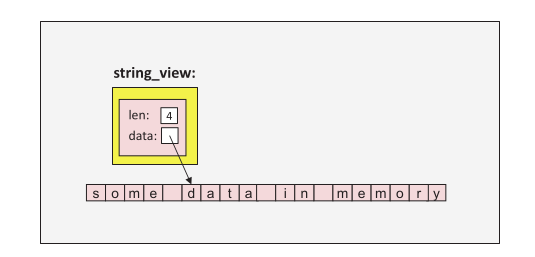
\includegraphics[scale=0.8]{../imgs/19.1.png}
        \caption{字符串视图对象}
        \label{f19.1}
    \end{center}
\end{figure}

使用字符串视图的开销很小,速度却很快(以值传递一个\texttt{string\_view}的开销总是很小)。
然而,它也有一些潜在的危险,就和原生指针一样,在使用\texttt{string\_view}时也必须
由程序员自己来保证引用的字符串序列是有效的。


\section{和\texttt{std::string}的不同之处}
和\texttt{std::string}相比,\texttt{std::string\_view}对象有以下特点:
\begin{itemize}
    \item 底层的字符序列是只读的。没有操作可以修改底层的字符。你只能赋予一个新值、
    交换值、把视图缩小为字符序列的子序列。
    \item 字符序列不保证有空字符终止。因此,字符串视图并不是一个\emph{空字符终止的字节流(NTBS)}。
    \item \texttt{data()}返回的值可能是\texttt{nullptr}。例如,当用默认构造函数初始化一个
    字符串视图之后,调用\texttt{data()}将返回\texttt{nullptr}。
    \item 没有分配器支持。
\end{itemize}
因为可能返回\texttt{nullptr},并且可能不以空字符结尾,
所以在使用\texttt{operator[]}或\texttt{data()}之前应该
总是使用\texttt{size()}获取长度
(除非你已经知道了长度)。


\section{使用字符串视图}
字符串视图有两个主要的应用:
\begin{enumerate}
    \item 你可能已经分配或者映射了字符序列或者字符串的数据,
    并且想在不分配更多内存的情况下使用这些数据。典型的例子是内存映射文件或者处理长文本的子串。
    \item 你可能想提升接收字符串为参数并以只读方式使用它们的函数/操作的性能,
    且这些函数/操作不需要结尾有空字符。

    这种情况的一种特殊形式是想以类似于\texttt{string}的API来处理字符串字面量对象:
    \begin{lstlisting}
    std::string_view hello{"hello world"};
    \end{lstlisting}
\end{enumerate}
第一个应用通常意味着只需要传递字符串视图,然而程序逻辑必须保证底层的字符序列仍然有效
(即内存映射文件不会中途取消映射)。
你也可以在任何时候使用一个字符串视图来初始化或赋值给\texttt{std::string}。

注意不要把字符串视图当作“更好的string”来使用。
这样可能导致性能问题和一些\hyperref[ch19.3.1]{运行时错误}。
请仔细的阅读下面的小节。


\section{使用字符串视图作为参数}
下面是使用字符串视图作为只读字符串的第一个例子,
这个例子定义了一个函数将传入的字符串视图作为前缀,之后打印一个集合中的元素:
\begin{lstlisting}
    #include <string_view>

    template<typename T>
    void printElems(const T& coll, std::string_view prefix = {})
    {
        for (const auto& elem : coll) {
            if (prefix.data()) {    // 排除nullptr
                std::cout << prefix << ' ';
            }
            std::cout << elem << '\n';
        }
    }
\end{lstlisting}
这里,把函数参数声明为\texttt{std::string\_view},与声明为\texttt{std::string}比较起来,
可能会减少一次分配堆内存的调用。具体的情况依赖于是否传递的是短字符串和是否使用了短字符串优化(SSO)。
例如,如果我们像下面这么声明:
\begin{lstlisting}
    template<typename T>
    void printElems(const T& coll, const std::string& prefix = {});
\end{lstlisting}
然后传递了一个字符串字面量,那么这个调用会创建一个临时的string,这将会在堆上分配一次内存,
除非使用了短字符串优化。
通过使用字符串视图,将不会分配内存,因为字符串视图只\emph{指向}字符串字面量。

注意在使用值未知的字符串视图前应该检查\texttt{data()}来排除\texttt{nullptr}。
这里为了避免写入额外的空格分隔符,必须检查\texttt{nullptr}。
值为\texttt{nullptr}的字符串视图写入到输出流时不应该写入任何字符。

另一个例子是使用字符串视图作为只读的字符串来改进\hyperref[ch15.1.1]
{\texttt{std::optional<>}章节的\texttt{asInt()}示例},
改进的方法就是把参数声明为字符串视图:\label{改进asInt}
\inputcodefile{lib/asint.cpp}
将\texttt{asInt()}的参数改为字符串视图之后需要进行很多修改。
首先,没有必要再使用\texttt{std::stoi()}来转换为整数,因为\texttt{stoi()}的参数是string,
而根据string view创建string的开销相对较高。

作为代替,我们向新的标准库函数\hyperref[ch31.2.1]{\texttt{std::from\_chars()}}传递了字符范围。
这个函数需要两个字符指针为参数,分别代表字符序列的起点和终点,并进行转换。
注意这意味着我们可以避免单独处理空字符串视图,这种情况下\texttt{data()}返回\texttt{nullptr},
\texttt{size()}返回0,因为从\texttt{nullptr}到\texttt{nullptr+0}是一个有效的空范围
(任何指针类型都支持与0相加,并且不会有任何效果)。

\texttt{std::from\_chars()}返回一个\texttt{std::from\_chars\_result}类型的结构体,
它有两个成员:一个指针\texttt{ptr}指向未被处理的第一个字符,
另一个成员\texttt{ec}的类型是\texttt{std:errc},\texttt{std::errc\{\}}代表没有错误。
因此,使用返回值中的\texttt{ec}成员初始化\texttt{ec}之后(使用了\nameref{ch1}),
下面的检查将在转换失败时返回\hyperref[nullopt]{\texttt{nullopt}}:
\begin{lstlisting}
    if (ec != std::errc{}) {
        return std::nullopt;
    }
\end{lstlisting}
使用字符串视图还可以显著\hyperref[ch22.1.2.1]{提升子字符串排序的性能}。

\subsection{字符串视图有害的一面}\label{ch19.3.1}
通常“智能对象”例如智能指针会比相应的语言特性更安全(至少不会更危险)。
因此,你可能会有一种印象:字符串视图是一种字符串的引用,应该比字符串引用更安全或者至少一样安全。
然而不幸的是,事实并不是这样的,字符串视图远比字符串引用或者智能指针更危险。
它们的行为更近似于原生字符指针。

\subsubsection{不要把临时字符串赋值给字符串视图}
考虑声明一个返回新字符串的函数:
\begin{lstlisting}
    std::string retString();
\end{lstlisting}
使用返回值总是安全的:
\begin{itemize}
    \item 用返回值来初始化一个string或者用\texttt{auto}声明的对象是安全的:
    \begin{lstlisting}
    std::string s1 = retString();   // 安全
    \end{lstlisting}
    \item 用返回值初始化常量string引用,只在局部使用时也是安全的。
    因为引用会延长返回值的生命周期:
    \begin{lstlisting}
    std::string& s2 = retString();  // 编译期ERROR(缺少const)

    const std::string& s3 = retString();  // s3延长了返回的string的生命周期
    std::cout << s3 << '\n';        // OK
    auto&& s4 = retString();        // s4延长了返回的string的生命周期
    std::cout << s4 << '\n';        // OK
    \end{lstlisting}
\end{itemize}
字符串视图没有这么安全,它\emph{既不}拷贝\emph{也不}延长返回值的生命周期:
\begin{lstlisting}
    std::string_view sv = retString(); // sv不延长返回值的生命周期
    std::cout << sv << '\n';           // 运行时ERROR:返回值已经被销毁
\end{lstlisting}
这里,在第一条语句结束时返回的字符串已经被销毁了,所以使用指向它的字符串视图\texttt{sv}
将会导致未定义的运行时错误。

这个问题类似于如下调用:
\begin{lstlisting}
    const char* p = retString().c_str();
\end{lstlisting}
或者:
\begin{lstlisting}
    auto p = retString().c_str();
\end{lstlisting}
因此,当使用返回的字符串视图时必须非常小心:
\footnote{可以在这里找到关于这个例子的讨论:
\url{https://groups.google.com/a/isocpp.org/forum/\#!topic/std-discussion/Gj5gt5E-po8}}
\begin{lstlisting}
    // 非常危险:
    std::string_view substring(const std::string& s, std::size_t idx = 0);

    // 因为:
    auto sub = substring("very nice", 5); // 返回临时string的视图
                                          // 但是临时string已经被销毁了
    std::cout << sub << '\n';     // 运行时ERROR:临时字符串s已经被销毁
\end{lstlisting}

\subsubsection{返回值类型是字符串视图时不要返回字符串}
返回值类型是字符串视图时返回字符串是非常危险的。因此,你\emph{不应该}像下面这样写:
\begin{lstlisting}
    class Person {
        std::string name;
    public:
        ...
        std::string_view getName() const {  // 不要这么做
            return name;
        }
    };
\end{lstlisting}
这是因为,下面的代码将会产生运行时错误并导致未定义行为:
\begin{lstlisting}
    Person createPerson();
    auto n = createPerson().getName();  // OOPS:delete临时字符串
    std::cout << "name: " << n << '\n'; // 运行时错误
\end{lstlisting}
如果把\texttt{getName()}改为返回一个字符串类型的值或引用就不会有这个问题了,
因为\texttt{n}将会变为返回值的拷贝。

\subsubsection{函数模板应该使用\texttt{auto}作为返回值类型}
注意无意中把字符串作为字符串视图返回是很常见的。
例如,下面的两个函数单独看起来都很有用:
\begin{lstlisting}
    // 为字符串视图定义+,返回string:
    std::string operator+ (std::string_view sv1, std::string_view sv2) {
        return std::string(sv1) + std::string(sv2);
    }

    // 泛型连接函数
    template<typename T>
    T concat (const T& x, const T& y) {
        return x + y;
    }
\end{lstlisting}
然而,如果把它们一起使用就很容易导致运行时错误:
\begin{lstlisting}
    std::string_view hi = "hi";
    auto xy = concat(hi, hi);   // xy是std::string_view
    std::cout << xy << '\n';    // 运行时错误:指向的string已经被销毁了
\end{lstlisting}
这样的代码很可能在无意中被写出来。真正的问题在于\texttt{concat()}的返回类型。
如果你把返回类型交给编译期自动推导,上面的例子将会把\texttt{xy}初始化为\texttt{std::string}:
\begin{lstlisting}
    // 改进的泛型连接函数
    template<typename T>
    auto concat (const T& x, const T& y) {
        return x + y;
    }
\end{lstlisting}

\subsubsection{不要在调用链中使用字符串视图来初始化字符串}
在一个中途或者最后需要字符串的调用链中使用字符串视图可能会适得其反。
例如,如果你定义了一个有如下构造函数的类\texttt{Person}:
\begin{lstlisting}
    class Person {
        std::string name;
    public:
        Person (std::string_view n) // 不要这样做
            : name {n} {
        }
        ...
    };
\end{lstlisting}
传递一个字符串字面量或者之后还会使用的string是没问题的:
\begin{lstlisting}
    Person p1{"Jim"};       // 没有性能开销
    std::string s = "Joe";
    Person p2{s};           // 没有性能开销
\end{lstlisting}
然而,使用move的string将会导致不必要的开销。
因为传入的string首先要隐式转换为字符串视图,
之后会再用它创建一个新的string,会再次分配内存:
\begin{lstlisting}
    Person p3{std::move(s)};  // 性能开销:move被破坏
\end{lstlisting}
不要在这里使用\texttt{std::string\_view}。以值传参然后把值move到成员里仍然是
最佳的方案(除非你想要双倍的开销):
\begin{lstlisting}
    class Person {
        std::string name;
    public:
        Person (std::string n) : name{std::move(n)} {
        }
        ...
    };
\end{lstlisting}
如果我们必须创建/初始化一个string,直接作为参数创建可以让我们在传参时享受所有可能的优化。
最后只需要简单的把参数move就行了,这个操作开销很小。

因此,如果我们使用一个返回临时字符串的辅助函数来初始化一个字符串:
\begin{lstlisting}
    std::string newName()
    {
        ...
        return std::string{...};
    }

    Person p{newName()};
\end{lstlisting}
\hyperref[ch5]{强制省略拷贝}特性将把新string的实质化过程推迟到值被传递给构造函数。
构造函数里我们有了一个叫\texttt{n}的string,这是一个有内存地址的对象
(一个\emph{广义左值(glvalue)})。之后把这个对象的值move到成员\texttt{name}里。

\subsubsection{安全使用字符串视图的总结}
总结起来就是\textbf{小心地使用\texttt{std::string\_view}},
也就是说你应该按下面这样调整你的编码风格:
\begin{itemize}
    \item 不要在那些会把参数传递给string的API中使用string view。
    \begin{itemize}
        \item 不要用string view形参来初始化string成员。
        \item 不要把string设为string view调用链的终点。
    \end{itemize}
    \item 不要返回string view。
    \begin{itemize}
        \item 除非它只是转发输入的参数,或者你可以标记它很危险,例如,通过命名来体现危险性。
    \end{itemize}
    \item \textbf{函数模板}永远不应该返回泛型参数的类型\textbf{T}。
    \begin{itemize}
        \item 作为替代,返回\texttt{auto}类型。
    \end{itemize}
    \item 永远不要用返回值来初始化string view。
    \item \textbf{不要}把返回泛型类型的函数模板的返回值赋给\textbf{\texttt{auto}}。
    \begin{itemize}
        \item 这意味着AAA(\emph{总是auto(Almost Always Auto)})原则不适用于string view。
    \end{itemize}
\end{itemize}
如果因为这些规则太过复杂或者太困难而不能遵守,那就完全不要
使用\texttt{std::string\_view}(除非你知道自己在做什么)。


\section{字符串视图类型和操作}
这一节详细描述字符串视图类型和操作

\subsection{字符串视图的具体类型}
在头文件\texttt{<string\_view>}中,C++标准库为\texttt{basic\_string\_view<>}提供了很多
特化版本:
\begin{itemize}
    \item 类\texttt{std::string\_view}是预定义的字符类型为\texttt{char}的特化模板:
    \begin{lstlisting}
    namespace std {
        using string_view = basic_string_view<char>;
    }
    \end{lstlisting}
    \item 对于使用宽字符集,例如Unicode或者某些亚洲字符集的字符串,还定义了另外三个类型:
    \begin{lstlisting}
    namespace std {
        using u16string_view = basic_string_view<char16_t>;
        using u32string_view = basic_string_view<char32_t>;
        using wstring_view = basic_string_view<wchar_t>;
    }
    \end{lstlisting}
\end{itemize}
在接下来的几节中,使用哪一种字符串视图并没有任何区别。
这几种字符串视图类的用法和问题都是一样的,因为它们都有相同的接口。
因此,“string view”意味着任何string view类型:\texttt{string\_view}、
\texttt{u16string\_view}、\texttt{u32string\_view}、\texttt{wstring\_view}。
这本书中的例子通常使用类型\texttt{string\_view},因为欧洲和英美的环境是大部分软件开发的
普遍环境。

\subsection{字符串视图的操作}
表\hyperref[t19.1]{字符串视图的操作}列出了字符串视图的所有操作。
\begin{table}[htb]
    \centering
    \begin{tabular}{l|l}
        \hline
        \textbf{操作}                        & \textbf{效果}                        \\
        \hline
        \emph{构造函数}                        & 创建或拷贝一个字符串视图                       \\
        \emph{析构函数}                        & 销毁一个字符串视图                          \\
        \texttt{=}                         & 赋予新值                               \\
        \texttt{swap()}                    & 交换两个字符串视图的值                        \\
        \texttt{==、!=、<、<=、>,>=、compare()} & 比较字符串视图                            \\
        \texttt{empty()}                   & 返回字符串视图是否为空                        \\
        \texttt{size()、length()}           & 返回字符的数量                            \\
        \texttt{max\_size()}               & 返回可能的最大字符数                         \\
        \texttt{[]、at()}                   & 访问一个字符                             \\
        \texttt{front()、back()}            & 访问第一个或最后一个字符                       \\
        \texttt{<<}                        & 将值写入输出流                            \\
        \texttt{copy()}                    & 把内容拷贝或写入到字符数组                      \\
        \texttt{data()}                    & 返回\texttt{nullptr}或常量字符数组(没有空字符终止) \\
        \emph{查找函数}                        & 查找子字符串或字符                          \\
        \texttt{begin()、end()}             & 提供普通迭代器支持                          \\
        \texttt{cbegin()、cend()}           & 提供常量迭代器支持                          \\
        \texttt{rbegin()、 rend()}          & 提供反向迭代器支持                          \\
        \texttt{crbegin()、crend()}         & 提供常量反向迭代器支持                        \\
        \texttt{substr()}                  & 返回子字符串                             \\
        \texttt{remove\_prefix()}          & 移除开头的若干字符                          \\
        \texttt{remove\_suffix()}          & 移除结尾的若干字符                          \\
        \texttt{hash<>}                    & 计算哈希值的函数对象的类型                      \\
        \hline
    \end{tabular}
    \caption{字符串视图的操作}
    \label{t19.1}
\end{table}

除了\texttt{remove\_prefix}和\texttt{remove\_suffix()}之外,
所有字符串视图的操作\texttt{std::string}也都有。
然而,相应的操作的保证可能有些许不同,\texttt{data()}的返回值可能是\texttt{nullptr}
或者没有空字符终止。

\subsubsection{构造}
你可以使用很多种方法来创建字符串视图:用默认构造函数创建、用拷贝函数构造创建、从原生字符数组创建
(空字符终止或者指明长度)、从\texttt{std::string}创建或者从带有\texttt{sv}后缀的字面量创建。
然而,注意以下几点:
\begin{itemize}
    \item 默认构造函数创建的字符串视图对象调用\texttt{data()}会返回\texttt{nullptr}。
    因此,\texttt{operator[]}调用将无效。
    \begin{lstlisting}
    std::string_view sv;
    auto p = sv.data();     // 返回nullptr
    std::cout << sv[0];     // ERROR:没有有效的字符
    \end{lstlisting}
    \item 当使用空字符终止的字节流初始化字符串视图时,最终的大小是不包括\texttt{'\textbackslash 0'}在内的
    字符的数量,另外索引空字符所在的位置是无效的:
    \begin{lstlisting}
    std::string_view sv{"hello"};
    std::cout << sv;        // OK
    std::cout << sv.size(); // 5
    std::cout << sv.at(5);  // 抛出std::out_of_range异常
    std::cout << sv[5];     // 未定义行为
    std::cout << sv.data(); // OOPS:恰好sv后边还有个'\0',所以能直接输出字符指针
    \end{lstlisting}
    你可以指定传递的字符数量来把空字符初始化为字符串视图的一部分:
    \begin{lstlisting}
    std::string_view sv{"hello", 6};    // NOTE:包含'\0'的6个字符
    std::cout << sv.size();             // 6
    std::cout << sv.at(5);              // OK,打印出'\0'的值
    std::cout << sv[5];                 // OK,打印出'\0'的值
    std::cout << sv.data();             // OK
    \end{lstlisting}
    \item 为了从一个string创建一个字符串视图,有一个为\texttt{std::string}定义的隐式转换运算符。
    再强调一次,string保证在最后一个字符之后有一个空字符,字符串视图没有这个保证:
    \begin{lstlisting}
    std::string s = "hello";
    std::cout << s.size();      // 5
    std::cout << s.at(5);       // 抛出std::out_of_range异常
    std::cout << s[5];          // OK,打印出'\0'的值
    std::cout << s.data();      // OK

    std::string_view sv{s};
    std::cout << sv.size();     // 5
    std::cout << sv.at(5);      // 抛出std::out_of_range异常
    std::cout << sv[5];         // 未定义行为
    std::cout << sv.data();     // OOPS:只有当sv后有'\0'时才能正常工作
    \end{lstlisting}
    \item 因为后缀\texttt{sv}定义了字面量运算符,所以可以像下面这样创建一个字符串视图:
    \begin{lstlisting}
    using namespace std::literals;
    auto s = "hello"sv;
    \end{lstlisting}
\end{itemize}
注意\texttt{std::char\_traits}成员被改为了\texttt{constexpr},
所以你可以在编译期用一个字符串字面量初始化字符串视图:\label{编译期字符串视图}
\begin{lstlisting}
    constexpr string_view hello = "Hello World!";
\end{lstlisting}

\subsubsection{结尾的空字符}
创建字符串视图的不同方式展示了字符串视图优越的一点,理解这一点是很重要的:
一般情况下,字符串视图的值不以空字符结尾,甚至可能是\texttt{nullptr}。
因此,你应该\textbf{总是}在访问字符串视图的字符之前检查\texttt{size()}
(除非你知道了长度)。
然而,你\emph{可能}会遇到两个特殊的场景,这两个场景会让人很迷惑:
\begin{enumerate}
    \item 你可以确保字符串视图的值以空字符结尾,尽管空字符并不是值的一部分。
    当你用字符串字面量初始化字符串视图时就会遇到这种情况:
    \begin{lstlisting}
    std::string_view sv1{"hello"};      // sv1的结尾之后有一个'\0'
    \end{lstlisting}
    这里,字符串视图的状态可能让人很困惑。这种状态有明确的定义所以可以将它用作空字符结尾的
    字符序列。然而,只有当我们明确知道这个字符串视图后有一个不属于自身的空字符时才有明确的定义。
    \item 你可以确保\texttt{'\textbackslash 0'}成为字符串视图的一部分。例如:
    \begin{lstlisting}
    std::string_view sv2{"hello", 6};   // 参数6使'\0'变为值的一部分
    \end{lstlisting}
    这里,字符串视图的状态可能让人困惑:打印它的话看起来像是只有5个字符,
    但它的实际状态是持有6个字符
    (空字符成为了值的一部分,使它变得更像一个两段的字符串(视图)(binary string(view)))。
\end{enumerate}
问题在于要想确保字符串视图后有一个空字符的话,这两种方式哪一种更好。
我倾向于不要用这两种方式中的任何一种,但截止目前,C++还没有更好的实现方式。
看起来我们似乎还需要一个既保证以空字符结尾又不需要拷贝字符
的字符串视图类型(就像\texttt{std::string}一样)。
在没有更好的替代的情况下,字符串视图就只能这么用了。
事实上,我们已经可以看到很多提案建议C++标准把返回字符指针的
函数的返回类型替换为\texttt{string\_view}
(\url{https://wg21.link/P0555r0}有一个例子)。

\subsubsection{哈希}
C++标准库保证值相同的字符串和字符串视图的哈希值相同。

\subsubsection{修改字符串视图}
这里有几个修改字符串视图的操作:
\begin{itemize}
    \item 你可以赋予新值或者交换两个字符串视图的值:
    \begin{lstlisting}
    std::string_view sv1 = "hey";
    std::string_view sv2 = "world";
    sv1.swap(sv2);
    sv2 = sv1;
    \end{lstlisting}
    \item 你可以跳过开头或结尾的字符(即把起始位置后移或者把结尾位置前移)。
    \begin{lstlisting}
    std::string_view sv = "I like my kindergarten";
    sv.remove_prefix(2);
    sv.remove_suffix(8);
    std::cout << sv;    // 打印出:like my kind
    \end{lstlisting}
\end{itemize}
注意没有对\texttt{operator+}的支持。因此:
\begin{lstlisting}
    std::string_view sv1 = "hello";
    std::string_view sv2 = "world";
    auto s1 = sv1 + sv2;    // ERROR
\end{lstlisting}
一个操作数必须是string:
\begin{lstlisting}
    auto s2 = std::string(sv1) + sv2;   // OK
\end{lstlisting}
注意字符串视图没有到string的隐式类型转换,因为这个过程需要分配内存,开销很大。
所以必须使用显式的转换。
\footnote{理论上讲,我们可以标准化一个操作来把两个字符串视图连接起来并返回新的string,
但直到目前为止还没有实现。}

\subsection{其他类型对字符串视图的支持}
理论上讲,任何需要传递字符串值的地方都可以传递字符串视图,
前提是接收者只读取值且不需要空字符结尾。

然而,到目前为止,C++标准只为大多数重要的场景添加了支持:
\begin{itemize}
    \item 使用字符串时可以联合使用字符串视图:
    \begin{itemize}
        \item 你可以从一个字符串视图创建一个string(构造函数是explicit的)。如果字符串视图
        没有值(\texttt{data()}返回\texttt{nullptr}),字符串将被初始化为空。
        \item 你可以把字符串视图用作字符串的赋值、扩展、插入、替换、比较或查找操作的参数。
        \item 存在从string到string view的隐式类型转换。
    \end{itemize}
    \item 你可以把字符串视图传给\texttt{std::quoted},它把参数用双引号括起来输出。例如:
    \begin{lstlisting}
    using namespace std::literals;

    auto s = R"(some\value)"sv;     // raw string view
    std::cout << std::quoted(s);    // 输出:"some\value"
    \end{lstlisting}
    \item 你可以使用字符串视图初始化、扩展或比较\hyperref[ch20.2.3]{文件系统路径}。
\end{itemize}
其他对字符串视图的支持,例如C++标准库中的正则表达式库的支持,仍然缺失。


\section{在API中使用字符串视图}
字符串视图开销很小并且每一个\texttt{std::string}都可以用作字符串视图。
因此,看起来好像\texttt{std::string\\
\_view}是更好的用作字符串参数的类型。然而,有一些细节很重要\ldots

首先,只有当函数按照如下约束使用参数时,使用\texttt{std::string\_view}才有意义:
\begin{itemize}
    \item 它并不需要结尾有空字符。给一个以单个\texttt{const char*}
    为参数而没有长度参数的C函数传递参数时就不属于这种情况。
    \item 它不会违反传入参数的生命周期。通常,这意味着接收函数只会在传入值的生命周期结束之前使用它。
    \item 调用者函数不应该更改底层字符的所有权(例如销毁它、改变它的值或者释放它的内存)。
    \item 它可以处理参数值为\texttt{nullptr}的情况。
\end{itemize}
注意同时有\texttt{std::string}和\texttt{std::string\_view}重载的函数可能会导致歧义:
\begin{lstlisting}
    void foo(const std::string&);
    void foo(std::string_view);

    foo("hello");   // ERROR:歧义
\end{lstlisting}
最后,记住\hyperref[ch19.3.1]{上文提到的警告}:
\begin{itemize}
    \item 不要把临时字符串赋给字符串视图。
    \footnote{译者注:此处原文是Do not assign temporary string views to strings. 应是作者笔误。}
    \item 不要返回字符串视图。
    \item 不要在调用链中使用字符串视图来初始化或重设字符串的值。
\end{itemize}
带着这些考虑,让我们来看一些使用字符串视图进行改进的例子。

\subsection{使用字符串视图代替string}
考虑下列代码:
\begin{lstlisting}
    // 带前缀输出时间点:
    void print (const std::string& prefix, const std::chrono::system_clock::time_point& tp)
    {
        // 转换为日历时间:
        auto rawtime{std::chrono::system_clock::to_time_t(tp)};
        std::string ts{std::ctime(&rawtime)};   // 注意:不是线程安全的

        ts.resize(ts.size()-1); // 跳过末尾的换行符

        std::cout << prefix << ts;
    }
\end{lstlisting}
可以被替换为下列代码:
\begin{lstlisting}
    void print (std::string_view prefix, const std::chrono::system_clock::time_point& tp)
    {
        auto rawtime{std::chrono::system_clock::to_time_t(tp)};
        std::string_view ts{std::ctime(&rawtime)};  // 注意:不是线程安全的

        ts.remove_suffix(1);    // 跳过末尾的换行符

        std::cout << prefix << ts;
    }
\end{lstlisting}
最先想到也是最简单的改进就是把只读字符串引用\texttt{prefix}换成字符串视图,
只要我们不使用会因为没有值或者没有空终止符而失败的操作就可以。
这个例子中我们只是打印字符串视图的值,这是没问题的。
如果字符串视图没有值(\texttt{data()}返回\texttt{nullptr})将不会输出任何字符。
注意字符串视图是以值传参的,因为拷贝字符串视图的开销很小。

我们也对内部\texttt{ctime()}返回的值使用了字符串视图。
然而,我们必须小心保证当我们在字符串视图中使用它时它的值还存在。
也就是说,这个值只有在下一次\texttt{ctime()}或者\texttt{asctime()}调用之前有效。
因此,在多线程环境下,这个函数将导致问题(使用string时也有一样的问题)。

如果函数返回把前缀和时间点连接起来的字符串,代码可能会像下面这样:
\begin{lstlisting}
    std::string toString (std::string_view prefix, const std::chrono::system_clock::time_point& tp)
    {
        auto rawtime{std::chrono::system_clock_to_time_t(tp)};
        std::string_view ts{std::ctime(&rawtime)};  // 注意:不是线程安全的

        ts.remove_suffix(1);    // 跳过末尾的换行符
        return std::string{prefix} + ts; // 很不幸没有两个字符串视图的+运算符
    }
\end{lstlisting}
注意我们不能简单地用\texttt{operator+}连接两个字符串视图。
我们必须把其中一个转换为\texttt{std::string}
(很不幸这个操作会分配不必要的内存)。如果字符串视图没有值
(\texttt{data()}返回\texttt{nullptr}),字符串将为空。

另一个使用字符串视图的例子是使用字符串视图和
并行算法来\hyperref[{ch22.1.2.1}]{排序子字符串}:
\begin{lstlisting}
    sort(std::execution::par, coll.begin(), coll.end(),
         // 译者注:此处原文是
         // sort(coll.begin(), coll.end(),
         // 应是作者笔误

         [] (const auto& a, const auto& b) {
             return std::string_view{a}.substr(2) < std::string_view{b}.substr(2);
         });
\end{lstlisting}
要比使用string的子字符串快得多:
\begin{lstlisting}
    sort(std::execution::par, coll.begin(), coll.end(),
         [] (const auto& a, const auto& b) {
             return a.substr(2) < b.substr(2);
         });
\end{lstlisting}
这是因为string的\texttt{substr()}函数会返回一个分配自己内存的新字符串。


\section{后记}
首个引用语义的字符串类由Jeffrey Yasskin在\url{https://wg21.link/n3334}中提出
(命名为\texttt{string\_ref})。
这个类因Jeffrey Yasskin的\url{https://wg21.link/n3921}提案
而被Library Fundamentals TS采纳。

这个类因Beman Dawes和Alisdair Meredith的\url{https://wg21.link/p0220r1}提案
而和其他组件一起被C++17标准采纳。之后为了更好的集成,Marshall Clow在
\url{https://wg21.link/p0254r2}和\url{https://wg21.link/p0403r1}中、
Nicolai Josuttis在\url{https://wg21.link/p0392r0}中添加了一些修改。

Antony Polukhin在发表于\url{https://wg21.link/p0426r1}提案中添加了对
\texttt{constexpr}的支持。

Daniel Krügler发表的\url{https://wg21.link/lwg2946}中包含了一些修复
(作为C++17的缺陷被C++20采纳)。

    \chapter{文件系统库}\label{ch20}
直到C++17,Boost.Filesystem库终于被C++标准采纳。
在这个过程中,这个库用新的语言特性进行了很多调整、改进了和其他库的一致性、
进行了精简、还扩展了很多缺失的功能(例如计算两个文件系统路径之间的相对路径)。


\section{基本的示例}
让我们以一些基本的示例开始。

\subsection{打印文件系统路径类的属性}
下面的程序允许我们传递一个字符串作为文件系统路径,然后根据给定路径的文件类型打印出一些信息:
\inputcodefile{filesystem/checkpath1.cpp}
我们首先把传入的命令行参数转换为了一个文件系统路径:
\begin{lstlisting}
    std::filesystem::path p{argv[1]};   // p代表一个文件系统路径(有可能不存在)
\end{lstlisting}
然后,我们进行了下列检查:
\begin{itemize}
    \item 如果该路径代表一个普通文件,我们打印出它的大小:
    \begin{lstlisting}
    if (is_regular_file(p)) {   // 路径p是普通文件吗?
        std::cout << p << " exists with " << file_size(p) << " bytes\n";
    }
    \end{lstlisting}
    像下面这样调用程序:
    \begin{blacklisting}
    checkpath checkpath.cpp
    \end{blacklisting}
    将会有如下输出:
    \begin{blacklisting}
    "checkpath.cpp" exists with 907 bytes
    \end{blacklisting}
    注意输出路径时会自动把路径名用双引号括起来输出
    (把路径用双引号括起来、反斜杠用另一个反斜杠转义,
    \hyperref[ch20.1.1.1]{对Windows路径来说是一个问题})。
    \item 如果路径是一个目录,我们遍历这个目录中的所有文件并打印出这些文件的路径:
    \begin{lstlisting}
    if (is_directory(p)) {      // 路径p是目录吗?
        std::cout << p << " is a directory containing:\n";
        for (auto& e : std::filesystem::directory_iterator{p}) {
            std::cout << "  " << e.path() << '\n';
        }
    }
    \end{lstlisting}
    这里,我们使用了\texttt{directory\_iterator},
    它提供了\texttt{begin()}和\texttt{end()},所以我们可以使用范围for循环来遍历
    \texttt{directory\_entry}元素。在这里,我们使用了\texttt{directory\_entry}的
    成员函数\texttt{path()},返回该目录项的文件系统路径。
    像下面这样调用程序:
    \begin{blacklisting}
    checkpath .
    \end{blacklisting}
    输出将是:
    \begin{blacklisting}
    "." is a directory containing:
    "./checkpath.cpp"
    "./checkpath.exe"
    ...
    \end{blacklisting}
    \item 最后,我们检查传入的文件系统路径是否不存在:
    \begin{lstlisting}
    if (exists(p)) {        // 路径p存在吗?
        ...
    }
    \end{lstlisting}
\end{itemize}
注意根据\emph{参数依赖查找(argument dependent lookup)(ADL)},
你不需要使用完全限定的名称来调用\texttt{is\_regular\_\\
file()}、\texttt{file\_size()}、\texttt{is\_directory()}、\texttt{exists()}等函数。
它们都属于命名空间\texttt{std::filesystem},但是因为它们的参数也属于这个命名空间,
所以调用它们时会自动在这个命名空间中进行查找。

\subsubsection{在Windows下处理路径}\label{ch20.1.1.1}
(译者注:可能是水平有限,完全看不懂作者在这一小节的逻辑,
所以只能按照自己的理解胡乱翻译,如有错误请见谅。)

默认情况下,输出路径时用双引号括起来并用反斜杠转义反斜杠在Windows
下会导致一个问题。在Windows下以如下方式调用程序:
\begin{blacklisting}
    checkpath C:\
\end{blacklisting}
将会有如下输出:
\begin{blacklisting}
    "C:\\" is a directory containing:
    ...
    "C:\\Users"
    "C:\\Windows"
\end{blacklisting}
用双引号括起来输出路径可以确保输出的文件名可以被直接复制粘贴到其他程序里,
并且经过转义之后还会恢复为原本的文件名。
然而,终端通常不接受这样的路径。

因此,一个在Windows下的可移植版本应该使用成员函数\texttt{string()},
这样可以在向标准输出写入路径时避免输出双引号:
\inputcodefile{filesystem/checkpath2.cpp}
现在,在Windows上以如下方式调用程序:
\begin{blacklisting}
    checkpath C:\
\end{blacklisting}
将会有如下输出:
\begin{blacklisting}
    "C:\" is a directory containing:
    ...
    "C:\Users"
    "C:\Windows"
\end{blacklisting}
有一些\hyperref[ch20.3.4]{其他转换}可以把路径转换为通用格式
或者把string转换为本地编码。

\subsection{用\texttt{switch}语句处理不同的文件系统类型}
我们可以像下面这样修改并改进上面的例子:
\inputcodefile{filesystem/checkpath3.cpp}

\subsubsection{命名空间\texttt{fs}}
首先,我们做了一个非常普遍的操作:我们定义了\texttt{fs}作为命名空间
\texttt{std::filesystem}的缩写:
\begin{lstlisting}
    namespace fs = std::filesystem;
\end{lstlisting}
使用这个新初始化的命名空间的一个例子是下面\texttt{switch}语句中的路径\texttt{p}:
\begin{lstlisting}
    fs::path p{argv[1]};
\end{lstlisting}
这里的\texttt{switch}语句使用了新的\nameref{ch2.2}特性,
初始化路径的同时把路径的类型作为分支条件:
\begin{lstlisting}
    switch (fs::path p{argv[1]}; status(p).type()) {
        ...
    }
\end{lstlisting}
表达式\texttt{status(p).type()}首先创建了一个\texttt{file\_status}对象,
然后该对象的\texttt{type()}方法返回了一个\texttt{file\_type}类型的值。
通过这种方式我们可以直接处理不同的类型,而不需要使用\texttt{is\_regular\_file()}、
\texttt{is\_directory()}等函数构成的if-else链。
我们通过多个步骤(先调用\texttt{status()}再调用\texttt{type()})才得到了最后的类型,
因此我们不需要为不感兴趣的其他信息付出多余的系统调用开销。

注意可能已经有特定实现的\texttt{file\_type}存在。例如,
Windows就提供了\hyperref[junction]{特殊的文件类型\texttt{junction}}。
然而,使用了它的代码是不可移植的。

\subsection{创建不同类型的文件}\label{ch20.1.3}
在介绍了文件系统的只读操作之后,让我们给出首个进行修改的例子。
下面的程序在一个子目录\texttt{tmp}中创建了不同类型的文件:
\inputcodefile{filesystem/createfiles.cpp}
让我们一步步来分析这段程序。

\subsubsection{命名空间\texttt{fs}}
首先,我们又一次定义了\texttt{fs}作为命名空间\texttt{std::filesystem}的缩写:
\begin{lstlisting}
    namespace fs = std::filesystem;
\end{lstlisting}
之后我们使用这个命名空间为临时文件创建了一个基本的子目录:
\begin{lstlisting}
    fs::path testDir{"tmp/test"};
\end{lstlisting}

\subsubsection{创建目录}
当我们尝试创建子目录时:
\begin{lstlisting}
    create_directories(testDir);
\end{lstlisting}
通过使用\texttt{create\_directories()}我们可以递归创建整个路径中所有缺少的目录
(还有一个\texttt{create\_\\
directory()}只在已存在的目录中创建目录)。

当目标目录已经存在时这个调用并不会返回错误。
然而,其他的问题会导致错误并抛出一个相应的异常。

如果\texttt{testDir}已经存在,\texttt{create\_directories()}会返回\texttt{false}。
因此,你可以这么写:
\begin{lstlisting}
    if (!create_directories(testDir)) {
        std::cout << "\"" << testDir.string() << "\" already exists\n";
    }
\end{lstlisting}

\subsubsection{创建普通文件}
之后我们用一些内容创建了一个新文件\texttt{tmp/test/data.txt}:
\begin{lstlisting}
    auto testFile = testDir / "data.txt";
    std::ofstream dataFile{testFile};
    if (!dataFile) {
        std::cerr << "OOPS, can't open \"" << testFile.string() << "\"\n";
        std::exit(EXIT_FAILURE);  // 失败退出程序
    }
    dataFile << "The answer is 42\n";
\end{lstlisting}
这里,我们使用了运算符\texttt{/}来扩展路径,然后传递给文件流的构造函数。
如你所见,普通文件的创建可以使用现有的I/O流库来实现。
然而,I/O流的构造函数多了一个以文件系统路径为参数的版本
(一些函数例如\texttt{open()}也添加了这种重载版本)。

注意你仍然应该总是检查创建/打开文件的操作是否成功了。
这里有很多种可能发生的错误(\hyperref[ch20.1.3.6]{见下文})。

\subsubsection{创建符号链接}
接下来的语句尝试创建符号链接\texttt{tmp/slink}指向目录\texttt{tmp/test}:
\begin{lstlisting}
    create_directory_symlink("test", testDir.parent_path() / "slink");
\end{lstlisting}
注意第一个参数的路径是以即将创建的符号链接所在的目录为起点的相对路径。
因此,你必须传递\texttt{"test"}而不是\texttt{"tmp/test"}来高效的
创建链接\texttt{tmp/slink}指向\texttt{tmp/test}。如果你调用:
\begin{lstlisting}
    std::filesystem::create_directory_symlink("tmp/test", "tmp/slink");
\end{lstlisting}
你将会高效的创建符号链接\texttt{tmp/slink},然而它会指向\texttt{tmp/tmp/test}。

注意通常情况下,也可以调用\texttt{create\_symlink()}代替\texttt{create\_
directory\_symlink()}来创建目录的符号链接。
然而,一些操作系统可能对目录的符号链接有特殊处理或者当知道要创建的符号链接指向目录时会有优化,
因此,当你想创建指向目录的符号链接时你应该使用\texttt{create\_directory\_symlink()}。

最后,注意这个调用在Windows上可能会失败并导致\hyperref[创建链接失败]{错误处理},
因为创建符号链接可能需要管理员权限。

\subsubsection{递归遍历目录}\label{ch20.1.3.5}
最后,我们递归地遍历了当前目录:
\begin{lstlisting}
    auto iterOpts = fs::directory_options::follow_directory_symlink;
    for (auto& e : fs::recursive_directory_iterator(".", iterOpts)) {
        std::cout << "  " << e.path().lexically_normal().string() << '\n';
    }
\end{lstlisting}
注意我们使用了一个递归目录迭代器并传递了选项\texttt{follow\_directory\_symlink}来
遍历符号链接。因此,我们在POSIX兼容系统上可能会得到类似于如下输出:
\begin{blacklisting}
    /home/nico:
    ...
    tmp
    tmp/slink
    tmp/slink/data.txt
    tmp/test
    tmp/test/data.txt
    ...
\end{blacklisting}
在Windows系统上有类似如下输出:
\begin{blacklisting}
    C:\Users\nico:
    ...
    tmp
    tmp\slink
    tmp\slink\data.txt
    tmp\test
    tmp\test\data.txt
    ...
\end{blacklisting}
注意在我们打印目录项之前调用了\texttt{lexically\_normal()}。
如果略过这一步,目录项的路径可能会包含一个前缀,
这个前缀是创建目录迭代器时传递的实参。
因此,在循环内直接打印路径:
\begin{lstlisting}
    auto iterOpts = fs::directory_options::follow_directory_symlink;
    for (auto& e : fs::recursive_directory_iterator(".", iterOpts)) {
        std::cout << "  " << e.path() << '\n';
    }
\end{lstlisting}
将会在POSIX兼容系统上有如下输出:
\begin{blacklisting}
    all files:
    ...
    "./testdir"
    "./testdir/data.txt"
    "./tmp"
    "./tmp/test"
    "./tmp/test/data.txt"
\end{blacklisting}
在Windows上,输出将是:
\begin{blacklisting}
    all files:
    ...
    ".\\testdir"
    ".\\testdir\\data.txt"
    ".\\tmp"
    ".\\tmp\\test"
    ".\\tmp\\test\\data.txt"
\end{blacklisting}
通过调用\texttt{lexically\_normal()}我们可以得到正规化的路径,
它移除了前导的代表当前路径的点。还有,\hyperref[ch20.1.1.1]{如上文所述},
通过调用\texttt{string()}我们避免了输出路径时用双引号括起来。
这里没有调用\texttt{string()}的输出结果在POSIX兼容的系统上看起来OK(只是路径两端有双引号),
但在Windows上的结果看起来就很奇怪(因为每一个反斜杠都需要反斜杠转义)。

\subsubsection{错误处理}\label{ch20.1.3.6}
文件系统往往是麻烦的根源。你可能因为在文件名中使用了无效的字符而导致操作失败,
或者当你正在访问文件系统时它已经被其他程序修改了。
因此,根据平台和权限的不同,这个程序中可能会有很多问题。

对于那些没有被返回值覆盖的情况(例如当目录已经存在时),
我们捕获了相应的异常并打印了一般的信息和第一个路径:
\begin{lstlisting}
    try {
        ...
    }
    catch (const fs::filesystem_error& e) {
        std::cerr << "EXCEPTION: " << e.what() << '\n';
        std::cerr << "    path1: \"" << e.path1().string() << "\"\n";
    }
\end{lstlisting}
例如,如果我们不能创建目录,将会打印出类似于如下消息:
\begin{blacklisting}
    EXCEPTION: filesystem error: cannot create directory: [tmp/test]
    path1: "tmp/test"
\end{blacklisting}
如果我们不能创建符号链接可能是因为它已经存在了,
或者我们可能需要特殊权限,这些情况下你可能会得到如下消息:\label{创建链接失败}
\begin{blacklisting}
    EXCEPTION: create_directory_symlink: Can't create a file when it already exists:
                                         "tmp\test\data.txt", "testdir"
        path1: "tmp\test\data.txt"
\end{blacklisting}
或者:
\begin{blacklisting}
    EXCEPTION: create_directory_symlink: A requied privilege is not held by the
                                         client.: "test", "tmp\slink"
        path1: "test"
\end{blacklisting}
在每一种情况下,都要注意在多用户/多进程操作系统中情况可能会在任何时候改变,
这意味着你刚刚创建的目录甚至可能已经被删除、重命名、或已经被同名的文件覆盖。
因此,很显然不能只根据当前的情况就保证一个预期操作一定是有效的。
最好的方式就是尝试做想做的操作(例如,创建目录、打开文件)
并处理抛出的异常和错误,或者验证预期的行为。

然而,有些时候文件系统操作能正常执行但不是按你预想的结果。
例如,如果你想在指定目录中创建一个文件并且已经有了一个和目录同名的指向另一个目录的符号链接,
那么这个文件可能在一个预料之外的地方创建或者覆写。
\footnote{译者注:比如你想在当前目录下递归创建\texttt{"a/b"},
但已经有了一个\texttt{"a"}是一个指向\texttt{"c"}目录的符号链接,
这时你实际会在目录\texttt{"c"}下创建\texttt{"b"}。}
这种情况是有可能的(用户完全有可能会创建目录的符号链接),但是如果你想检测这种情况,
在创建文件之前你需要\nameref{ch20.4.1.1}(这可能比你一开始想的要复杂很多)。

再强调一次:文件系统并不保证进行处理之前的检查的结果直到你进行处理时仍然有效。

\subsection{使用并行算法处理文件系统}
参见\hyperref[ch22.6.1.4]{dirsize.cpp}查看另一个使用并行算法计算目录树中所有文件大小之和的例子。


\section{原则和术语}
在讨论文件系统库的细节之前,我们不得不继续介绍一些设计原则和术语。
这是必须的,因为标准库要覆盖不同的操作系统并把系统提供的接口映射为公共的API。

\subsection{通用的可移植的分隔符}
C++标准库不仅标准化了所有操作系统的文件系统中公共的部分,在很多情况下,
C++标准还尽可能的遵循POSIX标准的要求来实现。
对于一些操作,只要是合理的就应该能正确执行,如果操作是不合理的,实现应该报错。
这些错误可能是:
\begin{itemize}
    \item 特殊的字符不能被用作文件名
    \item 创建了文件系统不支持的元素(例如,符号链接)
\end{itemize}
不同文件系统的差异也应该纳入考虑:
\begin{itemize}
    \item 大小写敏感:\\
    \texttt{"hello.txt"}和\texttt{"Hello.txt"}和\texttt{"hello.TXT"}可能指向
    同一个文件(Windows上)也可能指向三个不同的文件(POSIX兼容系统)。
    \item 绝对路径和相对路径:\\
    在某些系统上,\texttt{"/bin"}是一个绝对路径(POSIX兼容系统),
    然而在某些系统上不是(Windows)。
\end{itemize}

\subsection{命名空间}
文件系统库在\texttt{std}里有自己的子命名空间\texttt{filesystem}。
一个很常见的操作是定义缩写\texttt{fs}:
\begin{lstlisting}
    namespace fs = std::filesystem;
\end{lstlisting}
这允许我们使用\texttt{fs::current\_path()}代
替\texttt{std::filesystem::current\_path()}。

这一章的示例代码中将经常使用\texttt{fs}作为缩写。

注意你应该总是使用完全限定的函数调用,尽管不指明命名空间时
通过\emph{参数依赖查找(argument dependent lookup)(ADL)}也能够工作。
但如果不用命名空间限定有时可能\hyperref[ADL导致意外行为]{导致意外的行为}。

\subsection{文件系统路径}\label{ch20.2.3}
文件系统库的一个关键元素是\texttt{path}。它代表文件系统中某一个文件的位置。
它由可选的根名称、可选的根目录、和一些以目录分隔符分隔的文件名组成。
路径可以是相对的(此时文件的位置依赖于当前的工作目录)或者是绝对的。

路径可能有不同的格式:
\begin{itemize}
    \item 通用格式,这是可移植的
    \item 本地格式,这是底层文件系统特定的
\end{itemize}
在POSIX兼容系统上通用格式和本地格式没有什么区别。
在Windows上,通用格式\texttt{/tmp/test.txt}也是有效的本地格式,
另外\texttt{\textbackslash tmp\textbackslash test.txt}也是有效的
(\texttt{/tmp/test.txt}和\texttt{\textbackslash tmp\textbackslash test.txt}
是同一个路径的两种本地版本)。在OPenVMS上,相应的本地格式将是\texttt{[tmp]test.txt}。

也有一些特殊的文件名:
\begin{itemize}
    \item \texttt{"."}代表当前目录
    \item \texttt{".."}代表父目录
\end{itemize}
通用的路径格式如下:\\
\hspace*{2em}\texttt{[rootname] [rootdir] [relativepath]}\\
这里:
\begin{itemize}
    \item 可选的根名称是实现特定的(例如,在POSIX系统上可以是\texttt{//host},
    而在Windows上可以是\texttt{C:})
    \item 可选的根目录是一个目录分隔符
    \item 相对路径是若干目录分隔符分隔的文件名
\end{itemize}
目录分隔符由一个或多个\texttt{'/'}组成或者是实现特定的。

可移植的通用路径的例子有:
\begin{blacklisting}
    //host1/bin/hello.txt
    .
    tmp/
    /a/b//.../c
\end{blacklisting}
注意在POSIX系统上最后一个路径和\texttt{/a/c}指向同一个位置,并且都是绝对路径。
而在Windows上则是相对路径(因为没有指定驱动器/分区(盘))。

另一方面,\texttt{C:/bin}在Windows上是绝对路径(在\texttt{"C"}盘上的根目录\texttt{"bin"}),
但在POSIX系统上是一个相对路径(目录\texttt{"C:"}下的子目录\texttt{"bin"})。

在Windows系统上,反斜杠是实现特定的目录分隔符,
因此上面的路径\emph{也}可以使用反斜杠作为目录分隔符:
\begin{blacklisting}
    \\host1\bin\hello.txt
    .
    tmp\
    \a\b\..\c
\end{blacklisting}
文件系统库提供了\hyperref[ch20.3.4]{在本地格式和通用格式之间转换的函数}。

一个\texttt{path}可能为空,这意味着没有定义路径。
这种状态的含义\emph{不}需要和\texttt{"."}一样。它的含义依赖于上下文。

\subsection{正规化}
路径可以进行正规化,在正规化的路径中:
\begin{itemize}
    \item 文件名由单个推荐的目录分隔符分隔。
    \item 除非整个路径就是\texttt{"."}(代表当前目录),否则路径中不会使用\texttt{"."}。
    \item 路径中除了开头以外的地方不会包含\texttt{".."}(不能在路径中上下徘徊)。
    \item 除非整个路径就是\texttt{"."}或者\texttt{".."},否则当路径结尾的文件名是目录时要在最后加上目录分隔符。
\end{itemize}
注意正规化之后以目录分隔符结尾的路径和不以目录分隔符结尾的路径是不同的。
这是因为在某些操作系统中,当它们知道目标路径是一个目录时行为可能会发生改变
(例如,有尾部的分隔符时符号链接将被解析)。

表\hyperref[t20.1]{路径正规化的效果}列举了一些在POSIX系统和Windows系统上
对路径进行正规化的例子。注意再重复一次,在POSIX系统上,\texttt{C:bar}和\texttt{C:}只是
把冒号作为文件名的一部分的单个文件名,并没有特殊的含义,而在Windows上,它们指定了一个分区。
\begin{table}[htb]
    \centering
    \begin{tabular}{l|l|l}
        \hline
        \textbf{路径}                                    & \textbf{POSIX正规化}                              & \textbf{Windows正规化}                                               \\
        \hline
        \texttt{foo/.///bar/../}                       & \texttt{foo/}                                  & \texttt{foo\textbackslash}                                        \\
        \texttt{//host/../foo.txt}                     & \texttt{//host/foo.txt}                        & \texttt{\textbackslash \textbackslash host\textbackslash foo.txt} \\
        \texttt{./f/../.f/}                            & \texttt{.f/}                                   & \texttt{.f\textbackslash}                                         \\
        \texttt{C:bar/../}                             & \texttt{.}                                     & \texttt{C:}                                                       \\
        \texttt{C:/bar/..}                             & \texttt{C:/}                                   & \texttt{C:\textbackslash}                                         \\
        \texttt{C:\textbackslash bar\textbackslash ..} & \texttt{C:\textbackslash bar\textbackslash ..} & \texttt{C:\textbackslash}                                         \\
        \texttt{/./../data.txt}                        & \texttt{/data.txt}                             & \texttt{\textbackslash data.txt}                                  \\
        \texttt{././}                                  & \texttt{.}                                     & \texttt{.}                                                        \\
        \hline
    \end{tabular}
    \caption{路径正规化的效果}
    \label{t20.1}
\end{table}

注意路径\texttt{C:\textbackslash bar\textbackslash ..}在POSIX兼容系统上经过正规化
之后没有任何变化。原因是这些系统上反斜杠并不是目录分隔符,所以这整个路径只是一个
带有冒号、两个反斜杠、两个点的\emph{单个}文件名。

文件系统库同时提供了\hyperref[ch20.3.3]{词法正规化}(不访问文件系统)
和\hyperref[ch20.4.5]{依赖文件系统的正规化}两种方式的相关函数。

\subsection{成员函数VS独立函数}
文件系统库提供了一些函数,有些是成员函数有些是独立函数。这么做的目的是:
\begin{itemize}
    \item \textbf{成员函数开销较小}。这是因为它们是纯词法的操作,并不会访问实际的文件系统,
    这意味着它们不需要进行操作系统调用。例如:
    \begin{lstlisting}
    mypath.is_absolute()        // 检查路径是否是绝对的
    \end{lstlisting}
    \item \textbf{独立函数开销较大}。因为它们通常会访问实际的文件系统,
    这意味着需要进行操作系统调用。例如:
    \begin{lstlisting}
    equivalent(path1, path2);   // 如果两个路径指向同一个文件则返回true
    \end{lstlisting}
\end{itemize}
有时,文件系统库甚至为同一个功能既提供根据词法的版本又提供访问实际文件系统的版本:
\begin{lstlisting}
    std::filesystem::path fromP, toP;
    ...
    toP.lexically_relative(fromP);  // 返回从fromP到toP的词法路径
    relative(toP, fromP);           // 返回从fromP到toP的实际路径
\end{lstlisting}
得益于\emph{参数依赖查找(ADL)},很多情况下当调用独立函数时你不需要指明完整命名空间
\texttt{std::filesystem},只要参数是文件系统库里定义的类型。只有当用其它类型隐式转换
为参数时你才需要给出完全限定的函数名。例如:\label{ADL导致意外行为}
\begin{lstlisting}
    create_directory(std::filesystem::path{"tmpdir"});  // OK
    remove(std::filesystem::path{"tmpdir"});            // OK
    std::filesystem::create_directory("tmpdir");        // OK
    std::filesystem::remove("tmpdir");                  // OK
    create_directory("tmpdir");                         // ERROR
\end{lstlisting}
最后一个调用将会编译失败,因为我们并没有传递文件系统命名空间里的类型作为参数,
因此也不会在该命名空间里查找符号\texttt{create\_directory}。

然而,这里有一个著名的陷阱:
\begin{lstlisting}
    remove("tmpdir");   // OOPS:调用C函数remove()
\end{lstlisting}
根据你包含的头文件,这个调用可能会找到C函数\texttt{remove()},
它的行为有一些不同:它也会删除指定的文件但不会删除空目录。

因此,强烈推荐使用完全限定的文件系统库里的函数名。例如:
\begin{lstlisting}
    namespace fs = std::filesystem;
    ...
    fs::remove("tmpdir");   // OK:调用C++文件系统库函数remove()
\end{lstlisting}

\subsection{错误处理}
\hyperref[ch20.1.3.6]{如上文所述},文件系统是错误的根源。
你必须考虑相应的文件是否存在、文件操作是否被允许、该操作是否会违背资源限制。
另外,当程序运行时其它进程可能创建、修改、或者移除了某些文件,这意味着事先检查
并不能保证没有错误。

问题在于从理论上讲,你不能提前保证下一次文件系统操作能够成功。
任何事先检查的结果都可能在你实际进行处理时失效。
因此,最好的方法是在进行一个或多个文件系统操作时处理好相应的异常或者错误。

注意,当读写普通文件时,默认情况下I/O流并不会抛出异常或错误。
当操作遇到错误时它只会什么也不做。因此,建议至少检查一下文件是否被成功打开。

因为并不是所有情况下都适合抛出异常(例如当一个文件系统调用失败时你想直接处理),
所以文件系统库使用了混合的异常处理方式:
\begin{itemize}
    \item 默认情况下,文件系统错误会作为异常处理。
    \item 然而,如果你想的话可以在本地处理具体的某一个错误。
\end{itemize}
因此,文件系统库通常为每个操作提供两个重载版本:
\begin{enumerate}
    \item 默认情况下(没有额外的错误处理参数),出现错误时抛出\texttt{filesystem\_error}异常。
    \item 传递额外的输出参数时,可以得到一个错误码或错误信息,而不是异常。
\end{enumerate}
注意在第二种情况下,你可能会得到一个特殊的返回值来表示特定的错误。

\subsubsection{使用\texttt{filesystem\_error}异常}\label{ch20.2.6.1}
例如,你可以尝试像下面这样创建一个目录:
\begin{lstlisting}
    if (!create_directory(p)) { // 发生错误时抛出异常(除非错误是该路径已经存在)
        std::cout << p << " already exists\n";  // 该路径已经存在
    }
\end{lstlisting}
这里没有传递错误码参数,因此错误时通常会抛出异常。
然而,注意当目录已存在时这种特殊情况是直接返回\texttt{false}。
因此,只有当其他错误例如没有权限创建目录、路径\texttt{p}无效、
违反了文件系统限制(例如路径长度超过上限)时才会抛出异常。

可以直接或间接的用\texttt{try-catch}包含这段代码,
然后处理\texttt{std::filesystem::filesystem\_error}异常:
\begin{lstlisting}
    try {
        ...
        if (!create_directory(p)) { // 错误时抛出异常(除非错误是该路径已经存在)
            std::cout << p << " already exists\n"; // 该路径已经存在
        }
        ...
    }
    catch (const std::filesystem::filesystem_error& e) { // 派生自std::exception
        std::cout << "EXCEPTION: " << e.what() << '\n';
        std::cout << "     path: " << e.path1() << '\n';
    }
\end{lstlisting}
如你所见,文件系统异常提供了标准异常的\texttt{what()}函数API来返回一个
实现特定的错误信息。然而,API还提供了\texttt{path1()}来获取错误相关的第一个路径,
和\texttt{path2()}来获取相关的第二个路径。

\subsubsection{使用\texttt{error\_code}参数}\label{ch20.2.6.2}
另一种创建目录的方式如下所示:
\begin{lstlisting}
    std::error_code ec;
    create_directory(p, ec);    // 发生错误时设置错误码
    if (ec) {                   // 如果设置了错误码(因为发生了错误)
        std::cout << "ERROR: " << ec.message() << "\n";
    }
\end{lstlisting}
之后,我们还可以检查特定的错误码:
\begin{lstlisting}
    if (ec == std::errc::read_only_file_system) {   // 如果设置了特定的错误码
        std::cout << "ERROR: " << p << " is read-only\n";
    }
\end{lstlisting}
注意这种情况下,我们仍然必须检查\texttt{create\_directory()的返回值}:
\begin{lstlisting}
    std::error_code ec;
    if (!create_directory(p, ec)) { // 发生错误时设置错误码
        // 发生任何错误时
        std::cout << "can't create directory " << p << "\n";
        std::cout << "error: " << ec.message() << "\n";
    }
\end{lstlisting}
然而,并不是所有的文件系统操作都提供这种能力(因为它们在正常情况下会返回一些值)。

类型\texttt{error\_code}由C++11引入,它包含了一系列可移植的错误条件,例如
\texttt{std::errc::read\_only\_\\
filesystem}。在POSIX兼容的系统上这些被映射为\texttt{errno}的值。

\subsection{文件类型}\label{ch20.2.7}
不同的操作系统支持不同的文件类型。标准文件系统库中也考虑到了这一点,它定义了一个
枚举类型\texttt{file\_type},标准中定义了如下的值:
\begin{lstlisting}
    namespace std::filesystem {
        enum class file_type {
            regular, directory, symlink,
            block, character, fifo, socket,
            ...
            none, not_found, unknown,
        };
    }
\end{lstlisting}
表\hyperref[t20.2]{\texttt{file\_type}的值}列出了这些值的含义。
\begin{table}[htb]
    \centering
    \begin{tabular}{l|l}
        \hline
        \textbf{值}          & \textbf{含义}   \\
        \hline
        \texttt{regular}    & 普通文件          \\
        \texttt{directory}  & 目录文件          \\
        \texttt{symlink}    & 符号链接文件        \\
        \texttt{character}  & 字符特殊文件        \\
        \texttt{block}      & 块特殊文件         \\
        \texttt{fifo}       & FIFO或者管道文件    \\
        \texttt{socket}     & 套接字文件         \\
        \ldots              & 附加的实现定义的文件类型  \\
        \texttt{none}       & 文件的类型未知       \\
        \texttt{unknown}    & 文件存在但推断不出类型   \\
        \texttt{not\_found} & 虚拟的表示文件不存在的类型 \\
        \hline
    \end{tabular}
    \caption{文件系统类型的值}
    \label{t20.2}
\end{table}

操作系统平台可能会提供附加的文件类型值。然而,使用它们是不可移植的。
例如,Windows就提供了文件类型值\texttt{junction},它被用于NTFS文件系统中的
\emph{NTFS junctions}(也被称为软链接)。
它们被用作链接来访问同一台电脑上不同的子卷(盘)。\label{junction}

除了普通文件和目录之外,最常见的类型是符号链接,它是一种指向另一个位置的文件。
指向的位置可能有一个文件也可能没有。
注意有些操作系统和/或文件系统(例如FAT文件系统)完全不支持符号链接。
有些操作系统只支持普通文件的符号链接。
注意在Windows上需要特殊的权限才能创建符号链接,可以用\texttt{mklink}命令创建。

字符特殊文件、块特殊文件、FIFO、套接字都来自于UNIX文件系统。
目前,Visual C++并没有使用这四种类型中的任何一个。
\footnote{Windows管道的行为有些不同,也不被识别为\texttt{fifo}。}

如你所见,有一些特殊的值来表示文件不存在或者类型未知或者无法探测出类型。

在这一章的剩余部分我将使用两种广义的类型来代表相应的若干文件类型:\label{文件类型}
\begin{itemize}
    \item \emph{其他文件}:除了普通文件、目录、符号链接之外的所有类型的文件。
    库函数\texttt{is\_other()}和这个术语相匹配。
    \item \emph{特殊文件}:下列类型的文件:字符特殊文件、块特殊文件、FIFO、套接字。
\end{itemize}
另外,\emph{特殊文件}类型加上实现定义的文件类型就构成了\emph{其他文件}类型。


\section{路径操作}
有很多处理文件系统的操作。这些操作涉及的关键类型是\texttt{std::filesystem::path},
它表示一个可能存在也可能不存在的文件的绝对或相对的路径。

你可以创建路径、检查路径、修改路径、比较路径。
因为这些操作一般都不会访问实际的文件系统(例如不会检查文件是否存在,也不会解析符号链接),
所以它们的开销很小。因此,它们通常被定义为成员函数(如果这些操作既不是构造函数也不是运算符的话)。

\subsection{创建路径}
表\hyperref[t20.3]{创建路径}列出了创建新的路径对象的方法。
\begin{table}[htb]
    \centering
    \begin{tabular}{l|l}
        \hline
        \textbf{调用}                      & \textbf{效果}      \\
        \hline
        \texttt{path\{charseq\}}         & 用一个字符序列初始化路径     \\
        \texttt{path\{beg, end\}}        & 用一个范围初始化路径       \\
        \texttt{u8path(u8string)}        & 用一个UTF-8字符串初始化路径 \\
        \texttt{current\_path()}         & 返回当前工作目录的路径      \\
        \texttt{temp\_directory\_path()} & 返回临时文件的路径        \\
        \hline
    \end{tabular}
    \caption{创建路径}
    \label{t20.3}
\end{table}

第一个构造函数以字符序列为参数,这里的字符序列代表一系列有效的方式:
\begin{itemize}
    \item 一个\texttt{string}
    \item 一个\texttt{string\_view}
    \item 一个以空字符结尾的字符数组
    \item 一个以空字符结尾的字符输入迭代器(指针)
\end{itemize}
注意\texttt{current\_path()}和\texttt{temp\_directory\_path()}都是开销较大的操作,
因为它们依赖于系统调用。如果给\texttt{current\_path()}传递一个参数,它也可以用来
\hyperref[ch20.4.6]{修改当前工作目录}。

通过\texttt{u8path()}你可以使用UTF-8字符串创建可移植的路径。例如:
\begin{lstlisting}
    // 将路径p初始化为"Köln"(Cologne的德语名):
    std::filesystem::path p{std::filesystem::u8path(u8"K\u00F6ln")};
    ...

    // 用UTF-8字符串创建目录:
    std::string utf8String = readUTF8String(...);
    create_directory(std::filesystem::u8path(utf8String));
\end{lstlisting}

\subsection{检查路径}\label{ch20.3.2}
表\hyperref[t20.4]{检查路径}列出了检查路径\texttt{p}时可以调用的函数。
注意这些操作都不会访问底层的操作系统,因此都是\texttt{path}类的成员函数。
\begin{table}[htb]
    \centering
    \begin{tabular}{l|l}
        \hline
        \textbf{调用}                       & \textbf{效果}                 \\
        \hline
        \texttt{p.empty()}                & 返回路径是否为空                    \\
        \texttt{p.is\_absolute()}         & 返回路径是否是绝对的                  \\
        \texttt{p.is\_relative()}         & 返回路径是否是相对的                  \\
        \texttt{p.has\_filename()}        & 返回路径是否既不是目录也不是根名称           \\
        \texttt{p.has\_stem()}            & 和\texttt{has\_filename()}一样 \\
        \texttt{p.has\_extension()}       & 返回路径是否有扩展名                  \\
        \texttt{p.has\_root\_name()}      & 返回路径是否包含根名称                 \\
        \texttt{p.has\_root\_directory()} & 返回路径是否包含根目录                 \\
        \texttt{p.has\_root\_path()}      & 返回路径是否包含根名称或根目录             \\
        \texttt{p.has\_parent\_path()}    & 返回路径是否包含父路径                 \\
        \texttt{p.has\_relative\_path()}  & 返回路径是否不止包含根元素               \\
        \texttt{p.filename()}             & 返回文件名(或者空路径)                \\
        \texttt{p.stem()}                 & 返回没有扩展名的文件名(或者空路径)          \\
        \texttt{p.extension()}            & 返回扩展名(或者空路径)                \\
        \texttt{p.root\_name()}           & 返回根名称(或者空路径)                \\
        \texttt{p.root\_directory()}      & 返回根目录(或者空路径)                \\
        \texttt{p.root\_path()}           & 返回根元素(或者空路径)                \\
        \texttt{p.parent\_path()}         & 返回父路径(或者空路径)                \\
        \texttt{p.relative\_path()}       & 返回不带根元素的路径(或者空路径)           \\
        \texttt{p.begin()}                & 返回路径元素的起点                   \\
        \texttt{p.end()}                  & 返回路径元素的终点                   \\
        \hline
    \end{tabular}
    \caption{检查路径}
    \label{t20.4}
\end{table}

每一个路径要么是绝对的要么是相对的。如果没有根目录那么路径就是相对的
(相对路径也可能包含根名称;例如,\texttt{C:hello.txt}就是Windows下的一个相对路径)。

\texttt{has\_...()}函数等价于检查相应的没有\texttt{has\_}前缀的函数的返回值是否为空路径。

注意下面几点:
\begin{itemize}
    \item 如果路径含有根元素或者目录分隔符那么就包含父路径。如果路径只由根元素组成
    (也就是说相对路径为空),\texttt{parent\_path()}的返回值就是整个路径。
    也就是说,路径\texttt{"/"}的父路径还是\texttt{"/"}。只有纯文件名的路径例如
    \texttt{"hello.txt"}的父路径是空。
    \item 如果一个路径包含文件名那么一定包含stem(文件名中不带扩展名的部分)。
    \footnote{从C++17才开始这样,因为以前文件名可以只包含扩展名。}
    \item 空路径是相对路径(除了\texttt{empty()}和\texttt{is\_relative()}
    之外的操作都返回\texttt{false}或者空路径)。
\end{itemize}
这些操作的结果可能会依赖于操作系统。例如,路径
\texttt{C:/hello.txt}
\begin{itemize}
    \item 在Unix系统上
    \begin{itemize}
        \item 是相对路径
        \item 没有根元素(既没有根名称也没有根目录),因为\texttt{C:}只是一个文件名
        \item 有父路径\texttt{C:}
        \item 有相对路径\texttt{C:/hello.txt}
    \end{itemize}
    \item 在Windows系统上
    \begin{itemize}
        \item 是绝对的
        \item 有根名称\texttt{C:}和根目录\texttt{/}
        \item 沒有父路径
        \item 有相对路径\texttt{hello.txt}
    \end{itemize}
\end{itemize}

\subsubsection{遍历路径}
你可以遍历一个路径,这将会返回路径的所有元素:根名称(如果有的话)、根目录(如果有的话)、
所有的文件名。如果路径以目录分隔符结尾,最后的元素将是空文件名。
\footnote{在C++17之前,文件系统库使用\texttt{.}来表示结尾的目录分隔符。
更改这个行为是为了区分以路径分隔符结尾的路径和以路径分隔符后还有一个点结尾的路径。}

路径迭代器是双向迭代器,所以你可以递减它。迭代器的值的类型是\texttt{path}。
然而,两个在同一个路径上迭代的迭代器可能\emph{不}指向同一个\texttt{path}对象,
即使它们迭代到了相同的路径元素。

例如,考虑:
\begin{lstlisting}
    void printPath(const std::filesystem::path& p)
    {
        std::cout << "path elements of \"" << p.string() << "\":\n";
        for (std::filesystem::path elem : p) {
            std::cout << "  \"" << elem.string() << '"';
        }
        std::cout << '\n';
    }
\end{lstlisting}
和如下代码效果相同:
\begin{lstlisting}
    void printPath(const std::filesystem::path& p)
    {
        std::cout << "path elements of \"" << p.string() << "\":\n";
        for (auto pos = p.begin(); pos != p.end(); ++pos) {
            std::filesystem::path elem = *pos;
            std::cout << "  \"" << elem.string() << '"';
        }
        std::cout << '\n';
    }
\end{lstlisting}
如果像下面这样调用这个函数:
\begin{lstlisting}
    printPath("../sub/file.txt");
    printPath("/usr/tmp/test/dir/");
    printPath("C:\\usr\\tmp\\test\\dir\\");
\end{lstlisting}
在POSIX兼容系统上的输出将会是:
\begin{blacklisting}
    path elements of "../sub/file.txt":
    ".."  "sub"  "file.txt"
    path elements of "/usr/tmp/test/dir/":
    "/"  "usr"  "tmp"  "test"  "dir"  ""
    path elements of "C:\\usr\\tmp\\test\\dir\\":
    "C:\\usr\\tmp\\test\\dir\\"
\end{blacklisting}
注意最后一个路径只是一个文件名,因为在POSIX兼容系统上\texttt{C:}不是有效的根名称,
反斜杠也不是有效的目录分隔符。

在Windows上的输出将是:
\begin{blacklisting}
    path elements of "../sub/file.txt":
    ".."  "sub"  "file.txt"
    path elements of "/usr/tmp/test/dir/":
    "/"  "usr"  "tmp"  "test"  "dir"  ""
    path elements of "C:\usr\tmp\test\dir\":
    "C:"  "\"  "usr"  "tmp"  "test"  "dir"  ""
\end{blacklisting}
为了检查路径\texttt{p}是否以目录分隔符结尾,你可以这么写:
\begin{lstlisting}
    if (!p.empty() && (--p.end())->empty()) {
        std::cout << p << " has a trailing separator\n";
    }
\end{lstlisting}

\subsection{路径I/O和转换}\label{ch20.3.3}
表\hyperref[t20.5]{路径I/O和转换}列出了路径的读写操作和转换操作。
这些函数也不会访问实际的文件系统。如果必须要处理符号链接,
你可能需要使用\hyperref[ch20.4.5]{依赖文件系统的路径转换}。
\begin{table}[htb]
    \centering
    \begin{tabular}{l|l}
        \hline
        \textbf{调用}                         & \textbf{效果}                                     \\
        \hline
        \texttt{strm << p}                  & 用双引号括起来输出路径                                     \\
        \texttt{strm >> p}                  & 读取用双引号括起来的路径                                    \\
        \texttt{p.string()}                 & 以\texttt{std::string}返回路径                       \\
        \texttt{p.wstring()}                & 以\texttt{std::wstring}返回路径                      \\
        \texttt{p.u8string()}               & 以类型为\texttt{std::u8string}的UTF-8字符串返回路径         \\
        \texttt{p.u16string()}              & 以类型为\texttt{std::u16string}的UTF-16字符串返回路径       \\
        \texttt{p.u32string()}              & 以类型为\texttt{std::u32string}的UTF-32字符串返回路径       \\
        \texttt{p.string<...>()}            & 以\texttt{std::basic\_string<...>}返回路径           \\
        \texttt{p.lexically\_normal()}      & 返回正规化的路径                                        \\
        \texttt{p.lexically\_relative(p2)}  & 返回从\texttt{p2}到\texttt{p}的相对路径(如果没有则返回空路径)      \\
        \texttt{p.lexically\_proximate(p2)} & 返回从\texttt{p2}到\texttt{p}的路径(如果没有则返回\texttt{p}) \\
        \hline
    \end{tabular}
    \caption{路径I/O和转换}
    \label{t20.5}
\end{table}

\texttt{lexically\_...()}函数会返回一个新的路径,而其他的转换函数将返回相应的字符串类型。
所有这些函数都不会修改调用者的路径。

例如,下面的代码:
\begin{lstlisting}
    std::filesystem::path p{"/dir/./sub//sub1/../sub2"};
    std::cout <<  "path:               " << p << '\n';
    std::cout <<  "string():           " << p.string() << '\n';
    std::wcout << "wstring():          " << p.wstring() << '\n';
    std::cout <<  "lexically_normal(): " << p.lexically_normal() << '\n';
\end{lstlisting}
前三行的输出是相同的:
\begin{blacklisting}
    path:               "/dir/./sub//sub1/../sub2"
    string():           /dir/./sub//sub1/../sub2
    wstring():          /dir/./sub//sub1/../sub2
\end{blacklisting}
但最后一行的输出就依赖于目录分隔符了。在POSIX兼容系统上输出是:
\begin{blacklisting}
    lexically_normal(): "/dir/sub/sub2"
\end{blacklisting}
而在Windows上输出是:
\begin{blacklisting}
    lexically_normal(): "\\dir\\sub\\sub2"
\end{blacklisting}

\subsubsection{路径I/O}
首先,注意I/O运算符以双引号括起来的字符串方式读写路径。
你可以把它们转换为字符串来避免双引号:
\begin{lstlisting}
    std::filesystem::path file{"test.txt"};
    std::cout << file << '\n';          // 输出:"test.txt"
    std::cout << file.string() << '\n'; // 输出:test.txt
\end{lstlisting}
在Windows上,情况可能会更糟糕。下面的代码:
\begin{lstlisting}
    std::filesystem::path tmp{"C:\\Windows\\Temp"};
    std::cout << tmp << '\n';
    std::cout << tmp.string() << '\n';
    std::cout << '"' << tmp.string() << "\"\n";
\end{lstlisting}
将会有如下输出:
\begin{blacklisting}
    "C:\\Windows\\Temp"
    C:\Windows\Temp
    "C:\Windows\Temp"
\end{blacklisting}
注意读取路径时既支持带双引号的字符串也支持不带双引号的字符串。
因此,所有的输出形式都能使用输入运算符再读取回来:
\begin{lstlisting}
    std::filesystem::path tmp;
    std::cin >> tmp;    // 读取有双引号和无双引号的路径
\end{lstlisting}

\subsubsection{正规化}
当你处理可移植代码时正规化可能会导致更多令人惊奇的结果。例如:
\begin{lstlisting}
    std::filesystem::path p2{"//host\\dir/sub\\/./\\"};
    // 译者注:此处原文是
    // std::filesystem::path p2{"//dir\\subdir/subsubdir\\/./\\"};
    // 应是作者笔误

    std::cout << "p2:                 " << p2 << '\n';
    std::cout << "lexically_normal(): " << p2.lexically_normal() << '\n';
\end{lstlisting}
在Windows系统上可能会有如下输出:
\begin{blacklisting}
    p2:                 "//host\\dir/sub\\/./\\"
    lexically_normal(): "\\\\host\\dir\\sub\\"
\end{blacklisting}
然而,在POSIX兼容系统上,输出将是:
\begin{blacklisting}
    p2:                 "//host\\dir/sub\\/./\\"
    lexically_normal(): "/host\\dir/sub\\/\\"
\end{blacklisting}
原因是对于POSIX兼容系统来说反斜杠既不是路径分隔符也不是有效的根名称,
这意味着我们得到了一个有三个文件名的绝对路径,三个文件名分别是\texttt{host\textbackslash dir}、
\texttt{sub\textbackslash}、\texttt{\textbackslash}。
在POSIX兼容系统上,没有办法把反斜杠作为目录分隔符处理
(\hyperref[ch20.3.4]{\texttt{generic\_string()}和\texttt{make\_preferred()}}也没有用)。
因此,对于可移植的代码,当处理路径时你应该总是使用通用路径格式。

但是,当\hyperref[遍历.]{遍历当前目录}时使用\texttt{lexically\_normal()}
移除开头的点是个好方法。

\subsubsection{相对路径}
\texttt{lexically\_relative()}和\texttt{lexically\_proximate()}都可以被用来计算
两个路径间的相对路径。不同之处在于如果没有相对路径时的行为,
只有当一个是相对路径一个是绝对路径或者两个路径的根名称不同时才会发生这种情况。
这种情况下:
\begin{itemize}
    \item 对于\texttt{p.lexically\_relative(p2)},如果没有从\texttt{p2}到\texttt{p}
    的相对路径,将会返回空路径。
    \item 对于\texttt{p.lexically\_proximate(p2)},如果没有从\texttt{p2}到\texttt{p}
    的相对路径,将会返回\texttt{p}。
\end{itemize}
因为这两个操作都是词法操作,所以不会考虑实际的文件系统(可能会有符号链接)和\texttt{current\_path()}。
如果两个路径相同,相对路径将是\texttt{"."}。例如:
\begin{lstlisting}
    fs::path{"/a/d"}.lexically_relative("/a/b/c");      // "../../d"
    fs::path{"/a/b/c"}.lexically_relative("/a/d");      // "../b/c"
    fs::path{"/a/b"}.lexically_relative("/a/b");        // "."
    fs::path{"/a/b"}.lexically_relative("/a/b/");       // "."
    fs::path{"/a/b"}.lexically_relative("/a/b\\");      // "."
    fs::path{"/a/b"}.lexically_relative("/a/d/../c");   // "../b"
    fs::path{"a/d/../b"}.lexically_relative("a/c");     // "../d/../b"
    fs::path{"a//d/..//b"}.lexically_relative("a/c");   // "../d/../b"
\end{lstlisting}
在Windows平台上,则是:
\begin{lstlisting}
    fs::path{"C:/a/b"}.lexically_relative("c:/c/d");    // ""
    fs::path{"C:/a/b"}.lexically_relative("D:/c/d");    // ""
    fs::path{"C:/a/b"}.lexically_proximate("D:/c/d");   // "C:/a/b"
\end{lstlisting}

\subsubsection{转换为字符串}
通过\texttt{u8string()}你可以将路径用作UTF-8字符串,
这是当前存储数据的通用格式。例如:
\begin{lstlisting}
    // 把路径存储为UTF-8字符串:
    std::vector<std::string> utf8paths; // 自从C++20起将改为std::u8string
    for (const auto& entry : fs::directory_iterator(p)) {
        utf8paths.push_back(entry.path().u8string());
    }
\end{lstlisting}
注意自从C++20起\texttt{u8string()}的返回值可能会从\texttt{std::string}改为
\texttt{std::u8string()}(新的UTF-8字符串类型和存储UTF-8字符
的\texttt{char8\_t}类型的提案见\url{https://wg21.link/p0482})。
\footnote{感谢Tom Honermann指出这一点,并做出这个改进(C++开始提供真正的UTF-8支持是非常重要的)。}

成员模板\texttt{string<>()}可以用来转换成特殊的字符串类型,例如一个大小写无关的字符串类型:
\begin{lstlisting}
    struct ignoreCaseTraits : public std::char_traits<char> {
        // 大小写不敏感的比较两个字符:
        static bool eq(const char& c1, const char& c2) {
            return std::toupper(c1) == std::toupper(c2);
        }
        static bool lt(const char& c1, const char& c2) {
            return std::toupper(c1) < std::toupper(c2);
        }
        // 比较s1和s2的至多前n个字符:
        static int compare(const char* s1, const char* s2, std::size_t n);
        // 在s中搜索字符c:
        static const char* find(const char* s, std::size_t n, const char& c);
    };

    // 定义一个这种类型的字符串:
    using icstring = std::basic_string<char, ignoreCaseTraits>;

    std::filesystem::path p{"/dir\\subdir/subsubdir\\/./\\"};
    icstring s2 = p.string<char, ignoreCaseTraits>();
\end{lstlisting}
注意你\emph{不}应该使用函数\texttt{c\_str()},因为它会转换为\emph{本地}字符串格式,
可能是\texttt{wchar\_t},因此你需要使用\texttt{std::wcout}代替\texttt{std::cout}
来输出到输出流。

\subsection{本地和通用格式的转换}\label{ch20.3.4}
表\hyperref[t20.6]{本地和通用格式的转换}列出了在\hyperref[ch20.2.3]{通用路径格式}和
实际平台特定实现的格式之间转换的方法。
\begin{table}[htb]
    \centering
    \begin{tabular}{l|l}
        \hline
        \textbf{调用}                       & \textbf{效果}                                    \\
        \hline
        \texttt{p.generic\_string()}      & 返回\texttt{std::string}类型的通用路径                  \\
        \texttt{p.generic\_wstring()}     & 返回\texttt{std::wstring}类型的通用路径                 \\
        \texttt{p.generic\_u8string()}    & 返回\texttt{std::u8string}类型的通用路径                \\
        \texttt{p.generic\_u16string()}   & 返回\texttt{std::u16string}类型的通用路径               \\
        \texttt{p.generic\_u32string()}   & 返回\texttt{std::u32string}类型的通用路径               \\
        \texttt{p.generic\_string<...>()} & 返回\texttt{std::basic\_string<...>()}类型的通用路径    \\
        \texttt{p.native()}               & 返回\texttt{path::string\_type}类型的本地路径格式         \\
        \emph{到本地路径的转换}                   & 到本地字符串类型的隐式转换                                  \\
        \texttt{p.c\_str()}               & 返回本地字符串格式的字符序列形式的路径                            \\
        \texttt{p.make\_preferred()}      & 把\texttt{p}中的目录分隔符替换为本地格式的分隔符并返回修改后的\texttt{p} \\
        \hline
    \end{tabular}
    \caption{本地和通用格式的转换}
    \label{t20.6}
\end{table}

这些函数在POSIX兼容系统上没有效果,因为这些系统的本地格式和通用格式没有区别。
在其他平台上调用这些函数可能会有效果:
\begin{itemize}
    \item \texttt{generic...()}函数返回转换为\hyperref[ch20.2.3]{通用格式}之后的相应类型的字符串。
    \item \texttt{native()}返回用本地字符串编码的路径,其类型为\texttt{std::filesystem::path::string\_type}。
    这个类型在Windows下是\texttt{std::wstring},这意味着你需要使用\texttt{std::wcout}
    代替\texttt{std::cout}来输出。新的重载允许我们向文件流传递本地字符串。
    \item \texttt{c\_str()}以空字符结尾的字符序列形式返回结果。注意使用这个函数是不可移植的,
    因为使用\texttt{std::cout}打印字符序列在Windows上的输出不正确。你应该使用\texttt{std::wcout}。
    \item \texttt{make\_preferred()}会使用本地的目录分隔符替换除了根名称之外的所有的目录分隔符。
    注意这是唯一一个会修改调用者的函数。因此,严格来讲,这个函数应该属于下一节的修改路径的函数,
    但因为它可以处理本地格式的转换,所以也在这里列出。
\end{itemize}
例如,在Windows上,下列代码:
\begin{lstlisting}
    std::filesystem::path p{"/dir\\subdir/subsubdir\\/./\\"};
    std::cout <<  "p:                  " << p << '\n';
    std::cout <<  "string():           " << p.string() << '\n';
    std::wcout << "wstring():          " << p.wstring() << '\n';
    std::cout <<  "lexically_normal(): " << p.lexically_normal() << '\n';
    std::cout <<  "generic_string():   " << p.generic_string() << '\n';
    std::wcout << "generic_wstring():  " << p.generic_wstring() << '\n';
    // 因为这是在Windows下,相应的本地字符串类型是wstring:
    std::wcout << "native():           " << p.native() << '\n'; // Windows!
    std::wcout << "c_str():            " << p.c_str() << '\n';
    std::cout <<  "make_preferred():   " << p.make_preferred() << '\n';
    std::cout <<  "p:                  " << p << '\n';
\end{lstlisting}
将会有如下输出:
\begin{blacklisting}
    p:                  "/dir\\subdir/subsubdir\\/./\\"
    string():           /dir\subdir/subsubdir\/./\
    wstring():          /dir\subdir/subsubdir\/./\
    lexically_normal(): "\\dir\\subdir\\subsubdir\\"
    generic_string():   /dir/subdir/subsubdir//.//
    generic_wstring():  /dir/subdir/subsubdir//.//
    native():           /dir\subdir/subsubdir\/./\
    c_str():            /dir\subdir/subsubdir\/./\
    make_preferred():   "\\dir\\subdir\\subsubdir\\\\.\\\\"
    p:                  "\\dir\\subdir\\subsubdir\\\\.\\\\"
\end{blacklisting}
再次注意:
\begin{itemize}
    \item 本地字符串格式是不可移植的。在Windows上是\texttt{wstring},而在POSIX兼容系统上是\texttt{string},
    这意味着你要使用\texttt{cout}而不是\texttt{wcout}来打印\texttt{native()}的结果。
    \item 只有\texttt{make\_preferred()}会修改调用者。其他的调用都会保持\texttt{p}不变。
\end{itemize}

\subsection{修改路径}\label{ch20.3.5}
表\hyperref[t20.7]{修改路径}列出了可以直接修改路径的操作。
\begin{table}[htb]
    \centering
    \begin{tabular}{l|l}
        \hline
        \textbf{调用}                         & \textbf{效果}                                            \\
        \hline
        \texttt{p = p2}                     & 赋予一个新路径                                                \\
        \texttt{p = sv}                     & 赋予一个字符串(视图)作为新路径                                       \\
        \texttt{p.assign(p2)}               & 赋予一个新路径                                                \\
        \texttt{p.assign(sv)}               & 赋予一个字符串(视图)作为新路径                                       \\
        \texttt{p.assign(beg, end)}         & 赋予从\texttt{beg}到\texttt{end}的元素组成的路径                   \\
        \texttt{p1 / p2}                    & 返回把\texttt{p2}作为子路径附加到\texttt{p1}之后的结果                 \\
        \texttt{p /= sub}                   & 把\texttt{sub}作为子路径附加到路径\texttt{p}之后                    \\
        \texttt{p.append(sub)}              & 把\texttt{sub}作为子路径附加到路径\texttt{p}之后                    \\
        \texttt{p.append(beg, end)}         & 把从\texttt{beg}到\texttt{end}之间的元素作为子路径附加到路径\texttt{p}之后 \\
        \texttt{p += str}                   & 把\texttt{str}里的字符添加到路径\texttt{p}之后                     \\
        \texttt{p.concat(str)}              & 把\texttt{str}里的字符添加到路径\texttt{p}之后                     \\
        \texttt{p.concat(beg, end)}         & 把从\texttt{beg}到\texttt{end}之间的元素附加到路径\texttt{p}之后      \\
        \texttt{p.remove\_filename()}       & 移除路径末尾的文件名                                             \\
        \texttt{p.replace\_filename(repl)}  & 替换末尾的文件名(如果有的话)                                        \\
        \texttt{p.replace\_extension()}     & 移除末尾的文件的扩展名                                            \\
        \texttt{p.replace\_extension(repl)} & 替换末尾的文件的扩展名(如果有的话)                                     \\
        \texttt{p.clear()}                  & 清空路径                                                   \\
        \texttt{p.swap(p2)}                 & 交换两个路径                                                 \\
        \texttt{swap(p1, p2)}               & 交换两个路径                                                 \\
        \texttt{p.make\_preferred()}        & 把\texttt{p}中的目录分隔符替换为本地格式的分隔符并返回修改后的\texttt{p}         \\
        \hline
    \end{tabular}
    \caption{修改路径}
    \label{t20.7}
\end{table}

注意\texttt{+=}和\texttt{concat()}简单的把字符添加到路径后,\texttt{/}、\texttt{/=}、
\texttt{append()}则是在路径后用目录分隔符添加一个子路径:
\begin{lstlisting}
    std::filesystem::path p{"myfile"};
    p += ".git";        // p:myfile.git
    p /= ".git";        // p:myfile.git/.git
    p.concat("1");      // p:myfile.git/.git1
    p.append("1");      // P:myfile.git/.git1/1
    std::cout << p << '\n';
    std::cout << p / p << '\n';
\end{lstlisting}
在POSIX兼容系统上输出将是:
\begin{blacklisting}
    "myfile.git/.git1/1"
    "myfile.git/.git1/1/myfile.git/.git1/1"
\end{blacklisting}
在Windows系统上输出将是:
\begin{blacklisting}
    "myfile.git\\.git1\\1"
    "myfile.git\\.git1\\1\\myfile.git\\.git1\\1"
\end{blacklisting}
注意如果添加一个绝对路径子路径意味着替换原本的路径。例如,如下操作之后:
\begin{lstlisting}
    namespace fs = std::filesystem;
    auto p1 = fs::path("/usr") / "tmp";     // 路径是/usr/tmp或者/usr\tmp
    auto p2 = fs::path("/usr/") / "tmp";    // 路径是/usr/tmp
    auto p3 = fs::path("/usr") / "/tmp";    // 路径是/tmp
    auto p4 = fs::path("/usr/") / "/tmp";   // 路径是/tmp
\end{lstlisting}
我们有了四个指向两个不同文件的路径:
\begin{itemize}
    \item \texttt{p1}和\texttt{p2}相等,都指向文件\texttt{/usr/tmp}(注意在Windows上
    它们相等,但\texttt{p1}将是\texttt{/usr\textbackslash tmp})。
    \item \texttt{p3}和\texttt{p4}相等,指向文件\texttt{/tmp},因为附加的子路径是绝对路径。
\end{itemize}
对于根元素,是否赋予新的根元素的结果将不同。例如,在Windows上,结果将是:
\begin{lstlisting}
    auto p1 = fs::path("usr") / "C:/tmp";   // 路径是C:/tmp
    auto p2 = fs::path("usr") / "C:";       // 路径是C:
    auto p3 = fs::path("C:") / "":          // 路径是C:
    auto p4 = fs::path("C:usr") / "/tmp";   // 路径是C:/tmp
    auto p5 = fs::path("C:usr") / "C:tmp";  // 路径是C:usr\tmp
    auto p6 = fs::path("C:usr") / "c:tmp";  // 路径是c:tmp
    auto p7 = fs::path("C:usr") / "D:tmp";  // 路径是D:tmp
\end{lstlisting}
函数\texttt{make\_preferred()}把一个路径内的目录分隔符替换成本地格式。
例如:
\begin{lstlisting}
    std::filesystem::path p{"//server/dir//subdir///file.txt"};
    p.make_preferred();
    std::cout << p << '\n';
\end{lstlisting}
在POSIX兼容系统上输出将是:
\begin{blacklisting}
    "//server/dir/subdir/file.txt"
\end{blacklisting}
在Windows系统上输出将是:
\begin{blacklisting}
    "\\\\server\\dir\\\\subdir\\\\\\file.txt"
\end{blacklisting}
注意开头的根名称没有被修改,因为它由两个斜杠或者反斜杠组成。
也注意这个函数在POSIX兼容系统上也不会把反斜杠转换成斜杠,因为反斜杠不被识别为目录分隔符。

\texttt{replace\_extension()}可以替换、添加、或者删除扩展名:
\begin{itemize}
    \item 如果文件已经有扩展名了,它会进行替换。
    \item 如果文件没有扩展名,会添加新的扩展名。
    \item 如果你跳过了新的扩展名参数或者新扩展名参数为空,它会移除已有的扩展名。
\end{itemize}
替换时是否有前导的点没有影响。函数会确保文件名和扩展名之间有且只有一个点。例如:
\begin{lstlisting}
    fs::path{"file.txt"}.replace_extension("tmp")   // file.tmp
    fs::path{"file.txt"}.replace_extension(".tmp")  // file.tmp
    fs::path{"file.txt"}.replace_extension("")      // file
    fs::path{"file.txt"}.replace_extension()        // file
    fs::path{"dir"}.replace_extension("tmp")        // dir.tmp
    fs::path{".git"}.replace_extension("tmp")       // .git.tmp
\end{lstlisting}
注意“纯扩展名”的文件名(例如\texttt{.git})不会被当作扩展名。
\footnote{自从C++17起才改成这样。在C++17之前,最后一条语句的结果将是\texttt{.tmp}。}

\subsection{比较路径}\label{ch20.3.6}
表\hyperref[t20.8]{比较路径}列出了可以比较两个路径的操作。
\begin{table}[htb]
    \centering
    \begin{tabular}{l|l}
        \hline
        \textbf{调用}                 & \textbf{效果}                                    \\
        \hline
        \texttt{p1 == p2}           & 返回两个路径是否相等                                     \\
        \texttt{p1 != p2}           & 返回两个路径是否不相等                                    \\
        \texttt{p1 < p2}            & 返回一个路径是否小于另一个                                  \\
        \texttt{p1 <= p2}           & 返回一个路径是否小于等于另一个                                \\
        \texttt{p1 >= p2}           & 返回一个路径是否大于等于另一个                                \\
        \texttt{p1 > p2}            & 返回一个路径是否大于另一个                                  \\
        \texttt{p.compare(p2)}      & 返回\texttt{p}是小于、等于还是大于\texttt{p2}              \\
        \texttt{p.compare(sv)}      & 返回\texttt{p}是小于、等于还是大于字符串(视图)\texttt{sv}转换成的路径 \\
        \texttt{equivalent(p1, p2)} & 访问实际文件系统的开销较大的比较操作                             \\
        \hline
    \end{tabular}
    \caption{比较路径}
    \label{t20.8}
\end{table}

注意这些比较操作大部分都不会访问实际的文件系统,这意味着它们只是以词法的方式比较,
这样开销很小但可能会导致令人惊奇的结果:
\begin{itemize}
    \item 使用\texttt{==}、\texttt{!=}、\texttt{compare()}的结果是下面的路径都不相同:
    \begin{blacklisting}
    tmp1/f
    ./tmp1/f
    tmp1/./f
    tmp1/tmp11/../f
    \end{blacklisting}
    \item 只有当分隔符以外的部分都相同时才会判定为相同。
    因此,下面的路径是相等的(假设反斜杠也是有效的目录分隔符):
    \begin{blacklisting}
    tmp1/f
    tmp1//f
    tmp1\f
    tmp1/\/f
    \end{blacklisting}
\end{itemize}
如果你使用了\texttt{lexically\_normal()}那么上面的所有路径都相等
(假设反斜杠也是有效的目录分隔符)。例如:
\begin{lstlisting}
    std::filesystem::path p1{"tmp1/f"};
    std::filesystem::path p2{"./tmp1/f"};

    p1 == p2                                                // false
    p1.compare(p2)                                          // 非0
    p1.lexically_normal() == p2.lexically_normal()          // true
    p1.lexically_normal().compare(p2.lexically_normal())    // 0
\end{lstlisting}
如果你想要访问实际的文件系统来正确处理包含符号链接的情况,你需要使用\texttt{equivalent()}。
然而,注意这个函数要求两个路径都代表已经存在的文件。
因此,一个通用的尽可能精确(但没有最佳的性能)的比较两个路径的方法是:
\begin{lstlisting}
    bool pathsAreEqual(const std::filesystem::path& p1,
                       const std::filesystem::path& p2)
    {
        return exists(p1) && exists(p2) ? equivalent(p1, p2)
            : p1.lexically_normal() == p2.lexically_normal();
    }
\end{lstlisting}

\subsection{其他路径操作}
表\hyperref[t20.9]{其他路径操作}列出了剩余的路径操作。
\begin{table}[htb]
    \centering
    \begin{tabular}{l|l}
        \hline
        \textbf{调用}              & \textbf{效果} \\
        \hline
        \texttt{p.hash\_value()} & 返回一个路径的哈希值  \\
        \hline
    \end{tabular}
    \caption{其他路径操作}
    \label{t20.9}
\end{table}

注意只有\hyperref[ch20.3.6]{相等的路径}才保证有相同的哈希值,下面的路径返回不同的哈希值:
\begin{blacklisting}
    tmp1/f
    ./tmp1/f
    tmp1/./f
    tmp1/tmp11/../f
\end{blacklisting}
因此,在把它们放入哈希表之前,你可能需要先对路径进行正规化。


\section{文件系统操作}
这一节介绍开销更大的会访问实际文件系统的操作。

因为这些操作通常会访问文件系统(要确定文件是否存在、解析符号链接等等),
它们比纯路径操作的开销要大的多。因此,它们通常是独立函数。

\subsection{文件属性}\label{ch20.4.1}
对于一个路径你可以查询很多文件属性。首先,表\hyperref[t20.10]{文件类型操作}列出了
可以检查路径\texttt{p}是否指向特定的文件并查询它的类型(如果有的话)的操作。
注意这些操作都会访问实际的文件系统,也都是独立函数。
\begin{table}[htb]
    \centering
    \begin{tabular}{l|l}
        \hline
        \textbf{调用}                     & \textbf{效果}                        \\
        \hline
        \texttt{exists(p)}              & 返回是否存在一个可访问到的文件                    \\
        \texttt{is\_symlink(p)}         & 返回是否文件\texttt{p}存在并且是符号链接          \\
        \texttt{is\_regular\_file(p)}   & 返回是否文件\texttt{p}存在并且是普通文件          \\
        \texttt{is\_directory(p)}       & 返回是否文件\texttt{p}存在并且是目录            \\
        \texttt{is\_other(p)}           & 返回是否文件\texttt{p}存在并且不是普通文件或目录或符号链接 \\
        \texttt{is\_block\_file(p)}     & 返回是否文件\texttt{p}存在并且是块特殊文件         \\
        \texttt{is\_character\_file(p)} & 返回是否文件\texttt{p}存在并且是字符特殊文件        \\
        \texttt{is\_fifo(p)}            & 返回是否文件\texttt{p}存在并且是FIFO或者管道文件    \\
        \texttt{is\_socket(p)}          & 返回是否文件\texttt{p}存在并且是套接字           \\
        \hline
    \end{tabular}
    \caption{文件类型操作}
    \label{t20.10}
\end{table}

文件系统类型的函数和相应的\hyperref[ch20.2.7]{\texttt{file\_type}值}相对应。
然而,注意这些函数(除了\texttt{is\_symlink()}之外)都会解析符号链接。也就是说,
对于一个指向目录的符号链接,\texttt{is\_symlink()}和\texttt{is\_directory()}都返回\texttt{true}。

还要注意对于\hyperref[文件类型]{特殊文件}(非普通文件、非目录、非符号链接)的检查,
根据\hyperref[文件类型]{其他文件类型}的定义,\texttt{is\_other()}会返回\texttt{true}。

对于实现特定的文件类型没有明确的便捷函数,这意味着只有\texttt{is\_other()}会返回
\texttt{true}(如果是一个指向这种文件的符号链接,那么\texttt{is\_symlink()}也会返回\texttt{true})。
你可以使用\hyperref[ch20.4.2]{文件状态API}来检测这些特定的类型。

如果不想解析符号链接,可以像下面将要讨论的\texttt{exists()}一样使用\hyperref[t20.12]{\texttt{symlink\_status()}},
并对返回的\hyperref[ch20.4.2]{\texttt{file\_status}}调用这些函数。

\subsubsection{检查文件是否存在}\label{ch20.4.1.1}
\texttt{exists()}检查是否有一个可以打开的文件。像之前讨论的一样,它会解析符号链接。
因此,对于指向不存在文件的符号链接它会返回\texttt{false}。

因此,下面的代码不能像预期中工作:
\begin{lstlisting}
    // 如果不存在文件p,创建一个符号链接p指向file:
    if (!exists(p)) {   // OOPS:检查文件p指向的目标是否不存在
        std::filesystem::create_symlink(file, p);
    }
\end{lstlisting}
如果\texttt{p}已经存在并且是一个指向不存在文件的符号链接,
\texttt{create\_symlink()}将会尝试在\texttt{p}位置处创建新的符号链接,
这会导致抛出一个相应的异常。

因为多用户/多进程操作系统中文件系统的状况可能会在任意时刻改变,最佳的方法就是尝试进行操作
并在失败时处理错误。因此,我们可以直接进行操作并\hyperref[ch20.2.6.1]{处理相应的异常}或者
传递额外的参数来\hyperref[ch20.2.6.2]{处理错误码}。

然而,有时你必须检测文件是否存在(在进行文件系统操作之前)。
例如,如果你想在指定位置创建一个文件并且该位置处已经有了一个符号链接,
那么新创建的文件(可能)会在一个意料之外的地方创建或者覆盖。
这种情况下,你应该像下面这样检查文件是否存在:
\footnote{感谢Billy O’Neal指出这一点。}
\begin{lstlisting}
    if (!exists(symlink_status(p))) {   // OK:检查p是否还不存在(作为符号链接)
        ...
    }
\end{lstlisting}
这里,我们使用了\hyperref[t20.12]{\texttt{symlink\_status()}},
它会在\emph{不}解析符号链接的情况下返回文件状态,以检查位置\texttt{p}处是否有任何文件存在。

\subsubsection{其他文件属性}
表\hyperref[t20.11]{文件属性操作}列出了一些检查额外文件属性的独立函数。
\begin{table}[htb]
    \centering
    \begin{tabular}{l|l}
        \hline
        \textbf{调用}                   & \textbf{效果}   \\
        \hline
        \texttt{is\_empty()}          & 返回文件是否为空      \\
        \texttt{file\_size()}         & 返回文件大小        \\
        \texttt{hard\_link\_count(p)} & 返回硬链接数量       \\
        \texttt{last\_write\_time(p)} & 返回最后一次修改文件的时间 \\
        \hline
    \end{tabular}
    \caption{文件属性操作}
    \label{t20.11}
\end{table}

注意路径是否为空和路径指向的文件是否为空是不同的:
\begin{lstlisting}
    p.empty()       // 如果路径p为空则返回true(开销很小)
    is_empty(p)     // 如果路径p处的文件为空返回true(文件系统操作)
\end{lstlisting}
如果文件存在并且是普通文件,那么\texttt{file\_size(p)}以字节为单位返回文件\texttt{p}的大小
(在POSIX系统上,这个值和\texttt{stat()}返回的\texttt{st\_size}成员的值相同)。
对于所有其他文件,结果是实现特定的,因此不可移植。

\texttt{hard\_link\_count(p)}返回文件系统中某一个文件存在的次数。
通常情况下,这个数字是1,但是在某些文件系统上同一个文件可以出现在不同的位置(也就是有多个不同的路径)。
这和软链接指向其他文件不同,这里的路径可以直接访问文件。只有当最后一个硬链接被删除时文件才会被删除。

\subsubsection{处理最后修改的时间}\label{ch20.4.1.3}
\texttt{last\_write\_time(p)}返回文件最后一次修改或者写入的时间。
返回的类型是标准\texttt{chrono}库里的时间点类型\texttt{time\_point}:
\begin{lstlisting}
    namespace std::filesystem {
        using file_time_type = chrono::time_point<travialClock>;
    }
\end{lstlisting}
时钟类型\emph{trivialClock}是一个实现特定的时钟类型,它能反应时钟的精度和范围。
例如,你可以这么使用它:
\begin{lstlisting}
    void printFileTime(const std::filesystem::path& p)
    {
        auto filetime = last_write_time(p);
        auto diff = std::filesystem::file_time_type::clock::now() - filetime;
        std::cout << p << " is "
                  << std::chrono::duration_cast<std::chrono::seconds>(diff).count()
                  << " Seconds old.\n";
    }
\end{lstlisting}
输出可能是:
\begin{blacklisting}
    "fileattr.cpp" is 4 Seconds old.
\end{blacklisting}
这个例子中,你可以使用:
\begin{lstlisting}
    decltype(filetime)::clock::now()
\end{lstlisting}
来代替
\begin{lstlisting}
    std::filesystem::file_time_type::clock::now()
\end{lstlisting}
注意文件系统时间点使用的时钟不保证是标准的\texttt{system\_clock}。
因此,现在还没有把文件系统时间点转换为\texttt{time\_t}然后在字符串或者输出中用作绝对时间的标准化支持。
\footnote{C++20中引入的\texttt{clock\_cast}将修复这个问题。}
然而还是有一些解决方法的,下面的代码“粗略地”把任何时钟的时间点转换为\texttt{time\_t}对象:
\begin{lstlisting}
    template<typename TimePoint>
    std::time_t toTimeT(TimePoint tp)
    {
        using system_clock = std::chrono::system_clock;
        return system_clock::to_time_t(system_clock::now() + (tp - decltype(tp)::clock::now()));
    }
\end{lstlisting}
技巧是计算出文件系统时间点和现在的差值,类型是\texttt{duration},然后加上现在的系统时钟的时间
就可以得到用系统时钟表示的文件系统时间点。这个函数不是很精确,因为不同的时钟可能有不同的精度,
而且两次\texttt{now()}调用之间可能时间差。然而,一般来说,这个函数工作得很好。

例如,对一个路径\texttt{p}我们可以调用:
\begin{lstlisting}
    auto ftime = last_write_time(p);
    std::time_t t = toTimeT(ftime);
    // 转换为日历时间(跳过末尾的换行符):
    std::string ts = ctime(&t);
    ts.resize(ts.size()-1);
    std::cout << "last access of " << p << ": " << ts << '\n';
\end{lstlisting}
输出可能是:
\begin{blacklisting}
    last access of "fileattr.exe": Sun Jun 24 10:41:12 2018
\end{blacklisting}
为了把时间格式化为我们想要的格式,我们可以这样调用:
\begin{lstlisting}
    std::time_t t = toTimeT(ftime);
    char mbstr[100];
    if (std::strftime(mbstr, sizeof(mbstr), "last access: %B %d, %Y at %H:%M\n",
                      std::localtime(&t))) {
        std::cout << mbstr;
    }
\end{lstlisting}
输出可能是:
\begin{blacklisting}
    last access: June 24, 2018 at 10:41
\end{blacklisting}
把任意文件系统时间点转换为字符串的一个有用的辅助函数可以是:
\inputcodefile{filesystem/ftimeAsString.hpp}
注意\texttt{ctime()}和\texttt{strftime()}是非线程安全的,不能在并发环境中使用。

参见\nameref{ch20.4.4.2}小节查看相应的修改最后访问时间的API。

\subsection{文件状态}\label{ch20.4.2}
为了避免文件系统访问,有一个特殊的类型\texttt{file\_status}可以被用来存储并修改
被缓存的文件类型和权限。发生以下情况时可以设置状态:
\begin{itemize}
    \item 当使用表\hyperref[t20.12]{文件状态的操作}中的方法访问某个指定路径的文件状态时
    \item 当\nameref{ch20.5}时
\end{itemize}
\begin{table}[htb]
    \centering
    \begin{tabular}{l|l}
        \hline
        \textbf{调用}                 & \textbf{效果}                                   \\
        \hline
        \texttt{status(p)}          & 返回文件\texttt{p}的\texttt{file\_status}(解析符号链接)  \\
        \texttt{symlink\_status(p)} & 返回文件\texttt{p}的\texttt{file\_status}(不解析符号链接) \\
        \hline
    \end{tabular}
    \caption{文件状态的操作}
    \label{t20.12}
\end{table}
不同之处在于路径\texttt{p}是否解析符号链接,\texttt{status()}将会解析符号链接
并返回指向的文件的属性(文件状态也可能是没有文件),而\texttt{symlink\_status(p)}
将会返回符号链接自身的状态。

表\hyperref[t20.13]{\texttt{file\_status}的操作}列出了\texttt{file\_status}类型的对象\texttt{fs}的所有操作。
\begin{table}[htb]
    \centering
    \begin{tabular}{l|l}
        \hline
        \textbf{调用}                      & \textbf{效果}               \\
        \hline
        \texttt{exists(fs)}              & 返回是否有文件存在                 \\
        \texttt{is\_regular\_file(fs)}   & 返回是否有文件存在并且是普通文件          \\
        \texttt{is\_directory(fs)}       & 返回是否有文件存在并且是目录            \\
        \texttt{is\_symlink(fs)}         & 返回是否有文件存在并且是符号链接          \\
        \texttt{is\_other(fs)}           & 返回是否有文件存在并且不是普通文件或目录或符号链接 \\
        \texttt{is\_character\_file(fs)} & 返回是否有文件存在并且是字符特殊文件        \\
        \texttt{is\_block\_file(fs)}     & 返回是否有文件存在并且是块特殊文件         \\
        \texttt{is\_fifo(fs)}            & 返回是否有文件存在并且是FIFO或者管道文件    \\
        \texttt{is\_socket(fs)}          & 返回是否有文件存在并且是套接字           \\
        \texttt{fs.type()}               & 返回文件的\texttt{file\_type}  \\
        \texttt{fs.permissions()}        & 返回文件的\nameref{ch20.4.3}   \\
        \hline
    \end{tabular}
    \caption{\texttt{file\_status}的操作}
    \label{t20.13}
\end{table}

使用状态操作的一个好处是可以节省同一个文件的多次操作系统调用。例如,
原本的如下代码:
\begin{lstlisting}
    if (!is_directory(path)) {
        if (is_character_file(path) || is_block_file(path)) {
            ...
        }
        ...
    }
\end{lstlisting}
可以用如下方式更高效地实现:
\begin{lstlisting}
    auto pathStatus{status(path)};
    if (!is_directory(pathStatus)) {
        if (is_character_file(pathStatus) || is_block_file(pathStatus)) {
            ...
        }
        ...
    }
\end{lstlisting}
另一个关键的好处是通过使用\texttt{symlink\_status()},你可以在\emph{不解析}任何符号链接的
情况下检查文件状态。这很有用,例如当你想检测指定路径处\hyperref[ch20.4.1.1]{是否有文件存在}时。

因为文件状态不使用操作系统,所以没有提供相应的返回错误码的版本。

以\hyperref[ch20.4.1]{路径作为参数}的\texttt{exists()}和\texttt{is\_...()}函数是
获取并检查文件状态的\texttt{type()}的缩写。例如,
\begin{lstlisting}
    is_regular_file(mypath)
\end{lstlisting}
是如下代码的缩写:
\begin{lstlisting}
    is_regular_file(status(mypath))
\end{lstlisting}
上面的代码又是下面代码的缩写:
\begin{lstlisting}
    status(mypath).type() == file_type::regular
\end{lstlisting}

\subsection{权限}\label{ch20.4.3}
处理权限的模型来自于UNIX/POSIX的世界。用若干位来表示文件所有者、同组其他用户、其他用户的
读、写、执行/搜索的权限。另外,还有特殊的位表示“运行时设置用户ID”、“运行时设置组ID”
和粘贴位(或者其他操作系统特定的含义)。

表\hyperref[t20.14]{权限位}列出了位域枚举类型\texttt{perms}的值,该类型定义在
\texttt{std::filesystem}中,表示一个或多个权限位。
\begin{table}[htb]
    \centering
    \begin{tabular}{l|r|l|l}
        \hline
        \textbf{枚举}            & \textbf{8进制值}   & \textbf{POSIX}    & \textbf{含义}  \\
        \hline
        \texttt{none}          & \texttt{0}      &                   & 没有权限集        \\
        \texttt{owner\_read}   & \texttt{0400}   & \texttt{S\_IRUSR} & 所属用户有读权限     \\
        \texttt{owner\_write}  & \texttt{0200}   & \texttt{S\_IWUSR} & 所属用户有写权限     \\
        \texttt{owner\_exec}   & \texttt{0100}   & \texttt{S\_IXUSR} & 所属用户有执行/搜索权限 \\
        \texttt{owner\_all}    & \texttt{0700}   & \texttt{S\_IRWXU} & 所属用户有所有权限    \\
        \texttt{group\_read}   & \texttt{040}    & \texttt{S\_IRGRP} & 同组用户有读权限     \\
        \texttt{group\_write}  & \texttt{020}    & \texttt{S\_IWGRP} & 同组用户有写权限     \\
        \texttt{group\_exec}   & \texttt{010}    & \texttt{S\_IXGRP} & 同组用户有执行/搜索权限 \\
        \texttt{group\_all}    & \texttt{070}    & \texttt{S\_IRWXG} & 同组用户有所有权限    \\
        \texttt{others\_read}  & \texttt{04}     & \texttt{S\_IROTH} & 其他用户有读权限     \\
        \texttt{others\_write} & \texttt{02}     & \texttt{S\_IWOTH} & 其他用户有写权限     \\
        \texttt{others\_exec}  & \texttt{01}     & \texttt{S\_IXOTH} & 其他用户有执行/搜索权限 \\
        \texttt{others\_all}   & \texttt{07}     & \texttt{S\_IRWXO} & 其他用户有所有权限    \\
        \texttt{all}           & \texttt{0777}   &                   & 所有用户有所有权限    \\
        \texttt{set\_uid}      & \texttt{04000}  & \texttt{S\_ISUID} & 运行时设置用户ID    \\
        \texttt{set\_gid}      & \texttt{02000}  & \texttt{S\_ISGID} & 运行时设置组ID     \\
        \texttt{sticky\_bit}   & \texttt{01000}  & \texttt{S\_ISVTX} & 操作系统特定       \\
        \texttt{mask}          & \texttt{07777}  &                   & 所有可能位的掩码     \\
        \texttt{unknown}       & \texttt{0xFFFF} &                   & 未知权限         \\
        \hline
    \end{tabular}
    \caption{权限位}
    \label{t20.14}
\end{table}

你可以查询当前的权限并检查返回的\texttt{perms}对象。为了组合标记,你需要使用位运算。例如:
\begin{lstlisting}
    // 如果可写:
    if ((fileStatus.permissions() &
        (fs::perms::owner_write | fs::perms::group_write | fs::perms::others_write))
        != fs::perms::none) {
        ...
    }
\end{lstlisting}
一个较短(但可读性较差)的初始化位掩码的方法是直接使用相应的8进制值
和\hyperref[ch8.3]{更宽松的枚举初始化}特性:
\begin{lstlisting}
    // 如果可写:
    if ((fileStatus.permissions() & fs::perms{0222}) != fs::perms::none) {
        ...
    }
\end{lstlisting}
注意你必须把\texttt{\&}表达式放在括号里,因为它的优先级低于比较运算符。
还要注意不能跳过比较,因为没有从位域枚举类型到\texttt{bool}的隐式类型转换。

作为另一个例子,为了像UNIX命令\texttt{ls -l}一样把权限位转换为字符串,你可以使用
如下的辅助函数:
\inputcodefile{filesystem/permAsString.hpp}
这允许你使用标准输出打印出文件的权限:
\begin{lstlisting}
    std::cout << "permissions: " << asString(stasus(mypath).permissions()) << '\n';
\end{lstlisting}
对于一个所有者拥有所有权限、其他用户拥有读和执行权限的文件,输出可能是:
\begin{blacklisting}
    permissions: rwxr-xr-x
\end{blacklisting}
然而,注意Windows的ACL(访问控制列表)并不是完全按照这套方案来划分权限的。
因此,当使用Visual C++时,可写的文件\emph{总是}同时有读、写、执行位被设置
(即使它\emph{不是}可执行文件),带有只写标志的文件通常有读和执行位设置。
这也影响了\hyperref[可移植的修改权限]{可移植地修改权限}的API。\label{ACL}

\subsection{修改文件系统}
你可以通过创建、删除或者修改已有文件来修改文件系统。

\subsubsection{创建和删除文件}
表\hyperref[t20.15]{创建和删除文件}列出了通过路径\texttt{p}创建和删除文件的操作。
\begin{table}[htb]
    \centering
    \begin{tabular}{l|l}
        \hline
        \textbf{调用}                                  & \textbf{效果}                              \\
        \hline
        \texttt{create\_directory(p)}                & 创建目录                                     \\
        \texttt{create\_directory(p, attrPath)}      & 创建属性为\texttt{attrPath}的目录                \\
        \texttt{create\_directories(p)}              & 创建目录和该路径中所有不存在的目录                        \\
        \texttt{create\_hard\_link(to, new)}         & 为已存在文件\texttt{to}创建另一个文件系统项\texttt{new}  \\
        \texttt{create\_symlink(to, new)}            & 创建指向\texttt{to}的符号链接\texttt{new}         \\
        \texttt{create\_directory\_symlink(to, new)} & 创建指向目录\texttt{to}的符号链接\texttt{new}       \\
        \texttt{copy(from, to)}                      & 拷贝任意类型的文件                                \\
        \texttt{copy(from, to, options)}             & 以选项\texttt{options}拷贝任意类型的文件             \\
        \texttt{copy\_file(from, to)}                & 拷贝文件(不能是目录或者符号链接)                        \\
        \texttt{copy\_file(from, to, options)}       & 以选项\texttt{options}拷贝文件                  \\
        \texttt{copy\_symlink(from, to)}             & 拷贝符号链接(\texttt{to}也指向\texttt{from}指向的文件) \\
        \texttt{remove(p)}                           & 删除一个文件或者空目录                              \\
        \texttt{remove\_all(p)}                      & 删除路径\texttt{p}并递归删除所有子文件(如果有的话)          \\
        \hline
    \end{tabular}
    \caption{创建和删除文件}
    \label{t20.15}
\end{table}

没有创建普通文件的函数。这可以通过标准I/O流库做到。例如,下面的语句会创建一个新的空文件
(如果不存在的话):
\begin{lstlisting}
    std::ofstream{"log.txt"};
\end{lstlisting}
创建一个或多个目录的函数返回指定目录是否被创建。
因此,如果指定目录已经存在的话并不会返回错误。
\footnote{一开始,C++17还指明如果已经有非目录的文件存在时也不返回错误。
之后这被作为C++17的缺陷修复了(见\url{https://wg21.link/p1164r1})。}

\texttt{copy...()}函数对\hyperref[文件类型]{特殊文件类型}无效。默认情况下它们会:
\begin{itemize}
    \item 如果已经存在文件时报错
    \item 不递归操作
    \item 解析符号链接
\end{itemize}
这些默认行为可以通过参数\texttt{options}覆盖,该参数的类型是位域枚举类型\texttt{copy\_options},
定义在命名空间\texttt{std::filesystem}中。
表\hyperref[t20.16]{拷贝选项}列出了所有可能的值。
\begin{table}[htb]
    \centering
    \begin{tabular}{l|p{0.7\textwidth}}
        \hline
        \texttt{copy\_options}       & \textbf{效果}                            \\
        \hline
        \texttt{none}                & 默认值(值为0)                               \\
        \texttt{skip\_existing}      & 跳过覆盖已有文件                               \\
        \texttt{overwrite\_existing} & 覆盖已有文件                                 \\
        \texttt{update\_existing}    & 如果新文件更新的话覆盖已有文件                        \\
        \texttt{recursive}           & 递归拷贝子目录和内容                             \\
        \texttt{copy\_symlinks}      & 拷贝符号链接为符号链接                            \\
        \texttt{skip\_symlinks}      & 忽略符号链接                                 \\
        \texttt{directories\_only}   & 只拷贝目录                                  \\
        \texttt{create\_hard\_links} & 创建新的硬链接而不是拷贝文件                         \\
        \texttt{create\_symlinks}    & 创建符号链接而不是拷贝文件(源路径必须是绝对路径,除非目标路径在当前目录下) \\
        \hline
    \end{tabular}
    \caption{拷贝选项}
    \label{t20.16}
\end{table}

当创建目录的符号链接时,使用\texttt{create\_directory\_symlink()}
比\texttt{create\_symlink()}更好,因为有些操作系统需要显式指明目标是一个目录。
注意第一个参数是相对于要创建的符号链接所在的目录的相对路径。
因此,要创建一个指向\texttt{sub/file.txt}的符号链接\texttt{sub/slink},你必须调用:
\begin{lstlisting}
    std::filesystem::create_symlink("file.txt", "sub/slink");
\end{lstlisting}
语句
\begin{lstlisting}
    std::filesystem::create_symlink("sub/file.txt", "sub/slink");
\end{lstlisting}
将会创建一个指向\texttt{sub/sub/file.txt}的符号链接\texttt{sub/slink}。

删除文件的函数有以下行为:
\begin{itemize}
    \item \texttt{remove()}删除一个文件或者空目录。
    如果没有要删除的文件/目录或者不能被删除时返回\texttt{false}而不会抛出异常。
    \item \texttt{remove\_all()}递归删除一个文件或者目录。它返回一个\texttt{uintmax\_t}
    类型的值表示删除的文件数量。如果没有文件时返回\texttt{0},如果出错时返回\texttt{uintmax\_t(-1)}
    而不会抛出异常。
\end{itemize}
在这两种情况下,都会删除符号链接本身而不是它们指向的文件。

注意当传递字符串字面量作为参数时你应该总是正确地使用完全限定的\texttt{remove()},
否则可能会\hyperref[ADL导致意外行为]{调用C函数\texttt{remove()}}。

\subsubsection{修改已存在的文件}\label{ch20.4.4.2}
表\hyperref[t20.17]{修改文件}列出了修改已存在文件的操作。
\begin{table}[htb]
    \centering
    \begin{tabular}{l|l}
        \hline
        \textbf{调用}                            & \textbf{效果}           \\
        \hline
        \texttt{rename(old, new)}              & 重命名并/或移动文件            \\
        \texttt{last\_write\_time(p, newtime)} & 修改最后修改时间              \\
        \texttt{permissions(p, prms)}          & 用\texttt{prms}替换文件权限  \\
        \texttt{permissions(p, prms, mode)}    & 根据\texttt{mode}修改文件权限 \\
        \texttt{resize\_file(p, newSize)}      & 修改普通文件的大小             \\
        \hline
    \end{tabular}
    \caption{修改文件}
    \label{t20.17}
\end{table}

\texttt{rename()}可以处理任何类型的文件(包括目录和符号链接)。对于符号链接,它会重命名符号链接本身,
而不是指向的文件。注意\texttt{rename()}需要完整的包含文件名的目标路径:
\begin{lstlisting}
    // 移动"tmp/sub/x"到"tmp/x":
    std::filesystem::rename("tmp/sub/x", "tmp");    // ERROR
    std::filesystem::rename("tmp/sub/x", "tmp/x");  // OK
\end{lstlisting}

\texttt{last\_write\_time()}使用在“\nameref{ch20.4.1.3}”小节介绍的时间点格式。例如:
\begin{lstlisting}
    // 创建文件p(更新最后修改时间):
    last_write_time(p, std::filesystem::file_time_type::clock::now());
\end{lstlisting}

\texttt{permissions()}使用了在“\nameref{ch20.4.3}”小节描述的API。可选的\texttt{mode}
参数是一个位域枚举类型,定义在命名空间\texttt{std::filesystem}中。一方面,它允许你在
\texttt{replace}、\texttt{add}、\texttt{remove}之间选择。另一方面,使用\texttt{nofollow}
可以让你修改符号链接本身的权限而不是它们指向的文件的权限。
例如:
\begin{lstlisting}
    // 移除同组用户的写权限和其他用户的所有权限:
    permissions(mypath, std::filesystem::perms::group_write | std::filesystem::perms::others_all,
                        std::filesystem::perm_options::remove);
\end{lstlisting}
再次注意Windows支持的权限概念有些不同。它的\hyperref[ACL]{ACL权限概念}只支持两种方式:\label{可移植的修改权限}
\begin{itemize}
    \item 所有用户可读、写、执行/搜索(\texttt{rwxrwxrwx})
    \item 所有用户可读、执行/搜索(\texttt{r-xr-xr-x})
\end{itemize}
为了在两种模式之间可移植地进行切换,你必须同时启用或者禁用三个写权限
(只删除一个没有用):
\begin{lstlisting}
    // 可移植地启用/禁用写权限选项值:
    auto allWrite = std::filesystem::perms::owner_write
                    | std::filesystem::perms::group_write
                    | std::filesystem::perms::others_write;
    // 可移植地移除写权限:
    permissions(file, allWrite, std::filesystem::perm_options::remove);
\end{lstlisting}
一个更短(但可读性较差)的方法是以如下方式初始化\texttt{allWrite}
(使用\hyperref[ch8.3]{更宽松的枚举初始化}特性):
\begin{lstlisting}
    std::filesystem::perms allWrite{0222};
\end{lstlisting}
\texttt{resize\_file()}可以用来缩减或者扩展普通文件的大小。例如:
\begin{lstlisting}
    // 清空文件:
    resize_file(file, 0);
\end{lstlisting}

\subsection{符号链接和依赖文件系统的路径转换}\label{ch20.4.5}
表\hyperref[t20.18]{文件系统路径转换}列出了所有访问实际文件系统的处理路径的操作。
当你想处理符号链接时这些操作尤其重要。使用\hyperref[ch20.3.3]{纯路径转换}开销更小但不会
访问实际的文件系统。
\begin{table}[htb]
    \centering
    \begin{tabular}{l|l}
        \hline
        \textbf{调用}                     & \textbf{效果}                           \\
        \hline
        \texttt{read\_symlink(symlink)} & 返回符号链接指向的文件                           \\
        \texttt{absolute(p)}            & 返回\texttt{p}的绝对路径(不解析符号链接)            \\
        \texttt{canonical(p)}           & 返回已存在的\texttt{p}的绝对路径(解析符号链接)         \\
        \texttt{weakly\_canonical(p)}   & 返回\texttt{p}的绝对路径(解析符号链接)             \\
        \texttt{relative(p)}            & 返回从当前目录到\texttt{p}的相对(或空)路径           \\
        \texttt{relative(p, base)}      & 返回从\texttt{base}到\texttt{p}的相对(或空)路径  \\
        \texttt{proximate(p)}           & 返回从当前目录到\texttt{p}的相对(或绝对)路径          \\
        \texttt{proximate(p, base)}     & 返回从\texttt{base}到\texttt{p}的相对(或绝对)路径 \\
        \hline
    \end{tabular}
    \caption{文件系统路径转换}
    \label{t20.18}
\end{table}

注意根据文件是否必须存在、路径是否正规化、是否解析符号链接这些函数有不同的行为。
表\hyperref[t20.19]{文件系统路径转换属性}列出了这些函数的需求和行为。
\begin{table}[htb]
    \centering
    \begin{tabular}{l|l|l|l}
        \hline
        \textbf{调用}                  & \textbf{必须存在} & \textbf{正规化} & \textbf{解析符号链接} \\
        \hline
        \texttt{read\_symlink()}     & Yes           & Yes          & Once            \\
        \texttt{absolute()}          & No            & Yes          & No              \\
        \texttt{canonical()}         & Yes           & Yes          & All             \\
        \texttt{weakly\_canonical()} & No            & Yes          & All             \\
        \texttt{relative()}          & No            & Yes          & All             \\
        \texttt{proximate()}         & No            & Yes          & All             \\
        \hline
    \end{tabular}
    \caption{文件系统路径转换属性}
    \label{t20.19}
\end{table}

下面的函数演示了处理符号链接时这些函数的使用方法和效果:
\inputcodefile{filesystem/symlink.hpp}
注意我们首先把一个可能是相对路径的路径转换成了绝对路径,
否则切换当前路径时当前路径可能会影响切换到的位置。
\hyperref[ch20.3.2]{\texttt{relative\_path()}}和\hyperref[ch20.3.3]{\texttt{lexically\_relative()}}都是
开销很小的成员函数,不会访问实际的文件系统。因此,它们会忽略符号链接。

独立函数\texttt{relative()}会访问实际的文件系统。当文件不存在时它的行为和\texttt{lexically\_relative()}一样。
然而,在创建了符号链接\texttt{ps}(指向\texttt{top})之后,它会解析符号链接并给出一个不同的结果。

在POSIX系统上,在当前路径\texttt{"/tmp"}以参数\texttt{"top"}调用上述函数将有如下输出:
\begin{blacklisting}
    "/tmp/top"
    "tmp/top/a/x"
    "../x"
    "../x"
    "a/x"
    "../x"
    "../x"
    ps: "tmp/top/a/s" -> "/tmp/top"
    "../x"
    "a/x"
\end{blacklisting}
在Windows系统上,在当前路径\texttt{"C:/temp"}以参数\texttt{"top"}调用
上述函数会有如下输出:
\begin{blacklisting}
    "C:\\temp\\top"
    "temp\\top\\a/x"
    "..\\x"
    "..\\x"
    "a\\x"
    "..\\x"
    "..\\x"
    ps: "C:\\temp\\top\\a/s" -> "C:\\temp\\top"
    "..\\x"
    "a\\x"
\end{blacklisting}
再次注意在Windows上你需要管理员权限才能创建符号链接。

\subsection{其他文件系统操作}\label{ch20.4.6}
表\hyperref[t20.20]{其他操作}列出了所有还未提到的其他文件系统操作。
\begin{table}[htb]
    \centering
    \begin{tabular}{l|l}
        \hline
        \textbf{调用}                 & \textbf{效果}                        \\
        \hline
        \texttt{equivalent(p1, p2)} & 返回是否\texttt{p1}和\texttt{p2}指向同一个文件 \\
        \texttt{space(p)}           & 返回路径\texttt{p}的磁盘空间信息              \\
        \texttt{current\_path(p)}   & 将当前工作目录设置为\texttt{p}               \\
        \hline
    \end{tabular}
    \caption{其他操作}
    \label{t20.20}
\end{table}

\texttt{equivalent()}函数在\hyperref[ch20.3.6]{关于路径比较的小节}介绍。

\texttt{space()}的返回值是如下的结构体:
\begin{lstlisting}
    namespace std::filesystem {
        struct space_info {
            uintmax_t capacity;
            uintmax_t free;
            uintmax_t available;
        };
    }
\end{lstlisting}
因此,使用\nameref{ch1},你可以像下面这样打印出根目录可用的磁盘空间:
\begin{lstlisting}
    auto [cap, _, avail] = std::filesystem::space("/");
    std::cout << std::fixed << std::precision(2)
              << avail/1.0e6 << " of " << cap/1.0e6 << " MB available\n\n";
\end{lstlisting}
输出可能是:
\begin{blacklisting}
    43019.82 of 150365.79 MB available
\end{blacklisting}
\texttt{current\_path()}调用将整个程序(也会应用于所有线程)
的当前目录设置为参数指示的路径。通过下面的代码,你可以切换到另一个工作目录
并在离开作用域时恢复旧的工作目录:
\begin{lstlisting}
    // 保存当前路径:
    auto currentDir{std::filesystem::current_path()};

    try {
        // 临时切换当前路径:
        std::filesystem::current_path(subdir);
        ...     // 执行一些操作
    }
    catch (...) {
        // 发生异常时恢复当前路径:
        std::filesystem::current_path(currentDir);
        throw;  // 重新抛出
    }
    // 没有异常时恢复当前路径:
    std::filesystem::current_path(currentDir);
\end{lstlisting}


\section{遍历目录}\label{ch20.5}
文件系统库的一个关键作用就是遍历一个文件系统(子)树中的所有文件。

能做到这一点的最快捷的方法就是使用范围\texttt{for}循环。
你可以遍历一个目录中的所有文件:
\begin{lstlisting}
    for (const auto& e : std::filesystem::directory_iterator(dir)) {
        std::cout << e.path() << '\n';
    }
\end{lstlisting}
或者递归遍历一个文件系统(子)树:
\begin{lstlisting}
    for (const auto& e : std::filesystem::recursive_directory_iterator(dir)) {
        std::cout << e.path() << '\n';
    }
\end{lstlisting}
传入的参数\texttt{dir}可以是一个\texttt{path}也可以是其他可以隐式转换为路径的类型
(特指各种形式的字符串)。\label{遍历.}

注意\texttt{e.path()}返回包含遍历起点目录的文件名。因此,如果我们遍历\texttt{"."}
里的一个文件\texttt{file.txt},文件名将是\texttt{./file.txt}或者\texttt{.\textbackslash file.txt}。

另外,路径被写入输出流时会带有双引号,所以输出时将变为\texttt{"./file.txt"}
或者\texttt{".\textbackslash \textbackslash file.txt"}。
因此,就像之前的\hyperref[ch20.1.3.5]{最开始的例子},下面的循环可移植性更强:
\begin{lstlisting}
    for (const auto& e : std::filesystem::directory_iterator(dir)) {
        std::cout << e.path().lexically_normal().string() << '\n';
    }
\end{lstlisting}
为了遍历当前目录,传递\texttt{"."}作为当前目录而不是\texttt{""}。
在Windows上传递一个空路径是可以的但不可移植。

\subsubsection{目录迭代器表示一个范围}
你可能会很惊讶你可以把一个迭代器传递给范围\texttt{for}循环,因为正常情况下应该传递一个范围。

技巧在于\texttt{directory\_iterator}和\texttt{recursive\_directory\_iterator}
都有提供全局的\texttt{begin()}和\\
\texttt{end()}函数重载:
\begin{itemize}
    \item \texttt{begin()}返回迭代器自身。
    \item \texttt{end()}返回尾后迭代器,可以使用默认构造函数创建。
\end{itemize}
因此,你可以像下面这样遍历:
\begin{lstlisting}
    std::filesystem::directory_iterator di{p};
    for (auto pos = begin(di); pos != end(di); ++pos) {
        std::cout << pos->path() << '\n';
    }
\end{lstlisting}
或者像下面这样:
\begin{lstlisting}
    for (std::filesystem::directory_iterator pos{p};
         pos != std::filesystem::directory_iterator{};
         ++pos) {
        std::cout << pos->path() << '\n';
    }
\end{lstlisting}

\subsubsection{目录迭代器选项}
当遍历目录时,你可以传递\texttt{directory\_options}类型的值,这些值在
表\hyperref[t20.21]{目录迭代器选项}中列出。
这个类型是一个位域的枚举类型,定义在命名空间
\texttt{std::filesystem}中。
\begin{table}[htb]
    \centering
    \begin{tabular}{l|l}
        \hline
        \texttt{directory\_options}         & \textbf{效果}     \\
        \hline
        \texttt{none}                       & 默认情况(值为0)       \\
        \texttt{follow\_directory\_symlink} & 解析符号链接(而不是跳过它们) \\
        \texttt{skip\_permission\_denied}   & 当权限不足时跳过目录      \\
        \hline
    \end{tabular}
    \caption{目录迭代器选项}
    \label{t20.21}
\end{table}

默认行为是不解析符号链接并在没有权限访问(子)目录时抛出异常。
使用\texttt{skip\_permission\_denied}选项可以忽略那些没有权限访问的目录。

\hyperref[ch20.1.3]{\emph{filesystem/createfiles.cpp}}展示了
\texttt{follow\_directory\_symlink}选项的一个应用。

\subsection{目录项}
目录迭代器的元素类型是\texttt{std::filesystem::directory\_entry}。
因此,如果目录迭代器有效的话,使用\texttt{operator*()}将会返回这个类型。
这意味着范围\texttt{for}循环的正确类型如下所示:
\begin{lstlisting}
    for (const std::filesystem::directory_entry& e : std::filesystem::directory_iterator(p)) {
        std::cout << e.path() << '\n';
    }
\end{lstlisting}
目录项包含一个\texttt{path}对象和一些附加的属性,例如硬链接数量、文件状态、文件大小、上次
修改时间、是否是符号链接、如果是的话它指向的实际路径等。

注意这个迭代器是输入迭代器。因为目录项随时都可能变化,所以重复遍历一个目录可能会得到不同的结果,
\hyperref[ch22.6.1.4]{在并行算法中使用目录迭代器}时必须考虑到这一点。

表\hyperref[t20.22]{目录项操作}列出了目录项\texttt{e}的所有操作。
它们基本都是一些查询\nameref{ch20.4.1}、获取\nameref{ch20.4.2}、
检查\nameref{ch20.4.3}、\hyperref[ch20.3.6]{比较}路径的操作。
\begin{table}[htb]
    \centering
    \begin{tabular}{l|l}
        \hline
        \textbf{调用}                      & \textbf{效果}                                \\
        \hline
        \texttt{e.path()}                & 返回当前目录项的文件系统路径                             \\
        \texttt{e.exists()}              & 返回文件是否存在                                   \\
        \texttt{e.is\_regular\_file()}   & 返回是否文件存在并且是普通文件                            \\
        \texttt{e.is\_directory()}       & 返回是否文件存在并且是目录                              \\
        \texttt{e.is\_symlink()}         & 返回是否文件存在并且是符号链接                            \\
        \texttt{e.is\_other()}           & 返回是否文件存在并且不是普通文件或目录或符号链接                   \\
        \texttt{e.is\_block\_file()}     & 返回是否文件存在并且是块特殊文件                           \\
        \texttt{e.is\_character\_file()} & 返回是否文件存在并且是字符特殊文件                          \\
        \texttt{e.is\_fifo()}            & 返回是否文件存在并且是FIFO或者管道文件                      \\
        \texttt{e.is\_socket()}          & 返回是否文件存在并且是套接字                             \\
        \texttt{e.file\_size()}          & 返回文件大小                                     \\
        \texttt{e.hard\_link\_count()}   & 返回硬链接数量                                    \\
        \texttt{e.last\_write\_time()}   & 返回最后一次修改时间                                 \\
        \texttt{e.status()}              & 返回文件\texttt{p}的\hyperref[ch20.4.2]{状态}     \\
        \texttt{e.symlink\_status()}     & 返回文件\texttt{p}的\nameref{ch20.4.2}(解析符号链接)  \\
        \texttt{e1 == e2}                & 返回两个目录项的路径是否相等                             \\
        \texttt{e1 != e2}                & 返回两个目录项的路径是否不相等                            \\
        \texttt{e1 < e2}                 & 返回是否一个目录项的路径小于另一个                          \\
        \texttt{e1 <= e2}                & 返回是否一个目录项的路径小于等于另一个                        \\
        \texttt{e1 >= e2}                & 返回是否一个目录项的路径大于等于另一个                        \\
        \texttt{e1 > e2}                 & 返回是否一个目录项的路径大于另一个                          \\
        \texttt{e.assign(p)}             & 用\texttt{p}替换\texttt{e}的路径并更新目录项的所有属性      \\
        \texttt{e.replace\_filename(p)}  & 用\texttt{p}替换\texttt{e}的路径中的文件名并更新目录项的所有属性 \\
        \texttt{e.refresh()}             & 更新该目录项所有缓存的属性                              \\
        \hline
    \end{tabular}
    \caption{目录项操作}
    \label{t20.22}
\end{table}

\texttt{assign()}和\texttt{replace\_filename()}会
调用\hyperref[ch20.3.5]{相应的修改路径操作},
但不会修改底层文件系统中的文件。

\subsubsection{目录项缓存}
鼓励实现\emph{缓存}额外的文件属性来避免使用目录项时额外的文件系统访问开销。
然而,实现并不是必须缓存数据,因为这样一些操作的开销会变大。
\footnote{事实上,C++17文件系统库在g++ v9中的测试实现只缓存文件类型,
而不缓存文件大小(等到库正式发布时这一点可能会改变。)}

因为所有的值通常会被缓存,因此这些调用通常开销很小:
\begin{lstlisting}
    for (const auto& e : std::filesystem::directory_iterator{"."}) {
        auto t = e.last_write_time();   // 通常开销很小
        ...
    }
\end{lstlisting}
不管是否有缓存,但在多用户或者多进程的操作系统中,所有这些迭代都可能返回不再有效的数据。
文件的大小和内容可能改变、文件可能被删除或者替换(因此,文件的类型也有可能改变)、
权限也可能被修改。

在这种情况下,你可以要求更新目录项持有的数据:
\begin{lstlisting}
    for (const auto& e : std::filesystem::directory_iterator{"."}) {
        ...             // 数据已经失效
        e.refresh();    // 刷新文件的缓存数据
        if (e.exists()) {
            auto t = e.last_write_time();
            ...
        }
    }
\end{lstlisting}
或者,你可以总是查询当前的状态:
\begin{lstlisting}
    for (const auto& e : std::filesystem::directory_iterator{"."}) {
        ...             // 数据已经失效
        if (exists(e.path()) {
            auto t = last_write_time(e.path());
            ...
        }
    }
\end{lstlisting}


\section{后记}
文件系统库一开始作为Boost库在Beman Dawes的带领下开发了很多年。
在2014年,它第一次成为了正式的测试标准:\emph{File System Technical Specification}
(见\url{https://wg21.link/n4100})。

Beman Dawes的\url{https://wg21.link/p0218r0}提案使得\emph{File System Technical Specification}
被标准库采纳。计算相对路径的支持由Beman Dawes、Nicolai Josuttis、Jamie Allsop在
\url{https://wg21.link/p0219r1}中添加。Beman Dawes在\url{https://wg21.link/p0317r1}中、
Nicolai Josuttis在\url{https://wg21.link/p0392r0}中、Jason Liu和Hubert Tong在\url{https://wg21.link/p0430r2}中、
尤其是文件系统小组
(Beman Dawes、S. Davis Herring、Nicolai Josuttis、 Jason Liu、Billy O’Neal、P.J. Plauger、Jonathan Wakely)
在\url{https://wg21.link/p0492r2}中修正了很多小错误。

C++17标准发布以后,Nicolai Josuttis在\url{https://wg21.link/p1164r1}提案中作为C++17的缺陷修正了
\texttt{make\_directory()}的行为。



    \part{已有标准库的拓展和修改}\label{part4}
    这一部分介绍C++17对已有标准库组件的拓展和修改。

    \chapter{类型特征扩展}\label{ch21}
C++17扩展了类型特征(标准类型函数)的通用能力并引入了一些新的类型特征。


\section{类型特征后缀\texttt{\_v}}\label{ch21.1}
自从C++17起,你可以对所有返回值的类型特征使用后缀\texttt{\_v}
(就像你可以为所有返回类型的类型特征使用\texttt{\_t}一样)。
例如,对于任何类型\texttt{T},你现在可以写:
\begin{lstlisting}
    std::is_const_v<T>      // 自从C++17起
\end{lstlisting}
来代替:
\begin{lstlisting}
    std::is_const<T>::value // 自从C++11起
\end{lstlisting}
这适用于所有返回值的类型特征。方法是为每一个标准类型特征定义一个相应的新的变量模板。例如:
\begin{lstlisting}
    namespace std {
        template<typename T>
        constexpr bool is_const_v = is_const<T>::value;
    }
\end{lstlisting}
这样一个类型特征可以也用做运行时的条件表达式:
\begin{lstlisting}
    if (std::is_signed_v<char>) {
        ...
    }
\end{lstlisting}
然而,因为这些类型特征是在编译期求值,所以你也可以在编译期使用它们
(例如,在一个\nameref{ch10}中):
\begin{lstlisting}
    if constexpr (std::is_signed_v<char>) {
        ...
    }
\end{lstlisting}
另一个应用是用来支持不同的模板实例化:
\begin{lstlisting}
    // 类C<T>的主模板
    template<typename T, bool = std::is_pointer_v<T>>
    class C {
        ...
    };

    // 指针类型的偏特化版本:
    template<typename T>
    class C<T, true> {
        ...
    };
\end{lstlisting}
这里,类\texttt{C}为指针类型提供了一个偏特化版本。

后缀\texttt{\_v}也可以用于返回非bool类型的类型特征,例如\texttt{std::extent<>},
返回原生数组的某一个维度的大小:
\begin{lstlisting}
    int a[5][7];
    std::cout << std::extent_v<decltype(a)> << '\n';    // 打印出5
    std::cout << std::extent_v<decltype(a), 1> << '\n'; // 打印出7
\end{lstlisting}


\section{新的类型特征}
表\hyperref[t21.1]{新的类型特征}列出了C++17引入的新类型特征。
\begin{table}[htb]
    \centering
    \begin{tabular}{l|p{0.45\textwidth}}
        \hline
        \textbf{特征}                                        & \textbf{效果}                                   \\
        \hline
        \texttt{is\_aggregate<T>}                          & 是否是聚合体类型                                      \\
        \texttt{is\_swappable<T>}                          & 该类型是否能调用\texttt{swap()}                       \\
        \texttt{is\_nothrow\_swappable<T>}                 & 该类型是否能调用\texttt{swap()}并且该操作不会抛出异常            \\
        \texttt{is\_swappable\_with<T1, T2>}               & 特定值类型的这两种类型是否能调用\texttt{swap()}               \\
        \texttt{is\_nothrow\_swappable\_with<T1, T2>}      & 特定值类型的这两种类型是否能调用\texttt{swap()}并且该操作不会抛出异常    \\
        \texttt{has\_unique\_object\_representations<T>}   & 是否该类型的两个值相等的对象在内存中的表示也一样                      \\
        \texttt{is\_invocable<T, Args...>}                 & 该类型是否可以用\emph{Args...}调用                      \\
        \texttt{is\_nothrow\_invocable<T, Args...>}        & 该类型是否可以用\emph{Args...}调用,并且该操作不会抛出异常          \\
        \texttt{is\_invocable\_r<RT, T, Args...>}          & 该类型是否可以用\emph{Args...}调用并返回\emph{RT}类型        \\
        \texttt{is\_nothrow\_invocable\_r<RT, T, Args...>} & 该类型是否可以用\emph{Args...}调用并返回\emph{RT}类型且不会抛出异常 \\
        \texttt{invoke\_result<T, Args...>}                & 用\emph{Args...}作为实参进行调用会返回的类型                 \\
        \texttt{conjunction<B...>}                         & 对bool特征\emph{B...}进行逻辑与运算                     \\
        \texttt{disjunction<B...>}                         & 对bool特征\emph{B...}进行逻辑或运算                     \\
        \texttt{negation<B>}                               & 对bool特征B进行非运算                                 \\
        \texttt{is\_execution\_policy<T>}                  & 是否是\nameref{ch22.2}类型                         \\
        \hline
    \end{tabular}
    \caption{新的类型特征}
    \label{t21.1}
\end{table}

另外,\texttt{is\_literal\_type<>}和\texttt{result\_of<>}自从C++17起被废弃。
下面的段落将详细讨论这些特征。

\subsubsection{类型特征\texttt{is\_aggregate<>}}\label{ch21.2.0.1}
\begin{itemize}
    \item[] \texttt{std::\textbf{is\_aggregate<T>}::value}
\end{itemize}
返回\emph{T}是否是\hyperref[ch4.3]{聚合体类型}:
\begin{lstlisting}
    template<typename T>
    struct D : std::string, std::complex<T> {
        std::string data;
    };

    D<float> s{{"hello"}, {4.5, 6.7}, "world"};         // 自从C++17起OK
    std::cout << std::is_aggregate<decltype(s)>::value; // 输出:1(true)
\end{lstlisting}

\subsubsection{类型特征\texttt{is\_swappable<>}和\texttt{is\_swappable\_with<>}}
\begin{itemize}
    \item[] \texttt{std::\textbf{is\_swappable<T>}::value}
    \item[] \texttt{std::\textbf{is\_nothrow\_swappable<T>}::value}
    \item[] \texttt{std::\textbf{is\_swappable\_with<T1, T2>}::value}
    \item[] \texttt{std::\textbf{is\_nothrow\_swappable\_with<T1, T2>}::value}
\end{itemize}
在以下情况下返回true:
\begin{itemize}
    \item 类型\texttt{T}的左值可以被交换,或者
    \item 类型\texttt{T1}和\texttt{T2}的值类型可以交换
\end{itemize}
(使用\texttt{nothrow}形式时还要保证不会抛出异常)。

注意\texttt{is\_swappable<>}或\texttt{is\_nothrow\_swappable<>}检查你是否
可以交换某个指定类型的值(检查该类型的左值)。
相反,\texttt{is\_swappable\_with<>}和\texttt{is\_nothrow\_swappable\_with<>}还
会考虑值类型。也就是说:
\begin{lstlisting}
    is_swappable_v<int>             // 返回true
\end{lstlisting}
等价于
\begin{lstlisting}
    is_swappable_with_v<int&, int&> // 返回true(和上边等价)
\end{lstlisting}
而:
\begin{lstlisting}
    is_swappable_with_v<int, int>   // 返回false
\end{lstlisting}
将会返回false,因为你不能调用\texttt{std::swap(42, 77)}。

例如:
\begin{lstlisting}
    is_swappable_v<std::string>     // 返回true
    is_swappable_v<std::string&>    // 返回true
    is_swappable_v<std::string&&>   // 返回true
    is_swappable_v<void>            // 返回false
    is_swappable_v<void*>           // 返回true
    is_swappable_v<char[]>          // 返回false

    is_swappable_with_v<std::string, std::string>       // 返回false
    is_swappable_with_v<std::string&, std::string&>     // 返回true
    is_swappable_with_v<std::string&&, std::string&&>   // 返回false
\end{lstlisting}

\subsubsection{类型特征\texttt{has\_unique\_object\_representations<>}}
\begin{itemize}
    \item[] \texttt{std::\textbf{has\_unique\_object\_representations<T>}::value}
\end{itemize}
当任意两个值相同的类型\texttt{T}的对象在内存中的表示都相同时返回true。
也就是说,两个相同的值在内存中总是有相同的字节序列。

有这种属性的对象可以通过对字节序列哈希来得到对象的哈希值
(不用担心某些不参与比较的位可能不同的情况)。

\subsubsection{类型特征\texttt{is\_invocable<>}和\texttt{is\_invocable\_r<>}}
\begin{itemize}
    \item[] \texttt{std::\textbf{is\_invocable<T, Args...>}::value}
    \item[] \texttt{std::\textbf{is\_nothrow\_invocable<T, Args...>}::value}
    \item[] \texttt{std::\textbf{is\_invocable\_r<Ret, T, Args...>}::value}
    \item[] \texttt{std::\textbf{is\_nothrow\_invocable\_r<Ret, T, Args...>}::value}
\end{itemize}
当你能以\texttt{Args...}为实参调用\texttt{T}类型的对象并且返回值可以转换为\texttt{Ret}
类型(并且保证不抛出异常)时返回true。
也就是说,我们可以使用这些特征来测试我们是否可以用\texttt{Args...}为实参调用
(直接调用或者通过\hyperref[ch33.1]{\texttt{std::invoke()}})
\texttt{T}类型的可调用对象并返回\texttt{Ret}类型的值。

例如,如下定义:
\begin{lstlisting}
    struct C {
        bool operator() (int) const {
            return true;
        }
    };
\end{lstlisting}
会导致下列结果:
\begin{lstlisting}
    std::is_invocable<C>::value                             // false
    std::is_invocable<C, int>::value                        // true
    std::is_invocable<int*>::value                          // false
    std::is_invocable<int(*)()>::value                      // true

    std::is_invocable_r<bool, C, int>::value                // true
    std::is_invocable_r<int, C, long>::value                // true
    std::is_invocable_r<void, C, int>::value                // true
    std::is_invocable_r<char*, C, int>::value               // false
    std::is_invocable_r<long, int(*)(int)>::value           // false
    std::is_invocable_r<long, int(*)(int), int>::value      // true
    std::is_invocable_r<long, int(*)(int), double>::value   // true
\end{lstlisting}

\subsubsection{类型特征\texttt{invoke\_result<>}}\label{ch21.2.0.5}
\begin{itemize}
    \item[] \texttt{std::\textbf{invoke\_result<T, Args...>}::type}
\end{itemize}
返回当使用实参\texttt{Args...}调用\texttt{T}类型的对象时会返回的类型。
也就是说,我们可以使用这个特征来获知如果使用\texttt{Args...}调用\texttt{T}类型的对象时
将会返回的类型。

这个类型特征替换了\texttt{result\_of<>},后者现在不应该再使用。

例如:
\begin{lstlisting}
    std::string foo(int);

    using T1 = std::invoke_result_t<decltype(foo), int>;    // T1是std::string

    struct ABC {
        virtual ~ABC() = 0;
        void operator() (int) const {
        }
    };

    using T2 = typename std::invoke_result<ABC, int>::type; // T2是void
\end{lstlisting}

\subsubsection{bool类型特征的逻辑操作}
表\hyperref[t21.2]{组合其他类型特征的类型特征}列出了对bool类型类征(几乎所有的返回bool类型值的标准类型特征)
进行逻辑组合的类型特征。
\begin{table}[htb]
    \centering
    \begin{tabular}{l|l}
        \hline
        \textbf{特征}                & \textbf{效果}                      \\
        \hline
        \texttt{conjunction<B...>} & 对bool特征\emph{B...}进行逻辑\emph{与}运算 \\
        \texttt{disjunction<B...>} & 对bool特征\emph{B...}进行逻辑\emph{或}运算 \\
        \texttt{negation<B>}       & 对bool特征B进行\emph{非}运算             \\
        \hline
    \end{tabular}
    \caption{组合其他类型特征的类型特征}
    \label{t21.2}
\end{table}

它们的一大应用就是通过组合现有类型特征来定义新的类型特征。
例如,你可以轻松的定义一个检查某个类型是否是“指针”(原生指针,成员函数指针,或者空指针)的特征:
\begin{lstlisting}
    template<typename T>
    struct IsPtr : std::disjunction<std::is_null_pointer<T>,
                                    std::is_member_pointer<T>,
                                    std::is_pointer<T>> {
    };
\end{lstlisting}

现在我们在一个\nameref{ch10}中使用这个新的特征:
\begin{lstlisting}
    template<typename T>
    void foo(T x)
    {
        if constexpr(IsPtr<T>) {
            ... // 处理是指针的情况
        }
        else {
            ... // 处理不是指针的情况
        }
    }
\end{lstlisting}
作为另一个例子,我们可以定义一个检查指定类型是否是整数或者枚举但又不是bool的类型特征:
\begin{lstlisting}
    template<typename T>
    struct IsIntegralOrEnum : std::conjunction<std::disjunction<std::is_integral<T>,
                                                                std::is_enum<T>>,
                                               std::negation<std::is_same<T, bool>>> {
    };
\end{lstlisting}
这里,类似于计算
\begin{lstlisting}
    (is_integral<T> || is_enum<T>) && !is_same<T, bool>
\end{lstlisting}
这么写的一个好处是\texttt{std::conjunction<>}和\texttt{std::disjunction<>}
会\emph{短路求值}bool表达式,这意味着当\emph{conjunction}出现第一个\texttt{false}或者
\emph{disjunction}出现第一个\texttt{true}时就会停止计算。
这节省了编译时间,甚至因为短路求值可以在某些情况下使原本无效的代码变得有效。
\footnote{感谢Howard Hinnant指出这一点。}
例如,如果像下面这样使用不完全类型:
\begin{lstlisting}
    struct X {
        X(int);     // 从int转换而来
    };

    struct Y;       // 不完全类型
\end{lstlisting}
下面的静态断言会失败,因为对于不完全类型\texttt{is\_constructible}会陷入未定义行为
(尽管有些编译器接受这样的代码):
\begin{lstlisting}
    // 未定义行为
    static_assert(std::is_constructible<X, int>{} || std::is_constructible<Y, int>{},
                  "can't init X or Y from int");
\end{lstlisting}
下面使用\texttt{std::disjunction}的替代版保证不会失败,
因为当\texttt{is\_constructible<X, int>}返回\texttt{true}后求值就会停止:
\begin{lstlisting}
    // OK:
    static_assert(std::disjunction<std::is_constructible<X, int>,
                                   std::is_constructible<Y, int>>{},
                  "can't init X or Y from int");
\end{lstlisting}


\section{后记}
标准类型特征的变量模板由Stephan T. Lavavej于2014年在\url{https://wg21.link/n3854}
中首次提出。它们最终因Alisdair Meredith发表于\url{https://wg21.link/p0006r0}
的提案而被Library Fundamentals TS采纳。

类型特征\texttt{std::is\_aggregate<>}作为美国国家机构对C++17标准的注释
引入(见\url{https://wg21.link/lwg2911})。

\texttt{is\_swappable}特征家族由Andrew Morrow在\url{https://wg21.link/n3619}
中首次提出。最终被接受的是Daniel Krügler发表于\url{https://wg21.link/p0185r1}的提案。

\texttt{std::has\_unique\_object\_representations<>}由Michael Spencer在\\
\url{https://wg21.link/p0258r0}中以名称\texttt{is\_contiguous\_layout}首次提出,
最终被接受的是Michael Spencer发表于\url{https://wg21.link/p0258r2}的提案。

\texttt{is\_invocable}特征家族由Agustin Berge在\url{https://wg21.link/n4446}中首次提出。\\
它和\texttt{std::invoke\_result\_t<>}最终因Daniel Krügler、Pablo Halpern、
Jonathan Wakely发表于\url{https://wg21.link/p0604r0}的提案而一起被标准库接受。

bool类型特征的逻辑操作由Jonathan Wakely在\url{https://wg21.link/p0013r0}中首次提出。
最终被接受的是Jonathan Wakely发表于\url{https://wg21.link/p0013r1}的提案。
    \chapter{并行STL算法}\label{ch22}
\emph{本章的并行算法如果在linux上使用gcc或者clang进行编译的话,会有以下几种情况:
\begin{itemize}
    \item 没有安装tbb库,链接时没有指定-ltbb选项:正常编译,但并行算法会串行化,变得和串行算法一样。
    \item 安装了tbb库,链接时没有指定-ltbb选项:编译错误。
    \item 安装了tbb库,链接时指定了-ltbb选项:正常编译,并行算法并行执行。
\end{itemize}
显然第三种情况才能正常使用并行算法,遇到第一种情况的读者不要奇怪为什么并行算法和串行算法的性能一样。
正确编译选项示例:\\
\hspace*{2em} \texttt{g++ -std=c++17 -ltbb lib/parreduce.cpp -o prog}
\begin{flushright}
    ——译者注
\end{flushright}}

为了从现代的多核体系中受益,C++17标准库引入了并行STL算法来使用多个线程并行处理元素。

许多算法扩展了一个新的参数来指明是否要并行运行算法(当然,没有这个参数的旧版本仍然受支持)。
另外,还多了一些专为并行编程补充的新算法。

\subsubsection{一个简单的计时器辅助类}\label{ch22.0.0.1}
对于这一章中的示例,有时我们需要一个计时器来测量算法的速度。因此,我们使用了一个简单的辅助类,
它会初始化一个计时器并提供\texttt{printDiff()}来打印出消耗的毫秒数并重新初始化计时器:
\inputcodefile{lib/timer.hpp}


\section{使用并行算法}
让我们从一些示例程序开始,这些程序演示了怎么让现有算法并行运行和使用新的并行算法。

\subsection{使用并行\texttt{for\_each()}}
这是第一个例子,简单地演示了并行运行标准算法\texttt{for\_each()}:
\inputcodefile{lib/parforeach.cpp}
如你所见,使用并行算法是很简单的:
\begin{itemize}
    \item 包含头文件\texttt{<execution>}
    \item 像通常调用算法一样进行调用,只不过需要添加一个第一个参数\texttt{std::execution::par},
    这样我们就可以要求算法在并行模式下运行:
    \begin{lstlisting}
    #include <algorithm>
    #include <execution>
    ...
    for_each(std::execution::par,
             coll.begin(), coll.end(),
             [] (auto& val) {
                 val.sqrt = std::sqrt(val.value);
             });
    \end{lstlisting}
\end{itemize}
像通常一样,这里的\texttt{coll}可以是任何范围。然而,注意所有的并行算法要求迭代器至少是
前向迭代器(我们会在不同的线程中迭代范围内的元素,如果两个迭代器不能迭代相同的值这将毫无意义)。
\footnote{译者注:括号里的内容看起来怪怪的,实际上是针对输入迭代器和前向迭代器的不同来进行说明。}

并行算法实际运行的方式是实现特定的。当然,使用多线程不一定能加快速度,
因为启动和控制多线程也会消耗时间。

\subsubsection{性能提升}
为了查明是否应该使用和应该在什么时候使用并行算法,让我们把示例修改为下面这样:
\inputcodefile{lib/parforeachloop.cpp}
关键的修改点在于:
\begin{itemize}
    \item 通过命令行参数,我们可以传递要操作的元素的数量。
    \item 我们使用了\hyperref[ch22.0.0.1]{类\texttt{Timer}}来测量算法运行的时间。
    \item 我们在循环中重复了多次测量,可以让结果更准确。
\end{itemize}
结果主要依赖于硬件、使用的C++编译器、使用的C++库。
在我的笔记本上(使用Visual C++,CPU是2核心超线程的Intel i7),可以得到如下结果:
\begin{itemize}
    \item 只有100个元素时,串行算法明显快的多(快10倍以上)。这是因为启动和管理线程占用了太多时间,对于这么少的元素来说完全不值得。
    \item 10,000个元素时基本相当。
    \item 1,000,000个元素时并行执行快了接近3倍。
\end{itemize}
再强调一次,没有通用的方法来判断什么场景什么时间值得使用并行算法,
但这个示例演示了即使只是非平凡的数字操作,也可能值得使用它们。

值得使用并行算法的关键在于:
\begin{itemize}
    \item 操作很长(复杂)
    \item 有很多很多元素
\end{itemize}
例如,使用算法\texttt{count\_if()}的并行版本来统计vector中偶数的数量
永远都不值得,即使有1,000,000,000个元素:
\begin{lstlisting}
    auto num = std::count_if(std::execution::par,       // 执行策略
                             coll.begin(), coll.end(),  // 范围
                             [] (int elem) {            // 判断准则
                                 return elem % 2 == 0;
                             });
\end{lstlisting}
事实上,对于一个只有快速的判断式的简单算法(比如这个例子),并行执行永远会更慢。
适合使用并行算法的场景应该是:对每个元素的处理需要消耗很多的时间并且处理过程需要独立于其他元素的处理。

然而,你并不能事先想好一切,因为什么时候如何使用并行线程取决于C++标准库的实现。
事实上,你不能控制使用多少个线程,具体的实现也可能只对一定数量的元素使用多线程。

请在你的目标平台上自行测试适合的场景。

\subsection{使用并行\texttt{sort()}}
排序是另一个使用并行算法的例子。
因为排序准则对每个元素都会调用不止一次,所以你可以节省很多时间。

考虑像下面这样初始化一个string的vector:
\begin{lstlisting}
    std::vector<std::string> coll;
    for (int i = 0; i < numElems / 2; ++i) {
        coll.emplace_back("id" + std::to_string(i));
        coll.emplace_back("ID" + std::to_string(i));
    }
\end{lstlisting}
也就是说,我们创建了一个vector,其元素为以\texttt{"id"}或\texttt{"ID"}开头之后紧跟一个整数的字符串:
\begin{blacklisting}
    id0 ID0 id1 ID1 id2 ID2 id3 ... id99 ID99 id100 ID100 ...
\end{blacklisting}
像往常一样,我们可以顺序排序元素:
\begin{lstlisting}
    sort(coll.begin(), coll.end());
\end{lstlisting}
现在也可以显式传递一个“顺序”执行策略:
\begin{lstlisting}
    sort(std::execution::seq,
         coll.begin(), coll.end());
\end{lstlisting}
传递顺序执行策略的好处是,如果要在运行时决定是顺序执行还是并行执行的话你不需要再修改调用方式。

想要并行排序也很简单:
\begin{lstlisting}
    sort(std::execution::par,
         coll.begin(), coll.end());
\end{lstlisting}
注意还有另一个并行执行策略:
\begin{lstlisting}
    sort(std::execution::par_unseq,
         coll.begin(), coll.end());
\end{lstlisting}
我会在后文解释其中的不同。

因此,问题又一次变成了(什么时候)使用并行排序会更好?
在我的笔记本上10,000个字符串时并行排序只需要顺序排序一半的时间。
即使只排序1000个字符串时并行排序也稍微更快一点。

\subsubsection{结合其他的改进}\label{ch22.1.2.1}
注意还可以进一步修改来提升性能。例如,如果我们只根据数字进行排序,
那么我们可以在排序准则中获取不包含前两个字母的子字符串来进行比较,
这样可以再一次看到使用并行算法的双重改进:
\begin{lstlisting}
    sort(std::execution::par,
         coll.begin(), coll.end(),
         [] (const auto& a, const auto& b) {
             return a.substr(2) < b.substr(2);
         });
\end{lstlisting}
然而,\texttt{substr()}是一个开销很大的成员函数,因为它会创建并返回一个新的临时字符串。
通过使用\nameref{ch19},即使顺序执行也能看到三重改进:
\begin{lstlisting}
    sort(coll.begin(), coll.end(),
         [] (const auto& a, const auto& b) {
             return std::string_view{a}.substr(2) < std::string_view{b}.substr(2);
         });
\end{lstlisting}
我们也可以轻松的把并行算法和字符串视图结合起来:
\begin{lstlisting}
    sort(std::execution::par,
         coll.begin(), coll.end(),
         [] (const auto& a, const auto& b) {
             return std::string_view{a}.substr(2) < std::string_view{b}.substr(2);
         });
\end{lstlisting}
结果显示这种方式可能比如下直接使用\texttt{string}的\texttt{substr()}成员
然后顺序执行快10倍:
\begin{lstlisting}
    sort(coll.begin(), coll.end(),
         [] (const auto& a, const auto& b) {
             return a.substr(2) < b.substr(2);
         });
\end{lstlisting}


\section{执行策略}\label{ch22.2}
你也可以向并行STL算法传递不同的\emph{执行策略(execution policies)}作为第一个参数。
它们定义在头文件\texttt{<execution>}中。
表\hyperref[t22.1]{执行策略}列出了所有标准的\emph{执行策略}。
\begin{table}[htb]
    \centering
    \begin{tabular}{l|l}
        \hline
        \textbf{策略}                         & \textbf{含义}  \\
        \hline
        \texttt{std::execution::seq}        & 顺序执行         \\
        \texttt{std::execution::par}        & 并行化顺序执行      \\
        \texttt{std::execution::par\_unseq} & 并行化乱序(矢量化)执行 \\
        \hline
    \end{tabular}
    \caption{执行策略}
    \label{t22.1}
\end{table}

让我们仔细讨论这些执行策略:
\begin{itemize}
    \item 使用\texttt{seq}指定\textbf{顺序执行}

    这意味着,像非并行化算法一样,当前线程会一个一个的对所有元素执行操作。
    使用这个选项和使用不接受执行策略参数的非并行化版本的效果类似,
    然而,这种形式将比非并行化版本多一些约束条件,例如\texttt{for\_each()}不能返回值,
    所有的迭代器必须至少是前向迭代器。

    提供这个策略的目的是让你可以只修改一个参数来要求顺序执行,而不是换用一个签名不同的函数来做到这一点。
    然而,注意使用这个策略的并行算法的行为和相应的非并行版本\hyperref[ch22.4]{可能有些细微的不同}。

    \item 使用\texttt{par}指定\textbf{并行化顺序执行}

    这意味着多个线程将会顺序地对元素执行操作。
    当某个线程对一个新的元素进行操作之前,它会先处理完它之前处理过的其他元素。

    与\texttt{par\_unseq}不同,这个策略可以保证在以下情况中不会出现问题或者死锁:
    执行了某个元素的第一步处理后必须在执行另一个元素的第一步处理之前执行这个元素接下来的处理步骤。
    \item 使用\texttt{par\_unseq}指定\textbf{并行化乱序执行}

    这意味着多个线程执行时不需要保证某一个线程在执行完某一个元素的处理之前不会切换到其他的元素。
    特别地,这允许矢量化执行,一个线程可以先执行完多个元素的第一步处理,然后再执行下一步处理。
\end{itemize}

并行化乱序执行需要编译器/硬件的特殊支持来检测哪些操作如何矢量化。
\footnote{例如,如果一个CPU支持512位的寄存器,编译器可能同时加载8个64的值或者4个128位的值到寄存器里
然后对这些值同时进行计算。}

所有的执行策略都是定义在命名空间\texttt{std}中的新类
(\texttt{sequenced\_policy}、\texttt{parallel\_policy}、\\
\texttt{parallel\_unsequenced\_policy})的\texttt{constexpr}对象。
还提供了新的类型特征\texttt{std::is\_execution\_\\
policy<>}来在泛型编程中检查模板参数是否是执行策略。


\section{异常处理}
当处理元素的函数因为未捕获的异常而退出时所有的并行算法会调用\texttt{std::terminate()}。

注意即使选择了顺序执行策略也会这样。
如果觉得这样不能接受,使用非并行化版本的算法将是更好的选择。

注意并行算法本身也可能抛出异常。如果它们申请并行执行所需的临时内存资源时失败了,
可能会抛出\texttt{std::bad\_alloc}异常。然而,不会有别的异常被抛出。


\section{不使用并行算法的优势}\label{ch22.4}
既然已经有了并行算法并且还可以给并行算法指定顺序执行的策略,
那么我们是否还需要原本的非并行算法呢?

事实上,除了向后的兼容性之外,使用非并行算法还可以提供以下好处:
\begin{itemize}
    \item 可以使用输入和输出迭代器。
    \item 算法不会在遇到异常时\texttt{terminate()}。
    \item 算法可以避免因为意外使用元素导致的副作用。
    \item 算法可以提供额外的功能,例如\texttt{for\_each()}会返回传入的可调用对象,我们可能会需要该对象最终的状态。
\end{itemize}


\section{并行算法概述}
表\nameref{t22.2}列出了标准中支持的所有不需要修改就可以并行运行的算法。
\begin{table}[htb]
    \centering
    \begin{tabular}{l}
        \hline
        \textbf{无限制的并行算法}                                              \\
        \hline
        \texttt{find\_end(), adjacent\_find()}                         \\
        \texttt{search(), search\_n()}(和\hyperref[ch24]{“搜索器”}一起使用时除外) \\
        \texttt{swap\_ranges()}                                        \\
        \texttt{replace(), replace\_if()}                              \\
        \texttt{fill()}                                                \\
        \texttt{generate()}                                            \\
        \texttt{remove(), remove\_if(), unique()}                      \\
        \texttt{reverse(), rotate()}                                   \\
        \texttt{partition(), stable\_partition()}                      \\
        \texttt{sort(), stable\_sort(), partial\_sort()}               \\
        \texttt{is\_sorted(), is\_sorted\_until()}                     \\
        \texttt{nth\_element()}                                        \\
        \texttt{inplace\_merge()}                                      \\
        \texttt{is\_heap(), is\_heap\_until()}                         \\
        \texttt{min\_element(), max\_element(), min\_max\_element()}   \\
        \hline
    \end{tabular}
    \caption{无限制的并行STL算法}
    \label{t22.2}
\end{table}

表\nameref{t22.3}列出了还不支持并行运行的算法:
\begin{table}[htb]
    \centering
    \begin{tabular}{l}
        \hline
        \textbf{无并行版本的算法}                                              \\
        \hline
        \texttt{accumulate()}                                          \\
        \texttt{partial\_sum()}                                        \\
        \texttt{inner\_product()}                                      \\
        \texttt{search()}(和\hyperref[ch24]{“搜索器”}一起使用时)                \\
        \texttt{copy\_backward(), move\_backward()}                    \\
        \texttt{sample(), shuffle()}                                   \\
        \texttt{partition\_point()}                                    \\
        \texttt{lower\_bound(), upper\_bound(), equal\_range()}        \\
        \texttt{binary\_search()}                                      \\
        \texttt{is\_permutation()}                                     \\
        \texttt{next\_permutation(), prev\_permutation()}              \\
        \texttt{push\_heap(), pop\_heap(), make\_heap(), sort\_heap()} \\
        \hline
    \end{tabular}
    \caption{无并行版本的STL算法}
    \label{t22.3}
\end{table}

注意对于\texttt{accumulate()}、\texttt{partial\_sum()}、\texttt{inner\_product()},
提供了新的要求更宽松的并行算法来代替(如下所示):
\begin{itemize}
    \item 为了并行地运行\texttt{accumulate()},使用\hyperref[ch23.2.1]{\texttt{reduce()}}
    或者\hyperref[ch23.2.2]{\texttt{transform\_reduce()}}。
    \item 为了并行地运行\texttt{partial\_sum()},使用\hyperref[ch23.2.3]{\texttt{...scan()}算法}。
    \item 为了并行地运行\texttt{inner\_product()},使用\hyperref[ch23.2.2.2]{\texttt{transform\_reduce()}}。
\end{itemize}

表\nameref{t22.4}列出了标准支持的所有只需要进行一些修改就可以并行运行的算法。
\begin{table}[htb]
    \centering
    \begin{tabular}{l|l}
        \hline
        \textbf{算法}                                                         & \textbf{限制}             \\
        \hline
        \texttt{for\_each()}                                                & 返回类型\texttt{void}、前向迭代器 \\
        \texttt{for\_each\_n()}                                             & 前向迭代器(新)                \\
        \texttt{all\_of(), and\_of(), none\_of()}                           & 前向迭代器                   \\
        \texttt{find(), find\_if(), find\_if\_not()}                        & 前向迭代器                   \\
        \texttt{find\_first\_of()}                                          & 前向迭代器                   \\
        \texttt{count(), count\_if()}                                       & 前向迭代器                   \\
        \texttt{mismatch()}                                                 & 前向迭代器                   \\
        \texttt{equal()}                                                    & 前向迭代器                   \\
        \texttt{is\_partitioned()}                                          & 前向迭代器                   \\
        \texttt{partial\_sort\_copy()}                                      & 前向迭代器                   \\
        \texttt{includes()}                                                 & 前向迭代器                   \\
        \texttt{lexicographical\_compare()}                                 & 前向迭代器                   \\
        \texttt{fill\_n()}                                                  & 前向迭代器                   \\
        \texttt{generate\_n()}                                              & 前向迭代器                   \\
        \texttt{reverse\_copy()}                                            & 前向迭代器                   \\
        \texttt{rotate\_copy()}                                             & 前向迭代器                   \\
        \texttt{copy(), copy\_n(), copy\_if()}                              & 前向迭代器                   \\
        \texttt{move()}                                                     & 前向迭代器                   \\
        \texttt{transform()}                                                & 前向迭代器                   \\
        \texttt{replace\_copy(), replace\_copy\_if()}                       & 前向迭代器                   \\
        \texttt{remove\_copy(), remove\_copy\_if()}                         & 前向迭代器                   \\
        \texttt{unique\_copy()}                                             & 前向迭代器                   \\
        \texttt{partition\_copy()}                                          & 前向迭代器                   \\
        \texttt{merge()}                                                    & 前向迭代器                   \\
        \texttt{set\_union(), set\_intersection()}                          & 前向迭代器                   \\
        \texttt{set\_differrnce(), set\_symmetric\_difference()}            & 前向迭代器                   \\
        \texttt{inclusive\_scan(), exclusive\_scan()}                       & 前向迭代器(新)                \\
        \texttt{transform\_inclusive\_scan(), transform\_exclusive\_scan()} & 前向迭代器(新)                \\
        \hline
    \end{tabular}
    \caption{有限制的并行STL算法}
    \label{t22.4}
\end{table}


\section{并行编程的新算法的动机}\label{ch22.6}
C++17还引入了一些补充的算法来实现那些从C++98就可用的标准算法的并行执行。

\subsection{\texttt{reduce()}}\label{ch22.6.1}
例如,\texttt{reduce()}作为\texttt{accumulate()}的并行版本引入,
后者会“累积”所有的元素(你可以自定义“累积”的具体行为)。
例如,考虑下面对\texttt{accumulate()}的使用:
\inputcodefile{lib/accumulate.cpp}
我们计算出了所有元素的和,输出为:
\begin{blacklisting}
    accumulate(): 10
    accumulate(): 10000
    accumulate(): 10000000
    accumulate(): 100000000
\end{blacklisting}

\subsubsection{可结合可交换操作的并行化}\label{ch22.6.1.1}
上文的示例程序可以替换成\texttt{reduce()}来实现并行化:
\inputcodefile{lib/parreduce.cpp}
输出基本相同,程序可能会变得更快也可能会变得更慢
(根据是否支持启动多个线程、启动线程的时间大于还是小于并行运行节省的时间)。

这里使用的操作是\texttt{+},这个操作是可结合可交换的,因为整型元素相加的顺序并不会影响结果
\footnote{译者注:可结合指满足结合律,可交换指满足交换率。}。

\subsubsection{不可交换操作的并行化}
然而,对于浮点数来说相加的顺序不同结果也可能不同,像下面的程序演示的一样:
\inputcodefile{lib/parreducefloat.cpp}
这里我们同时使用了\texttt{accumulate()}和\texttt{reduce()}来计算结果。
一个可能的输出是:
\begin{blacklisting}
    accumulate(): 0.40001
    reduce():     0.40001
    equal
    accumulate(): 400.01
    reduce():     400.01
    differ
    accumulate(): 400010
    reduce():     400010
    differ
    accumulate(): 4.0001e+06
    reduce():     4.0001e+06
    differ
\end{blacklisting}
尽管结果看起来一样,但实际上可能是不同的。用不同顺序相加浮点数就可能会导致这样的结果。

如果我们改变输出的浮点数精度:
\begin{lstlisting}
    std::cout << std::setprecision(20);
\end{lstlisting}
我们可以看到下面的结果有一些不同:
\begin{blacklisting}
    accumulate(): 0.40001000000000003221
    reduce():     0.40001000000000003221
    equal
    accumulate(): 400.01000000000533419
    reduce():     400.01000000000010459
    differ
    accumulate(): 400009.99999085225863
    reduce():     400009.9999999878346
    differ
    accumulate(): 4000100.0004483023658
    reduce():     4000100.0000019222498
    differ
\end{blacklisting}
因为没有是否使用、何时使用、怎么使用并行算法的保证,
某些平台上的结果可能看起来是相同的(当元素数量不超过一定值时)。

要想了解更多关于\texttt{reduce()}的细节,见\hyperref[ch23.2.1]{参考小节}。

\subsubsection{不可结合操作的并行化}\label{ch22.6.1.3}
让我们把累积操作改为加上每个值的平方:
\inputcodefile{lib/accumulate2.cpp}
这里,我们传递了一个lambda,把没新的元素的值的平方加到当前的和上:
\begin{lstlisting}
    auto squaredSum = [] (auto sum, auto val) {
                          return sum + val * val;
                      };
\end{lstlisting}
使用\texttt{accumulate()}的输出将是:
\begin{blacklisting}
    accumulate(): 30
    accumulate(): 30000
    accumulate(): 30000000
    accumulate(): 300000000
\end{blacklisting}
然而,让我们切换到\texttt{reduce()}并行执行:
\inputcodefile{lib/parreduce2.cpp}
输出可能是这样的:
\begin{blacklisting}
    reduce():     30
    reduce():     30000
    reduce():     -425251612
    reduce():     705991074
\end{blacklisting}
没错,结果\emph{有时}有可能是错的。
问题在于这个操作是不可结合的\label{transform动机}
\footnote{译者注:此处可结合指的是最后的结果与结合的方式无关(即满足结合律的),
即如果\texttt{op(arg1, op(arg2, arg3))}和\texttt{op(op(arg1, arg2), arg3)}的
结果相同,则\texttt{op}是可结合的。}。
如果我们并行的将这个操作应用于元素1、2、3,那么我们可能会首先计算\texttt{0+1*1}和\texttt{2+3*3},
但是当我们组合中间结果时,我们把后者作为了第二个参数,实质上是计算了:
\begin{blacklisting}
    (0+1*1) + (2+3*3) * (2+3*3)
\end{blacklisting}
但是为什么这里的结果有时候是正确的呢?好吧,看起来是在这个平台上,
只有当元素达到一定数量时\texttt{reduce()}才会并行运行。
而这个行为是完全符合标准的。因此,需要像这里一样使用足够多的元素作为测试用例。

解决这个问题的方法是使用另一个新算法\texttt{transform\_reduce()}。
它把我们对每一个元素的操作(这个过程可以并行化)和可交换的结果的累加
(这个过程也可以并行化)分离开来。
\inputcodefile{lib/partransformreduce.cpp}
当调用\texttt{transform\_reduce()}时,我们传递了
\begin{itemize}
    \item 允许并行执行的执行策略
    \item 要处理的值范围
    \item 外层累积的初始值\texttt{0L}
    \item 外层累积的操作\texttt{+}
    \item 在累加之前处理每个值的lambda
\end{itemize}

\texttt{transform\_reduce()}可能是到目前为止最重要的并行算法,
因为我们经常在组合值之前先修改它们(也被称为\emph{map reduce}原理)。

更多关于\texttt{transform\_reduce()}的细节,见\hyperref[ch23.2.2]{参考小节}。

\subsubsection{使用\texttt{transform\_reduce()}进行文件系统操作}\label{ch22.6.1.4}
这里有另一个并行运行\texttt{transform\_reduce()}的例子:
\inputcodefile{lib/dirsize.cpp}
首先,我们递归收集了命令行参数给出的目录中所有的\nameref{ch20.2.3}:
\begin{lstlisting}
    std::filesystem::path root{argv[1]};

    std::vector<std::filesystem::path> paths;
    std::filesystem::recursive_directory_iterator dirpos{root};
    std::copy(begin(dirpos), end(dirpos), std::back_inserter(paths));
\end{lstlisting}
注意因为我们可能会传递无效的路径,所以可能会抛出(文件系统)异常。

之后,我们遍历文件系统路径的集合来累加普通文件的大小:
\begin{lstlisting}
    auto sz = std::transform_reduce(
                    std::execution::par,                    // 并行执行
                    paths.cbegin(), paths.cend(),           // 范围
                    std::uintmax_t{0},                      // 初始值
                    std::plus<>(),                          // 累加...
                    [] (const std::filesystem::path& p) {   // 如果是普通文件返回文件大小
                        return is_regular_file(p) ? file_size(p) : std::uintmax_t{0};
                    });
\end{lstlisting}
新的标准算法\texttt{transform\_reduce()}以如下方式执行:
\begin{itemize}
    \item 最后一个参数会作用于每一个元素。这里,传入的lambda会对每个元素调用,
    如果是常规文件的话会返回它的大小。
    \item 倒数第二个参数用来把所有大小组合起来。因为我们想要累加大小,所以使用了标准函数对象\texttt{std::plus<>}。
    \item 倒数第三个参数是组合操作的初始值。这个值的类型也是整个算法的返回值类型。我们把\texttt{0}转换为
    \texttt{file\_size()}的返回值类型\texttt{std::uintmax\_t}。否则,如果我们简单的传递一个\texttt{0},我们
    会得到窄化为\texttt{int}类型的结果。因此,如果路径集合是空的,那么整个调用会返回\texttt{0}。
\end{itemize}
注意查询一个文件的大小是一个开销很大的操作,因为它需要操作系统调用。
因此,使用并行算法来通过多个线程并行调用这个转换函数(从路径到大小的转换)并计算大小的总和会快很多。
之前第一个测试结果就已经显示出并行算法的明显优势了(最多能快两倍)。

注意你不能直接向并行算法传递指定目录的迭代器,因为目录迭代器是输入迭代器,
而并行算法要求至少是前向迭代器。

最后,注意\texttt{transform\_reduce()}算法在头文件\texttt{<numeric>}中
而不是\texttt{<algorithm>}中定义(类似于\\
\texttt{accumulate()},它被认为是数值算法)。


\section{后记}
并行STL算法由Jared Hoberock、Michael Garland、Olivier Giroux、Vinod Grover、Ujval Kapasi、Jaydeep Marathe于
2012年在\url{https://wg21.link/n3408}中首次提出。当时它成为了一个正式的测试标准:
\emph{Technical Specification for C++ Extensions for Parallelism}
(见\url{https://wg21.link/n3850})。Jared Hoberock、Grant Mercer、Agustin Berge、Harmut Kaiser
又在\url{https://wg21.link/n4276}中添加了额外的算法。
最终按照Jared Hoberock在\url{https://wg21.link/p0024r2}中的提议,
\emph{Technical Specification for C++ Extensions for Parallelism}被标准库采纳。
关于异常处理,JF Bastien和Bryce Adelstein Lelbach在\url{https://wg21.link/p0394r4}中的提案最终被接受。
    \lstnewenvironment{algolisting}    % 算法环境
{\lstset{frame=single, xleftmargin=13pt, xrightmargin=12pt}}
{}


\chapter{新的STL算法详解}\label{ch23}
C++17引入了一些新的STL算法。主要目的是为了支持\hyperref[ch22]{并行化},
不过你也可以顺序地使用这些算法。



\section{\texttt{std::for\_each\_n()}}
作为\nameref{ch22}的一部分,原本的\texttt{for\_each\_n()}又有了一个新的并行版本。
类似于\texttt{copy\_n()}、\texttt{fill\_n()}、\texttt{generate\_n()},这个算法需要
一个整数参数指出要对范围内多少个元素进行操作。
\begin{algolisting}
InputIterator
`\textbf{for\_each\_n}` (ExecutionPolicy&& pol,  // 可选的
            InputIterator beg,
            Size count,
            UnaryProc op)
\end{algolisting}
\begin{itemize}
    \item 对以\emph{beg}为起点的范围中前\emph{count}个元素调用\emph{op(elem)}。
    \item 返回最后一个调用了\emph{op}()的元素的下一个位置。
    \item 调用者必须保证以\emph{beg}为起点的范围内包含足够多的元素。
    \item \emph{op}返回的任何值都会被忽略。
    \item 如果没有传递执行策略,\texttt{for\_each\_n()}保证传入的可调用对象按照顺序对每个元素进行调用。
    \item 如果传入了第一个可选的\nameref{ch22.2}参数:
    \begin{itemize}
        \item 对所有元素调用\emph{op}的顺序没有任何保证。
        \item 调用者要保证并行操作不会产生数据竞争。
        \item 迭代器必须至少是前向迭代器。
    \end{itemize}
    \item 复杂度:线性(\emph{op}()会调用\emph{count}次)
\end{itemize}
例如:
\inputcodefile{lib/foreachn.cpp}
我们首先用足够数量的string初始化了一个vector,之后我们先是修改了前5个string:
\begin{lstlisting}
    for_each_n(coll.begin(), 5,
               [] (auto& elem) {
                   elem = "value" + elem;
               });
\end{lstlisting}
然后又打印出前10个string:
\begin{lstlisting}
    for_each_n(coll.begin(), 10,
               [] (const auto& elem) {
                   std::cout << elem << '\n';
               });
\end{lstlisting}
因此,程序将会有如下输出:
\begin{blacklisting}
    value0
    value1
    value2
    value3
    value4
    5
    6
    7
    8
    9
\end{blacklisting}


\section{新的STL数值算法}
这一节中列出了定义在头文件\texttt{<numeric>}中的新STL算法。
注意这些新算法的动机\hyperref[ch22.6]{之前就已经讨论过}。

\subsection{\texttt{std::reduce()}}\label{ch23.2.1}
\begin{algolisting}
typename iterator_traits<InputIterator>::value_type
`\textbf{reduce}` (ExecutionPolicy&& pol,   // 可选的
        InputIterator beg, InputIterator end)

T
`\textbf{reduce}` (ExecutionPolicy&& pol,   // 可选的
        InputIterator beg, InputIterator end,
        T initVal)

T
`\textbf{reduce}` (ExecutionPolicy&& opl,   // 可选的
        InputIterator beg, InputIterator end,
        T initVal,
        BinaryOp op)
\end{algolisting}
\begin{itemize}
    \item 前两个形式返回范围\texttt{[}\emph{beg}\texttt{, }\emph{end}\texttt{)}内
    所有元素和初始值之和。因此,在如下初始化后:\\
    \hspace*{2em}\emph{result = initVal}\\
    将会对每个元素调用如下语句:\\
    \hspace*{2em}\emph{result = result + elem}
    \begin{itemize}
        \item 对于第一种形式,初始值是元素类型的“默认值”(默认构造函数构造出的值或者是
        \texttt{0、0.0、false、nullptr}等。
        \item 对于第二种形式,初始值是\emph{initVal}。
    \end{itemize}
    \item 因此,对于值\\
    \hspace*{2em}\texttt{a1 a2 a3 a4 \ldots}\\
    前两种形式会计算并返回:\\
    \hspace*{2em}\emph{initVal\texttt{ + a1 + a2 + a3 + }\ldots}
    \item 第三种形式计算并返回对\emph{initVal}和范围\texttt{[}\emph{beg}\texttt{, }\emph{end}\texttt{)}内
    所有元素调用\emph{op}的结果。它会对每一个元素进行如下调用:\\
    \hspace*{2em}\emph{result = op(result, elem)}\\
    因此,对于值\\
    \hspace*{2em}\texttt{a1 a2 a3 a4 \ldots}\\
    这种形式会计算并返回:\\
    \hspace*{2em}\emph{initVal op\texttt{ a1 }op\texttt{ a2 }op\texttt{ a3 }op \ldots}
    \item 如果范围为空(\emph{beg==end}),所有形式都返回初始值。
    \item \emph{op}不能修改传入的参数。
    \item 复杂度:线性(运算符\texttt{+}或者\emph{op}()调用\emph{numElems}次)。
    \item 对于\hyperref[ch22.6.1.1]{可结合}的操作来说这个算法就相当于\hyperref[ch22]{并行}版
    本的\texttt{std::accumulate()}。如果传递了第一个可选的\nameref{ch22.2}参数:
    \begin{itemize}
        \item 调用\emph{op}的顺序并没有任何保证,所以\emph{op}必须是\hyperref[ch22.6.1.1]{可交换可结合的}。
        \item 调用者需要保证并行进行操作不会导致数据竞争。
        \item 迭代器必须至少是前向迭代器。
    \end{itemize}
\end{itemize}
例如,下面的程序:
\inputcodefile{lib/reduce.cpp}
将会有如下输出:
\begin{blacklisting}
    sum: 30
    sum: 30
    product: 7560
    product: 0
\end{blacklisting}
参见并行算法的动机小节来了解关于这个算法的\hyperref[ch22.6.1]{更详细的动机}。

\subsection{\texttt{std::transform\_reduce()}}\label{ch23.2.2}
\texttt{std::transform\_reduce()}有两种变体:

\subsubsection{单范围的\texttt{std::transform\_reduce()}}
\begin{algolisting}
T
`\textbf{transform\_reduce}` (ExecutionPolicy&& pol,    // 可选的
                  InputIterator beg, InputIterator end,
                  T initVal,
                  BinaryOp op2, UnaryOp op1)
\end{algolisting}
\begin{itemize}
    \item 计算并返回范围\texttt{[}\emph{beg}\texttt{, }\emph{end}\texttt{)}内所有
    元素变换之后再和初始值一起进行结合/累积之后的结果。
    \item 因此,对于值\\
    \hspace*{2em}\texttt{a1 a2 a3 a4 \ldots}\\
    它会计算并返回\\
    \hspace*{2em}\emph{initVal op2 op1\texttt{(a1)} op2 op1\texttt{(a2)} op2 op1\texttt{(a3)} op2 \ldots}
    \item 如果范围是空的(\emph{beg==end}),它会返回\emph{initVal}。
    \item \emph{op1}和\emph{op2}不能修改传入的参数。
    \item 复杂度:线性(\emph{op1}和\emph{op2}调用\emph{numElems}次)。
    \item 对于\hyperref[ch22.6.1.3]{不可结合}的操作来说这个算法就相当于\hyperref[ch22]{并行}版
    本的\texttt{std::accumulate()}。如果传递了第一个可选的\nameref{ch22.2}参数:
    \begin{itemize}
        \item 调用\emph{op2}的顺序并没有任何保证,所以\emph{op2}必须是\hyperref[ch22.6.1.1]{可交换可结合的}。
        \item 调用者需要保证并行进行操作不会导致数据竞争。
        \item 迭代器必须至少是前向迭代器。
    \end{itemize}
\end{itemize}
例如,下面的程序:
\inputcodefile{lib/transformreduce1.cpp}
会有如下输出:
\begin{blacklisting}
    sum of doubles: 60
    sum of squared: 146
\end{blacklisting}
参见并行算法的动机小节来了解关于这个算法的\hyperref[transform动机]{更详细的动机}
和\hyperref[ch22.6.1.4]{一些其他的例子}。

\subsubsection{双范围的\texttt{std::transform\_reduce()}}\label{ch23.2.2.2}
\begin{algolisting}
T
`\textbf{transform\_reduce}` (ExecutionPolicy&& pol,    // 可选的
                  InputIterator1 beg1, InputIterator1 end1,
                  InputIterator2 beg2,
                  T initVal)

T
`\textbf{transform\_reduce}` (ExecutionPolicy&& pol,    // 可选的
                  InputIterator1 beg1, InputIterator1 end1,
                  InputIterator2 beg2,
                  T initVal,
                  BinaryOp1 op1, BinaryOp2 op2)
\end{algolisting}
\begin{itemize}
    \item 第一个形式计算范围\texttt{[}\emph{beg1}\texttt{, }\emph{end1}\texttt{)}和
    以\emph{beg2}开头的范围内元素的内积再加上\emph{initVal}。特别地,它对每两个相应的元素进行如下操作:\\
    \hspace*{2em}\emph{initVal = initVal + elem1 * elem2}
    \item 第二个形式首先对范围\texttt{[}\emph{beg1}\texttt{, }\emph{end1}\texttt{)}和
    以\emph{beg2}开头的范围内每两个相应的元素调用\emph{op2},再对\emph{initVal}和所有上一步的结果调用\emph{op1}。
    特别地,它对每两个相应的元素进行如下操作:\\
    \hspace*{2em}\emph{initVal = op1\texttt{(}initVal, op2\texttt{(}elem1, elem2\texttt{))}}
    \item 因此,对于值\\
    \hspace*{2em}\texttt{a1 a2 a3 \ldots}\\
    \hspace*{2em}\texttt{b1 b2 b3 \ldots}\\
    这个形式会计算并返回\\
    \hspace*{2em}\emph{initVal\texttt{ + (a1 * b1) + (a2 * b2) + (a3 * b3) + \ldots}}\\
    或者\\
    \hspace*{2em}\emph{initVal op1\texttt{ (a1 }op2\texttt{ b1) }op1\texttt{ (a2 }op2\texttt{ b2) }op1\texttt{ (a3 }op2\texttt{ b3) }op1 \ldots}
    \item 如果范围为空(\emph{beg1==end1}),所有形式都会返回\emph{initVal}。
    \item 调用者必须保证以\emph{beg2}开头的范围含有足够数量的元素(至少要和
    范围\texttt{[}\emph{beg1}\texttt{, }\emph{end1}\texttt{)}的元素数量一样多)。
    \item \emph{op1}和\emph{op2}不能修改传入的参数。
    \item 复杂度:线性(\emph{op1}和\emph{op2}调用\emph{numElems}次)。
    \item 对于\hyperref[ch22.6.1.1]{可结合}的操作来说这个算法就相当于\hyperref[ch22]{并行}版
    本的\texttt{std::inner\_product()}。如果传递了第一个可选的\nameref{ch22.2}参数:
    \begin{itemize}
        \item 调用\emph{op1}的顺序并没有任何保证,所以\emph{op1}必须是\hyperref[ch22.6.1.1]{可交换可结合的}。
        \item 调用者需要保证并行进行操作不会导致数据竞争。
        \item 迭代器必须至少是前向迭代器。
    \end{itemize}
\end{itemize}
例如,下面的程序:
\inputcodefile{lib/transformreduce2.cpp}
将会有如下输出:
\begin{blacklisting}
    sum of squared:         146
    product of differences: -200
    sum of combined digits: 31 12 73 54 45 16 67 38
\end{blacklisting}

\subsection{\texttt{std::inclusive\_scan()}和\texttt{std::exclusive\_scan()}}\label{ch23.2.3}
\begin{algolisting}
OutputIterator
`\textbf{inclusive\_scan}` (ExcutionPolicy&& pol,   // 可选的
                InputIterator inBeg, InputIterator inEnd,
                OutputIterator outBeg,
                BinaryOp op,            // 可选的
                T initVal)              // 可选的

OutputIterator
`\textbf{exclusive\_scan}` (ExcutionPolicy&& pol,   // 可选的
                InputIterator inBeg, InputIterator inEnd,
                OutputIterator outBeg,
                T initVal,              // 必须的
                BinaryOp op)            // 可选的
\end{algolisting}
\begin{itemize}
    \item 所有的形式都计算范围\texttt{[}\emph{inBeg}\texttt{, }\emph{inEnd}\texttt{)}内每个
    元素和之前所有元素组合之后的值并写入以\emph{outBeg}开头的目标范围。
    \item \texttt{inclusive\_scan()}和\texttt{exclusive\_scan()}的区别在
    于\texttt{exclusive\_scan()}的结果以初始值开始并排除输入的最后一个元素。
    注意两种形式函数参数和初始值参数的顺序不同。另外\texttt{exclusive\_scan()}中初始值参数是必须的。
    \item 因此,对于值\\
    \hspace*{2em}\texttt{a1 a2 a3 \ldots\ aN}\\
    \texttt{inclusive\_scan()}会计算\\
    \hspace*{2em}\emph{initVal op\texttt{ a1, }initVal op\texttt{ a1 }op\texttt{ a2, }initVal op\texttt{ a1 }op\texttt{ a2 }op\texttt{ a3, \ldots\ aN}}\\
    而\texttt{exclusive\_scan()}会计算\\
    \hspace*{2em}\emph{initVal\texttt{, }initVal op\texttt{ a1, }initVal op\texttt{ a1 }op\texttt{ a2, \ldots\ }op\texttt{ aN-1}}\\
    这意味着对于\texttt{inclusive\_scan()}来说,\emph{initVal}充当每个输出值的偏移量,
    而对于\texttt{exclusive\_scan()}来说,它充当第一个输出的值(尽管如果输入区间为空时它并不会被写入到输出区间)。
    \item 所有的形式都返回最后一个被写入的位置的下一个位置(第一个还未被写入的位置)。
    \item 如果没有传递\emph{op},将会使用\texttt{std::plus},因此会计算所有元素的和。
    \item 如果没有传递\emph{initVal}(只有\texttt{inclusive\_scan()}会出现这种情况),
    将不会添加初始值。因此,第一个输出的值将直接是第一个输入的值。
    \item 如果范围为空(\emph{inBeg==inEnd}),所有形式都不会写入任何值。
    \item 调用者必须保证以\emph{outBeg}开头的区间有足够数量的元素可以写入(事实上,
    至少要和输入区间里的元素一样多),或者直接使用插入迭代器。
    \item \emph{op}不能修改传入的参数。
    \item 复杂度:线性(\emph{op}会调用\emph{numElems}次)。
    \item 对于\hyperref[ch22.6.1.1]{可结合}的操作来说这个算法就相当于\hyperref[ch22]{并行}版
    本的\texttt{std::partial\_sum()}。如果传递了第一个可选的\nameref{ch22.2}参数:
    \begin{itemize}
        \item 调用\emph{op}的顺序并没有任何保证,所以\emph{op}必须是\hyperref[ch22.6.1.1]{可交换可结合的}。
        \item 调用者需要保证并行进行操作不会导致数据竞争。
        \item 迭代器必须至少是前向迭代器。
    \end{itemize}
\end{itemize}
例如,如下程序:
\inputcodefile{lib/scan.cpp}
将会有如下输出:
\begin{blacklisting}
    inclusive_scan():   3 4 11 11 15 16 22 25
    exclusive_scan(): 0 3 4 11 11 15 16 22
    exclusive_scan(): 100 103 104 111 111 115 116 122
    inclusive_scan():     103 104 111 111 115 116 122 125
    exclusive_scan(): 100 103 104 111 111 115 116 122
\end{blacklisting}
注意两个算法输出的值的数量都和输入区间内的元素数量相同。然而,当使用\texttt{inclusive\_scan()}时,
我们以第一个元素开始,以所有元素组合的结果结尾(加上传递的初始值作为偏移量),
当使用\texttt{exclusive\_scan()}时,我们以初始值开始,以除了最后一个元素之外的所有元素的组合结果结尾。

\subsection{\texorpdfstring{\texttt{std::transform\_inclusive\_scan()}和\\
\texttt{std::transform\_exclusive\_scan()}}{}}
\begin{algolisting}
OutputIterator
`\textbf{transform\_inclusive\_scan}` (ExcutionPolicy&& pol,    // 可选的
                          InputIterator inBeg, InputIterator inEnd,
                          OutputIterator outBeg,
                          BinaryOp op2,         // 必须的
                          UnaryOp op1,          // 必须的
                          T initVal)            // 可选的

OutputIterator
`\textbf{transform\_exclusive\_scan}` (ExcutionPolicy&& pol,    // 可选的
                          InputIterator inBeg, InputIterator inEnd,
                          OutputIterator outBeg,
                          T initVal,            // 必须的
                          BinaryOp op2,         // 必须的
                          UnaryOp op1)          // 必须的
\end{algolisting}
\begin{itemize}
    \item 所有的形式都先对范围\texttt{[}\emph{inBeg}\texttt{, }\emph{inEnd}\texttt{)}内每个
    元素进行变换,再把每个元素变换后的值和之前所有元素变换后的值组合之后的值写入以\emph{outBeg}开头的目标范围。
    \item \texttt{transform\_inclusive\_scan()}和\texttt{transform\_exclusive\_scan()}的区别在于
    后者以初始值开始并且会排除最后一个输入元素。注意这两个函数最后几个参数的顺序不同,另外\texttt{exclusive\_scan()}的
    初始值参数是必须的。
    \item 因此,对于值\\
    \hspace*{2em}\texttt{a1 a2 a3 \ldots\ aN}\\
    \texttt{transform\_inclusive\_scan()}会计算\\
    \hspace*{2em}\emph{initVal\ op2  op1\texttt{(a1), }initVal op2 op1\texttt{(a1)} op2 op1\texttt{(a2), \ldots\ }op2 op1\texttt{(aN)}}\\
    而\texttt{transform\_exclusive\_scan()}会计算\\
    \hspace*{2em}\emph{initVal, initVal op2 op1\texttt{(a1), }initVal op2 op1\texttt{(a1)} op2 op1\texttt{(a2), \ldots\ }op2 op1\texttt{(aN-1)}}\\
    这意味着对于\texttt{transform\_inclusive\_scan()},\emph{initVal}作为每一个输出值的偏移量,而对于\texttt{transform\_\\
    exclusive\_scan()},
    它将作为第一个输出的值(尽管如果输入区间为空时不会输出任何值)。
    \item 所有的形式都返回最后一个被写入的位置的下一个位置(第一个还未被写入的位置)。
    \item 如果没有传递\texttt{initVal}(只有\texttt{transform\_inclusive\_scan()}会出现这种情况),
    将不会添加初始值。因此,第一个输出的值将直接是第一个输入元素变换后的值。
    \item 如果输入范围为空(\emph{inBeg==inEnd}),所有形式都不会写入任何值。
    \item 调用者必须保证以\emph{outBeg}开头的区间有足够数量的元素可以写入(事实上,
    至少要和输入区间里的元素一样多),或者直接使用插入迭代器。
    \item \emph{op1}和\emph{op2}不能修改传入的参数。
    \item 复杂度:线性(\emph{op1}和\emph{op2}会调用\emph{numElems}次)。
    \item 如果传递了第一个可选的\nameref{ch22.2}参数:
    \begin{itemize}
        \item 调用\emph{op2}的顺序并没有任何保证,所以\emph{op2}必须是\hyperref[ch22.6.1.1]{可交换可结合的}。
        \item 调用者需要保证并行进行操作不会导致数据竞争。
        \item 迭代器必须至少是前向迭代器。
    \end{itemize}
\end{itemize}
例如,下面的程序:
\inputcodefile{lib/transformscan.cpp}
将会有如下输出:
\begin{blacklisting}
    source:                      3 1 7 0 4 1 6 3
    transform_inclusive_scan():      6 8 22 22 30 32 44 50
    transform_inclusive_scan():      106 108 122 122 130 132 144 150
    transform_exclusive_scan():  100 106 108 122 122 130 132 144
\end{blacklisting}
注意两个算法输出的值的数量都和输入区间内的元素数量相同。然而,当使用\texttt{transform\_inclusive\_\\
scan()}时,我们以第一个元素变换后的值开始,以所有元素变换后的值的组合结尾(加上传入的初始值作为偏移量),
而当使用\texttt{transform\_exclusive\_scan()}时,我们以初始值开始,以除了最后一个元素
之外的所有元素变换后的值的组合结尾。

\section{后记}
\texttt{for\_each\_n()}、\texttt{...reduce()}、\texttt{...scan()}算法最早由Jared Hoberock、
Michael Garland、Olivier Giroux、Vinod Grover、Ujval Kapasi、Jaydeep Marathe于2012年
在\url{https://wg21.link/n3408}中和STL算法并行化一起提出。
之后它变为了一个测试标准:Technical Specification for C++ Extensions for Parallelism
(见\url{https://wg21.link/n3850})。
额外的\texttt{transform...scan()}形式由Jared Hoberock、Grant Mercer、Agustin Berge、Harmut Kaiser
在\url{https://wg21.link/n4276}中添加。
按照Jared Hoberock在\url{https://wg21.link/p0024r2}中的提议,
Technical Specification for C++ Extensions for Parallelism被标准库采纳。
关于异常处理,JF Bastien和Bryce Adelstein Lelbach在\url{https://wg21.link/p0394r4}中的提案最终被接受。
    \chapter{子串和子序列搜索器}\label{ch24}
自从C++98起,C++标准库就提供了一些搜索算法来查找范围内满足特定条件的元素的子集。
然而,还有一些其他的搜索算法。例如,通过预计算要搜索的模式的统计信息,
这些算法在特定问题上的性能可能会有极大的提升,例如在一个长文本上搜索子字符串时。

因此C++17引入了Boyer-Moore和Boyer-Moore-Horspool搜索算法,并且提供了不同的接口来使用它们。
特别地,它们被用来在长文本中搜索子字符串,但也可以用来加快在容器或者范围中搜索子序列。


\section{使用子串搜索器}
新的搜索器主要是用来在长文本中搜索字符串(例如单词或者短语)。
因此首先让我们演示怎么在这种情形下使用它们,以及使用它们带来的改进。

\subsection{通过\texttt{search()}使用搜索器}
我们已经有了如下方法在一个字符串\texttt{text}中搜索子串\texttt{sub}:
\begin{enumerate}
    \item 字符串成员函数\texttt{find()}:
    \begin{lstlisting}
    std::size_type idx = text.find(sub);
    \end{lstlisting}
    \item 算法\texttt{search()}:
    \begin{lstlisting}
    auto pos = std::search(text.begin(), text.end(), sub.begin(), sub.end());
    \end{lstlisting}
    \item \hyperref[ch22]{并行算法}\texttt{search()}:
    \begin{lstlisting}
    auto pos = std::search(std::execution::par,
                           text.begin(), text.end(), sub.begin(), sub.end());
    \end{lstlisting}
    \item 使用\texttt{default\_searcher}:
    \begin{lstlisting}
    auto pos = std::search(text.begin(), text.end(),
                           std::default_searcher{sub.begin(), sub.end()});
    \end{lstlisting}
    \item 使用\texttt{boyer\_moore\_searcher}:
    \begin{lstlisting}
    auto pos = std::search(text.begin(), text.end(),
                           std::boyer_moore_searcher{sub.begin(), sub.end()});
    \end{lstlisting}
    \item 使用\texttt{boyer\_moore\_horspool\_searcher}:
    \begin{lstlisting}
    auto pos = std::search(text.begin(), text.end(),
                           std::boyer_moore_horspool_searcher{sub.begin(), sub.end()});
    \end{lstlisting}
\end{enumerate}
新的搜索器定义在头文件\texttt{<functional>}中。

Boyer-Moore和Boyer-Moore-Horspool搜索器是非常著名的在搜索之前预计算“表”(存放哈希值)的算法,
当搜索区间非常大时可以显著加快搜索速度。为了使用这些搜索器,算法需要随机访问迭代器
(而不是前向迭代器,前向迭代器可以用于原本的\texttt{search()})。

在\emph{lib/searcher1.cpp}中,你可以找到一个完整的使用这些不同方法搜索子串的例子。
\footnote{译者注:\emph{lib/searcher1.cpp}见\url{https://www.cppstd17.com/code/lib/searcher1.cpp.html}。}

注意所有形式的\texttt{search()}都返回一个迭代器指向匹配的子序列的第一个字符。
如果没有匹配的子序列,将返回输入的尾后迭代器。这允许我们像下面这样搜索所有出现的子串:
\begin{lstlisting}
    std::boyer_moore_searcher bmsearch{sub.begin(), sub.end()};
    for (auto pos = std::search(text.begin(), text.end(), bmsearch);
         pos != text.end();
         pos = std::search(pos+sub.size(), text.end(), bmsearch)) {
        std::cout << "found '" << sub << "' at index " << pos - text.begin() << '\n';
    }
\end{lstlisting}

\subsubsection{搜索器的性能}
哪种方式是最好(更快且/或占用更少内存)的搜索子串的方式?
这个问题还有一个特殊的情况就是\hyperref[ch22]{并行模式下的}传统\texttt{search()}(新的搜索器不能并行)。

这个问题的答案依赖于具体的场景:
\begin{itemize}
    \item 只使用(非并行版本的)\texttt{search()}通常是最慢的方法,因为对于\texttt{text}中的每个字符,
    我们都要查找以它开头的子串是否匹配搜索目标。
    \item 使用\texttt{default\_searcher}应该和上一种方法相差不多,但我发现实际运行时最差能比
    上一种情况慢三倍。
    \item 使用\texttt{find()}可能会更快,但这依赖于标准库实现的质量。我在测试中
    发现实际速度能比\texttt{search()}快20\%到\\
    100倍之间。
    \item 如果文本或者要搜索的子串非常长,\texttt{boyer\_moore\_searcher}应该是最快的方法。
    和\texttt{search()}相比,我发现性能可以提高50倍甚至100倍。对于特别长的文本和子串,
    这种方法通常是最快的。
    \item \texttt{boyer\_moore\_horspool\_searcher}用时间换空间
    \footnote{译者注:此处原文为用空间换时间,应是作者笔误。}。
    它通常比\texttt{boyer\_moore\_searcher}慢,但占用的内存
    会更少。这个算法的性能在不同平台上差别极大,在有一个平台上它的性能接近\texttt{boyer\_moore}
    (比\texttt{search()}快50倍,比\texttt{find()}快10倍),而在其他平台上速度只有\texttt{search()}的
    2到3倍,甚至还没有使用\texttt{find()}快。
    \item 还有,使用并行的\texttt{search()}的速度是普通\texttt{search()}的3倍,
    这表明Boyer-Moore搜索器通常要更快的多。
\end{itemize}
因此,我只有一条建议:\textbf{测试!}测试目标平台上的典型场景。
这是值得的,因为你可能能获得100倍的性能改进
(例如,当在接近1千万个字符中搜索一个1000个字符的子串,
且该子串在接近末尾位置时)。

\emph{lib/searcher1.cpp}中的代码打印出了不同搜索方式的耗时,
因此你可以在自己的平台上比较它们的性能。

\subsection{直接使用搜索器}\label{ch24.1.2}
另一种使用Boyer-Moore搜索器的方式是:你可以直接使用搜索器的函数调用运算符,
它会返回一个匹配子序列开头和尾后迭代器的pair。

代码类似于下面这样:
\begin{lstlisting}
    std::boyer_moore_searcher bmsearch{sub.begin(), sub.end()};
    ...
    for (auto begend = bmsearch(text.begin(), text.end());
         begend.first != text.end();
         begend = bmsearch(begend.second, text.end())) {
        std::cout << "found '" << sub << "' at index "
                  << begend.first - text.begin() << '-'
                  << begend.second - text.begin() << '\n';
    }
\end{lstlisting}
然而,你可以使用\texttt{std::tie()}来给\texttt{std::pair<>}的\hyperref[ch1.2.3.4]{结构化绑定重新赋值},
上例的代码可以改写为如下形式:
\begin{lstlisting}
    std::boyer_moore_searcher bmsearch{sub.begin(), sub.end()};
    ...
    for (auto [beg, end] = bmsearch(text.begin(), text.end());
         beg != text.end();
         std::tie(beg, end) = bmsearch(end, text.end())) {
        std::cout << "found '" << sub << "' at index "
                  << beg - text.begin() << '-'
                  << end - text.begin() << '\n';
    }
\end{lstlisting}
如果要直接使用搜索器来查找第一个出现的匹配子串,你可以使用\nameref{ch2.1}和\nameref{ch1}:
\begin{lstlisting}
    std::boyer_moore_searcher bmsearch{sub.begin(), sub.end()};
    ...
    if (auto [beg, end] = bmsearch(text.begin(), text.end()); beg != text.end()) {
        std::cout << "found '" << sub << "' first at index "
                  << beg - text.begin() << '-'
                  << end - text.begin() << '\n';
    }
\end{lstlisting}


\section{使用泛型子序列搜索器}
Boyer-Moore和Boyer-Moore-Horspool算法是作为字符串搜索器开发的。然而,C++17将它们改进为了
泛型算法,这意味着你可以使用它们在一个容器或者范围内搜索子序列。

也就是说,你现在可以实现下面这样的代码:
\begin{lstlisting}
    std::vector<int> coll;
    ...
    std::deque<int> sub{0, 8, 15, ...};
    pos = std::search(coll.begin(), coll.end(), std::boyer_moore_searcher{sub.begin(), sub.end()});
\end{lstlisting}
而且,你还可以使用搜索器的函数调用运算符:
\begin{lstlisting}
    std::vector<int> coll;
    ...
    std::deque<int> sub{0, 8, 15, ...};
    std::boyer_moore_searcher bm{sub.begin(), sub.end()};
    auto [beg, end] = bm(coll.begin(), coll.end());
    if (beg != coll.end()) {
        std::cout << "found subsequence at " << beg - coll.begin() << '\n';
    }
\end{lstlisting}
要想这段代码能通过编译,元素必须能用在哈希表中(也就是说,元素的类型必须提供默认的哈希函数和
比较运算符\texttt{==})。如果不满足条件,你可以使用搜索谓词(见\hyperref[ch24.3]{下文})。

再强调一次:测试性能(速度和内存占用)提升。我注意到对于一些例子性能提升的变化更大。
例如,使用\texttt{boyer\_moore\_searcher}能把搜索速度提高100倍(比并行算法还要快得多)。
然而,使用\texttt{boyer\_moore\_horspool\_searcher}有时候能把速度提高50倍,但有时候
却会把速度降低2倍。一定要测试!

\emph{lib/searcher2.cpp}中的代码展示了如何使用不同的搜索器在一个vector中搜索子序列,
并且也打印出了不同方法的耗时,因此你可以在自己的平台上比较它们的性能
\footnote{译者注:lib/searcher2.cpp见\url{https://www.cppstd17.com/code/lib/searcher2.cpp.html}。}。

\section{使用搜索器谓词}\label{ch24.3}
当使用搜索器时,你可以使用谓词。出于以下两个原因这是必须的:
\begin{enumerate}
    \item 你想自定义两个元素的比较方式。
    \item 你想提供一个自定义的哈希函数,这也是Boyer-Moore(-Horspool)搜索器必须的。
\end{enumerate}
你可以把谓词作为额外的参数传递给搜索器的构造函数。例如,这里用一个大小写不敏感的搜索器
来搜索子串:
\begin{lstlisting}
    std::boyer_moore_searcher bmic{substr.begin(), substr.end(),
                                   [] (char c) {
                                       return std::hash<char>{}(std::toupper(c));
                                   },
                                   [] (char c1, char c2) {
                                       return std::toupper(c1) == std::toupper(c2);
                                   }
                                  };
    auto begend = bmic(sub.begin(), sub.end());
\end{lstlisting}
在计算哈希值之前不要忘记调用\texttt{toupper()},否则你会违背\texttt{==}返回\texttt{true}的两个元素
的哈希值也必须相同这个要求。

下一个例子:如果我们有一个如下定义的\texttt{Customer}类:
\begin{lstlisting}
    class Customer {
        ...
    public:
        Customer() = default;
        std::string getID() const {
            return id;
        }
        friend bool operator== (const Customer& c1, const Customer& c2) {
            return c1.id == c2.id;
        }
    };
\end{lstlisting}
我们可以像下面这样在一个顾客的vector中搜索子序列:
\begin{lstlisting}
    std::vector<Customer> customers;
    ...
    std::vector<Customer> sub{...};
    ...
    std::boyer_moore_searcher bmcust(sub.begin(), sub.end(),
                                     [] (const Customer& c) {
                                         return std::hash<std::string>{}(c.getID());
                                     });
    auto pos = bmcust(customers.begin(), customers.end());
    if (pos.first != customers.end()) {
        ...
    }
\end{lstlisting}
然而,注意搜索器使用谓词时会产生很大的开销,这意味着只有当有非常多的元素并且要搜索的子序列也很大时
(例如,在一个1千万的顾客集合里搜索一个1000个顾客的子序列)才值得这么做。

再提醒一次:仔细考虑、实际测试。


\section{后记}
搜索器由Marshall Clow在\url{https://wg21.link/n3411}中首次提出,
并指定Boost.Algorithm做为参考实现。之后它们被第一个Library Fundamentals TS采纳。
到了C++17,它们和一些其它组件按照Beman Dawes和Alisdair Meredith在\url{https://wg21.link/p0220r1}中
的提议而被标准库采纳,Marshall Clow还在\url{https://wg21.link/p0253R1}中修正了一些接口的问题。
    \chapter{其他工具函数和算法}\label{ch25}
C++17提供了很多新的工具函数和算法,将在这一章中讲述。


\section{\texttt{size()}、\texttt{empty()}、\texttt{data()}}
为了让泛型代码更加灵活,C++标准库提供了三个新的辅助函数:\texttt{size()}、\texttt{empty()}、
\texttt{data()}。

这三个辅助函数和另外几个用来迭代范围或集合的泛型全局辅助函数:\texttt{std::begin()}、
\texttt{std::end()}、\texttt{std::advance()}一样,都定义在头文件\texttt{<iterator>}中。

\subsection{泛型\texttt{size()}函数}\label{ch25.1.1}
泛型\texttt{size()}函数允许我们查询任何范围的大小,前提是它有迭代器接口或者它是原生数组。
通过使用这个函数你可以写出类似于下面的代码:
\inputcodefile{lib/last5.hpp}
这里通过
\begin{lstlisting}
    auto size{std::size(coll)};
\end{lstlisting}
我们用传入的集合的大小初始化了\texttt{size},\texttt{std::size()}调用可能会映射到
\texttt{coll.size()},如果参数是原生数组的话会映射到其长度。
因此,如果我们调用:
\begin{lstlisting}
    std::array arr{27, 3, 5, 8, 7, 12, 22, 0, 55};
    std::vector v{0.0, 8.8, 15.15};
    std::initializer_list<std::string> il{"just", "five", "small", "string", "literals"};
    printLast5(arr);
    printLast5(v);
    printLast5(il);
\end{lstlisting}
输出将是:
\begin{blacklisting}
    9 elems: ... 7 12 22 0 55
    3 elems: 0 8.8 15.15
    5 elems: just five small string literals
\end{blacklisting}
另外因为\texttt{std::size()}还支持原生C数组,所以我们也可以调用:
\begin{lstlisting}
    printLast5("hello world");
\end{lstlisting}
这会打印出:
\begin{blacklisting}
    12 elems: ... o r l d
\end{blacklisting}
注意这个函数模板计算数组大小时不是使用通常的方法,而是使用\texttt{countof}或者
如下定义的\texttt{ARRAYSIZE}:
\begin{lstlisting}
    #define ARRAYSIZE(a) (sizeof(a)/sizeof(*(a)))
\end{lstlisting}
注意你不能向\texttt{printLast5<>()}传递隐式的初值列。
这是因为模板参数不能推导为\texttt{std::initializer\_\\
list()}。因此,如果你想传递隐式的初值列,那么你必须像下面这样重载\texttt{printLast5()}:
\begin{lstlisting}
    template<typename T>
    void printLast5(const std::initializer_list<T>& coll)
\end{lstlisting}
最后,注意这段代码不能用于\texttt{forward\_list<>},因为单向链表没有成员函数\texttt{size()}。
因此,如果你只是想检查集合是否为空的话,更推荐使用\texttt{std::empty()},下面即将讨论它。

\subsection{泛型\texttt{empty()}函数}
类似于\hyperref[ch25.1.1]{新的全局\texttt{size()}},新的泛型\texttt{std::empty()}可以
帮助我们检查是否一个容器、一个原生C数组或者一个\texttt{std::initializer\_list<>}为空。

一个类似于上面的例子是,你可以检查一个传入的集合是否为空:
\begin{lstlisting}
    if (std::empty(coll)) {
        return;
    }
\end{lstlisting}
相比于\texttt{std::size()},\texttt{std::empty()}还支持单向链表。

注意,根据语言规则原生C数组的大小不能为0。因此,\texttt{std::empty()}对C数组总是
返回\texttt{false}。
\footnote{默认情况下,一些编译器(例如gcc和clang)把空原生数组支持作为一个扩展(你需要
使用\texttt{-pedantic-errors}参数才能禁用)。然而,使用\texttt{std::empty()}处理空C数组将不能编译。}

\subsection{泛型\texttt{data()}函数}
最后,新的泛型\texttt{std::data()}函数允许我们访问集合(有\texttt{data()}成员的容器、原生C数组、
\texttt{std::\\
initializer\_list<>}都可以)的原始数据。
例如,下面的代码会打印出集合内索引为偶数的元素:
\inputcodefile{lib/data.hpp}
因此,如果我们调用:
\begin{lstlisting}
    std::array arr{27, 3, 5, 8, 7, 12, 22, 0, 55};
    std::vector v{0.0, 8.8, 15.15};
    std::initializer_list<std::string> il{"just", "five", "small", "string", "literals"};
    printData(arr);
    printData(v);
    printData(il);
    printData("hello world");
\end{lstlisting}
输出将是:
\begin{blacklisting}
    27 5 7 22 55
    0 15.15
    just small literals
    h l o w r d
\end{blacklisting}


\section{\texttt{as\_const()}}
新的辅助函数\texttt{std::as\_const()}可以在不使用\texttt{static\_cast<>}或
者\texttt{add\_const\_t<>}类型特征的情况下把值转换为相应的\texttt{const}类型。

这允许我们用非常量对象强制调用常量版本的重载函数:
\begin{lstlisting}
    std::vector<std::string> coll;

    foo(coll);                  // 非常量版本的重载优先级更高
    foo(std::as_const(coll));   // 强制调用常量版本的重载
\end{lstlisting}
如果\texttt{foo()}是一个函数模板,这将强制模板参数被实例化为常量类型,
而不是原本的非常量类型。

\subsection{以常量引用捕获}\label{ch25.2.1}
\texttt{as\_const()}的一个应用就是以常量引用方式捕获lambda的参数。例如:
\begin{lstlisting}
    std::vector<int> coll{8, 15, 7, 42};

    auto printColl = [&coll = std::as_const(coll)] {
                         std::cout << "coll: ";
                         for (int elem : coll) {
                             std::cout << elem << ' ';
                         }
                         std::cout << '\n';
                     };
\end{lstlisting}
现在,调用
\begin{lstlisting}
    printColl();
\end{lstlisting}
将会打印出\texttt{coll}当前的状态,并且没有意外修改\texttt{coll}的值的危险。


\section{\texttt{clamp()}}
C++17提供了一个新的工具函数\texttt{clamp()},它可以找出三个值中大小居中的那个。
它其实是\texttt{min()}和\texttt{max()}\\
的组合。例如:
\inputcodefile{lib/clamp.cpp}
这里的\texttt{clamp(i, 5, 13)}等价于\texttt{std::min(std::max(i, 5), 13)},
其输出如下:
\begin{blacklisting}
    5
    5
    8
    13
\end{blacklisting}
类似于\texttt{min()}和\texttt{max()},\texttt{clamp()}的所有参数也都
是同一个类型\texttt{T}的\texttt{const}的引用:
\begin{lstlisting}
    namespace std {
        template<typename T>
        constexpr const T& clamp(const T& value, const T& min, const T& max);
    }
\end{lstlisting}
返回值也是\texttt{const}引用,并且是输入参数之一。

如果你传递了不同类型的参数,你可以显式指明模板参数\texttt{T}:
\begin{lstlisting}
    double d{4.3};
    int max{13};
    ...
    std::clamp(d, 0, max);          // 编译期 ERROR
    std::clamp<double>(d, 0, max);  // OK
\end{lstlisting}
你也可以传递浮点数,只要它们的值不是NaN。

就像\texttt{min()}和\texttt{max()}一样,你也可以传递一个谓词函数来进行比较操作。例如:
\begin{lstlisting}
    for (int i : {-7, 0, 8, 15}) {
        std::cout << std::clamp(i, 5, 13, [] (auto a, auto b) {
                                              return std::abs(a) < std::abs(b);
                                          })
                  << '\n';
    }
\end{lstlisting}
将会有如下输出:
\begin{blacklisting}
    -7
    5
    8
    13
\end{blacklisting}
因为\texttt{-7}的绝对值介于\texttt{5}和\texttt{13}的绝对值之间,
所以\texttt{clamp()}第一次调用会返回\texttt{-7}。

\texttt{clamp()}没有接受初值列参数的重载版本(\texttt{min()}和\texttt{max()}有)。


\section{\texttt{sample()}}\label{ch25.4}
C++17提供了\texttt{sample()}算法来从一个给定的范围(总体)内提取出一个随机的子集(样本)。
有时这也被称为\emph{水塘抽样}或者\emph{选择抽样}。

考虑下面的示例程序:
\inputcodefile{lib/sample1.cpp}
我们首先初始化了一个有足够多字符串(\texttt{value0, value1, ...})的vector,
之后我们使用了\texttt{sample()}来提取出这些字符串的一个随机的子集:
\begin{lstlisting}
    // 打印10个从集合中随机抽取的元素:
    std::sample(coll.begin(), coll.end(),
                std::ostream_iterator<std::string>{std::cout, "\n"},
                10,
                std::default_random_engine{});
\end{lstlisting}
我们传递了以下参数:
\begin{itemize}
    \item 总体范围的起点和终点
    \item 一个用来写入提取出的值的迭代器(这里使用了输出迭代器把提取出的字符串写入到标准输出)
    \item 要提取的元素数量的上限(如果总体范围小于指定数量则无法达到上限)
    \item 用来计算随机子集的随机数引擎
\end{itemize}
最后的结果是我们打印出了\texttt{coll}内的10个随机元素。输出的一个可能的示例是:
\begin{blacklisting}
    value132
    value349
    value796
    value2902
    value3267
    value3553
    value4226
    value4820
    value5509
    value8931
\end{blacklisting}
如你所见,元素的顺序是稳定的(前后顺序和在\texttt{coll}里时一样)。
然而,只有当传递的范围的迭代器至少是前向迭代器时才保证这一点。

该算法的声明如下:
\begin{lstlisting}
    namespace std {
        template<typename InputIterator, typename OutputIterator,
                 typename Distance, typename UniformRandomBitGenerator>
        OutputIterator sample(InputIterator sourceBeg, InputIterator sourceEnd,
                              OutputIterator destBeg,
                              Distance num,
                              UniformRandomBitGenerator&& eng);
    }
\end{lstlisting}
它有以下保证和约束:
\begin{itemize}
    \item 源范围迭代器至少是输入迭代器,目标迭代器至少是输出迭代器。
    如果源迭代器连前向迭代器都不是,那么目标迭代器必须是随机访问迭代器。
    \item 像通常一样,如果目标区间大小不够又没有使用插入迭代器,那么写入目标迭代器可能会导致未定义行为。
    \item 算法返回最后一个被拷贝的元素的下一个位置。
    \item 目标迭代器指向的位置不能在源区间中。
    \item \emph{num}可能是整数类型。如果源区间里的元素数量不足,将会提取出源区间里所有的元素。
    \item 只要源区间的迭代器不只是输入迭代器,那么被提取出的子集中元素的顺序将保持稳定。
\end{itemize}
这里还有一个演示\texttt{sample()}用法的例子:
\inputcodefile{lib/sample2.cpp}
我们首先初始化了一个有足够多字符串(\texttt{value0, value1, ...})的vector,
然后用一个随机数种子初始化了一个随机数引擎:
\begin{lstlisting}
    // 用一个随机数种子初始化一个Mersenne Twister引擎:
    std::random_device rd;      // 随机数种子(如果支持的话)
    std::mt19937 eng{rd()};     // Mersenne Twister引擎
\end{lstlisting}
和一个目的区间:
\begin{lstlisting}
    // 初始化目标区间(至少要能存放10个元素):
    std::vector<std::string> subset;
    subset.resize(100);
\end{lstlisting}
\texttt{sample()}调用会从源区间拷贝(最多)10个元素到目的区间:
\begin{lstlisting}
    // 从源区间随机拷贝10个元素到目的区间:
    auto end = std::sample(coll.begin(), coll.end(),
                           subset.begin(),
                           10,
                           eng);
\end{lstlisting}
返回值\texttt{end}被初始化为目的区间中最后一个被拷贝的元素的下一个位置,
所以可以用作打印的终点:
\begin{lstlisting}
    // 打印被提取出的元素(使用返回值作为终点):
    std::for_each(subset.begin(), end,
                  [] (const auto& s) {
                      std::cout << "random elem: " << s << '\n';
                  });
\end{lstlisting}


\section{后记}
\texttt{size()}、\texttt{empty()}、\texttt{data()}由Riccardo Marcangelo
在\url{https://wg21.link/n4017}中首次提出。最终被接受的是Riccardo Marcangelo
发表于\url{https://wg21.link/n4280}的提案。

\texttt{as\_const()}由ADAM David Alan Martin和Alisdair Meredith
在\url{https://wg21.link/n4380}中首次提出。
最终被接受的是ADAM David Alan Martin和Alisdair Meredith发表
于\url{https://wg21.link/p0007r1}的提案。

\texttt{clamp()}由Martin Moene和Niels Dekker在\url{https://wg21.link/n4536}中
首次提出。最终被接受的是Martin Moene和Niels Dekker发表于\url{https://wg21.link/p002501}的提案。

\texttt{sample()}由Walter E. Brown在\url{https://wg21.link/n3842}中首次提出。
最终被接受的是Walter E. Brown发表于\url{https://wg21.link/n3925}的提案。
    \chapter{容器和字符串扩展}\label{ch26}
C++标准库的容器也有很多微小的改进,将在这一章进行讨论。


\section{节点句柄}
C++17引入了把某个节点从关联或无序容器中移入或移出的功能,使用这个功能你可以轻易地:
\begin{itemize}
    \item 修改(unordered) map的key或者(unordered) set的value
    \item 在(unordered) set和map中使用move语义
    \item 在(unordered) set和map中移动元素
    \item 把一个(unordered) set或map合并到另一个中
\end{itemize}

\subsection{修改key}
例如,考虑下面的程序:
\inputcodefile{lib/nodehandle.cpp}
在如下定义和初始化一个map之后:
\begin{lstlisting}
    std::map<int, std::string> m{{1, "mango"},
                                 {2, "papaya"},
                                 {3, "guava"}};
\end{lstlisting}
你可以像下面这样修改key \texttt{2}:
\begin{lstlisting}
    auto nh = m.extract(2); // nh的类型为decltype(m)::node_type
    nh.key() = 4;
    m.insert(std::move(nh));
\end{lstlisting}
这段代码先是把key为\texttt{2}的元素节点移出容器,然后修改了key,最后又移进了容器,
这个过程如\hyperref[f26.1]{图26.1}所示。
\begin{figure}[htb]
    \centering
    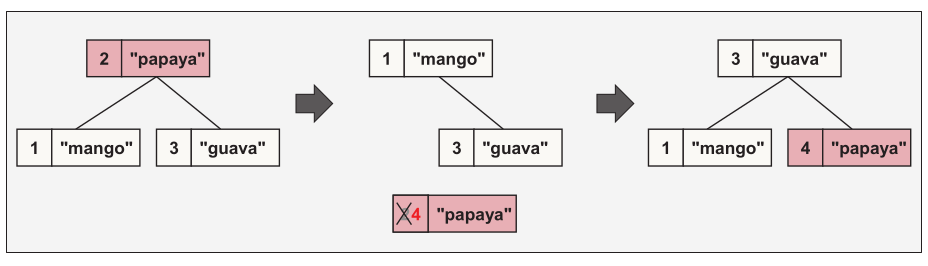
\includegraphics[scale=0.67]{../imgs/26.1.png}
    \caption{使用节点句柄修改key}
    \label{f26.1}
\end{figure}

注意在C++17之前如果想修改一个key,必须先删除旧节点然后再插入一个value相同的新节点(key是\\
\texttt{const}的,因为key的值决定了它们在容器中的位置,所以必须保持稳定)。
如果我们使用节点句柄,将不会发生内存分配,并且所有指向元素的指针和引用都保持有效,
然而,当元素还在节点句柄里而不在容器里的时候使用这些指针或者引用会导致未定义的行为。

节点句柄的类型是\emph{container}\texttt{::node\_type}。它提供了下列成员:
\begin{itemize}
    \item 所有(unordered) set类型都有\texttt{value()}成员
    \item 所有(unordered) map类型都有\texttt{key()}和\texttt{mapped()}成员
\end{itemize}

\subsection{在容器之间移动节点句柄}
你也可以使用节点句柄把一个元素从一个容器move(\emph{splice})到另一个容器。
即使容器的类型有如下不同也没有问题:
\begin{itemize}
    \item 一个支持重复而另一个不支持(例如,你可以把一个元素从multimap移动到map)
    \item 比较函数和哈希函数都不同
\end{itemize}
例如,考虑下面的程序:
\inputcodefile{lib/nodemove.cpp}
我们两次从\texttt{src}中提取元素(一次传递迭代器一次传递key)并把它们插入\texttt{dst}。
因此,程序会有如下输出:
\begin{blacklisting}
    values:
      [1.1:one]  [2.2:two]  [3.3:three]
      [3.3:old data]
    values:
      [3.3:three]
      [1.1:one]  [2.2:two]  [3.3:old data]
\end{blacklisting}
注意当不允许重复时(set、map、unordered set、unordered map),以节点句柄为参数
的\texttt{insert()}成员函数会返回一个有三个成员的结构体类型\emph{container}\texttt{::insert\_return\_type},
三个成员分别是(按照如下顺序):\label{insert节点句柄}
\begin{itemize}
    \item 一个迭代器\textbf{\texttt{position}},当插入成功时(不存在相同key的元素时)指向插入的新元素,
    当插入失败时指向已经存在的元素。
    \item 一个bool值\textbf{\texttt{inserted}}来表示插入是否成功。
    \item 一个\emph{container}\texttt{::node\_type}类型的\textbf{\texttt{node}},当插入失败时作为节点句柄。
\end{itemize}
也就是说,关键信息是第二个成员\texttt{inserted}。通过使用\nameref{ch1},你可以像下面这样使用返回值:
\begin{lstlisting}
    auto [pos, done, node] = dst.insert(src.extract(3.3));
    if (!done) {
        std::cout << "insert() of node handle failed:"
                  << " tried to insert key '" << node.key()
                  << "' with value '" << node.mapped()
                  << "' but key exists with value '" << pos->second << "'\n";
    }
\end{lstlisting}
如果一个元素被提取之后再也没有被重新插入,那么节点句柄的析构函数会释放该元素的内存。
因此,在这段代码中,即使插入失败也不会有内存泄露。

\subsection{合并容器}
以节点句柄API为基础,现在所有的关联和无序容器都提供了成员函数\texttt{merge()},
它可以把一个容器中的所有元素合并到另一个容器中。

再强调一次,即使容器的类型有如下不同也没有问题:
\begin{itemize}
    \item 一个支持重复而另一个不支持(例如,你可以把一个元素从multimap移动到map)
    \item 比较函数和哈希函数都不同
\end{itemize}
如果源容器中的某个元素因为在目标容器里已经有了key相同的元素而无法移动,
那么它会仍然留在源容器中。

例如,下面的程序:
\inputcodefile{lib/nodemerge.cpp}
会有如下输出:
\begin{blacklisting}
    values:
      [1.1:one]  [2.2:two]  [3.3:three]
      [3.3:old data]
    values:
      [3.3:three]
      [1.1:one]  [2.2:two]  [3.3:old data]
\end{blacklisting}
指向被合并元素的指针和引用仍然有效,只不过指向的容器发生了变化。


\section{emplace改进}

\subsection{emplace函数的返回类型}
对于顺序容器\texttt{std::vector<>}、\texttt{std::deque<>}、\texttt{std::list<>}和\texttt{std::forward\_list<>},
还有容器适配器\texttt{std::queue<>}和\texttt{std::stack<>},它们的emplace函数现在
返回新插入的对象的引用(关联容器以前就已经是这样了)。
这允许我们实现类似于如下的代码:
\begin{lstlisting}
    foo(myVector.emplace_back(...));
\end{lstlisting}
来代替:
\begin{lstlisting}
    myVector.emplace_back(...);
    foo(myVector.back());
\end{lstlisting}

\subsection{map的\texttt{try\_emplace()}和\texttt{insert\_or\_assign()}}
这两个成员函数让我们能够稍稍更简单或者更高效的编写处理map和unordered map的代码:
\begin{itemize}
    \item \texttt{try\_emplace()}用移动语义构造一个新的值。
    \item \texttt{insert\_or\_assign()}稍微改进了插入/更新元素的方法。
\end{itemize}

\subsection{\texttt{try\_emplace()}}
考虑下列代码:
\begin{lstlisting}
    std::map<int, std::string> m;
    m[42] = "hello";
    std::string s{"world"};
    m.emplace(42, std::move(s));    // 可能移动,但如果42已经存在时可能不会移动
\end{lstlisting}
这个调用之后\texttt{s}是否仍然保持原本的值是未定义的。
同样,对\texttt{unordered\_map}使用了\texttt{insert()}之后也是这样:
\begin{lstlisting}
    m.insert({42, std::move(s)});   // 可能移动,但如果42已经存在时可能不会移动
\end{lstlisting}
注意根据移动语义的规则这个行为并不是错误。当使用\texttt{std::move(s)}时,
我们只是表明我们对\texttt{s}的值不再感兴趣,\texttt{std::move()}会把对象标记为
可移动的但不会立刻移动走它的值。因此,在这样的调用之后,\texttt{s}\textbf{可能还有也可能没有}
原本的值了。

然而,你可能会惊讶于即使没有成功插入\texttt{s}的值也可能会被移动走(这种情况的发生和实现细节有关)。
有时,程序员可能想或者必须知道对象的值到底有没有被移走,或者想在只有插入成功时才移动走对象的值。
特别的,当使用只能移动的对象例如线程或者独占指针时就是这种情况。

例如,下面的代码是无效的,因为你必须在一个\texttt{std::thread}的析构函数被调用之前
调用它的\texttt{join()}(或者\texttt{detach()})函数:
\begin{lstlisting}
    std::map<int, std::thread> m;
    std::thread t1{...};
    m.insert({42, std::move(t1)});      // 即使没能插入也可能move
\end{lstlisting}
这里,即使\texttt{t1}没有被插入也可能会被move,这会导致core dump,
因为之后\texttt{t1}会在调用内部被销毁并且没有调用\texttt{t1.join()}。
作为代替,你可能必须像下面这样写:
\begin{lstlisting}
    auto pos = m.find(42);
    if (pos == m.end()) {
        m.insert({42, std::move(t1)});  // 如果不存在则插入(并move)
    }
\end{lstlisting}
这样写不仅代码变复杂了,还需要查找新的元素两次。

新的成员函数\texttt{try\_emplace()}保证在没有已存在元素时才会move走传入的值:
\begin{lstlisting}
    m.try_emplace(42, std::move(t1));   // 如果插入失败则不会move
\end{lstlisting}
事实上,它类似于如下写法的缩写:
\begin{lstlisting}
    auto pos = m.find(42);
    if (pos == m.end()) {
        m.emplace(42, std::move(t1));   // 插入
    }
\end{lstlisting}
不过相比之下一个好处是只会查找一次要插入的位置。

就像名字暗示的一样,\texttt{try\_emplace()}允许我们传递任意数量的参数来
在元素不存在时初始化一个新的元素:
\begin{lstlisting}
    std::map<int, std::string> ms;
    ms.try_emplace(42, "hello");    // 尝试插入元素,value为"hello"
    ms.try_emplace(43, 8, 'a');     // 尝试插入元素,value为"aaaaaaaa"
\end{lstlisting}
然而,注意你不能以这种方式初始化一个容器里的元素:
\begin{lstlisting}
    std::map<int, std::vector<std::string>> vals;
    std::string h{"hello"};
    std::string w{"world"};
    vals.try_emplace(42, std::vector<std::string>{h, w});   // OK
    vals.try_emplace(42, h, w);                             // ERROR
\end{lstlisting}
可以传递一个额外的迭代器作为第一个参数,它被用作查找新元素应该放置的位置时的提示。

\subsection{\texttt{insert\_or\_assign()}}
另外,新的成员函数\texttt{insert\_or\_assign()}保证把值移动到一个新的元素或者已存在的元素中:
\begin{lstlisting}
    m.insert_or_assgin(42, std::move(t1));  // 总是会move
\end{lstlisting}
它的行为类似于如下代码的缩写:
\begin{lstlisting}
    auto pos = m.find(42);
    if (pos == m.end()) {
        m.insert({42, std::move(t1)});  // 插入
    }
    else {
        pos->second = std::move(t1);    // 更新
    }
\end{lstlisting}
类似于
\begin{lstlisting}
    m[42] = std::move(t1);              // key不存在时首先默认初始化value,再覆盖value
\end{lstlisting}
不过相比之下的好处是新元素的位置只会查找一次,并且新元素并不是首先用默认构造函数构造然后再覆写。

因此,这个成员函数可以在默认构造函数不能调用的情况下允许我们插入或者更新一个元素。

注意\texttt{insert\_or\_assign()}把key和value作为分离的参数,而\texttt{insert()}
把它们作为一个整体参数。
另外,可以传递一个额外的迭代器作为第一个参数,它被用作查找新元素应该放置的位置时的提示。


\section{对不完全类型的容器支持}
自从C++17起,\texttt{std::vector}、\texttt{std::list}、\texttt{std::forward\_list}被要求支持
不完全类型。

这个特性的主要动机在Matt Austern的一篇标题
为\emph{The Standard Librarian: Containers of Incomplete Types}
的文章中进行了解释:
\footnote{见\url{See http://web.archive.org/web/20190305220304/http://www.drdobbs.com/184403814}。}
你现在可以定义一个类型,内部递归的包含一个自身类型的容器。例如:
\begin{lstlisting}
    struct Node
    {
        std::string value;
        std::vector<Node> children; // 自从C++17起OK(这里Node是一个不完全的类型)
    };
\end{lstlisting}
这也适用于带有private成员和public API的类。
这里有一个完整的例子:
\inputcodefile{lib/incomplete.hpp}
你可以像下面这样使用这个类:
\inputcodefile{lib/incomplete.cpp}
程序会有如下输出:
\begin{blacklisting}
    top
      elem1
        elem1.1
      elem2
\end{blacklisting}


\section{string改进}
对于string(类型为\texttt{basic\_string<>)},C++17提供了以下一些改进:
\begin{itemize}
    \item 对于非常量string,你现在也可以调用\texttt{data()}把底层的字符序列当作原生C字符串来访问:
    \begin{lstlisting}
    std::string mystring{"Hello world"};
    auto cstr = mystring.data();
    cstr[6] = 'W';                      // 自从C++17起OK
    \end{lstlisting}
    注意在C++17之前,\texttt{cstr}的类型将是\texttt{const char*},而现在它的类型是\texttt{char*}。
    在C++17之前,把\texttt{data()}的返回值赋值给\texttt{char*}将不能通过编译:
    \begin{lstlisting}
    std::string mystring{"Hello world"};
    char* cstr = mystring.data();   // 自从C++17起OK
    \end{lstlisting}
    和以前一样,只要\texttt{std::string}还存在并且没有重新分配内存,
    对\texttt{data()}的返回值的访问就是有效的。修改\texttt{data()}返回值的末尾的空终止符仍然是未定义行为。
    \item 还提供了一个到\texttt{std::string\_view}的隐式转换,然而,这可能会导致一些bug或者歧义。
    见\hyperref[ch19]{关于字符串视图的章节}获取详情。
    \item 字符串现在也支持多态类型资源,这意味着你可以声明:
    \begin{lstlisting}
    std::pmr::string s1;
    std::pmr::wstring s1;
    std::pmr::u16string s1;
    std::pmr::u32string s1;
    \end{lstlisting}
    见\hyperref[ch29]{PMR章节}获取详情。
\end{itemize}


\section{后记}
Alan Talbot在\url{https://wg21.link/lwg839}中要求拼接操作、
Alisdair Meredith在\url{https://wg21.link/lwg1041}中要求节点元素要有更多操作支持,
这两个提案都是作为标准库的issue提出,间接的首次提出了节点句柄的概念。

最终被接受的是Alan Talbot、Jonathan Wakely、Howard Hinnant、James Dennett
发表于\url{https://wg21.link/p0083r3}的提案。
Howard E. Hinnant在\url{https://wg21.link/p0508r0}中稍微修改使API更加明晰,并成为了最终版本的API。

emplace成员函数的新返回值类型由Alan Talbot在\url{https://wg21.link/p0084r0}中首次提出。
最终被接受的是Alan Talbot发表于\url{https://wg21.link/p0084r2}的提案。

(unordered) map的\texttt{insert\_or\_assign()}和\texttt{try\_emplace()}操作由
Thomas Köppe在\url{https://wg21.link/n3873}中首次提出。
最终被接受的是Thomas Köppe发表于\url{https://wg21.link/n4279}的提案。

对不完全类型的容器支持由Matt Austern在\url{http://drdobbs.com/184403814}中首次讨论,
由Zhihao Yuan在\url{https://wg21.link/n3890}中首次提出。
最终被接受的是Zhihao Yuan发表于\url{https://wg21.link/n4510}的提案。

string的\texttt{data()}支持由Michael Bradshaw在\url{https://wg21.link/lwg2391}
中作为标准库的issue首次提出。最终被接受的是David Sankel发表于\url{https://wg21.link/p0272r1}的提案。

    \chapter{多线程和并发}\label{ch27}
C++17还引入了一些多线程和并发领域的扩展和改进。


\section{补充的互斥量和锁}

\subsection{\texttt{std::scoped\_lock}}\label{ch27.1.1}
C++11引入了一个简单的\texttt{std::lock\_guard}来实现简单的RAII风格的
互斥量上锁:
\begin{itemize}
    \item 构造函数上锁
    \item 析构函数解锁(也可能因异常而调用析构函数解锁)
\end{itemize}
不幸的是,没有标准化的可变参数模板可以用来在一条语句中同时锁住多个互斥量。

\texttt{std::scoped\_lock<>}解决了这个问题。它允许我们同时锁住一个或多个互斥量。
互斥量的类型也可以不同。

例如:
\begin{lstlisting}
    #include <mutex>
    ...
    std::vector<std::string> allIssues;
    std::mutex allIssuesMx;
    std::vector<std::string> openIssues;
    std::timed_mutex openIssuesMx;

    // 同时锁住两个issue列表:
    {
        std::scoped_lock lg(allIssuesMx, openIssuesMx);
        ... // 操作allIssues和openIssues
    }
\end{lstlisting}
注意根据\nameref{ch9},声明\texttt{lg}时你不需要指明互斥量的类型。

这个示例等价于下面的C++11代码:
\begin{lstlisting}
    // 锁住两个issue列表:
    {
        std::lock(allIssuesMx, openIssuesMx);   // 以避免死锁的方式上锁
        std::lock_guard<std::mutex> lg1(allIssuesMx, std::adopt_lock);
        std::lock_guard<std::mutex> lg2(openIssuesMx, std::adopt_lock);
        ... // 操作allIssues和openIssues
    }
\end{lstlisting}
因此,当传入的互斥量超过一个时,\texttt{scoped\_lock}的构造函数会使用可变参数的
快捷函数\texttt{lock(...)},这个函数会保证不会导致死锁
(标准中提到:\emph{“必须使用一个避免死锁的算法,例如try-and-back-off算法,但具体
使用哪种算法并没有明确指定,这是为了避免过度约束实现”})。

如果只向\texttt{scoped\_lock}的构造函数传递了一个互斥量,那么它只简单的锁住互斥量。
因此,如果用单个参数构造\texttt{scoped\_lock},它的行为类似于\texttt{lock\_guard}。
它还定义了成员\texttt{mutex\_type},而多个互斥量构造的对象没有这个成员。
\footnote{典型的实现是提供一个单互斥量参数的偏特化版本。}
因此,你可以把所有的\texttt{lock\_guard}都替换为\texttt{scoped\_lock}。

如果没有传递互斥量,那么将不会有任何效果。

注意你也可以传递已经被锁住的互斥量:
\begin{lstlisting}
    // 锁住两个issue列表:
    {
        std::lock(allIssuesMx, openIssuesMx);   // 注意:使用了避免死锁的算法
        std::scoped_lock lg{std::adopt_lock, allIssuesMx, openIssuesMx};
        ... // 操作allIssues和openIssues
    }
\end{lstlisting}
然而,注意现在传递已经被锁住的互斥量时要在前边加上\texttt{adopt\_lock}参数。
\footnote{在最初的C++17标准中\texttt{adopt\_lock}参数是在最后,之后在
\url{https://wg21.link/p0739r0}中修正。}

\subsection{\texttt{std::shared\_mutex}}
C++14添加了一个\texttt{std::shared\_timed\_mutex}来支持读/写锁,
它支持多个线程同时读一个值,偶尔会有一个线程更改值。
然而,在某些平台上不支持超时的锁可以被实现的更有效率。
因此,现在引入了类型\texttt{std::shared\_mutex}
(就像C++11引入的\texttt{std::mutex}和\texttt{std::timed\_mutex}的关系一样)。

\texttt{std::shared\_mutex}定义在头文件\texttt{shared\_mutex}中,支持以下操作:
\begin{itemize}
    \item 对于独占锁:\texttt{lock}、\texttt{try\_lock()}、\texttt{unlock()}
    \item 对于共享的读访问:\texttt{lock\_shared()}、\texttt{try\_lock\_shared()}、\texttt{unlock\_shared()}
    \item \texttt{native\_handle()}
\end{itemize}
也就是说,和类型\texttt{std::shared\_timed\_mutex}不同的地方在于,
\texttt{std::shared\_mutex}不保证支持\texttt{try\_\\
lock\_for()}、\texttt{try\_lock\_until()}、\texttt{try\_lock\_shared\_for()}、\texttt{try\_lock\_shared\_until}等操作。

注意\texttt{std::shared\_timed\_mutex}是唯一一个不提供\texttt{native\_handle()} API的互斥量类型。

\subsubsection{使用\texttt{shared\_mutex}}
我们可以像这样使用\texttt{shared\_mutex}:假设你有一个共享的vector,它被多个线程读取,
但偶尔会被修改:
\begin{lstlisting}
    #include <shared_mutex>
    #include <mutex>
    ...
    std::vector<double> v;      // 共享的资源
    std::shared_mutex vMutex;   // 控制对v的访问(在C++14中要使用shared_timed_mutex)
\end{lstlisting}
为了获取共享的读权限(多个读者不会互相阻塞),你可以使用\texttt{std::shared\_lock},
它是为共享读权限设计的lock guard(C++14引入)。例如:
\begin{lstlisting}
    if (std::shared_lock sl(vMutex); v.size() > 0) {
        ... // vector v的(共享)读权限
    }
\end{lstlisting}
对于独占的写操作你应该使用独占的lock guard。可以使用简单的\texttt{lock\_guard},
或者\texttt{scoped\_lock}(\hyperref[ch27.1.1]{刚刚介绍的})、或者复杂的\texttt{unique\_lock}。例如:
\begin{lstlisting}
    {
        std::scoped_lock sl(vMutex);
        ... // vector v的独占的写权限
    }
\end{lstlisting}


\section{原子类型的\texttt{is\_always\_lock\_free}}
你现在可以使用一个C++库的特性来检查一个特定的原子类型是否总是可以在无锁的情况下使用。例如:
\begin{lstlisting}
    if constexpr(std::atomic<int>::is_always_lock_free) {
        ...
    }
    else {
        ...
    }
\end{lstlisting}
如果一个原子类型的\texttt{is\_always\_lock\_free}返回\texttt{true},
那么该类型的对象的\texttt{is\_lock\_free()}成员一定会返回\texttt{true}:
\begin{lstlisting}
    if constexpr(atomic<T>::is_always_lock_free) {
        assert(atomic<T>{}.is_lock_free()); // 绝不会失败
    }
\end{lstlisting}
在C++17之前只能使用相应的宏的值来判断。例如,
当且仅当\texttt{ATOMIC\_INT\_LOCK\_FREE}返回\texttt{2}时(这个值代表“总是”)
\texttt{std::atomic<int>::is\_always\_lock\_free}为\texttt{true},
\begin{lstlisting}
    if constexpr(std::atomic<int>::is_always_lock_free) {
        // ATOMIC_INT_LOCK_FREE == 2
        ...
    }
    else {
        // ATOMIC_INT_LOCK_FREE == 0 || ATOMIC_INT_LOCK_FREE == 1
        ...
    }
\end{lstlisting}
用静态成员替换宏是为了确保类型更加安全和在复杂的泛型代码中使用这些检查(例如,使用SFINAE时)。

记住\texttt{std::atomic<>}也可以用于平凡的可拷贝类型。因此,
你可以检查如果把你自定义的结构体用作原子类型时是否需要锁。例如:
\begin{lstlisting}
    template<auto SZ>
    struct Data {
        bool set;
        int values[SZ];
        double average;
    };

    if constexpr(std::atomic<Data<4>>::is_always_lock_free) {
        ...
    }
    else {
        ...
    }
\end{lstlisting}


\section{cache行大小}
有时有的程序很需要处理cache行大小的能力:
\begin{itemize}
    \item 一方面,不同线程访问的不同对象不属于同一个cache行是很重要的。
    否则,不同线程并发访问对象时cache行缓存的内存可能需要同步。
    \footnote{在C++中多个线程并发访问不同的对象通常是安全的,但是必要的同步可能会降低程序的性能。}
    \item 另一方面,你可能会想把多个对象放在同一个cache行中,这样访问了第一个对象之后,
    访问接下来的对象时就可以直接在cache中访问它们,不用再把它们调入cache。
\end{itemize}
为了实现这一点,C++标准库在头文件\texttt{<new>}引入了两个\nameref{ch3}:
\begin{lstlisting}
    namespace std {
        inline constexpr size_t hardware_destructive_interference_size;
        inline constexpr size_t hardware_constructive_interference_size;
    }
\end{lstlisting}
这些对象有下列实现定义的值:
\begin{itemize}
    \item \texttt{hardware\_destructive\_interference\_size}是推荐的
    可能被不同线程并发访问的两个对象之间的最小偏移量,再小的话就可能有性能损失,
    因为共用的L1缓存会被影响。
    \item \texttt{hardware\_constructive\_interference\_size}是推荐的
    两个想被放在同一个L1缓存行的对象合起来的最大大小。
\end{itemize}
这两个值都只是建议因为实际的值依赖于具体的架构。
这两个值只是编译器在生成支持的不同平台的代码时可以提供的最佳的值。
因此,如果你知道更好更准确的值,那就使用你知道的值。
不过使用这两个值要比使用假设的不同平台的固定大小更好。

这两个值都至少是\texttt{alignof(std::max\_align\_t)}。并且这两个值通常是相等的。
然而,从语义上讲,它们代表了不同的目的,所以你应该像下面这样根据情况使用它们:
\begin{itemize}
    \item 如果你想在\emph{不同的线程里}访问两个不同的(原子)对象:
    \begin{lstlisting}
    struct Data {
        alignas(std::hardware_destructive_interference_size) int valueForThreadA;
        alignas(std::hardware_destructive_interference_size) int valueForThreadB;
    };
    \end{lstlisting}
    \item 如果你想在\emph{同一个线程里}访问两个不同的(原子)对象:
    \begin{lstlisting}
    struct Data {
        int valueForThraedA;
        int otherValueForTheThreadA;
    };

    // 再检查一次我们能通过共享的cache行获得最佳性能
    static_assert(sizeof(Data) <= std::hardware_constructive_interference_size);

    // 确保对象被恰当的对齐:
    alignas(sizeof(Data)) Data myDataForAThread;
    \end{lstlisting}
\end{itemize}

\section{后记}
\texttt{scoped\_lock}最初由Mike Spertus在\url{https://wg21.link/n4470}中提议
把\texttt{lock\_guard}改为可变参数,最后作为\url{https://wg21.link/p0156r0}提案被接受了。
然而,因为这会导致ABI的不兼容,所以Mike Spertus又在\url{https://wg21.link/p0156r2}中引入了
新的名字\texttt{scoped\_lock},并且最终被接受。
Mike Spertus、Walter E. Brown和Stephan T. Lavavej之后在\url{https://wg21.link/p0739r0}
中作为C++17的缺陷修改了构造函数的参数顺序。

\texttt{shared\_mutex}最早和所有其他C++11引入的互斥量一起由Howard Hinnant在
\url{https://wg21.link/n2406}中提出。
然而,让C++标准委员会相信所有的互斥量都很有用消耗了很长时间。
因此它直到C++17才被接受,最终被接受的是Gor Nishanov发表于\url{https://wg21.link/n4508}的提案。

\texttt{std::atomic<>}的静态成员\texttt{std::is\_always\_lock\_free}
由Olivier Giroux、JF Bastien和Jeff Snyder在\\
\url{https://wg21.link/n4509}中首次提出。
最终被接受的是Olivier Giroux、JF Bastien和Jeff Snyder发表于\url{https://wg21.link/p0152r1}的提案。

硬件的干扰因素(cache行)的大小由JF Bastien和Olivier Giroux在\url{https://wg21.link/n4523}中
首次提出。最终被接受的是JF Bastien和Olivier Giroux发表于\url{https://wg21.link/p0154r1}的提案。

    \chapter{标准库的其他微小特性和修改}\label{ch28}
C++标准库还有一些微小的扩展和变化,将在这一章中描述。


\section{\texttt{std::uncaught\_exceptions()}}\label{ch28.1}
C++的一个关键模式是\emph{RAII: Resource Acquisition Is Initialization}。
这是一种安全地处理那些你必须要释放或清理的资源的方式。
在构造一个对象时把需要的资源的所有权传递给它,当离开作用域时它的析构函数就会自动释放资源。
这样做的好处是即使因为异常而离开当前作用域时也能保证释放资源。

然而,有时资源的“释放操作”依赖于我们到底是正常执行离开了作用域还是因为异常而意外离开了作用域。
一个例子是事务性的资源,如果我们正常执行离开作用域我们可能想进行\emph{提交}操作,
而当因为异常离开作用域时想进行\emph{回滚}操作。

为了达到这个目的,C++11引入了\texttt{std::uncaught\_exception()},其用法如下所示:
\begin{lstlisting}
    class Request {
    public:
        ...
        ~Request() {
            if (std::uncaught_exception()) {
                rollback();
            }
            else {
                commit();
            }
        }
    };
\end{lstlisting}
因此,当\texttt{Request}对象离开作用域时会根据是否有异常抛出来
决定到底是调用\texttt{commit()}还是\texttt{rollback()}。
\begin{lstlisting}
    {
        Request r1{...};    // 没有异常时析构函数会调用commit()
        ...
        if (...) {
            throw ...;      // 让析构函数调用rollback()
        }
        ...
    }   // 正常时调用commit(),异常时调用rollback()
\end{lstlisting}
然而,在如下使用场景中这个API不能正常工作:\emph{当我们正在处理异常时}
如果创建了新的\texttt{Request}对象,那么即使在使用它的期间没有异常抛出
它的析构函数也总是会调用\texttt{rollback()}:
\begin{lstlisting}
    try {
        ...
    }
    catch (...) {
        Request r2{...};
        ...
    }   // 即使在catch语句块中没有出现新的异常也会调用rollback()
\end{lstlisting}
新的标准库函数\texttt{uncaught\_exceptions()}(注意名字最后多出来的\texttt{s})
解决了这个问题。它返回有多少个(嵌套的)还未处理的异常,而不是我们是否正在处理一个异常。
这允许我们查明是否有额外的异常抛出(即使在处理异常时)。

有了这个,我们可以简单的对\texttt{Request}的定义做如下修改:
\begin{lstlisting}
    class Request {
    private:
        int initialUncaught{std::uncaught_exceptions()};
    public:
        ...
        ~Request() {
            if (std::uncaught_exceptions() > initialUncaught) {
                rollback();
            }
            else {
                commit();
            }
        }
    };
\end{lstlisting}
现在下面两个示例场景都能正常工作:
\begin{lstlisting}
    try {
        Request r1{...};    // 没有异常时析构函数会调用commit()
        ...
        if (...) {
            throw ...;      // 让析构函数调用rollback()
        }
        ...
    }   // 正常时调用commit(),异常时调用rollback()
    catch (...) {
        Request r2{...};
        ...
    }   // 如果没有额外的异常发生就调用commit()
\end{lstlisting}
这里,\texttt{r2}的构造函数把\texttt{initialUncaught}初始化为\texttt{1},
因为我们已经在\texttt{catch}语句块中处理了一个异常。
然而,当\texttt{r2}的析构函数调用时没有新的异常抛出,所以\texttt{initialUncaught}仍然
是\texttt{1},因此会调用\texttt{commit()}。如果在\texttt{catch}子句中又抛出了第二个未
捕获的异常那么\texttt{std::uncaught\_exceptions()}将会返回\texttt{2},因此\texttt{r2}的
析构函数会调用\texttt{rollback()}。

见\emph{lib/uncaught.cpp}获取完整的示例。
\footnote{译者注:lib/uncaught.cpp见\url{https://www.cppstd17.com/code/lib/uncaught.cpp.html}。}

旧的API \texttt{std::uncaught\_exception()}(没有末尾的\texttt{s})自从C++17起被废弃,不应该再被使用。


\section{共享指针改进}
C++17中也添加了一些共享指针的改进。

另外,注意成员函数\hyperref[ch35.2.7]{\texttt{unique()}已经被废弃了}。

\subsection{对原生C数组的共享指针的特殊处理}\label{ch28.2.1}
自从C++17起,你可以显式的声明数组的共享指针来确保deleter会调用\texttt{delete[]}
(自从C++11起独占指针就已经可以做到):你现在可以简单地调用:
\begin{lstlisting}
    std::shared_ptr<std::string[]> p{new std::string[10]};
\end{lstlisting}
来代替:
\begin{lstlisting}
    std::shared_ptr<std::string> p{new std::string[10], std::default_delete<std::string[]>()};
\end{lstlisting}
或者:
\begin{lstlisting}
    std::shared_ptr<std::string> p{new std::string[10], [](std::string* p) {
                                                            delete[] p;
                                                        }};
\end{lstlisting}
当实例化的是数组时,API也会有一些变化:不再是使用\texttt{operator*},而是使
用\texttt{operator[]}(就像独占指针一样):
\begin{lstlisting}
    std::shared_ptr<std::string> ps{new std::string};
    *ps = "hello";      // OK
    ps[0] = "hello";    // ERROR

    std::shared_ptr<std::string[]> parr{new std::string[10]};
    *parr = "hello";    // ERROR(未定义行为)
    parr[0] = "hello";  // OK
\end{lstlisting}
注意分配的是原生数组时是否支持\texttt{operator*}和分配的不是数组时是否支持\texttt{operator[]}
还没有明确的定义。然而,通常情况下调用这些未定义的运算符不能编译。

\subsection{共享指针的\texttt{reinterpret\_pointer\_cast}}
除了\texttt{static\_pointer\_cast}、\texttt{dynamic\_pointer\_cast}、\texttt{const\_pointer\_cast}之外,
你现在还可以调用\texttt{reinterpret\_pointer\_cast}重新解释一个共享指针指向的若干位的类型。

\subsection{共享指针的\texttt{weak\_type}}
为了支持在泛型代码中使用弱指针,共享指针类现在提供了一个新的成员\texttt{weak\_type}。例如:
\begin{lstlisting}
    template<typename T>
    void observe(T sp)
    {
        // 用传入的共享指针初始化弱指针
        typename T::weak_type wp{sp};
        ...
    }
\end{lstlisting}

\subsection{共享指针的\texttt{weak\_from\_this}}
有时你需要另一个智能指针来指向一个已经存在的对象,并且不想访问已经指向该对象的其他共享指针。
为了解决这个问题,C++11引入了基类\texttt{enable\_shared\_from\_this},
它提供了成员函数\texttt{shared\_from\_this}:
\begin{lstlisting}
    #include <memory>

    class Person : public std::enable_shared_from_this<Person>
    {
        ...
    };

    Person* pp = new Person{...};
    std::shared_ptr<Person> sp1{pp};    // sp1获得了所有权
    std::shared_ptr<Person> sp2{pp};    // 运行时错误:sp2不能再获取所有权
    std::shared_ptr<Person> sp3{pp->shared_from_this()};    // OK:sp1和sp3共享所有权
\end{lstlisting}
如果该对象的一个成员函数需要返回一个自身的共享指针时就会用到这个特性:
\begin{lstlisting}
    class Person : public std::enable_shared_from_this<Person>
    {
        ...
        std::shared_ptr<Person> sharedPtrTo() {
            return shared_from_this();
        }
    }
\end{lstlisting}
自从C++17开始,有一个额外的辅助函数可以返回一个指向对象的弱指针:
\begin{lstlisting}
    Person* pp = new Person{...};
    std::shared_ptr<Person> sp{pp};                 // sp获得了所有权
    ...
    std::weak_ptr<Person> wp{pp->weak_from_this()}; // wp分享了sp拥有的所有权
\end{lstlisting}
在C++17之前,你可以用如下代码实现同样的功能:
\begin{lstlisting}
    weak_ptr<Person> wp{pp->shared_from_this()}
\end{lstlisting}
但是\texttt{weak\_from\_this()}可以在修改更少的引用计数的情况下实现相同的效果。
另外,还要说明一种特殊的边界情况:如果一个原生指针被传递给两个不同的共享指针
(如果它们中只有一个最终释放了资源那么这是有效的),那么\texttt{shared\_from\_this()}
和\texttt{weak\_from\_this()}会分享第一个共享指针的所有权。
这意味着下面的代码是可行的:
\begin{lstlisting}
    struct Person : public std::enable_shared_from_this<Person>
    {
        ...
    };

    Person* p = new Person;
    std::shared_ptr<Person> sp1(p);         // 创建第一个共享指针

    {
        std::shared_ptr<Person> sp2(p,      // 创建第二个不会释放资源的共享指针
                                    [] (void*) {
                                    });
        auto sp3{p->shared_from_this()};    // sp3分享sp1的所有权
    }

    auto sp4{p->shared_from_this()};        // sp4分享sp1的所有权
\end{lstlisting}
在这个情况得到说明之前,一些实现让\texttt{sp3}和\texttt{sp4}分享\emph{最后}创建的
共享指针的所有权,这会导致当初始化时\texttt{sp4}抛出\texttt{std::bad\_weak\_ptr}异常。


\section{数学扩展}
C++17还引入了下面的数学函数。

\subsection{最大公约数和最小公倍数}
在头文件\texttt{<numeric>}中:
\begin{itemize}
    \item \texttt{gcd(x, y)}返回\texttt{x}和\texttt{y}的\emph{最大公约数}。
    \item \texttt{lcm(x, y)}返回\texttt{x}和\texttt{y}的\emph{最小公倍数}。
\end{itemize}
参数的类型都是除了\texttt{bool}以外的整数类型。两个参数的类型可以不同,
此时返回值的类型将是两个参数的公共类型。

例如:
\begin{lstlisting}
    #include <numeric>

    int i{42};
    long l{30};

    auto x{std::gcd(i, l)};     // x是long 6
    auto y{std::lcm(i, l)};     // y是long 210
\end{lstlisting}

\subsection{\texttt{std::hypot()}的三参数重载}
在头文件中\texttt{<cmath>}中:
\begin{itemize}
    \item \texttt{hypot(x, y, z)}返回三个参数的平方之和的平方根。
\end{itemize}
就像\texttt{<cmath>}中其他的函数一样,这个函数有支持所有浮点数类型的重载版本。

这些重载在\texttt{math.h}或者命名空间\texttt{std}之外是没有的。

例如:
\begin{lstlisting}
    #include <cmath>

    // 计算3D坐标下两个点的距离:
    auto dist = std::hypot(p2.x - p1.x, p2.y - p1.y, p2.z - p1.z);
\end{lstlisting}
在C++17之前,你必须像下面这样调用:
\begin{lstlisting}
    auto dist = std::hypot(p2.x - p1.x, std::hypot(p2.y - p1.y, p2.z - p1.z));
\end{lstlisting}

\subsection{数学的特殊函数}
表\hyperref[t28.1]{数学的特殊函数}中的一部分已经在国际标准IS 29124:2010中标准化,
现在被要求无条件的加入C++标准中的头文件\texttt{<cmath>}中。
\begin{table}[htb]
    \centering
    \begin{tabular}{l|l}
        \hline
        \textbf{名称}              &            \textbf{含义} \\
        \hline
        \texttt{assoc\_laguerre()} & 关联Laguerre多项式       \\
        \texttt{assoc\_legendre()} & 关联Legendre函数        \\
        \texttt{beta()}            & beta函数              \\
        \texttt{comp\_ellint\_1()} & 第一类完整椭圆积分           \\
        \texttt{comp\_ellint\_2()} & 第二类完整椭圆积分           \\
        \texttt{comp\_ellint\_3()} & 第三类完整椭圆积分           \\
        \texttt{cyl\_bessel\_i()}  & 规则圆柱贝塞尔函数变体         \\
        \texttt{cyl\_bessel\_j()}  & 第一类圆柱贝塞尔函数          \\
        \texttt{cyl\_bessel\_k()}  & 不规则圆柱贝塞尔函数变体        \\
        \texttt{cyl\_neumann()}    & 圆柱诺依曼函数(第二类圆柱贝塞尔函数) \\
        \texttt{ellint\_1()}       & 第一类不完整椭圆积分          \\
        \texttt{ellint\_2()}       & 第二类不完整椭圆积分          \\
        \texttt{ellint\_3()}       & 第三类不完整椭圆积分          \\
        \texttt{expint()}          & 指数积分                \\
        \texttt{hermite()}         & Hermite多项式          \\
        \texttt{laguerre()}        & Laguerre多项式         \\
        \texttt{legendre()}        & Legendre多项式         \\
        \texttt{riemann\_zeta()}   & 黎曼zeta函数            \\
        \texttt{sph\_bessel()}     & 第一类球形贝塞尔函数          \\
        \texttt{sph\_legendre()}   & 关联球形Legendre函数      \\
        \texttt{sph\_neumann()}    & 球形诺依曼函数(第二类球形贝塞尔函数) \\
        \hline
    \end{tabular}
    \caption{数学的特殊函数}
    \label{t28.1}
\end{table}

这些函数的参数都是浮点数,返回值是\texttt{double}。
所有这些函数还有
\begin{itemize}
    \item 后缀\texttt{f}代表参数和返回值的类型是\texttt{float}
    \item 后缀\texttt{l}代表参数和返回值的类型是\texttt{long double}
\end{itemize}
例如:
\begin{lstlisting}
    // 指数积分:
    double      expint(double x);
    float       expintf(float x);
    long double expintl(long double x);

    // Laguerre多项式:
    double      laguerre(unsigned n, double x);
    float       laguerref(unsigned n, float x);
    long double laguerrel(unsigned n, long double x);
\end{lstlisting}

\section{\texttt{chrono}扩展}
C++17还向标准库中的时间库部分添加了一些扩展来增强库的易用性和一致性。

对于时间段和时间点,还添加了新的舍入函数:
\begin{itemize}
    \item \texttt{round()}:舍入到最近的整数值
    \item \texttt{floor()}:向负无穷舍入到最近的整数值
    \item \texttt{ceil()}:向正无穷舍入到最近的整数值
\end{itemize}
这些舍入方法和\texttt{duration\_cast<>}和\texttt{time\_point\_cast<>}
(在C++17之前就已经存在)不同,新的舍入函数不是简单的向0截断。

另外,时间段类型还添加了缺失的\texttt{abs()}函数。

下面的程序演示了时间段类型的行为:
\inputcodefile{lib/chronoext.cpp}
它会有如下输出:
\begin{blacklisting}
    3330ms
      abs():   3330ms
      cast:    3000ms
      floor(): 3000ms
      ceil():  4000ms
      roumd(): 3000ms
    3770ms
      abs():   3770ms
      cast:    3000ms
      floor(): 3000ms
      ceil():  4000ms
      round(): 4000ms
    -3770ms
      abs():   3770ms
      cast:    -3000ms
      floor(): -4000ms
      ceil():  -3000ms
      round(): -4000ms
\end{blacklisting}

\section{\texttt{constexpr}扩展和修正}\label{ch28.5}
就像从C++11开始的每个新版本一样,标准中又在很多地方添加/修正了对\texttt{constexpr}的支持。

最重要的修正有:
\begin{itemize}
    \item 对于\texttt{std::array},下面的函数现在是\texttt{constexpr}:
    \begin{itemize}
        \item \texttt{begin()、end()、cbegin()、cend()、rbegin()、rend()、crbegin()、crend()}
        \item 非常量数组的\texttt{operator[]、at()、front()、back()}
        \item \texttt{data()}
    \end{itemize}
    \item 范围访问的泛型独立函数(\texttt{std::begin()、std::end()、std::rbegin()、std::rend()})
    和辅助函数(\texttt{std::advance()、std::distance()、std:prev()、std::next()})现在也是\texttt{constexpr}。
    \item 类\texttt{std::reverse\_iterator}和\texttt{std::move\_iterator}的所有操作现在都是\texttt{constexpr}。
    \item C++标准库里整个时间库部分(\texttt{time\_point}、\texttt{duration}、时钟、\texttt{ratio}),
    现在除了时钟的成员函数\texttt{now()}、\texttt{to\_time\_t()}、\texttt{from\_time\_t()}之外
    所有操作和变量都是\texttt{constexpr}。
    \item 所有的\texttt{std::char\_traits}特化的成员函数是\texttt{constexpr}。特别的,
    这允许我们\hyperref[编译期字符串视图]{在编译期初始化字符串视图}。
\end{itemize}
例如,你现在可以写:
\begin{lstlisting}
    constexpr std::array arr{0, 8, 15, 42};
    constexpr auto val = arr[2];    // OK
    static_assert(val == 15);       // OK,不会断言失败
\end{lstlisting}
注意对于迭代器,我们需要使用全局的或者\texttt{static}的对象,因为我们不能在编译期
获取栈上的对象的地址:
\begin{lstlisting}
    constexpr static std::array arr{0, 8, 15, 42};
    constexpr auto pos = std::next(arr.begin());    // OK
    static_assert(*pos == 15);                      // OK,不会断言失败
\end{lstlisting}

\section{\texttt{noexcept}扩展和修正}
就像从C++11开始的每个新版本一样,标准中又在很多地方添加/修正了对\texttt{noexcept}的支持。

最重要的修正有:
\begin{itemize}
    \item 对于\texttt{std::vector<>}和\texttt{std::string}(\texttt{std::basic\_string<>}),
    C++17保证下列操作不会抛出异常
    \begin{itemize}
        \item 默认构造函数(前提是提供的分配器的默认构造函数不会抛出异常)
        \item 移动构造函数
        \item 以分配器为参数的构造函数
    \end{itemize}
    \item 对于所有的容器(包括\texttt{std::string/std::basic\_string<>}),C++17保证下列操作不会抛出异常
    \begin{itemize}
        \item 移动赋值运算符(前提是提供的分配器可以互换)
        \item \texttt{swap()}函数(前提是提供的分配器可以互换)
    \end{itemize}
\end{itemize}

\subsubsection{对vector重新分配的影响}
注意\texttt{noexcept}的修正中有一项非常特殊也非常重要:
只有vector和string现在保证不会在移动构造函数中抛出异常。
其他的容器仍然有可能抛出异常。

这一点当在一个vector中使用这几种类型时会产生重要的影响,
如果元素的移动构造函数保证不抛出异常,
那么vector在重新分配时可以简单的使用移动构造函数来移动元素。

换句话说:
\begin{itemize}
    \item 重新分配一个string/vector的vector现在保证会很快速。
    \item 重新分配一个其他容器类型的vector仍然可能很慢。
\end{itemize}
这已经成为了另一个除非必要否则使用vector作为默认容器的原因。

\section{后记}
\texttt{std::uncaught\_exceptions()}的动机由Herb Sutter在\url{https://wg21.link/n3614}中
首次提出。最终被接受的是Herb Sutter发表于\url{https://wg21.link/n4259}的提案。

数组类型的共享指针扩展和添加\texttt{reinterpret\_pointer\_cast}转换由Peter Dimov在
\url{https://wg21.link/n3640}中首次提出。最终被接受的是Jonathan Wakely发表
于\url{https://wg21.link/p0414r2}。

获取共享指针的弱指针类型的访问权限的问题由Arthur O’Dwyer在\url{https://wg21.link/n4537}中首次提出。
最终被接受的是Arthur O’Dwyer发表于\url{https://wg21.link/p0163r0}的提案。

\texttt{weak\_from\_this}由Jonathan Wakely和Peter Dimov在\url{https://wg21.link/p0033r0}中首次提出。
最终被接受的是Jonathan Wakely和Peter Dimov发表于\url{https://wg21.link/p0033r1}的提案。

数学的GCD和LCM函数由Walter E. Brown在\url{https://wg21.link/n3845}中首次提出。
之后它们进入了第一个Library Fundamentals TS。直到C++17,它们按照Walter E. Brown在
\url{https://wg21.link/p0295r0}中的提议被标准库采纳。

三参数的\texttt{std::hypot()}重载由Benson Ma在\url{https://wg21.link/p0030r0}中首次提出。
最终被接受的是Benson Ma发表于\url{https://wg21.link/p0030r1}的提案。

添加特殊数学函数由Walter E. Brown于2003年在\url{https://wg21.link/n1422}中首次提出。
按照国际标准IS 29124:2010强制要求它们进入C++17的提案由Walter E. Brown、Axel Naumann
和Edward Smith-Rowland发表于\url{https://wg21.link/p0226r1}。

时间库扩展由Howard Hinnant在\url{https://wg21.link/p0092r0}中首次提出。
最终被接受的是Howard Hinnant发表于\url{https://wg21.link/p0092r1}的提案。

为时间库添加\texttt{constexpr}由Howard Hinnant在\url{https://wg21.link/p0505r0}中首次提出。
最终被接受的是Howard Hinnant发表于\url{https://wg21.link/p0092R1}的提案。

在其他地方添加\texttt{constexpr}按照Antony Polukhin的
\url{https://wg21.link/p0031r0}和\url{https://wg21.link/p0426r1}提案被标准库采纳。

\texttt{noexcept}的修正由Nicolai Josuttis在\url{https://wg21.link/4002}中首次提出。
这项修改最终被接受的是Nicolai Josuttis发表于\url{https://wg21.link/n4258}的提案。



    \part{专家的工具}\label{part5}
    这一部分介绍了普通应用程序员通常不需要知道的新的语言特性和库。
    它主要包括了为编写基础库和语言特性的程序员准备的用来解决特殊问题语言的特性(例如修改堆内存的管理方式)。

    \chapter{多态内存资源(PMR)}\label{ch29}
自从C++98起,标准库就支持配置类管理自己内部(堆)内存的方式。
因此,标准库中几乎所有会分配内存的类型都有一个分配器参数。
这允许你配置容器、字符串和其他需要栈以外的内存的类型分配内存的方式。

默认分配内存的方式是从堆上分配。然而,出于下列原因你可能会想修改默认的行为:
\begin{itemize}
    \item 你可以使用自己的方式分配内存来减少系统调用。
    \item 你可以确保分配的内存是连续的来受益于CPU缓存。
    \item 你可以把容器和元素放在可以被多个进程访问的共享内存中。
    \item 你甚至可以重定向这些堆内存调用来复用之前在栈上分配的内存。
\end{itemize}
因此,修改默认的行为可能会带来性能和功能上的改进。
\footnote{一开始设置分配器的原因是为了处理不同大小的指针(“near”和“far”指针)。}

然而,直到C++17,(正确地)使用分配器在许多方面都即困难又笨拙
(因为一些语言的缺陷、太过复杂、要考虑向后的兼容性更改)。

C++17现在提供了一种相当容易使用的方法来支持预定义的和用户定义的内存分配方式,
这对标准类型和用户自定义类型都很有用。

因此,这一章将讨论:
\begin{itemize}
    \item 使用标准库提供的\hyperref[ch29.1]{标准内存资源}
    \item 定义\hyperref[ch29.2]{自定义内存资源}
    \item \hyperref[ch29.3]{为自定义类型提供内存资源支持}
\end{itemize}

这一章的完成离不开Pablo Halpern、Arthur O'Dwyer、David Sankel、Jonathan Wakely的帮助。


\section{使用标准内存资源}\label{ch29.1}
这一节介绍了标准内存资源和使用它们的方法。

\subsection{示例}
让我们首先比较一下使用和不使用标准内存资源的内存消耗。

\subsubsection{为容器和字符串分配内存}\label{ch29.1.1.1}
假设你的程序中有一个string的vector,并且你用了很多很长的string来初始化这个vector:
\inputcodefile{pmr/pmr0.cpp}
注意我们使用了\hyperref[ch30.4]{追踪所有\texttt{::new}调用的类}来在下列循环中
追踪内存分配的情况:
\begin{lstlisting}
    std::vector<std::string> coll;
    for (int i = 0; i < 1000; ++i) {
        coll.emplace_back("just a non-SSO string");
    }
\end{lstlisting}
这个过程中会发生很多次内存分配,因为vector使用堆内存来存储元素。
另外,字符串本身也可能在堆上分配空间来存储值
(如果实现使用了短字符串优化,那么通常当字符串超过15个字符时会在堆上分配空间)。

程序的输出可能会像下面这样:
\begin{blacklisting}
    1018 allocations for 134,730 bytes
\end{blacklisting}
这意味着除了每个string要分配一次内存之外,vector内部还分配了18(或者更多)次内存来存储元素。
\footnote{重新分配的次数在不同平台上可能不同,因为重新分配的算法可能会不同。
如果当前的内存容量已经满了,有的实现会将它扩大50\%,然而有的实现会把大小翻倍。}

这样的行为可能会导致很严重的问题,因为内存(重新)分配在一些环境中需要很长时间(例如嵌入式系统),
完全在堆上分配内存可能会导致性能问题。

我们可以事先要求vector预留充足的内存,但一般来说,重新分配内存是不可避免的,除非你事先知道要存储的元素的数量。
如果你不知道具体要处理多少数据,你就必须在避免重新分配和不想浪费太多内存之间权衡。
并且这个例子中至少需要1001次分配(一次分配用来存储vector中的元素,每一个没有使用短字符串优化的string还要分配一次)。

\subsubsection{不为容器分配内存}
我们可以通过使用多态分配器来改进这种情况。
首先,我们可以使用\texttt{std::pmr::vector},并且允许vector在栈上分配自己的内存:
\inputcodefile{pmr/pmr1.cpp}

首先,我们在栈上分配了自己的内存(使用了新类型\nameref{ch18}):
\begin{lstlisting}
    // 在栈上分配一些内存:
    std::array<std::byte, 200000> buf;
\end{lstlisting}
你也可以使用\texttt{char}来代替\texttt{std::byte}。

之后,我们用这些内存初始化了一个\texttt{monotonic\_buffer\_resource},
传递这些内存的地址和大小作为参数:
\begin{lstlisting}
    std::pmr::monotonic_buffer_resource pool{buf.data(), buf.size()};
\end{lstlisting}
最后,我们使用了一个\texttt{std::pmr::vector},它将使用传入的内存资源来分配内存:
\begin{lstlisting}
    std::pmr::vector<std::string> coll{&pool};
\end{lstlisting}
这个声明是下面声明的缩写:
\begin{lstlisting}
    std::vector<std::string, std::pmr::polymorphic_allocator<std::string>> coll{&pool};
\end{lstlisting}
也就是说,我们声明了一个使用\emph{多态分配器}的vector,多态分配器可以在运行时在不同的\emph{内存资源}之间切换。
类\texttt{monotonic\_buffer\_resource}派生自类\texttt{memory\_resource},因此可以
用作多态分配器的内存资源。
最后,通过传递我们的内存资源的地址,可以确保vector的多态分配器使用我们的内存资源。

如果我们测试这个程序中内存分配的次数,输出将是:
\begin{blacklisting}
    1000 allocations for 32000 bytes
\end{blacklisting}
vector的18次内存分配将不会再发生在堆上,而是在我们初始化的\texttt{buf}里发生。

如果分配的200,000字节不够用,vector将会继续在堆上分配更多的内存。
这是因为\texttt{monotonic\_memory\_\\
resource}使用了默认的分配器,它会把使用\texttt{new}分配内存作为备选项。

\subsubsection{一次也不分配内存}
我们甚至可以通过把\texttt{std::pmr::vector}的元素类型改为\texttt{std::pmr::string}来
避免任何内存分配:
\inputcodefile{pmr/pmr2.cpp}
因为下面的vector的声明:
\begin{lstlisting}
    std::pmr::vector<std::pmr::string> coll{&pool};
\end{lstlisting}
程序的输出将变为:
\begin{blacklisting}
    0 allocations for 0 bytes
\end{blacklisting}
这是因为一个pmr vector尝试把它的分配器传播给它的元素,
当元素并不使用多态分配器(也就是类型为\texttt{std::string})时这会失败。
然而,\texttt{std::pmr::string}类型会使用多态分配器,因此传播不会失败。

重复一下,当缓冲区没有足够的内存时还会在堆上分配新的内存。
例如,做了如下修改之后就有可能发生这种情况:
\begin{lstlisting}
    for (int i = 0; i < 50000; ++i) {
        coll.emplace_back("just a non-SSO string");
    }
\end{lstlisting}
输出可能会变为:
\begin{blacklisting}
    8 allocations for 14777448 bytes
\end{blacklisting}

\subsubsection{复用内存池}
我们甚至可以复用栈内存池。例如:
\inputcodefile{pmr/pmr3.cpp}
这里,在栈上分配了200,000字节之后,我们可以多次使用这块内存来初始化vector和它的元素的内存池。

输出可能会变为:
\begin{blacklisting}
    -- check with 1000 elements:
    0 allocations for 0 bytes
    -- check with 2000 elements:
    1 allocations for 300000 bytes
    -- check with 500 elements:
    0 allocations for 0 bytes
    -- check with 2000 elements:
    1 allocations for 300000 bytes
    -- check with 3000 elements:
    2 allocations for 750000 bytes
    -- check with 50000 elements:
    8 allocations for 14777448 bytes
    -- check with 1000 elements:
    0 allocations for 0 bytes
\end{blacklisting}
当200,000字节足够时,将不需要任何额外的内存分配(这里不到1000个元素的情况就是这样)。
当内存池被销毁之后这200,000字节被重新使用并用于下一次迭代。

每一次内存超限时,就会在堆里分配额外的内存,当内存池销毁时这些内存也会被释放。

通过这种方式,你可以轻易的使用内存池,你可以在只分配一次(可以在栈上也可以在堆上)
然后在每一个新任务里(服务请求、事件、处理数据文件等等)都复用这块内存。

\subsection{标准内存资源}
为了支持多态分配器,C++标准库提供了表\hyperref[t29.1]{标准内存资源}中列出的内存资源。
\begin{table}[htb]
    \centering
    \begin{tabular}{l|l}
        \hline
        \textbf{内存资源}                           & \textbf{行为}                                \\
        \hline
        \texttt{new\_delete\_resource()}        & 返回一个调用\texttt{new}和\texttt{delete}的内存资源的指针 \\
        \texttt{synchronized\_pool\_resource}   & 创建更少碎片化的、线程安全的内存资源的类                       \\
        \texttt{unsynchronized\_pool\_resource} & 创建更少碎片化的、线程不安全的内存资源的类                      \\
        \texttt{monotonic\_buffer\_resource}    & 创建从不释放、可以传递一个可选的缓冲区、线程不安全的类                \\
        \texttt{null\_memory\_resource()}       & 返回一个每次分配都会失败的内存资源的指针                       \\
        \hline
    \end{tabular}
    \caption{标准内存资源}
    \label{t29.1}
\end{table}

\texttt{new\_delete\_resource()}和\texttt{null\_memory\_resource()}函数
会返回指向单例全局内存资源的指针。其他三个内存资源都是类,你必须创建对象并把指针传递给这些对象的多态分配器。
一些用法如下:
\begin{lstlisting}
    std::pmr::string s1{"my string", std::pmr::new_delete_resource()};

    std::pmr::synchronized_pool_resource pool1;
    std::pmr::string s2{"my string", &pool1};

    std::pmr::monotonic_buffer_resource pool2{...};
    std::pmr::string s3{"my string", &pool2};
\end{lstlisting}
一般情况下,内存资源都以指针的形式传递。
因此,你必须保证指针指向的资源对象直到最后释放内存之前都一直有效
(如果你到处move对象并且内存资源可互换的话最后释放内存的时机可能比你想的要晚)。

\subsubsection{默认内存资源}
如果没有传递内存资源的话多态分配器会有一个默认的内存资源。
表\hyperref[t29.2]{默认内存资源的操作}列出了它的所有操作。
\begin{table}[htb]
    \centering
    \begin{tabular}{l|p{0.5\textwidth}}
        \hline
        \textbf{内存资源}                              & \textbf{行为}                   \\
        \hline
        \texttt{get\_default\_resource()}          & 返回一个指向当前默认内存资源的指针             \\
        \texttt{set\_default\_resource(memresPtr)} & 设置默认内存资源(传递一个指针)并返回之前的内存资源的指针 \\
        \hline
    \end{tabular}
    \caption{默认内存资源的操作}
    \label{t29.2}
\end{table}

你可以使用\texttt{std::pmr::get\_default\_resource()}获取当前的默认资源,
然后传递它来初始化一个多态分配器。你也可以使用\texttt{std::set\_default\_resource()}
来全局地设置一个不同的默认内存资源。这个资源将在任何作用域中用作默认资源,直到
下一次调用\texttt{std::pmr::set\_default\_resource()}。例如:
\begin{lstlisting}
    static std::pmr::synchronized_pool_resource myPool;

    // 设置myPool为新的默认内存资源:
    std::pmr::memory_resource* old = std::pmr::set_default_resource(&myPool);
    ...
    // 恢复旧的默认内存资源:
    std::pmr::set_default_resource(old);
\end{lstlisting}
如果你在程序中设置了自定义内存资源并且把它用作默认资源,
那么直接在\texttt{main()}中首先将它创建为\texttt{static}对象将是一个好方法:
\begin{lstlisting}
    int main()
    {
        static std::pmr::synchronized_pool_resource myPool;
        ...
    }
\end{lstlisting}
或者,提供一个返回静态资源的全局函数:
\begin{lstlisting}
    memory_resource* myResource()
    {
        static std::pmr::synchronized_pool_resource myPool;
        return &myPool;
    }
\end{lstlisting}
返回类型\texttt{memory\_resource}是任何内存资源的基类。

注意之前的默认内存资源可能仍然会被使用,即使它已经被替换掉。
除非你知道(并且确信)不会发生这种情况,也就是没有使用该内存资源创建静态对象,
否则你应该确保你的资源的生命周期尽可能的长
(再提醒一次,可以在\texttt{main()}开始处创建它,这样它会在程序的最后才会被销毁)。
\footnote{如果你有其他稍后会被销毁的对象你可能还会陷入麻烦,这意味着为了程序结束时能正确清理资源而做好记录是值得的。}

\subsection{详解标准内存资源}
让我们仔细讨论不同的标准内存资源。

\subsubsection{\texttt{new\_delete\_resource()}}
\texttt{new\_delete\_resource()}是默认的内存资源,
也是\texttt{get\_default\_resource()}的返回值,
除非你调用\texttt{set\_default\_resource()}设置了新的不同的默认内存资源。
这个资源处理内存分配的方式和普通的分配器一样:
\begin{itemize}
    \item 每次分配内存会调用\texttt{new}
    \item 每次释放内存会调用\texttt{delete}
\end{itemize}
然而,注意持有这种内存资源的多态分配器不能和默认的分配器互换,因为它们的类型不同。因此:
\begin{lstlisting}
    std::string s{"my string with some value"};
    std::pmr::string ps{std::move(s), std::pmr::new_delete_resource()}; // 拷贝
\end{lstlisting}
将不会发生move(直接把\texttt{s}分配的内存转让给\texttt{ps}),
而是把\texttt{s}的内存拷贝到\texttt{ps}内部用\texttt{new}分配的新的内存中。

\subsubsection{\texttt{(un)synchronized\_poo\_resource}}
\texttt{synchronized\_pool\_resource}和\texttt{unsynchronized\_pool\_resource}是
尝试在相邻位置分配所有内存的内存资源类。因此,使用它们可以尽可能的减小内存碎片。

它们的不同在于\texttt{synchronized\_pool\_resource}是线程安全的(性能会差一些),
而\texttt{unsynchronized\\
\_pool\_resource}不是。因此,如果你知道这个池里的内存只会
被单个线程访问(或者分配和释放操作都是同步的),那么使用\texttt{unsynchronized\_pool\_resource}
将是更好的选择。

这两个类都使用底层的内存资源来进行实际的分配和释放操作。它们只是保证内存分配更加密集的包装。因此,
\begin{lstlisting}
    std::pmr::synchronized_pool_resource myPool;
\end{lstlisting}
等价于
\begin{lstlisting}
    std::pmr::synchronized_pool_resource myPool{std::pmr::get_default_resource()};
\end{lstlisting}
另外,当池被销毁时它们会释放所有内存。

这些池的另一个应用是保证以节点为单位的容器里的元素能相邻排列。
这也许能显著提高容器的性能,因为CPU会把相邻的元素一起读入缓存行中。
当你访问了一个元素之后,再访问其他的元素有可能会很快速,因为它们已经在缓存里了。
然而,你需要实际测试,因为实际的性能依赖于内存资源的实现。例如,如果内存资源使用了
互斥量来同步内存访问,性能可能会变得非常差。

让我们用一个简单的例子来看一下效果。下面的程序创建了一个\texttt{map}把整数映射为字符串。
\inputcodefile{pmr/pmrsync0.cpp}
\texttt{map}的数据结构是一颗平衡二叉树,它的每一个节点都要自己分配内存来存储一个元素。
因此,对于每一个元素都需要分配一次内存,并且默认情况下是在堆上分配内存(使用标准默认分配器)。

为了看到效果,程序会在迭代元素时打印出不同元素地址的差值。
输出可能类似于如下:
\begin{blacklisting}
    diff: 1777277585312
    diff: -320
    diff: 60816
    diff: 1120
    diff: -400
    diff: 80
    diff: -2080
    diff: -1120
    diff: 2720
    diff: -3040
\end{blacklisting}
元素并不是相邻存储的,10个24字节的元素之间的距离能达到60,000字节。
如果在分配这些元素期间还有其他内存分配,那么这种碎片化可能会变得更糟糕。

现在让我们使用\texttt{synchronized\_pool\_resource}和多态分配器来运行程序:
\inputcodefile{pmr/pmrsync1.cpp}
如你所见,我们简单的创建了资源并作为参数传递给了容器的构造函数:
\begin{lstlisting}
    std::pmr::synchronized_pool_resource pool;
    std::pmr::map<long, std::pmr::string> coll{&pool};
\end{lstlisting}
输出现在看起来可能如下:
\begin{blacklisting}
    diff: 2548552461600
    diff: 128
    diff: 128
    diff: 105216
    diff: 128
    diff: 128
    diff: 128
    diff: 128
    diff: 128
    diff: 128
\end{blacklisting}
如你所见,现在元素是相邻存储的。然而,它们仍然不是在同一个内存块中。
当池发现第一个块不足以存放下所有的元素时,它会分配一个更大的块来存储剩余的元素。
因此,我们分配了越多的内存,内存块就越大,相邻存储的元素就越多。
这些算法的细节是实现特定的。

当然,这个输出是很特殊的,因为我们是按照容器内排好序的顺序创建元素。
因此,在实践中,如果你以随机的值创建对象,元素可能不会(在不同的内存块中)按顺序相邻存放。
然而,它们存放的位置仍然会邻近彼此,在处理这样的容器时性能会很好。

另外,注意我们并没有看到string的值的内存是怎么分布的。这里,短字符串优化的使用
会导致string没有分配任何内存。然而,如果我们增大string的长度,池也会尝试将它们相邻排布。
注意池管理了按照分配大小划分的若干内存块,一般来说,元素会相邻存储,长度相同的string的值也会被相邻存储。

\subsubsection{\texttt{monotonic\_buffer\_resource}}
类\texttt{monotonic\_buffer\_resource}也提供把所有分配的内存放在一个大内存块中的功能。
然而,它还有下列两个能力:
\begin{itemize}
    \item 你可以传递一个缓冲区用作内存。特别的,这被用来在栈上分配内存。
    \item 内存资源从来不会释放直到整个资源作为整体被一起释放。
\end{itemize}
因此,这种内存资源非常快速,因为释放操作实际上什么也不做,所以不需要为了复用而追踪被释放的内存。
当有分配内存的请求时,它会返回下一块剩余的内存,直到所有的内存都被消耗光。

如果你既没有delete操作又有足够的内存来浪费(因为不会重用之前被使用过的内存所以比较浪费内存)
那么推荐使用这种资源。

我们已经在\hyperref[ch29.1.1.1]{第一个示例}中看到了\texttt{monotonic\_buffer\_resource}的应用,
在这个例子中我们向池传递了在栈上分配的内存:
\begin{lstlisting}
    std::array<std::byte, 200000> buf;
    std::pmr::monotonic_buffer_resource pool{buf.data(), buf.size()};
\end{lstlisting}
你也可以使用这个池来让所有的内存资源跳过释放操作(初始大小参数是可选的)。
默认构造时会作用于默认内存资源,默认情况下是\texttt{new\_delete\_resource()}的返回值。
如下代码:
\begin{lstlisting}
    // 使用默认的内存资源但是在池销毁之前跳过释放操作:
    {
        std::pmr::monotonic_buffer_resource pool;

        std::pmr::vector<std::pmr::string> coll{&pool};
        for (int i = 0; i < 100; ++i) {
            coll.emplace_back("just a non-SSO string");
        }
        coll.clear();   // 销毁元素但不会释放内存
    }   // 释放所有分配的内存
\end{lstlisting}
语句块内每一次循环都会为vector和它的元素分配内存。因为我们使用了池,所以所有的内存
都是按块分配的,这可能导致整个过程只需要14次分配。
如果先调用\texttt{coll.reserve(100)},那么可能会变成只需要两次分配。

如同之前所述,池的生命周期内不会释放内存。因此,如果在循环内不停地创建并使用vector,
池里被分配的内存会持续增多。

\texttt{monotonic\_buffer\_resource}还允许我们传递一个初始的大小,它将被用作第一次
内存分配的最小值(当第一次请求内存之后会发生)。
另外,你可以指定这个资源使用哪种底层内存资源来进行分配操作。
这允许我们\emph{串联}不同的内存资源来提供更多复杂的内存资源。

考虑下面的例子:
\begin{lstlisting}
    {
        // 创建不会释放内存、按照块分配内存的池(初始大小为10k)
        std::pmr::monotonic_buffer_resource keepAllocatedPool{10000};
        std::pmr::synchronized_pool_resource pool{&keepAllocatedPool};

        for (int j = 0; j < 100; ++j) {
            std::pmr::vector<std::pmr::string> coll{&pool};
            for (int i = 0; i < 100; ++i) {
                coll.emplace_back("just a non-SSO string");
            }
        }   // 底层的池收到了释放操作,但不会释放内存
        // 到此没有释放任何内存
    }   // 释放所有内存
\end{lstlisting}
这段代码中,我们首先为所有的内存创建了一个起始大小为10,000字节的池
(这些内存是使用默认的内存资源分配的),在它被销毁之前将不会释放任何内存:
\begin{lstlisting}
    std::pmr::monotonic_buffer_resource keepAllocatedPool{10000};
\end{lstlisting}
之后,我们创建了另一个使用这个不释放内存的池来按块分配内存的池:
\begin{lstlisting}
    std::pmr::synchronized_pool_resource pool{&keepAllocatedPool};
\end{lstlisting}
组合之后的效果是我们有了这样一个池:它第一次分配内存时会分配10,000字节,
如果必要的话会以很小的内存碎片来分配内存,并且可以被所有使用\texttt{pool}的pmr对象使用。

分配的内存包括一开始的10,000字节加上后来分配的更大的内存块,
将会在\texttt{keepAllocatedPool}离开作用域时销毁。

这里发生的精确行为将在之后\hyperref[追踪嵌套池的allocation]{追踪嵌套池中所有的内存分配}的例子中介绍。\label{嵌套池}

\subsubsection{\texttt{null\_memory\_resource()}}
\texttt{null\_memory\_resource()}会对分配操作进行处理,让每一次分配都抛出\texttt{bad\_alloc}异常。

它最主要的应用是确保使用在栈上分配的内存的池不会突然在堆上分配额外的内存。
考虑下面的例子:
\inputcodefile{pmr/pmrnull.cpp}
我们在栈上分配了内存,并把它作为内存资源传递给了一个monotonic缓冲区:
\begin{lstlisting}
    std::array<std::byte, 200000> buf;
    std::pmr::monotonic_buffer_resource pool{buf.data(), buf.size(),
                                             std::pmr::null_memory_resource()};
\end{lstlisting}
通过传递\texttt{null\_memory\_resource()}作为备选内存资源,我们可以确保任何尝试分配
更多内存的行为都会抛出异常而不是在堆上分配内存。

效果就是程序早晚会结束,并带有类似于下面的输出:
\begin{blacklisting}
    BAD ALLOC EXCEPTION: bad allocation
    size: 2048
\end{blacklisting}
当不想在堆上分配内存时,这样可以帮助你获得有意义的反馈,而不是陷入想要避免的行为。


\section{定义自定义内存资源}\label{ch29.2}
你现在可以提供自定义内存资源。要想这么做,你需要:
\begin{itemize}
    \item 从\texttt{std::pmr::memory\_resource}派生
    \item 实现下列私有函数
    \begin{itemize}
        \item \texttt{do\_allocate()}来分配内存
        \item \texttt{do\_deallocate()}来释放内存
        \item \texttt{do\_is\_equal()}来定义什么情况下何时你的类型可以和其他内存资源对象交换分配的内存
    \end{itemize}
\end{itemize}
这里有一个让我们可以追踪所有内存资源的分配和释放操作的完整示例:
\inputcodefile{pmr/tracker.hpp}
就像通常的智能内存资源一样,我们支持传递另一个内存资源(通常叫做\texttt{upstream})
来包装它或者将它用作备选项。另外,我们可以传递一个可选的前缀。
每一次输出分配或释放操作信息时都会先输出这个可选的前缀。

我们唯一需要实现的其他函数是\texttt{do\_is\_equal()},它定义了何时两个内存资源可以交换
(即一个多态内存资源对象是否以及何时可以释放另一个多态内存资源对象分配的内存)。
在这里,我们简单的认为前缀相同的情况下这个类型的对象可以释放另一个该类型对象分配的内存:
\begin{lstlisting}
    bool do_is_equal(const std::pmr::memory_resource& other) const noexcept override {
        // 是同一个对象?
        if (this == &other)
            return true;
        // 是相同的类型并且prefix和upstream都相等?
        auto op = dynamic_cast<const Tracker*>(&other);
        return op != nullptr && op->prefix == prefix && upstream->is_equal(other);
    }
\end{lstlisting}
第一个比较是为了跳过随后的开销更大的比较。如果不是在比较同一个追踪器,
那么另一个内存资源必须也是拥有相同前缀(值相等意义上的相同)的追踪器,
并且底层资源类型要可以交换时我们才认为两个追踪器可交换。
否则,如果我们使用了底层内存资源不同的追踪器,
程序会假设释放另一个完全不同的内存资源分配的内存是OK的。

让我们使用这个追踪器来理解\hyperref[嵌套池]{之前展示的嵌套池}在
不释放内存的情况下按块分配内存的行为:\label{追踪嵌套池的allocation}
\inputcodefile{pmr/tracker.cpp}
输出可能类似于如下:
\begin{blacklisting}
      syncpool:allocate 48 Bytes
    keeppool:allocate 10000 Bytes
      syncpool:allocate 16440 Bytes
    keeppool:allocate 16464 Bytes
      syncpool:allocate 96 Bytes
    keeppool:allocate 24696 Bytes
      syncpool:deallocate 48 Bytes
      syncpool:allocate 312 Bytes
      syncpool:allocate 568 Bytes
      syncpool:allocate 1080 Bytes
      syncpool:allocate 2104 Bytes
      syncpool:allocate 4152 Bytes
      syncpool:deallocate 312 Bytes
      syncpool:deallocate 568 Bytes
      syncpool:deallocate 1080 Bytes
      syncpool:deallocate 2104 Bytes
      syncpool:allocate 8248 Bytes
      syncpool:deallocate 4152 Bytes
    --- third iteration done
    --- leave scope of pool
      syncpool:deallocate 8248 Bytes
      syncpool:deallocate 16440 Bytes
      syncpool:deallocate 96 Bytes
    --- leave scope of keeppool
    keeppool:deallocate 24696 Bytes
    keeppool:deallocate 16464 Bytes
    keeppool:deallocate 10000 Bytes
\end{blacklisting}
这些输出展示了如下过程:
\begin{itemize}
    \item 第一次为对象分配内存时,\texttt{syncpool}要分配48个字节,
    这触发了\texttt{keeppool}分配初始的10,000个字节。
    这10,000个字节使用\texttt{keeppool}初始化时\texttt{get\_defalut\_resource()}
    返回的资源在堆上分配。
    \item 之后的对象不停地分配和释放内存,导致\texttt{syncpool}偶尔会分配更多的内存块,
    也会释放内存块。如果\texttt{syncpool}分配的内存超过了\texttt{keeppool}分配的,
    那么\texttt{keeppool}将会从堆上分配更多的内存。因此,只有\texttt{keeppool}分配内
    存时会调用(开销很大的)系统调用。
    \item 通过在第三次迭代结束时的额外追踪,你可以看到所有的分配操作都发生在前三次迭代。
    之后(重新)使用的内存数量就处于稳定状态。因此,剩余的97次迭代不会从操作系统分配任何内存。
    \item \texttt{keeppool}不会释放任何内存,即使\texttt{syncpool}已经释放了它的内存。
    \item 只有当\texttt{keeppool}销毁时3个分配的内存块才会真正的调用\texttt{::delete}(
    或者\texttt{keeppool}初始化之前用\texttt{set\_default\_resource()}设置的默认资源
    释放内存的方式)释放。
\end{itemize}
如果我们在这个程序中引入第3个追踪器,我们还可以追踪对象什么时候从\texttt{synpool}中
分配和释放内存:
\begin{lstlisting}
    // 追踪所有sync pool和mono pool中的调用:
    Tracker track1{"keeppool1:"};
    std::pmr::monotonic_buffer_resource keepAllocatedPool{10000, &track1};
    Tracker track2{"  syncpool:", &keepAllocatedPool};
    std::pmr::synchronized_pool_resource syncPool{&track2};
    Tracker track3{"    objects", &syncPool};
    ...
    std::pmr::vector<std::pmr::string> coll{&track3};
\end{lstlisting}

\subsection{内存资源的等价性}
让我们简要的讨论\texttt{do\_is\_equal()},这个函数定义了两个内存资源何时是可交换的。
这个函数可能比一开始想的更加复杂。

在我们的追踪器里,我们定义了如果两个资源都是\texttt{Tracker}类型并且前缀相同时分配器可交换:
\begin{lstlisting}
    bool do_is_equal(const std::pmr::memory_resource& other) const noexcept override {
        // 是同一个对象?
        if (this == &other)
            return true;
        // 是相同的类型并且prefix和upstream都相等?
        auto op = dynamic_cast<const Tracker*>(&other);
        return op != nullptr && op->prefix == prefix && upstream->is_equal(other);
    }
\end{lstlisting}
这会有如下效果:
\begin{lstlisting}
    Tracker track1{"track1:"};
    Tracker track2{"track2:"};

    std::pmr::string s1{"more than 15 chars", &track1}; // 用track1分配
    std::pmr::string s2{std::move(s1), &track1};        // move(同一个追踪器)
    std::pmr::string s3{std::move(s2), &track2};        // 拷贝(前缀不同)
    std::pmr::string s4{std::move(s3)};                 // move(分配器被拷贝)
    std::string s5{std::move(s4)};                      // 拷贝(其他的分配器)
\end{lstlisting}
这是因为,只有当源对象和目的对象的分配器可交换时才会发生move。
这也是多态分配器类型调用移动构造函数的条件(新的对象会拷贝分配器)。
然而,如果使用了不可交换的分配器(例如这里前缀不同的追踪器)或者类型不同的分配器
(这里\texttt{std::string}的分配器是默认分配器),那么内存会被拷贝。
因此,是否可交换会影响move的性能。

如果我们改成只检查类型来允许所有\texttt{Tracker}类型的内存资源都可交换:
\begin{lstlisting}
    bool do_is_equal(const std::pmr::memory_resource& other) const noexcept override {
        // 只要类型相同,所有的Tracker都可交换:
        return this == &other || dynamic_cast<const Tracker*>(&other) != nullptr;
    }
\end{lstlisting}
我们会得到如下结果:
\begin{lstlisting}
    Tracker track1{"track1:"};
    Tracker track2{"track2:"};

    std::pmr::string s1{"more than 15 chars", &track1}; // 用track1分配
    std::pmr::string s2{std::move(s1), &track1};        // move(分配器类型相同)
    std::pmr::string s3{std::move(s2), &track2};        // move(分配器类型相同)
    std::pmr::string s4{std::move(s3)};                 // move(分配器被拷贝)
    std::string s5{std::move(s4)};                      // 拷贝(其他的分配器)
\end{lstlisting}
可以看到,这样做的效果是\texttt{track1}分配的内存将会传递给\texttt{s3}再传递
给\texttt{s4},后两者都使用了\texttt{track2},因此我们得到:
\begin{blacklisting}
    track1:allocate 32 Bytes
    track2:deallocate 32 Bytes
\end{blacklisting}
如果我们的内存资源不会有不同的状态(即没有前缀)这将是一个很好的实现,因为这样可以提高move的性能。

因此,让内存资源可交换是值得的,因为可以减少拷贝。然而,你不应该让它们在需求之外的场景可交换。


\section{为自定义类型提供内存资源支持}\label{ch29.3}
现在我们已经介绍了标准内存资源和用户自定义的内存资源,只剩最后一个问题了:
我们怎么保证自己的自定义类型支持多态分配器来保证它们能像\texttt{pmr::string}一样
作为一个pmr容器的元素?

\subsection{定义PMR类型}\label{ch29.3.1}
想要支持多态分配器出乎意料的简单,
你只需要:
\begin{itemize}
    \item 定义一个public成员\texttt{allocator\_type}作为一个多态分配器
    \item 为所有构造函数添加一个接受分配器作为额外参数的重载(包括拷贝和移动构造函数)
    \item 给初始化用的构造函数的分配器参数添加一个默认的\texttt{allocator\_type}类型的值
    (\emph{不}包括拷贝和移动构造函数)
\end{itemize}
这里有一个例子:
\inputcodefile{pmr/pmrcustomer.hpp}
首先要注意的是我们使用了一个pmr字符串作为成员。它不仅存储值(这里是顾客的名字),
还存储当前使用的分配器:
\begin{lstlisting}
    std::pmr::string name;  // 也可以用来存储分配器
\end{lstlisting}
之后,我们必须指明这个类型支持多态分配器,只需要提供类型\texttt{allocator\_type}的声明即可:
\begin{lstlisting}
    using allocator_type = std::pmr::polymorphic_allocator<char>;
\end{lstlisting}
传递给\texttt{polymorphic\_allocator}的模板参数无关紧要
(当使用它时分配器会自动回弹到需要的类型)。例如,你也可以在这里使用\nameref{ch18}。
\footnote{\url{https://wg21.link/p0339r0}提案中提议在这里使用特化
的\texttt{polymorphic\_allocator<void>}或者简单的使用\texttt{polymorphic\\
\_allocator<>},但是这个提案被拒绝了。}
或者,你也可以使用pmr string成员的\texttt{allocator\_type}:
\begin{lstlisting}
    using allocator_type = decltype(name)::allocator_type;
\end{lstlisting}
接下来我们定义了有一个可选的分配器参数的普通构造函数:
\begin{lstlisting}
    PmrCustomer(std::pmr::string n, allocator_type alloc = {}) : name{std::move(n), alloc} {
    }
\end{lstlisting}
你可能会想把这个构造函数声明为\texttt{explicit}。
至少,如果你有默认构造函数时,你应该这么做来避免分配器隐式转换成顾客类型:
\begin{lstlisting}
    explicit PmrCustomer(allocator_type alloc = {}) : name{alloc} {
    }
\end{lstlisting}
之后,我们还需要提供需要一个特定分配器的拷贝和移动构造函数。这是pmr容器保证
它们的元素也使用容器的分配器的关键接口:
\begin{lstlisting}
    PmrCustomer(const PmrCustomer& c, allocator_type alloc) : name{c.name, alloc} {
    }
    PmrCustomer(PmrCustomer&& c, allocator_type alloc) : name{std::move(c.name), alloc} {
    }
\end{lstlisting}
注意这两个函数都没有\texttt{noexcept}声明,因为如果分配器\texttt{alloc}不可互换的话即使是
移动构造函数也需要拷贝传递的顾客类型。

最后,我们实现了必须的setter和getter,通常是这样:
\begin{lstlisting}
    void setName(std::pmr::string s) {
        name = std::move(s);
    }
    std::pmr::string getName() const {
        return name;
    }
\end{lstlisting}
我们还实现了另一个getter \texttt{getNameAsString()},它会以较小的代价把name作为\texttt{std::string}返回。
我们\hyperref[pmr转换]{在下文讨论它}。现在你可以不用考虑这个。

\subsection{使用PMR类型}
有了之前的\texttt{PmrCustomer}类的定义,我们可以在pmr容器中使用这个类。例如:
\inputcodefile{pmr/pmrcustomer1.cpp}
为了让过程更清楚,我们使用了\hyperref[ch29.2]{Tracker}来追踪所有分配和释放操作:
\begin{lstlisting}
    Tracker tracker;
    std::pmr::vector<PmrCustomer> coll(&tracker);
\end{lstlisting}
当我们预先分配100个元素的内存时,vector会使用我们的追踪器分配必须的内存:
\begin{lstlisting}
    coll.reserve(100);      // 使用tracker分配
\end{lstlisting}
当我们创建一个顾客对象时不会使用追踪器:
\begin{lstlisting}
    PmrCustomer c1{"Peter, Paul & Mary"};   // 使用get_default_resource()分配
\end{lstlisting}
然而,当我们把这个顾客对象拷贝到vector中时,vector会保证所有的元素都使用它的分配器。
因此,会调用\texttt{PmrCustomer}的扩展的拷贝构造函数,vector会把自己的分配器作为第二个参数
传入,所以元素的分配器也会初始化为追踪器。
\begin{lstlisting}
    std::pmr::vector<PmrCustomer> coll(&tracker);
    ...
    PmrCustomer c1{"Peter, Paul & Mary"};   // 使用get_default_resource()分配
    coll.push_back(c1);                     // 使用vector的分配器(tracker)分配
\end{lstlisting}
如果我们把元素move进容器时也会发生同样的过程,因为vecotr的分配器(tracker)和顾客类的
分配器(使用默认资源)是不可交换的:
\begin{lstlisting}
    std::pmr::vector<PmrCustomer> coll(&tracker);
    ...
    PmrCustomer c1{"Peter, Paul & Mary"};   // 使用get_default_resource()分配
    ...
    coll.push_back(std::move(c1));          // 拷贝(分配器不可交换)
\end{lstlisting}
如果我们把顾客对象的分配器也初始化为追踪器,move将会生效:
\begin{lstlisting}
    std:pmr::vector<PmrCustomer> coll(&tracker);
    ...
    PmrCustoemr c1{"Peter, Paul & Mary", &tracker); // 使用tracker分配
    ...
    coll.push_back(std::move(c1));                  // move(分配器相同)
\end{lstlisting}
如果我们完全不使用任何追踪器也可以move:
\begin{lstlisting}
    std::pmr::vector<PmrCustomer> coll;             // 用默认资源分配
    ...
    PmrCustomer c1{"Peter, Paul & Mary"};           // 用默认资源分配
    ...
    coll.push_back(std::move(c1));                  // move(分配器相同)
\end{lstlisting}

\subsection{处理不同的类型}
虽然使用pmr类型的\texttt{PmrCustomer}很舒服,但也有一个问题:
一般来说,程序员会使用\texttt{std::string}类型的字符串。
所以难道我们需要同时处理\texttt{std::string}和\texttt{std::pmr::string}?

首先,这两个类型之间有显式的转换,但没有隐式的转换:
\begin{lstlisting}
    std::string s;
    std::pmr::string t1{s};     // OK
    std::pmr::string t2 = s;    // ERROR
    s = t1;                     // ERROR
    s = std::string(t1);        // OK
\end{lstlisting}
支持显式转换是因为所有的字符串都可以隐式转换为\nameref{ch19},它又可以显式
转换为任何字符串类型。前者开销很小,但后者需要分配内存(如果有短字符串优化可能不需要分配)。

在我们的例子中,这意味着:
\begin{lstlisting}
    std::string s{"Paul Kalkbrenner"};
    PmrCustomer c1 = s;                     // ERROR:没有隐式转换
    PmrCustomer c2{s};                      // ERROR:没有隐式转换
    PmrCustomer c3{std::pmr::string{s}};    // OK(隐式转换为string_view)
\end{lstlisting}
我们可能想提供额外的构造函数,但不提供它们的一个好处是程序员需要显式的进行这种开销较大的转换。
另外,如果你为不同的字符串类型进行重载(\texttt{std::string}和\texttt{std::pmr::string}),
当以\texttt{string\_view}或者字符串字面量作为实参时可能会产生歧义,这就需要更多的重载。

任何情况下,一个getter只能返回一个类型(因为我们不能只靠返回值类型不同来重载)。
因此,我们可以只提供一个getter,它应该返回API“原生”的类型(这里是\texttt{std::pmr::string})。
这意味着如果我们返回了一个\texttt{std::pmr::string},然而我们实际上需要\texttt{string}类型,
那么我们还需要一个显式的转换:\label{pmr转换}
\begin{lstlisting}
    PmrCustoemr c4{"Mr. Paul Kalkbrenner"};     // OK:用默认资源分配
    std::string s1 = c4.getName();              // ERROR:没有隐式转换
    std::string s2 = std::string{c4.getName()}; // OOPS:两次分配内存
\end{lstlisting}
这样做不仅更不方便,性能也有问题,因为最后一条语句至少要分配两次内存:
\begin{itemize}
    \item 第一次为返回值分配内存
    \item 第二次\texttt{std::pmr::string}转换为\texttt{std::string}时也需要分配内存
\end{itemize}
因此,提供\hyperref[ch29.3.1]{额外的getter \texttt{getNameAsString()}}来直接
创建并返回字符串类型是个好主意:
\begin{lstlisting}
    std::string s3 = c4.getNameAsString();      // OK:因此分配内存
\end{lstlisting}

\section{后记}
多态分配器由Pablo Halpern在\url{https://wg21.link/n3525}中首次提出。
这个方案按照Pablo Halpern在\\
\url{https://wg21.link/n3916}中的提议被Library Fundamentals TS采纳。
最终和其他C++17的组件一起按照Beman Dawes和Alisdair Meredith在\url{https://wg21.link/p0220r1}中
的提议而被标准库采纳。



    \chapter{使用\texttt{new}和\texttt{delete}管理超对齐数据}\label{ch30}
自从C++11起,你可以使用\texttt{alignas}修饰符指定\emph{超对齐(over-aligned types)}类型,
它们比默认的对齐方式有更大的对齐。例如:
\begin{lstlisting}
    struct alignas(32) MyType32 {
        int i;
        char c;
        std::string s[4];
    };

    MyType32 val1;              // 32字节对齐
    alignas(64) MyType32 val2;  // 64字节对齐
\end{lstlisting}
注意对齐数必须是2的幂,并且指定任何小于默认情况的对齐数都会导致错误。
\footnote{一些编译器接受并忽略比默认情况小的对齐数,可能会给出一个警告也可能不会。}
然而,C++11和C++14中超对齐数据的\emph{动态/堆分配(dynamic/heap allocation)}并没有
被正确处理。使用运算符\texttt{new}创建超对齐类型将会默认忽略要求的对齐数,
这意味着一些64字节对齐的类型可能只有8字节或16字节对齐。

这个问题在C++17中被修复。新的行为现在提供带对齐数的new重载来允许你为超对齐数据
提供自己的实现。


\section{使用带有对齐的\texttt{new}运算符}
例如使用如下的超对齐类型:
\begin{lstlisting}
    struct alignas(32) MyType32 {
        int i;
        char c;
        std::string s[4];
    };
\end{lstlisting}
\texttt{new}表达式现在保证请求的堆内存按照要求对齐(超对齐也支持):
\begin{lstlisting}
    MyType32* p = new MyType32;     // 自从C++17起保证是32字节对齐
    ...
\end{lstlisting}
在C++17之前,这个请求并不保证是32字节对齐。
\footnote{编译器/平台并不一定要支持超对齐数据。如果它们不支持,超对齐请求应该不能通过编译。}

像往常一样,没有初始值时对象会被默认初始化,这意味着默认构造函数会被调用而基础类型
的子对象将会有未定义的值。因此,推荐的方式是使用\hyperref[须知]{列表初始化},在最后加上空的花括号
来保证基础类型会初始化为默认值:\texttt{0/false/nullptr}:
\begin{lstlisting}
    MyType32* p = new MyType32{};   // 对齐并初始化
\end{lstlisting}

\subsection{不同的动态/堆内存机制}\label{ch30.1.1}
注意请求对齐的内存可能会导致从不相交的内存分配机制获取内存。
因此,一个对对齐内存的请求还需要指定一个相应的释放内存的请求。
如果\emph{可能}的话会使用C11函数\texttt{aligned\_alloc()}
(现在在C++17中也可以使用)来分配内存。在这种情况下,可以使用\texttt{free()}释放内存,
和使用\texttt{malloc()}分配内存时没有什么区别。

然而,不同平台上也允许不同的\texttt{new}和\texttt{delete}实现,
这导致释放默认对齐数据和超对齐数据时需要使用不同的内部函数。
例如,在Windows上,通常使用\texttt{\_aligned\_malloc()},它要求
使用\texttt{\_aligned\_free()}来释放内存。
\footnote{这是因为Windows操作系统不提供请求对齐内存的能力,所以超对齐调用需要手动对齐。
因此,在不远的将来可能不再支持\texttt{aligned\_alloc()},因为还需要支持现有的Windows平台。}

与C标准不同,C++标准分析了这个情况并因此从概念上假设有两个互不相交、
不可互操作的\emph{内存机制(memory arenas)},一个用于默认对齐的数据,另一个用于超对齐数据。
所以编译器从根本上知道了该如何正确处理这种情况:
\begin{lstlisting}
    std::string* p1 = new std::string;  // 使用默认对齐内存操作
    MyType32* p2 = new MyType32;        // 使用超对齐内存操作
    ...
    delete p1;                          // 使用默认内存操作
    delete p2;                          // 使用超对齐内存操作
\end{lstlisting}
然而,正如我们将在这一章的剩余内容中看到的那样,有时程序员必须自己保证正确性。

\subsection{带对齐的\texttt{new}表达式}\label{ch30.1.2}
还有一种为特定的\texttt{new}表达式请求特定对齐的方式。例如:
\begin{lstlisting}
    #include <new>  // for align_val_t
    ...

    std::string* p = new(std::align_val_t{64}) std::string; // 64字节对齐
    MyType32* p = new(std::align_val_t{64}) MyType32{};     // 64字节对齐
    ...
\end{lstlisting}
类型在\texttt{std::align\_val\_t}在头文件\texttt{<new>}中以如下方式定义:
\begin{lstlisting}
    namespace std {
        enum class align_val_t : size_t {
        };
    }
\end{lstlisting}
提供\texttt{std::align\_val\_t}是为了给相应\texttt{operator new()}的实现传递对齐请求。

\subsubsection{带对齐的\texttt{new}会影响\texttt{delete}}
注意在C++中\texttt{operator new()}可以按照如下方式实现:
\begin{itemize}
    \item 作为\emph{全局}函数(\hyperref[ch30.3]{默认提供不同的重载},程序员可以进行替换)
    \item 作为\emph{类型特定}的实现,可以\hyperref[ch30.2]{由程序员提供},并且比全局的重载有更高的优先级
\end{itemize}
因为不同的内存机制使用的实现可能不同,
\footnote{内存机制确实不同。例如,Windows没有超对齐版本的\texttt{HeapAlloc()},
这意味着它们必须超分配内存,然后在请求到的空间内对齐。}
所以想正确地处理它们需要特别小心。
问题在于当使用\texttt{new}表达式指定特殊的对齐时,编译器不能根据类型推断出是否需要和
需要什么样的对齐。因此,程序员必须指明要调用什么样的\texttt{delete}。
\footnote{这并不是第一次因为类型系统不够好而导致不能调用正确实现的\texttt{delete}了。
第一个例子就是分配数组时程序员必须确保最后调用\texttt{delete[]}而不是\texttt{delete}。}

不幸的是,没有可以传递额外参数的placement \texttt{delete}操作符:
\begin{lstlisting}
    delete(std::align_val_t{64}) p; // ERROR:不支持placement delete
\end{lstlisting}
因此,你必须直接调用相应的\texttt{operator delete()},这意味着:
\begin{itemize}
    \item 你必须知道都实现了哪些重载,这样才能调用正确的那一个。
    \item 在调用\texttt{operator delete()}之前,你必须显式调用析构函数。
\end{itemize}
事实上,如果没有特定类型的delete定义,那你必须调用析构函数和全局的delete:
\begin{lstlisting}
    std::string* p = new(std::align_val_t{64}) std::string; // 64字节对齐
    ...
    p->~basic_string();                                     // 析构对象
    ::operator delete(p, std::align_val_t{64});             // 释放内存
\end{lstlisting}
注意\texttt{std::string}的析构函数名叫\texttt{\textasciitilde basic\_string()}。

如果有类型特定的delete定义,你可以在调用析构函数之后调用它:
\begin{lstlisting}
    MyType32* p = new(std::align_val_t{64}) MyType32{};     // 64字节对齐
    ...
    p->~MyType32();                                         // 析构对象
    MyType32::operator delete(p, std::align_val_t{64});     // 释放内存
\end{lstlisting}
如果你不知道类型的详细情况,对于一个类型\texttt{T}的对象你可以调用下列函数之一:
\begin{lstlisting}
    void T::operator delete(void* ptr, std::size_t size, std::align_val_t align);
    void T::operator delete(void* ptr, std::align_val_t align);
    void T::operator delete(void* ptr, std::size_t size);
    void T::operator delete(void* ptr);
    void ::operator delete(void* ptr, std::size_t size, std::align_val_t align);
    void ::operator delete(void* ptr, std::align_val_t align);
    void ::operator delete(void* ptr, std::size_t size);
    void ::operator delete(void* ptr);
\end{lstlisting}
这样很复杂,我将会\hyperref[ch30.2.2.1]{在稍后详细解释}什么时候应该调用哪一个。
现在,我推荐你按照如下指导方针:
\begin{enumerate}
    \item 完全不要在\texttt{new}表达式中直接使用超对齐。而是创建自己的辅助类型来代替。
    \item 提供使用相同内存机制的\texttt{operator new()}和\texttt{operator delete()}实现
    (这样使用普通的\texttt{delete}也可以工作)。
    \item 提供\texttt{operator delete()}的\hyperref[ch30.2.2]{类型特定的实现}来匹配那些
    特定类型的\texttt{operator new()},并且\hyperref[类型特定delete]{直接调用它们}而不是使用\texttt{delete}表达式。
\end{enumerate}
注意你不能使用\texttt{typedef}或者\texttt{using}声明定义别名:
\begin{lstlisting}
    using MyType64 = alignas(64) MyType32;  // ERROR
    typedef alignas(64) MyType32 MyType64;  // ERROR
    ...
    MyType64* p = new MyType64              // ERROR
\end{lstlisting}
这是因为\texttt{typedef}或者\texttt{using}声明只是原本类型的别名,
而这里按照不同规则对齐的对象的类型是不同的。

如果你想让一个对齐的\texttt{new}表达式返回\texttt{nullptr}而不是
抛出\texttt{std::bad\_alloc}异常,你可以像下面这样:
\begin{lstlisting}
    // 分配一个64字节对齐的string(失败时返回nullptr):
    std::string* p = new(std::align_val_t{64}, std::nothrow) std::string;
    if (p != nullptr) {
        ...
    }
\end{lstlisting}

\subsubsection{实现placement \texttt{delete}}\label{ch30.1.2.2}
如果你不得不写在\texttt{new}调用中使用超对齐的(泛型)代码并且不知道那些类型是否有
自己的operator \texttt{delete},你可以实现自己的placement \texttt{delete}。
\footnote{感谢Ayaz Salikhov分享这个idea。}

你可以简单的实现如下的类型特征来判断类型是否定义了operator \texttt{delete}:
\inputcodefile{lang/hasdelete.hpp}
这里,我们使用了\nameref{ch33.3}来SFNAE away掉调用类型特化的\texttt{operator delete}
时无效的特化。

通过使用\texttt{std::void\_t<>},我们可以定义自己的placement \texttt{delete}辅助函数:
\begin{lstlisting}
    template<typename TP, typename... Args>
    void placementDelete(TP* tp, Args&&... args)
    {
        // 析构对象:
        tp->~TP();

        // 使用正确的delete操作符释放内存:
        if constexpr(HasDelete<TP>::value) {
            TP::operator delete(tp, std::forward<Args>(args)...);
        }
        else {
            ::operator delete(tp, std::forward<Args>(args)...);
        }
    }
\end{lstlisting}
并且像下面这样使用这个辅助函数:
\begin{lstlisting}
    std::string* p1 = new(std::align_val_t{64}) std::string;    // 64字节对齐
    MyType32* p2 = new(std::align_val_t{64}) MyType32{};        // 64字节对齐
    ...
    placementDelete(p1, std::align_val_t{64});
    placementDelete(p2, std::align_val_t{64});
\end{lstlisting}


\section{实现内存对齐分配的\texttt{new()}运算符}\label{ch30.2}
在C++中你可以自定义调用\texttt{new}和\texttt{delete}时分配和释放内存的实现。
这个机制现在还支持传递一个对齐数参数。

\subsection{在C++17之前实现对齐的内存分配}
在全局范围内,C++提供重载的\texttt{operator new()}和\texttt{operator delete()},
当没有类型特定的实现定义的时候会使用它们,如果有类型特定的实现那么会使用后者。
注意只要有一个类型特定的\texttt{operator new()},那么处理这个类型时就会禁止
所有全局的\texttt{operator new()}(\texttt{delete}、\texttt{new[]}、\texttt{delete[]}也是这样)。

也就是说,每次你对类型\texttt{T}调用\texttt{new}时,要么会调用相应的类型特定的
\texttt{T::operator new()},要么调用全局的\texttt{::operator new()}(当前者不存在时):
\begin{lstlisting}
    auto p = new T; // 尝试调用类型特定的operator new()(如果有的话)
                    // 或者,如果不存在前者,就尝试调用全局的::operator new()
\end{lstlisting}
同样的道理,每次对类型\texttt{T}调用\texttt{delete}时,也是要么调用类型特定的
\texttt{T::operator delete()}要么调用全局的\texttt{::operator delete()}。
如果分配/释放的是数组那么会调用相应的特定类型的或者全局的\texttt{operator new[]()}和
\texttt{operator delete[]()}。

在C++17之前,要求的对齐并不能自动传递给这些函数,默认的动态内存分配机制也不会考虑这些对齐。
一个超对齐类型必须使用它自己的\texttt{operator new()}和\texttt{operator delete()}实现,
这样才能正确的在动态内存上对齐。更糟的是,还没有可移植的方式来实现这种超对齐的动态内存请求。

因此,你必须像下面一样定义:
\inputcodefile{lang/alignednew11.hpp}
注意自从C++14起,你可以为delete运算符提供一个\texttt{size}参数。
然而,有可能大小未知(例如不完全类型),也有些平台可以选择要不要给\texttt{operator delete[]}
传递一个大小参数。因此,自从C++14,你应该总是同时定义有大小和无大小的\texttt{operator delete()}重载。
用其中一个调用另一个通常是个好注意。

有了这个定义,下面代码的行为将是正确的:
\inputcodefile{lang/alignednew11.cpp}
自从C++17起,你可以省略对齐数据的分配和释放操作的实现。
下面的例子即使在没有为自定义类型定义\texttt{operator new()}和\texttt{operator delete()}的
情况下也能正确工作:
\inputcodefile{lang/alignednew17.cpp}

\subsection{实现类型特化的\texttt{new()}运算符}\label{ch30.2.2}
如果你必须提供自定义的\texttt{operator new()}和\texttt{operator delete()}实现,
现在有了对超对齐数据的支持。在实践中,自从C++17起类型特定实现的相应代码类似于如下:
\inputcodefile{lang/alignednew.hpp}
理论上讲,我们只需要接受额外的对齐参数的重载,并在这些重载里调用相应的函数来
申请和释放对齐的内存。实现这一点的最有可移植性的方式是调用为超对齐/释放提供的全局函数:
\begin{lstlisting}
    static void* operator new (std::size_t size, std::align_val_t align) {
        ...
        return ::operator new(size, align);
    }
    ...
    static void operator delete (void* p, std::align_val_t align) {
        ...
        ::operator delete(p);
    }
\end{lstlisting}
你也可以使用C11函数来直接处理对齐的分配:
\begin{lstlisting}
    static void* operator new (std::size_t size, std::align_val_t align) {
        ...
        return std::aligned_alloc(static_cast<size_t>(align), size);
    }
    ...
    static void operator delete (void* p, std::align_val_t align) {
        ...
        std::free(p);
    }
\end{lstlisting}
然而,因为\hyperref[ch30.1.1]{Windows的\texttt{aligned\_alloc()}的问题},在实践中,
我们需要特殊的处理来保证可移植性:
\begin{lstlisting}
    static void* operator new (std::size_t size, std::align_val_t align) {
        ...
    #ifdef _MSC_VER
        // Windows特定的API:
        return aligned_malloc(size, static_cast<size_t>(align));
    #else
        // C++17标准的API:
        return std::aligned_alloc(static_cast<size_t>(align), size);
    #endif
    }

    static void operator delete (void* p, std::align_val_t align) {
        ...
    #ifdef _MSC_VER
        // Windows特定的API:
        _aligned_free(p);
    #else
        // C++17标准的API:
        std::free(p);
    #endif
    }
\end{lstlisting}
注意所有的分配函数都以类型\texttt{size\_t}接受参数,所以我们必须使用static cast把
值从\texttt{std::align\_val\_t}转换为\texttt{size\_t}。

另外,你应该用\hyperref[ch7.1]{\texttt{[[nodiscard]]}属性}标记\texttt{operator new()}:
\footnote{在C++20中\texttt{operator new()}的默认实现将有这个属性。}
\begin{lstlisting}
    [[nodiscard]] static void* operator new (std::size_t size) {
        ...
    }

    [[nodiscard]] static void* operator new (std::size_t size, std::align_val_t align) {
        ...
    }
\end{lstlisting}
虽然很罕见但也有可能直接调用\texttt{operator new()}(不使用\texttt{new}表达式)。
有了\texttt{[[nodiscard]]},编译器会检查调用者是否忘记了使用返回值,
如果是则可能会发生内存泄露。

\subsubsection{\texttt{operator new()}何时被调用?}\label{ch30.2.2.1}
正如之前所解释的,我们现在可以有两个\texttt{operator new()}重载:
\begin{itemize}
    \item 只有\texttt{size}参数的版本,在C++17之前就已经存在,一般用来处理默认对齐
    的数据。然而,如果处理超对齐数据的版本不存在它会被用作备选项。
    \item 带有额外的\texttt{align}参数的版本,从C++17开始才有,一般用来处理超对齐数据的请求。
\end{itemize}
使用哪一个重载\emph{并不一定}依赖于是否使用了\texttt{alignas},而是依赖于
超对齐数据的平台特定的定义。

一个编译器根据一个通用的对齐数在默认对齐和超对齐之间切换,
你可以在新的预处理常量中找到它:
\begin{lstlisting}
    __STDCPP_DEFAULT_NEW_ALIGNMENT__
\end{lstlisting}
也就是说,当要求比这个常量更大的对齐时,\texttt{new}调用会从尝试调用
\begin{lstlisting}
    operator new(std::size_t)
\end{lstlisting}
转变为尝试调用
\begin{lstlisting}
    operator new(std::size_t, std::align_val_t)
\end{lstlisting}
因此,下面的代码的输出在不同平台上可能不同:
\begin{lstlisting}
    struct alignas(32) MyType32 {
        ...
        static void* operator new (std::size_t size) {
            std::cout << "MyType32::new() with size " << size << '\n';
            return ::operator new(size);
        }
        static void* operator new (std::size_t size, std::align_val_t align) {
            std::cout << "MyType32::new() with size " << size
                      << " and alignment " << static_cast<std::size_t>(align) << '\n';
            return ::operator new(size, align);
            ::operator delete(p);
        }
        ...
    };

    auto p = new MyType32;
\end{lstlisting}
如果默认的对齐数是\texttt{32}(或者更多并且能编译通过),
表达式\texttt{new MyType32}将会调用\texttt{operator new()}的第一个
只有一个大小参数的版本,因此输出将类似于:
\footnote{大小将依赖于平台上\texttt{int}和\texttt{std::string}的大小。}
\begin{blacklisting}
    MyType32::new() with size 128
\end{blacklisting}
如果默认的对齐小于\texttt{32},那么将会调用有两个参数的第二个版本,因此输出将类似于:
\begin{blacklisting}
    MyType32::new() with size 128 and alignment 32
\end{blacklisting}

\subsubsection{类型特定备选项}\label{ch30.2.2.2}
如果类型特定的\texttt{operator new()}没有提供\texttt{std::align\_val\_t}的重载,
那么将会使用没有这个参数的重载版本作为备选项。因此,一个只提供\texttt{operator new()}
重载的类(在C++17就支持)仍然可以编译并且和之前的行为相同
(注意全局\texttt{operator new()}不是这种情况):
\begin{lstlisting}
    struct NonalignedNewOnly {
        ...
        static void* operator new (std::size_t size) {
            ...
        }
        ... // 没有operator new(std::size_t, std::align_val_t align)
    };

    auto p = new NonalignedNewOnly; // OK:使用operator new(size_t)
\end{lstlisting}
反过来则不行。如果一个类型只提供了有对齐参数的重载,任何尝试默认对齐的\texttt{new}调用都会失败:
\begin{lstlisting}
    struct AlignedNewOnly {
        ... // 没有operator new(std::size_t)
        static void* operator new (std::size_t size, std::align_val_t align) {
            return std::aligned_alloc(static_cast<std::size_t>(align), size);
        }
    };

    auto p = new AlignedNewOnly;    // ERROR:没有默认对齐使用的operator new()
\end{lstlisting}
如果为该类型要求的对齐数小于默认的对齐数也会导致错误。

\subsubsection{在\texttt{new}表达式中要求对齐}
如果你在\texttt{new}表达式中传递了要求的对齐数,那么传入的对齐数参数将会被一直传递下去
并且必须被\texttt{operator new()}支持。事实上,对齐数参数的处理就和其他\texttt{new}表达式
接受的额外参数一样:它们作为额外的参数传递给\texttt{operator new()}。

因此,一个类似于这样的调用:
\begin{lstlisting}
    std::string* p = new(std::align_val_t{64}) std::string; // 64字节对齐
\end{lstlisting}
将\emph{总是}会尝试调用:
\begin{lstlisting}
    operator new(std::size_t, std::align_val_t)
\end{lstlisting}
这里只有一个大小参数的重载将\emph{不会}被用作备选项。

如果你对超对齐类型要求特定的对齐,程序的行为将会更加有趣。例如,如果你调用:
\begin{lstlisting}
    MyType32* p = new(std::align_val_t{64}) MyType32{};
\end{lstlisting}
并且\texttt{MyType32}本身就是超对齐的,那么编译器会首先尝试调用:
\begin{lstlisting}
    operator new(std::size_t, std::align_val_t, std::align_val_t)
\end{lstlisting}
以32作为第二个参数(该超对齐类型的一般对齐)和64作为第三个参数(这里要求的特定对齐数)。
它会回退到备选项
\begin{lstlisting}
    operator new(std::size_t, std::align_val_t)
\end{lstlisting}
第二个实参是要求的对齐数64。理论上讲,你还可提供三参数的重载来
实现这种为超对齐类型指定对齐数的情况下的分配操作。

再次提醒,注意如果你想让超对齐数据调用特殊的释放内存函数,
当\hyperref[ch30.1.2]{在\texttt{new}表达式中传递对齐时}时你必须
调用正确的分配内存函数:\label{类型特定delete}
\begin{lstlisting}
    std::string* p1 = new(std::align_val_t{64}) std::string{};
    MyType32* p2 = new(std::align_val_t{64}) MyType32{};
    ...
    p1->~basic_string();
    ::operator delete(p2, std::align_val_t{64});            // !!!
    p2->~MyType32();
    MyType32::operator delete(p1, std::align_val_t{64});    // !!!
\end{lstlisting}
这意味着这个例子中的\texttt{new}表达式将会调用
\begin{lstlisting}
    operator new(std::size_t size, std::align_val_t align);
\end{lstlisting}
而\texttt{delete}表达式将会调用下列两个默认对齐数据的操作之一:
\begin{lstlisting}
    operator delete(void* ptr, std::align_val_t align);
    operator delete(void* ptr, std::size_t size, std::align_val_t align);
\end{lstlisting}
和下面四个超对齐数据的操作之一:
\begin{lstlisting}
    operator delete(void* ptr, std::align_val_t typealign, std::align_val_t align);
    operator delete(void* ptr, std::size_t size, std::align_val_t typealign,
                                                 std::align_val_t align);
    operator delete(void* ptr, std::align_val_t align);
    operator delete(void* ptr, std::size_t size, std::align_val_t align);
\end{lstlisting}
再提醒一次,\hyperref[ch30.1.2.2]{用户自定义的placement delete}可能会有帮助。


\section{实现全局的\texttt{new()}运算符}\label{ch30.3}
默认情况下,C++平台现在会提供很多的\texttt{operator new()}和\texttt{operator delete()}重载
(包括相应的数组版本):
\begin{lstlisting}
    void* ::operator new(std::size_t);
    void* ::operator new(std::size_t, std::align_val_t);
    void* ::operator new(std::size_t, const std::nothrow_t&) noexcept;
    void* ::operator new(std::size_t, std::align_val_t, const std::nothrow_t&) noexcept;

    void ::operator delete(void*) noexcept;
    void ::operator delete(void*, std::size_t) noexcept;
    void ::operator delete(void*, std::align_val_t) noexcept;
    void ::operator delete(void*, std::size_t, std::align_val_t) noexcept;
    void ::operator delete(void*, const std::nothrow_t&) noexcept;
    void ::operator delete(void*, std::align_val_t, const std::nothrow_t&) noexcept;

    void* ::operator new[](std::size_t);
    void* ::operator new[](std::size_t, std::align_val_t);
    void* ::operator new[](std::size_t, const std::nothrow_t&) noexcept;
    void* ::operator new[](std::size_t, std::align_val_t, const std::nothrow_t&) noexcept;

    void ::operator delete[](void*) noexcept;
    void ::operator delete[](void*, std::size_t) noexcept;
    void ::operator delete[](void*, std::align_val_t) noexcept;
    void ::operator delete[](void*, std::size_t, std::align_val_t) noexcept;
    void ::operator delete[](void*, const std::nothrow_t&) noexcept;
    void ::operator delete[](void*, std::align_val_t, const std::nothrow_t&) noexcept;
\end{lstlisting}
如果你想实现自己的内存管理(例如,为了调试动态内存分配的调用),你不需要重写所有这些重载。
默认情况下只需要实现下面几个特定的函数就可以了,所有其他的函数(包括数组的版本)都是调用
这几个基本的函数之一:
\begin{lstlisting}
    void* ::operator new(std::size_t);
    void* ::operator new(std::size_t, std::align_val_t);
    void ::operator delete(void*) noexcept;
    void ::operator delete(void*, std::size_t) noexcept;
    void ::operator delete(void*, std::align_val_t) noexcept;
    void ::operator delete(void*, std::size_t, std::align_val_t) noexcept;
\end{lstlisting}
理论上讲,默认的有大小的\texttt{operator delete()}版本只简单地调用无大小的版本。
然而,将来这一点可能会发生变化,因此这两种你都需要实现
(如果你没有这么做,有些编译器会给出一个警告)。

\subsection{向后的不兼容性}
注意C++17中下面的程序的行为会悄悄的发生变化:
\inputcodefile{lang/alignednewincomp.cpp}
在C++14中,全局的\texttt{::operator new(size\_t)}重载会被所有\texttt{new}表达式调用,
这意味着程序总是有如下输出:
\footnote{其他在堆上分配内存的初始化可能会有额外的输出。}
\begin{blacklisting}
    ::new called with size: 64
\end{blacklisting}
自从C++17起,这个程序的行为会发生变化,因为现在默认的超对齐数据的重载
\begin{lstlisting}
    ::operator new(size_t, align_val_t)
\end{lstlisting}
将会被调用,而我们\emph{没有}替换这个版本。因此,程序将不会再输出上面那一行。
\footnote{一些编译器可能会对在C++17之前用\texttt{new}创建超对齐数据给出警告,因为
在C++17之前对齐并没有被正确处理。}

注意这个问题只适用于全局的\texttt{operator new()}。如果\texttt{S}有类型特定
的\texttt{operator new()},那么这个运算符将用作\hyperref[ch30.2.2.2]{超对齐数据的备选项},
这样的话这个程序的行为将和C++17之前的行为一样。

注意这里故意使用了\texttt{printf()}来避免当分配内存时\texttt{std::cout}又分配内存,
这会导致无限递归错误(最好情况下也是core dump)。


\section{追踪所有\texttt{::new}调用}\label{ch30.4}
下面的程序演示了怎么联合\nameref{ch3}和\hyperref[ch7.1]{\texttt{[[nodiscard]]}}一起
使用新的\texttt{operator new()}来追踪所有的\texttt{::new}调用。请看如下头文件:
\inputcodefile{lang/tracknew.hpp}
考虑在如下CPP文件中使用这个头文件:
\inputcodefile{lang/tracknew.cpp}
输出依赖于追踪器被实例化的具体时间和其他初始化分配了多少内存。
然而,它应该包含类似于如下这几行的输出:
\begin{blacklisting}
    #1 ::new (27 bytes, def-aligned) => 0x8002ccc0 (total: 27 Bytes)
    #2 ::new (24 bytes, def-aligned) => 0x8004cd28 (total: 51 Bytes)
    #3 ::new (36 bytes, def-aligned) => 0x8004cd48 (total: 87 Bytes)
    #4 ::new[] aligned (100 bytes, 64-byte aligned) => 0x8004cd80 (total: 187 Bytes)
    #5 ::new[] (100 bytes, def-aligned) => 0x8004cde8 (total: 287 Bytes)
    #6 ::new (29 bytes, def-aligned) => 0x8004ce50 (total: 316 Bytes)
    6 allocations for 316 bytes
\end{blacklisting}
在这个例子中,第一个输出是为\texttt{s}分配内存。注意根据\texttt{std::string}类的
内存分配策略这个值可能会更大。

之后的两行是因为第二个请求:
\begin{lstlisting}
    auto p1 = new std::string{"an initial value with even 35 chars"};
\end{lstlisting}
这个请求为核心的字符串对象分配了24字节,又为字符串的初始值分配了36个字节
(再提醒一次,不同平台上值可能不同)。

第三次调用请求一个64字节对齐的4个string的数组。
最后的调用也分配了两次:一次是为数组,一次是为最后一个string的初始值。
只有最后的string的值分配了内存,因为库的实现使用了经典的短字符串优化,
这是string通常有一个最多15个字符的数据成员,长度小于这个值时不会在堆上分配内存。
如果没有这个优化这里可能会有5次内存分配。


\section{后记}
堆/动态内存的对齐分配由Clark Nelson在\url{https://wg21.link/n3396}中首次提出。
最终被接受的是Clark Nelson发表于\url{https://wg21.link/p0035r4}的提案。
    \chapter{\texttt{std::to\_chars()}和
\texttt{std::from\_chars()}}\label{ch31}
C++标准库中提供了把数字转换为字符序列和反向转换的底层操作。


\section{底层字符序列和数字值转换的动机}
把整数值转换为字符序列和反向转换自从C开始就是一个问题。
C提供了\texttt{sprintf()}和\texttt{sscanf()},
C++一开始引入了字符串流,然而它需要消耗太多资源。
C++11中又引入了\texttt{std::to\_string()}和\texttt{std::stoi()}等函数,
后者只接受\texttt{std::string}参数。

C++17引入了有下列能力的新的底层字符串转换函数(引用自最初的提案):
\begin{itemize}
    \item 没有格式化字符串的运行时解析
    \item 不需要动态内存分配
    \item 不考虑locale
    \item 不需要间接的函数指针
    \item 防止缓冲区溢出
    \item 当解析字符串时,如果发生错误可以和有效的数字区分
    \item 当解析字符串时,空格或前后缀不会被悄悄忽略
\end{itemize}
另外,对于浮点数,这个特性还提供双向保证:即保证值被转换为字符序列之后如果再转换回来还是原来的值。

这些函数在头文件\texttt{<charconv>}中提供。
\footnote{注意C++17一开始把它们加入了\texttt{<utility>},之后因为一篇关于C++17的
缺陷报告中指出这样会导致循环依赖而进行了修改(见\url{https://wg21.link/p0682r1})。}


\section{使用示例}
标准库提供了两个重载的函数:
\begin{itemize}
    \item \texttt{std::from\_chars()}把一个字符序列转换为数字值。
    \item \texttt{std::to\_chars()}把一个数字值转换为字符序列。
\end{itemize}

\subsection{\texttt{from\_chars}}\label{ch31.2.1}
\texttt{std::from\_chars()}把一个字符序列转换为数字值。例如:
\begin{lstlisting}
    #include <charconv>

    const char* str = "12 monkeys";
    int value;
    std::from_chars_result res = std::from_chars(str, str+10, value);
\end{lstlisting}
转换成功之后,\texttt{value}会含有解析后的值(这个例子中是\texttt{12})。
返回值是一个如下的结构体:
\footnote{注意一开始C++17把\texttt{ec}声明为\texttt{std::error\_code}类型,之后
因为一篇缺陷报告而进行了修改(见\url{https://wg21.link/p0682r1})。}
\begin{lstlisting}
    struct from_chars_result {
        const char* ptr;
        std::errc ec;
    };
\end{lstlisting}
调用之后,\texttt{ptr}指向没有被解析为数字的部分的第一个字符(或者,如果所有字符都被解析了就
等于传入的第二个参数),\texttt{ec}包含\texttt{std::errc}类型的错误条件,如果转换成功时
等于\texttt{std::errc\{\}}。因此,你可以按照如下方式检查是否成功:
\begin{lstlisting}
    if (res.ec != std::errc{}) {
        ... // 错误处理
    }
\end{lstlisting}
注意\texttt{std::errc}没有到\texttt{bool}的隐式转换,所以你不能像下面这样检查:
\begin{lstlisting}
    if (res.ec) {   // ERROR:没有到bool的隐式转换
\end{lstlisting}
或者:
\begin{lstlisting}
    if (!res.ec) {  // ERROR:没有定义operator!
\end{lstlisting}
然而,通过使用\nameref{ch1}和\nameref{ch2.1},你可以写:
\begin{lstlisting}
    if (auto [ptr, ec] = std::from_chars(str, str+10, value); ec != std::errc{}) {
        ... // 错误处理
    }
\end{lstlisting}
对于整数值,你可以传递一个进制数作为最后的可选参数。进制数可以从2到26(包括26)。例如:
\begin{lstlisting}
    #include <charconv>

    const char* str = "12 monkeys";
    int value;
    std::from_chars_result res = std::from_chars(str, str+10,   // 字节序列
                                                 value,         // 存储转换后的值
                                                 16);           // 可选的进制数
\end{lstlisting}
对于其他的例子,见
\begin{itemize}
    \item \hyperref[位序列到byte]{位序列到\texttt{std::byte}的转换}
    \item \hyperref[改进asInt]{解析传入的字符串视图}
\end{itemize}

\subsection{\texttt{to\_chars()}}\label{ch31.2.2}
\texttt{std::to\_chars()}把数字值转换为字符序列。例如:
\begin{lstlisting}
    #include <charconv>

    int value = 42;
    char str[10];
    std::to_chars_result res = std::to_chars(str, str+9, value);
    *res.ptr = '\0';
\end{lstlisting}
转换成功之后,\texttt{str}开头的字符序列包含了传入的整数值(这个例子中是\texttt{42})的字符表示,
注意没有结尾的空字符。

同理,对于整数值,你还可以传递一个进制数作为可选的最后一个参数。
进制数可以是2到26(包含26)。例如:
\begin{lstlisting}
    #include <charconv>

    int value = 42;
    char str[10];
    std::to_chars_result res = std::to_chars(str, str+9,    // 存储结果的字符序列
                                             value,         // 要转换的值
                                             16);           // 可选的进制数
    *res.ptr = '\0';    // 保证结尾有一个空字符
\end{lstlisting}
对于另一个例子,见\hyperref[byte到位序列]{\texttt{std::byte}转换为位序列}。

返回值是一个如下的结构体:
\footnote{注意一开始C++17把\texttt{ec}声明为\texttt{std::error\_code}类型,之后
因为一篇缺陷报告而进行了修改(见\url{https://wg21.link/p0682r1})。}
\begin{lstlisting}
    struct to_chars_result {
        char* ptr;
        std::errc ec;
    };
\end{lstlisting}
调用之后,\texttt{ptr}指向最后一个被写入的字符的下一个位置,\texttt{ec}可能会包含一个
\texttt{std::errc}类型的错误条件,如果转换成功,它的值等于\texttt{std::errc\{\}}。

因此,你可以像这样检查结果:
\begin{lstlisting}
    if (res.ec != std::errc{}) {
        ... // 错误处理
    }
    else {
        process(str, res.ptr - str);    // 传递字符序列和长度
    }
\end{lstlisting}
再次注意\texttt{std::errc}没有到\texttt{bool}的隐式转换,这意味着你不能像下面这样检查:
\begin{lstlisting}
    if (res.ec) {   // ERROR:没有到bool的隐式转换
\end{lstlisting}
或者:
\begin{lstlisting}
    if (!res.ec) {  // ERROR:没有定义operator!
\end{lstlisting}
因为不会自动写入末尾的空字符,所以你必须保证只使用被写入的那些字符或者像上面的例子一样
使用返回值的\texttt{ptr}成员手动添加一个末尾的空字符:
\begin{lstlisting}
    *res.ptr = '\0';    // 确保最后有一个空字符
\end{lstlisting}
再一次,通过使用\nameref{ch1}和\nameref{ch2.1},你可以写:
\begin{lstlisting}
    if (auto [ptr, ec] = std::to_chars(str, str+10, value); ec != std::errc{}) {
        ... // 错误处理
    }
    else {
        process(str, ptr - str);    // 传递字符和长度
    }
\end{lstlisting}
注意使用\texttt{std::to\_string()}可以更安全更方便的实现这个功能。
只有进一步处理时需要被写入的字符序列时使用\texttt{std::to\_chars()}才有意义。

\section{浮点数和双向支持}
如果没有指定精度,\texttt{to\_chars()}和\texttt{from\_chars()}保证浮点数的双向支持。
这意味着值被转换为字符序列之后,再转换回来的值和一开始完全相同。
然而,只有当在同一个实现上读写时这个保证才成立。

为了实现保证,浮点数必须以最好的粒度和最高的精度写入字符序列。
因此,写入的字节序列可能非常长。

考虑如下函数:
\inputcodefile{lib/charconv.hpp}
这里我们把一个传入的\texttt{double}值转换为了字符序列,又把它解析回来。
最后的断言再一次检查两个值是相同的。

下面的程序演示了效果:
\inputcodefile{lib/charconv.cpp}
我们按照不同的顺序累加了几个浮点数。\texttt{sum1}是从左到右累加,\texttt{sum2}是
从右到左累加(使用反向迭代器)。最后这两个数看起来相同但事实上不是:
\begin{blacklisting}
    sum1:  0.40001
    sum2:  0.40001
    equal: false
    sum1:  0.40001000000000003221
    sum2:  0.40000999999999997669
\end{blacklisting}
当把值传给\texttt{d2str2d()}之后,你可以看到这两个值被按照必要的精度被存储为不同长度的字节序列:
\begin{blacklisting}
    in:  0.40001000000000003221
    str: 0.40001000000000003
    out: 0.40001000000000003221

    in:  0.40000999999999997669
    str: 0.40001
    out: 0.40000999999999997669
\end{blacklisting}
再重复一次,注意粒度(决定了存储字符序列必须的长度)依赖于平台。

双向支持应该支持包含\texttt{NAN}和\texttt{INFINITY}在内的所有浮点数值。
例如,使用\texttt{INFINITY}调用\texttt{d2st2d()}应该有如下效果:
\begin{blacklisting}
    in:  inf
    str: inf
    out: inf
\end{blacklisting}
然而,注意\texttt{d2str2d()}中的断言会失败,因为\texttt{NAN}不能跟任何东西比较,即使是它自己也不行。

\section{后记}
字符序列和数字值的底层转换由Jens Maurer在\url{https://wg21.link/p0067r0}中首次提出。
最终被接受的是Jens Maurer发表于\url{https://wg21.link/p0067r5}的提案。
然而,一些重要的说明和新的头文件由Jens Maurer在\url{https://wg21.link/p0682r1}中
作为C++17的缺陷提出。

    \chapter{\texttt{std::launder()}}\label{ch32}
有一个叫\texttt{std::launder()}的新的库函数,就我了解和看到的,它是一个解决核心问题的方法,
然而,它其实并没有什么用。


\section{\texttt{std::launder()}的动机}
根据当前的标准,下面的代码会导致未定义行为:
\begin{lstlisting}
    struct X {
        const int n;
        double d;
    };
    X* p = new X{7, 8.8};
    new (p) X{42, 9.9};     // 请求把一个新的值放进p处
    int i = p->n;           // 未定义行为(i可能是7也可能是42)
    auto d = p->d;          // 也是未定义行为(d可能是8.8也可能是9.9)
\end{lstlisting}
原因是在当前的内存模型中,C++标准中的\texttt{[basic.life]}这一节中,粗略的讲到:

\begin{quote}
    如果,\ldots,一个新的对象在一个已经被原本对象占据的位置处创建,
    \begin{itemize}
        \item 一个指向原本的对象的指针,
        \item 一个引用原本对象的引用,
        \item 原本对象的名称
    \end{itemize}
    将会自动指向新的对象\ldots 如果:
    \footnote{译者注:因为英语喜欢把if放在后边,所以此处的“如果”是前边的结果的条件。}
    \begin{itemize}
        \item 原本对象的类型没有\texttt{const}修饰,并且如果是类类型的话还要
        不包含\texttt{const}修饰的或者引用类型的非静态数据成员。
        \item \ldots
    \end{itemize}
\end{quote}
这个行为并不是新定义的。它在C++03中就被指明,目的是为了允许几项编译器优化
(包括使用虚函数时的相似优化)。

按照标准中的说法,当对象中有常量或者引用类型的成员时,我们必须保证每次访问内存时
都使用placement new返回的值:
\begin{lstlisting}
    struct X {
        const int n;
        double d;
    };
    X* p = new X{7, 8.8};
    p = new (p) X{42, 9.9}; // 注意:把placement new的返回值赋给p
    int i = p->n;           // OK,i现在保证是42
    auto d = p->d;          // OK,d现在保证是9.9
\end{lstlisting}
不幸的是,这个规则很少有人知道或者用到。更糟的是,在实践中,
有时候并不能这么简单的使用placement new的返回值。你可能需要额外的对象,
而且当前的迭代器接口也不支持它。

使用返回值可能会导致开销的一个例子是存储的位置已经有
成员存在。\nameref{ch15}和\\\nameref{ch16}就是这种情况。

这里有一个简化的例子实现了类似于\texttt{std::optional}的类:
\begin{lstlisting}
    template<typename T>
    class optional
    {
    private:
        T payload;
    public:
        optional(const T& t) : payload(t) {
        }

        template<typename... Args>
        void emplace(Args&&... args) {
            payload.~T();
            ::new (&payload) T(std::forward<Args>(args)...); // *
        }

        const T& operator*() const & {
            return payload; // OOPS:返回没有重新初始化的payload
        }
    };
\end{lstlisting}
如果这里\texttt{T}是一个带有常量或者引用成员的结构体:
\begin{lstlisting}
    struct X {
        const int _i;
        X(int i) : _i(i) {}
        friend std::ostream& operator<< (std::ostream& os, const X& x) {
            return os << x._i;
        }
    };
\end{lstlisting}
那么下面的代码将导致未定义行为:
\begin{lstlisting}
    optional<X> optStr{42};
    optStr.emplace(77);
    std::cout << *optStr;   // 未定义行为(可能是42也可能是77)
\end{lstlisting}
这是因为输出操作之前调用了\texttt{operator*},它会返回\texttt{payload},
而placement new(在\texttt{emplace()}调用中)在\texttt{payload}处放置了
一个新的值却没有使用返回值。

在一个类似这样的类中,你需要添加一个额外的指针成员来存储placement new的返回值,
并在需要时使用它:
\begin{lstlisting}
    template<typename T>
    class optional
    {
    private:
        T payload;
        T* p;   // 为了能使用placement new的返回值
    public:
        optional(const T& t) : payload(t) {
            p = &payload;
        }

        template<typename... Args>
        void emplace(Args&&... args) {
            payload.~T();
            p = ::new (&payload) T(std::forward<Args>(args)...);
        }

        const T& operator*() const & {
            return *p;  // 这里不要使用payload!
        }
    };
\end{lstlisting}
基于分配器的容器例如\texttt{std::vector}等也有类似的问题。
因为它们在内部通过分配器使用placement new。
例如,一个类似于\texttt{vector}的类的粗略实现如下:
\begin{lstlisting}
    template<typename T, typename A = std::allocator<T>>
    class vector
    {
    public:
        typedef typename std::allocator_traits<A> ATR;
        typedef typename ATR::pointer pointer;
    private:
        A _alloc;       // 当前分配器
        pointer _elems; // 元素的数组
        size_t _size;   // 元素的数量
        size_t _capa;   // 容量
    public:
        void push_back(const T& t) {
            if (_capa == _size) {
                reserve((_capa+1)*2);
            }
            ATR::construct(_alloc, _elems+_size, t);    // 调用placement new
            ++_size;
        }

        T& operator[] (size_t i) {
            return _elems[i];   // 对于被替换的有常量成员的元素将是未定义行为
        }
    };
\end{lstlisting}
再一次,注意\texttt{ATR::construct()}并没有返回调用placement new的返回值。
因此,我们不能使用这个返回值来代替\texttt{\_elems}。

注意只有C++11之后这才会导致问题。在C++11之前,
使用有常量成员的元素既不可能也没有正式的支持,因为元素必须能拷贝构造并且可赋值
(尽管基于节点的容器例如链表对有常量成员的元素能完美工作)。然而,C++11引入了移动语义之后,
就可以支持带有常量成员的元素了,例如上边的类\texttt{X},然后也导致了上述的未定义行为。

\texttt{std::launder()}被引入就是为了解决这些问题。
然而,正如我之前所说的一样,事实上使用\texttt{std::\\
launder()}完全不能解决vector的问题。


\section{\texttt{launder()}如何解决问题}
C++标准委员会的核心工作组决定通过引入\texttt{std::launder()}来解决这个问题
(见\url{https://wg21.link/cwg1776}):
如果你有一个因为底层内存被替换而导致访问它变成未定义行为的指针:
\begin{lstlisting}
    struct X {
        const int n;
        double d;
    };
    X* p = new X{7, 8.8};
    new (p) X{42, 9.9};     // 请求把一个新的值放进p处
    int i = p->n;           // 未定义行为(i可能是7也可能是42)
    auto d = p->d;          // 也是未定义行为(d可能是8.8也可能是9.9)
\end{lstlisting}
任何时候你都可以调用\texttt{std::launder()}来确保底层内存被重新求值:
\begin{lstlisting}
    int i = std::launder(p)->n;     // OK,i是42
    auto d = std::launder(p)->d;    // OK,d是9.9
\end{lstlisting}
注意\texttt{launder()}并不能解决使用\texttt{p}时的问题,
它只是解决了使用它的那些表达式的问题:
\begin{lstlisting}
    int i2 = p->n;          // 仍然是未定义行为
\end{lstlisting}
任何时候你想访问替换之后的值都必须使用\texttt{std::launder()}。

这可以在如下类似于\texttt{optional}的类中工作:
\begin{lstlisting}
    template<typename T>
    class optional
    {
    private:
        T payload;
    public:
        optional(const T& t) : payload(t) {
        }

        template<typename... Args>
        void emplace(Args&&... args) {
            payload.~T();
            ::new (&payload) T(std::forward<Args>(args)...);    // *
        }

        const T& operator*() const & {
            return *(std::launder(&payload));   // OK
        }
    };
\end{lstlisting}
注意我们必须确保每一次对\texttt{payload}的访问都要像这里的\texttt{operator*}中一样
经过\texttt{std::launder()}的“粉刷(whitewashing)”。


\section{为什么/什么时候\texttt{launder()}不生效}
然而,对于像vector这种基于分配器的容器,之前的解决方案并没有效果。
这是因为如果我们尝试类似这样做:
\begin{lstlisting}
    template<typename T, typename A = std::allocator<T>>
    class vector
    {
    public:
        typedef typename std::allocator_traits<A> ATR;
        typedef typename ATR::pointer pointer;
    private:
        A _alloc;       // 当前分配器
        pointer _elems; // 元素的数组
        size_t _size;   // 元素的数量
        size_t _capa;   // 容量
    public:
        void push_back(const T& t) {
            if (_capa == _size) {
                reserve((_capa+1)*2);
            }
            ATR::construct(_alloc, _elems+_size, t);    // 调用placement new
            ++_size;
        }

        T& operator[] (size_t i) {
            return std::launder(_elems)[i]; // OOPS:仍然是未定义行为
        }
        ...
    };
\end{lstlisting}
在\texttt{operator[]}中的\texttt{launder()}并没有作用,因为\texttt{pointer}可能是
个智能指针(即是类类型),而对于它们\texttt{launder()}没有作用。
\footnote{感谢Jonathan Wakely指出这一点。}

如果尝试:
\begin{lstlisting}
    std::launder(this)->_elems[i];
\end{lstlisting}
也没有用,因为\texttt{launder()}只对生命周期已经结束的对象的指针才有用。
\footnote{感谢Richard Smith指出这一点。}

因此,\texttt{std::launder()}并不能有助于解决基于分配器的容器中元素含有
常量/引用成员导致未定义行为的问题。
看起来一个通用的核心修复是很必要的(参见我的文章\url{https://wg21.link/p0532})。


\section{后记}
\texttt{std:launder()}作为国家机构对C++14的一个注释引入
(见\url{https://wg21.link/n3903},它最早作为核心工作组的issue 1776进行讨论
(见\url{https://wg21.link/cwg1776})。
之后它由Richard Smith和Hubert Tong在\url{https://wg21.link/n4303}中首次提出。
最终被接受的是Richard Smith发表于\url{https://wg21.link/p0137r1}的提案。
    \chapter{编写泛型代码的改进}\label{ch33}
C++17引入了很多辅助工具来帮助实现泛型代码和库。

注意我们已经在\nameref{ch21}一章中介绍了一些新的类型特征。


\section{\texttt{std::invoke<>()}}\label{ch33.1}
新的工具\texttt{std::invoke<>()}是一个新的辅助函数,
它被用于编写调用一个可调用对象的代码,可调用对象包括函数、lambda、
有\texttt{operator()}的函数对象、成员函数。

这里有一个辅助函数的例子演示怎么使用它:
\inputcodefile{tmpl/invoke.hpp}
你传递给\texttt{call()}的第一个参数,将会按照如下方式使用剩余的参数进行调用:
\begin{itemize}
    \item 如果可调用对象是一个成员函数的指针,将使用剩余参数中的第一个参数作为对象调用成员函数,
    所有其他参数被用作调用的参数。
    \item 否则,可调用对象会把剩余参数用作自己的参数进行调用。
\end{itemize}
例如:
\inputcodefile{tmpl/invoke.cpp}
注意在不指明要调用哪个版本的情况下调用重载函数将导致错误:
\begin{lstlisting}
    call(&decltype(vals)::resize, vals, 5);     // ERROR:resize()被重载了

    call<void(decltype(vals)::*)(std::size_t)>(&decltype(vals)::resize, vals, 5);   // OK
\end{lstlisting}
还要注意调用函数模板需要显式实例化。如果\texttt{print()}是一个模板:
\begin{lstlisting}
    template<typename T>
    void print(const T& coll)
    {
        std::cout << "elems: ";
        for (const auto& elem : coll) {
            std::cout << elem << ' ';
        }
        std::cout << '\n';
    }
\end{lstlisting}
那么当你将它传给\texttt{call}时必须显式指明模板参数:
\begin{lstlisting}
    call(print, vals);                      // ERROR:不能推导出模板参数T

    call(print<std::vector<int>>, vals);    // OK
\end{lstlisting}
最后,注意根据移动语义的规则,转发一个调用的结果需要使用\texttt{decltype(auto)}来
\emph{完美返回}返回值到调用者:
\begin{lstlisting}
    template<typename Callable, typename... Args>
    decltype(auto) call(Callable&& op, Args&&.. args)
    {
        return std::invoke(std::forward<Callable>(op),      // 调用传入的可调用对象
                           std::forward<Args>(args)...);    // 以传入的其他参数为参数
    }
\end{lstlisting}


\section{\texttt{std::bool\_constant<>}}\label{ch33.2}
如果一个特征返回bool值,那么它们现在使用了新的模板别名\texttt{bool\_constant<>}:
\begin{lstlisting}
    namespace std {
        template<bool B>
        using bool_constant = integral_constant<bool, B>;   // 自从C++17起
        using true_type = bool_constant<true>;
        using false_type = bool_constant<false>;
    }
\end{lstlisting}
在C++17之前,你必须直接使用\texttt{integral\_constant<>},这意味着\texttt{true\_type}和
\texttt{false\_type}按照如下方式定义:
\begin{lstlisting}
    namespace std {
        using true_type = integral_constant<bool, true>;
        using false_type = integral_constant<bool, false>;
    }
\end{lstlisting}
bool特征仍然是在满足特定属性时继承\texttt{std::true\_type},
在不满足时继承\texttt{std::false\_type}。例如:
\begin{lstlisting}
    // 主模板:T不是void类型时
    template<typename T>
    struct IsVoid : std::false_type {
    };

    // 为类型void的特化
    template<>
    struct IsVoid<void> : std::true_type {
    };
\end{lstlisting}
然而,你现在可以通过派生自\texttt{bool\_constant<>}来定义自己的类型特征,
只需要制定相应的编译期表达式作为一个bool条件。例如:
\begin{lstlisting}
    template<typename T>
    struct IsLargerThanInt : std::bool_constant<(sizeof(T) > sizeof(int))> {
    }
\end{lstlisting}
之后你可以使用这样一个特征来在编译期判断一个类型是否大于\texttt{int}:
\begin{lstlisting}
    template<typename T>
    void foo(T x)
    {
        if constexpr(IsLargerThanInt<T>::value) {
            ...
        }
    }
\end{lstlisting}
通过添加相应的\hyperref[ch21.1]{带有后缀\_v的变量模板}作为\nameref{ch3}:
\begin{lstlisting}
    template<typename T>
    inline static constexpr auto IsLargerThanInt_v = IsLargerThanInt<T>::value;
\end{lstlisting}
你可以把这个特征的使用缩短为如下形式:
\begin{lstlisting}
    template<typename T>
    void foo(T x)
    {
        if constexpr(IsLargerThanInt_v<T>) {
            ...
        }
    }
\end{lstlisting}
作为另一个例子,我们可以定义一个如下的特征来粗略的检查
一个类型\texttt{T}的移动构造函数是否保证不抛出异常:
\begin{lstlisting}
    template<typename T>
    struct IsNothrowMoveConsructibleT : std::bool_constant<noexcept(T(std::declval<T>()))> {
    };
\end{lstlisting}


\section{\texttt{std::void\_t<>}}\label{ch33.3}
还有一个很小但很有用的辅助定义类型特征的工具在C++17中被标准化了:\texttt{std::void\_t<>}。
它简单的按照如下形式定义:
\begin{lstlisting}
    namespace std {
        template<typename...> using void_t = void;
    }
\end{lstlisting}
也就是说,对于任何可变模板参数列表它都会返回\texttt{void}。
如果我们只想在参数列表中处理类型时这会很有用。

它的主要应用就是当定义新的类型特征时检查条件。
下面的例子演示了它的应用:
\begin{lstlisting}
    #include <utility>      // for declval<>
    #include <type_traits>  // for true_type, false_type, void_t

    // 主模板:
    template<typename, typename = std::void_t<>>
    struct HasVarious : std::false_type {
    };

    // 部分特化(may be SFINAE'd away):
    template<typename T>
    struct HasVarious<T, std::void_t<decltype(std::declval<T>().begin()),
                                     typename T::difference_type,
                                     typename T::iterator>>
        : std::true_type {
    };
\end{lstlisting}
这里,我们定义了一个新的类型特征\texttt{HasVariousT<>},它会检查如下三个条件:
\begin{itemize}
    \item 该类型有成员函数\texttt{begin()}吗?
    \item 该类型有类型成员\texttt{difference\_type}吗?
    \item 该类型有类型成员\texttt{iterator}吗?
\end{itemize}
只有当对于类型\texttt{T}所有相应的条件都有效时才会使用部分特化版本。
在这种情况下,它的特化程度比主模板更高所以会使用它,
并且因为我们从\hyperref[ch33.2]{\texttt{std::true\_type}}继承,
所以该特征的值将是\texttt{true}:
\begin{lstlisting}
    if constexpr (HasVarious<T>::value) {
        ...
    }
\end{lstlisting}
如果任何表达式导致无效代码(即\texttt{T}没有\texttt{begin()}、或者
没有类型成员\texttt{difference\_type}、或者没有类型成员\texttt{iterator}),
部分特化版会\emph{SFINAE'd away},
这意味着根据\emph{代换失败不是错误(substitution failure is not an error)}规则它会被忽略。
之后,只有主模板可以使用,它派生自\texttt{std::false\_type},如果检查它的值
会返回\texttt{false}。

使用这种方式,你可以使用\texttt{std::void\_t}来轻易的定义其他检查一个或多个条件的特征,
这些条件包括是否存在某个成员或操作或者某个成员或操作的能力。
参见\hyperref[ch30.1.2.2]{\texttt{HasDelete<>}}获取另一个例子。


\section{后记}
\texttt{std::invoke<>}由Tomasz Kaminski在\url{https://wg21.link/n3727}中首次提出。
最终被接受的是\\
Tomasz Kaminski发表于\url{https://wg21.link/4169}的提案。
之后按照Daniel Krügler、Pablo Halpern、Jonathan Wakely在
\url{https://wg21.link/p0604r0}中的提议使用\nameref{ch21.2.0.5}修改了它的返回值类型。

\texttt{std::bool\_constant<>}由Zhihao Yuan在\url{https://wg21.link/n4334}中
首次提出。最终被接受的是Zhihao Yuan发表于\url{https://wg21.link/n4389}的提案。

\texttt{std::void\_t<>}按照Walter E. Brown在\url{https://wg21.link/n3911}中
的提议被标准库采纳。


    \part{一些通用的提示}\label{part6}
    这一部分介绍了一些有关C++17的通用的提示,例如对C语言和废弃特性的兼容性更改。
    \chapter{总体性的C++17事项}\label{ch34}
这一章包括一些C++17中的总体性的内容。


\section{\texttt{\_\_cplusplus}的值}
这个预处理值代表当前C++的版本,现在\texttt{\_\_cplusplus}应该被定义为\texttt{201703L}。

然而,注意Visual C++在所有模式下的默认值仍然是\texttt{199711}。
为了纠正这个行为,可以使用编译选项\texttt{/Zc:\_\_cplusplus},见如下讨论:

\url{http://docs.microsoft.com/en-us/cpp/build/reference/zc-cplusplus}


\section{与C11的兼容性}
C++17以C11为基础,而不是C99,后者是C++14的基础。

这意味着C++17将从C11引入的特性中受益,但也必须做出相应的修改。
然而,还有各种约束:
\begin{itemize}
    \item C11标准引入了一些为了“更安全的编程”设计的函数和宏来替代传统的可能导致例如
    覆写无限数量的内存等问题的函数和宏。它们中的大多数有后缀\texttt{\_s}。例如,
    C11引入了\texttt{strcpy\_s()}、\texttt{sprintf\_s()}函数接受一个额外的参数表示大小
    来保证它们不会覆写一个长度不够的字符序列。

    在C11中,这些函数和之前的不安全的版本在同一个头文件中。
    然而在相应的C++17头文件中,它们\emph{不}在命名空间\texttt{std}中。
    当包含了相应的头文件后它们是否会出现在全局命名空间中是实现定义的。
    \item 新的C头文件\texttt{<stdatomic.h>}、\texttt{<stdnoreturn.h>}、\texttt{<threads.h>}被
    忽略并且在C++中没有对应的内容。
    \item 对头文件\texttt{<ccomplex>}、\texttt{<cstdalign>}、\texttt{<cstdbool>}、\texttt{<ctgmath>}的使用已经被废弃。
\end{itemize}


\section{处理信号处理器}
作为兼容C11的一个副作用,C++17澄清了信号处理器中可以使用哪些调用和函数。

C++17引入了术语\emph{信号安全}求值。根据它的定义,下列操作不能出现在信号处理器中:
\begin{itemize}
    \item 调用任何标准库函数(除非显式声明了是信号安全的)
    \item 调用\texttt{new}或者\texttt{delete}(除非使用了信号安全的内存分配器)
    \item 使用\texttt{thread\_local}对象
    \item 使用\texttt{dynamic\_cast}
    \item 抛出异常或者进入\texttt{try}语句块
    \item 执行或等待具有静态生命周期的变量的首次初始化
\end{itemize}
下面的函数是信号安全的并且可以被调用:
\begin{itemize}
    \item \texttt{abort()}和\texttt{\_Exit()}
    \item \texttt{quick\_exit()},前提是用\texttt{at\_quick\_exit()}注册的函数是线程安全的
    \item \texttt{memcpy()}和\texttt{memmove()}
    \item \texttt{std::numeric\_limits<>}的所有成员函数
    \item \texttt{std::initializer\_lists}的所有成员函数
    \item 所有类型特征
\end{itemize}


\section{向前运行保证}
C++17澄清了一个程序“make progress”(取得进展)或者“block”(阻塞)的含义。

参见\url{https://wg21.link/p0072r1}获取有关这个话题的进一步讨论。


\section{后记}
C++17兼容C11而不是C99由Hans-J. Boehm和Clark Nelson在\url{https://wg21.link/p0063r0}(以\\
Thomas Plum发表于\url{https://wg21.link/n3631}的文章中分析的情况为基础)中首次提出。
最终被接受的是Clark Nelson和Hans-J. Boehm发表于\url{https://wg21.link/p0063r3}的提案。

关于信号处理器的说明由\url{Hans-J. Boehm}在\url{https://wg21.link/p0270r0}中首次提出。
最终被接受的是Hans-J. Boehm发表于\url{https://wg21.link/p0270r3}的提案。

向前运行保证按照Torvald Riegel在\url{https://wg21.link/p0296r2}中的提议被标准库采纳。
    \chapter{废弃和移除的特性}\label{ch35}
C++17中又有一些特性被废弃或者彻底被移除。

实现可能仍然提供被移除的特性,但你不应该依赖它。
如果你使用了这些废弃的特性实现应该可能会给出一个警告。


\section{废弃和移除的核心语言特性}

\subsection{throw声明}
动态异常声明不再受支持(它们自从C++11起就已经被废弃):
\begin{lstlisting}
    void f6() throw(std::bad_alloc);    // ERROR:自从C++17起无效
\end{lstlisting}
空异常声明仍然可以使用但仍然被废弃:
\begin{lstlisting}
    void f5() throw();                  // 自从C++11起废弃
\end{lstlisting}
使用\texttt{noexcept}作为替代(它现在已经是\hyperref[ch8.7]{函数类型的一部分}):
\begin{lstlisting}
    void f5() noexcept;                 // OK
\end{lstlisting}

\subsection{关键字\texttt{register}}
关键字\texttt{register}不再有任何标准化的语义,但仍然保留:
\begin{lstlisting}
    register int x = 42;    // 自从C++17起ERROR

    std::string register;   // 在所有版本的C++中仍然ERROR
\end{lstlisting}
\texttt{register}仍然保留的一个原因是它仍然是C里有标准化语义的关键字
(例如,它可以出现在函数的参数列表中)。

因为这个关键字已经在C++11和C++14中被废弃,如果因为使用了\texttt{register}而编译失败,
只需要移除这个关键字即可。

\subsection{禁止\texttt{bool}类型的\texttt{++}}
你不能再对\texttt{bool}类型的对象调用\texttt{++}(调用\texttt{--}从来都不允许):
\begin{lstlisting}
    bool b{false};

    ++b;    // 自从C++17起ERROR
\end{lstlisting}
作为代替,使用:
\begin{lstlisting}
    b = true;
\end{lstlisting}

\subsection{三字符}
你不能再使用代表特殊字符的三字符序列(例如\texttt{??=}代表\texttt{\#})。

一开始引入这个特性是为了一些没有像\texttt{\#}这样的特殊字符的打字机准备的。
现在已经没有必要再支持这个特性。

\subsection{\texttt{static constexpr}成员的定义/重复声明}
因为\hyperref[ch3.3]{\texttt{static constexpr}数据成员现在隐式\texttt{inline}},
所以稍后的定义不再是必须的,并会被认为是多余的重复声明。因此,这样的定义/重新声明现在已经被废弃:
\begin{lstlisting}
    struct D {
        static constexpr int n = 5; // 以前是声明,现在是定义
    };

    constexpr int D::n;             // 以前是定义,现在被废弃
\end{lstlisting}


\section{废弃和移除的库特性}

\subsection{\texttt{auto\_ptr}}
智能指针\texttt{std::auto\_ptr<>}终于被移除。它在C++98中标准化,它会尝试使用拷贝操作
提供独占式的所有权移动语义,这可能会导致一些错误或者副作用。

使用\texttt{std::unique\_ptr<>}代替它。

\subsection{算法\texttt{random\_shuffle()}}
C++98中提供的随机重排元素顺序的\texttt{random\_shuffle()}算法终于被移除。

使用\texttt{std::shuffle()}代替它,或者如果你需要集合的随机子集,
请使用新算法\hyperref[ch25.4]{\texttt{std::sample()}}。

\subsection{\texttt{unary\_function}和\texttt{binary\_function}}
实现函数对象的辅助函数\texttt{std::unary\_function}和\texttt{std::binary\_function}终
于被移除。当定义函数对象时它们用来为类型定义提供一种简单的标准化的方法。
然而,有了C++11的新语言特性(lambda、\texttt{decltype}、\ldots)
它们不再是必须的,也不再适用于任何场景。

移除基类并手动提供必须的类型定义来替代它们。

\subsection{\texttt{ptr\_fun()}、\texttt{mem\_fun()}、绑定器}
绑定器和用于创建更加复杂的函数调用适配器的包装终于被移除:
\begin{itemize}
    \item 为了代替\texttt{std::ptr\_fun()},你现在可以使用lambda,类模板\texttt{std::function<>}、
    函数模板\texttt{std::bind()}。
    \item 为了代替\texttt{std::mem\_fun()}和\texttt{std::mem\_fun\_ref()},你现在可以
    使用lambda和\texttt{std::mem\_fn()}。
    \item 为了代替\texttt{std::bind1st()}和\texttt{std::bind2nd()},你现在可以
    使用lambda和函数模板\texttt{std::bind()}。
\end{itemize}

\subsection{\texttt{std::function<>}的分配器支持}
一开始类模板\texttt{std::function<>}被标准化时是有分配器支持的。
然而,没有主流编译器完全实现了这个支持,并且这个规则导致了一些有趣的问题
(见library issues 2385, 2386, 2062, 2370, 2501, 2502)。

最终,在C++17中移除了\texttt{std::function<>}的分配器支持。

\subsection{废弃的IO流别名}
自从C++98就已经废弃的IO流的类型和函数别名终于被移除:
\begin{itemize}
    \item \texttt{std::ios\_base}中的\texttt{io\_state}类型
    \item \texttt{std::ios\_base}中的\texttt{open\_mode}类型
    \item \texttt{std::ios\_base}中的\texttt{seek\_dir}类型
    \item \texttt{std::ios\_base}中的\texttt{streamoff}类型
    \item \texttt{std::ios\_base}中的\texttt{streampos}类型
    \item \texttt{std::basic\_streambuf<>}中的\texttt{stossc()}
    \item \texttt{std::basic\_ios<>}中的\texttt{clear(io\_state)}
    \item \texttt{std::basic\_ios<>}中的\texttt{setstate(io\_state)}
    \item \texttt{std::basic\_ios<>}中的\texttt{exceptions(io\_state)}
    \item \texttt{std::basic\_streambuf<>}中的\texttt{pubseekoff(off\_type, ios\_base::seek\_dir,\\
    ios\_base::open\_mode)}
    \item \texttt{std::basic\_streambuf<>}中的\texttt{pubseekpos(pos\_type, ios\_base::open\_mode)}
    \item \texttt{std::basic\_filebuf<>}、\texttt{std::basic\_ifstream<>}、\texttt{std::basic\_ofstream<>}中
    的\\
    \texttt{open(const char*, ios\_base::open\_mode)}
\end{itemize}

\subsection{废弃的库特性}\label{ch35.2.7}
下列的库特性自从C++17起被废弃,不应该再使用:
\begin{itemize}
    \item 类型特征\texttt{result\_of<>}被废弃。

    使用\hyperref[ch21.2.0.5]{\texttt{invoke\_result<>}}代替它。
    \item 类型特征\texttt{is\_literal\_type<>}被废弃。
    \item 对于智能指针,成员函数\texttt{unique()}被废弃。

    使用\texttt{use\_count()}代替它。
    \item 对字符编码转换的支持(头文件\texttt{<codecvt>}和标准类\texttt{wstring\_convert<>}和
    \texttt{wbuffer\_convert<>})被废弃。

    这个功能在C++11中引入,但在实践中发现这个方法并不是很有用并且还有一些安全漏洞。
    为了给C++20中提供的更好的字符编码支持腾出空间,\texttt{<codecvt>}中的所有内容和用于
    字符转换的类在C++17中都被废弃。
    \item 类\texttt{std::iterator<>}被废弃。
    \item 类\texttt{std::raw\_storage\_iterator<>}被废弃。
    \item \texttt{std::get\_temporary\_buffer()}被废弃。
    \item 为\texttt{void}特化的标准分配器\texttt{std::allocator<void>}被废弃。
    \item 头文件\texttt{<ccomplex>}、\texttt{<cstdalign>}、\texttt{<cstdbool>}、
    \texttt{<ctgmath>}的使用被废弃。
    \item \texttt{std::uncaught\_exception()}的使用被废弃。

    使用\nameref{ch28.1}代替它。
    \item 内存同步顺序\texttt{memory\_order\_consume}暂时不鼓励使用。
    它现在不是很有用,不过之后或许会修复它。

    当前阶段,使用\texttt{memory\_order\_acquire}代替它。
\end{itemize}


\section{后记}
Alisdair Meredith在\url{https://wg21.link/p0003r5}中提议的
移除throw声明终于被接受。

Alisdair Meredith在\url{https://wg21.link/p0001r1}中提议的
移除关键字\texttt{register}终于被接受。

Alisdair Meredith在\url{https://wg21.link/p0002r1}中提议的
移除\texttt{bool}类型的\texttt{++}和\texttt{--}终于被接受。

Richard Smith在\url{https://wg21.link/n4086}中提议的移除三字符终于被接受。

移除\texttt{auto\_ptr<>}由Billy Baker在\url{https://wg21.link/n4168}中首次提出。\\
最终被接受的是Stephan T. Lavavej发表于\url{https://wg21.link/n4190}的提案。

Stephan T. Lavavej在\url{https://wg21.link/n4190}中提议的
移除\texttt{random\_shuffle()}和函数对象的辅助函数终于被接受。

Jonathan Wakely在\url{https://wg21.link/p0302r1}中提议的
移除\texttt{std::function<>}的分配器终于被接受。

Alisdair Meredith在\url{https://wg21.link/p0004r1}中提议的
移除被废弃的IO流别名终于被接受。

Daniel Krügler、Pablo Halpern和Jonathan Wakely在\url{https://wg21.link/p0604r0}中提议的
废弃\\
\texttt{result\_of<>}被接受。

Stephan T. Lavavej在\url{https://wg21.link/p0521r0}中提议的
废弃智能指针的\texttt{unique()}被接受。

Alisdair Meredith在\url{https://wg21.link/p0618r0}中提议的
废弃\texttt{<codecvt>}被接受。

Alisdair Meredith在\url{https://wg21.link/p0174r2}中提议的
废弃\texttt{is\_literal\_type<>}、\texttt{iterator<>}\\
类、\texttt{raw\_storage\_iterator<>}类、\texttt{get\_temporary\_buffer()}、
\texttt{std::allocator<void>}被接受。

Clark Nelson和Hans-J. Boehm在\url{https://wg21.link/p0063r3}中提议的
废弃头文件\texttt{<ccomplex>}、\\
\texttt{<cstdalign>}、\texttt{<cstdbool>}、\texttt{<ctgmath>}的使用被接受。

Hans-J. Boehm在\url{https://wg21.link/p0371r1}中提议的
暂时不鼓励使用\texttt{memory\_order\_consume}被接受。

    \backmatter
\end{document}